% =============================================================================
%  Wards, not watersheds -- arXiv preprint (target journal: Hydrology and Earth System Sciences).
%  Every result value is taken from results/metrics and paper/si_tables.tex (produced by
%  `python reproduce_all.py`). The supplement (supplement_text.tex + si_tables.tex) is included after the references.
%  Build the arXiv package with:  python -m src.report && python paper/build_arxiv.py
% =============================================================================
\documentclass[11pt,a4paper]{article}

\usepackage[margin=2.4cm]{geometry}
\usepackage[utf8]{inputenc}
\usepackage[T1]{fontenc}
\usepackage{lmodern}
\usepackage{microtype}
\usepackage{amsmath,amssymb}
\usepackage{graphicx}
\usepackage{booktabs}
\usepackage{array}
\usepackage{tabularx}
\usepackage{adjustbox}
\usepackage{caption}
\usepackage{siunitx}
\usepackage[round,authoryear]{natbib}
\usepackage{authblk}
\usepackage{xcolor}
\usepackage{setspace}
\usepackage{lineno}
\usepackage{url}
\usepackage[hidelinks]{hyperref}

\graphicspath{{figures/}{../results/figures/}{./}}
\sisetup{group-separator={,}, group-minimum-digits=4}
\captionsetup{font=small, labelfont=bf}
\newcommand{\todo}[1]{\textcolor{red}{[#1]}}
\newcommand{\auc}{ROC-AUC}
\setstretch{1.2}
\linenumbers

\title{\textbf{Wards, not watersheds: unsupervised and spatial data mining of spring drying in a community inventory of 5,689 water sources, Nepal Himalaya}}

\author[1]{Ashim Shrestha\thanks{Corresponding author: \texttt{ashim.shrestha@example.edu.np}}}
\author[1,2]{Collaborating Researchers}
\affil[1]{Department of Geomatics Engineering, Kathmandu University, Dhulikhel, Nepal}
\affil[2]{Water Resources and Environmental Modeling Group}
\date{\today}

\begin{document}
\maketitle

% -----------------------------------------------------------------------------
\begin{abstract}
\noindent
Community-mapped inventories now record the condition of thousands of Himalayan springs and are increasingly mined to infer where and why springs dry. We asked how much of the spatial pattern in such an inventory reflects hydrology and how much reflects the way the data were collected. We analysed 5,689 water sources mapped ward by ward by community resource persons in Kavrepalanchok, Nepal (26.7\% recorded as dried). We enriched the inventory with 67 label-free covariates from Google Earth Engine and other open sources, DEM flow routing and USGS ground motion of the 2015 Gorkha earthquake sequence. The analysis combines unsupervised learning, apriori pattern mining with statistical controls, spatial statistics and graph neural networks.

Eight stable landscape types, built without labels or survey fields, differ threefold in drying (13--40\%), whereas DEM catchments are no more homogeneous in drying than size-matched random grids (intraclass correlation 0.122 vs.\ 0.115--0.135). Of 3,321 significant, productive apriori rules for drying, 79\% remain significant within wards after false-discovery control. The most robust patterns are high topographic position, height above drainage and climatic water deficit, together with a strongly protective low-position, moist setting (confidence 0.93; within-ward odds ratio 4.0).

Wards, the units in which the survey was organised, are no more homogeneous in landscape than random squares, yet drying is more homogeneous within them (0.132) than within size-matched grids (0.093--0.106) or contiguous random regions with the ward size distribution (0.081--0.111). Against a landscape-only model, 13 of 75 wards lie outside 99.8\% funnel limits (0.15 expected; overdispersion 5.5). Nearby springs agree more often when they share a ward, not a catchment. Recalled causes and years are strongly shared within wards (intraclass correlation 0.23--0.28) but barely within landscape types, and same-year clustering was detected only within wards. These results hold when ponds and seasonal sources are excluded.

The inventory records no enumerator identity or visit date, so the ward signal cannot be attributed to collection practice directly. It is ward-associated heterogeneity consistent with survey-process effects, alongside real ward-level differences in governance and infrastructure. Questionnaire skip logic leaks the outcome (\auc{} 0.96 from one unanswered question). Leak-free drying is modestly predictable (\auc{} $\le 0.69$, declining to 0.65 with \SI{2}{\kilo\metre} buffers), and no graph topology helps. We offer the tests as a transferable framework for checking survey-unit structure before reading community inventories as hydrology; replication in other districts is needed.
\end{abstract}

\noindent\textbf{Keywords:} mountain springs; spring drying; citizen science; observer effects; unsupervised learning; association rules; regionalisation; Google Earth Engine; DEM hydrology; graph neural networks; Gorkha earthquake; Hindu Kush Himalaya

% =============================================================================
\section{Introduction}\label{sec:intro}

Springs are the principal source of domestic water for rural households across the Mid-Hills of the Hindu Kush Himalaya \citep{tambe2012reviving, nitiaayog2017springs, icimod2021springs}. Field inventories and community surveys consistently report declining discharge. In Nepal, 60--73\% of inventoried springs have declining flow and 2--16\% have dried, with large differences between watersheds \citep{poudel2017vanishing, adhikari2021status, chauhan2023degradation, pandit2024depleting}, and local-government leaders report drying springs in about three-quarters of local units \citep{thapa2023drying}. Proposed causes include changing rainfall and temperature, land-use change, road construction, abstraction and the 2015 Gorkha earthquake \citep{chapagain2019status, thapa2023drying, chauhan2023degradation, pandit2024depleting}.

Because field hydrogeological mapping is labour-intensive \citep{thapa2023recharge}, large community-mapped inventories are an attractive complement. In 2023--2024, 150 trained community resource persons mapped 5,689 water sources in Kavrepalanchok district, recording whether each was active or dried together with dozens of attributes \citep{thapa2025citizen, icimod2025kavredata}. The obvious next step is to mine such inventories for the spatial pattern of drying and its correlates, and to predict which springs are at risk.

That step rests on an assumption that is rarely tested: that the spatial pattern of recorded status reflects hydrology rather than data collection. Community surveys are organised by administrative unit. In Kavre, teams worked ward by ward with a branched mobile questionnaire, often in the dry season \citep{thapa2025citizen}. Three non-hydrological signals can therefore be expected:
\begin{itemize}
  \item \textbf{Skip logic} can leak the outcome into recorded fields \citep{kaufman2012leakage, kapoor2023leakage}.
  \item \textbf{Survey timing} can turn seasonal springs into ``dried'' ones.
  \item \textbf{Survey process} can differ between the units in which the survey was organised: who visited, when, how marginal sources were classified and how recalled dates and causes were elicited. In ecological citizen science these are observer effects \citep{kosmala2016assessing, buytaert2014citizen}.
\end{itemize}
Such effects are hard to see because they are spatially structured. They produce autocorrelation, clusters, apparent environmental gradients and frequent patterns, and both data-mining algorithms and spatially explicit models such as graph neural networks \citep[GNNs;][]{kipf2017semi, hamilton2017inductive, brody2022attentive} learn them as readily as hydrology.

Two kinds of effect must be distinguished. A \emph{ward effect} is any difference in recorded drying between survey wards beyond what landscape explains. An \emph{observer effect} is a ward effect caused by how data were collected. The published inventory identifies wards but not enumerators or visit dates. A ward effect can therefore be measured, but its cause can only be constrained indirectly, because wards are also units of local governance, road building and water supply. We therefore test for ward-associated heterogeneity and ask which of its features are better explained by survey process than by landscape or ward-level physical change.

Hydrological and survey explanations make different predictions about \emph{which units} drying should be homogeneous within, and about which patterns should survive when those units are held fixed. If drying is controlled by recharge and drainage, it should be organised by landscape and catchments, propagate along hydraulic gradients, and produce rules that hold within every survey unit. If it is shaped by survey process, it should be organised by wards regardless of landscape, and recalled attributes should be shared within wards but not across their boundaries. We test these predictions using label-free units built from independent GIS layers, compared against size-matched random partitions, and frequent patterns tested within wards. All analyses come from one district, so the results describe this inventory, and the framework still needs testing elsewhere. We ask:
\begin{enumerate}
  \item What structure does the landscape, summarised without the outcome, impose on drying, and are DEM catchments the units of that structure?
  \item Which frequent patterns of drying survive false-discovery control, productivity pruning, stratification by ward and spatial replication?
  \item Is drying---and are the recalled causes and years of drying---more homogeneous within survey wards than within landscape units of the same size?
  \item What remains of environmental drivers and of the 2015 earthquake once wards are held fixed, and does any graph of springs add predictive information?
\end{enumerate}

% =============================================================================
\section{Study area and data}\label{sec:data}

\subsection{Study area}
Kavrepalanchok lies east of the Kathmandu Valley in central Nepal (Fig.~\ref{fig:map}), on Lesser Himalayan metasedimentary rocks of the Nawakot and Kathmandu complexes \citep{stocklin1980geology}. The inventoried sources span 576--\SI{2758}{\metre} elevation (median \SI{1452}{\metre}). Mean annual precipitation at the sources is about 1,000--\SI{1780}{\milli\metre}, four-fifths of it in the June--September monsoon. The sources lie 96--\SI{139}{\kilo\metre} east of the 25 April 2015 $M_w$ 7.8 Gorkha epicentre, whose rupture propagated eastward \citep{avouac2015lower, galetzka2015slip}, and 39--\SI{76}{\kilo\metre} south-west of the 12 May $M_w$ 7.3 Dolakha aftershock.

\begin{figure}[t]
  \centering
  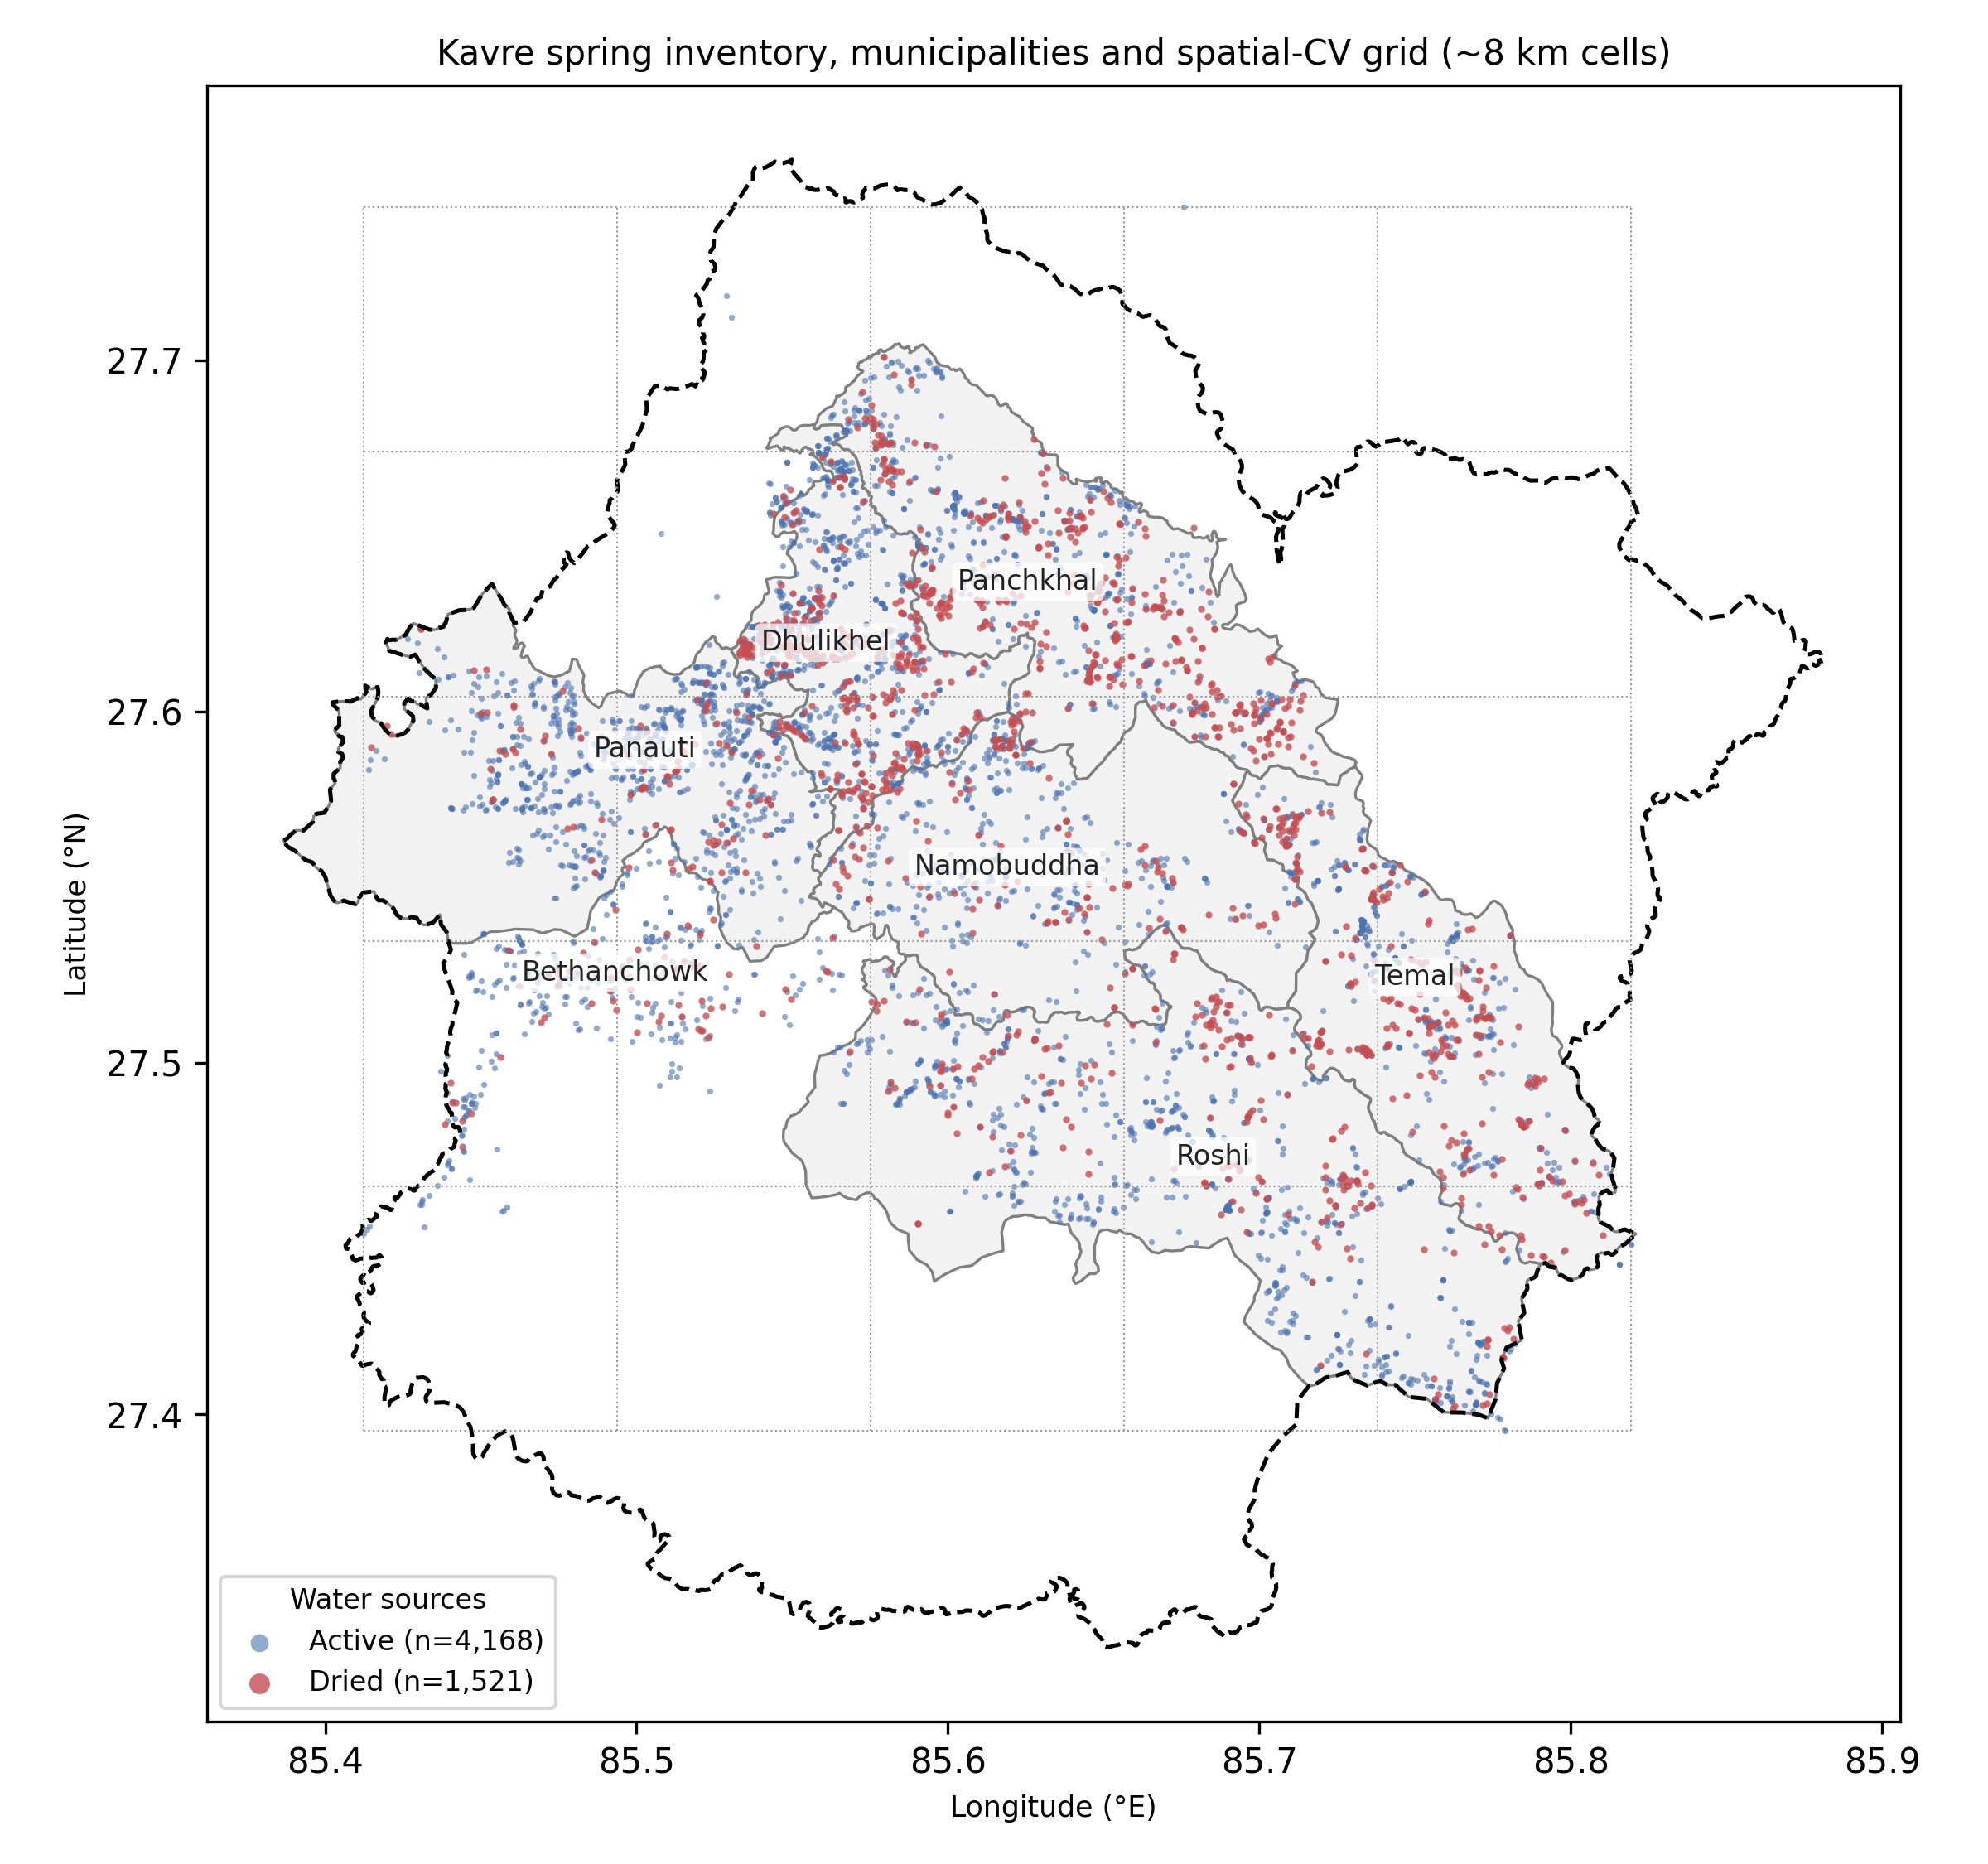
\includegraphics[width=0.72\linewidth]{study_area_map.png}
  \caption{Kavrepalanchok district (dashed), the seven surveyed municipalities (grey) and the 5,689 mapped water sources (blue: active; red: dried). Dotted lines: $5 \times 5$ grid ($\sim$\SI{8}{\kilo\metre}) used for spatial block cross-validation. Boundaries \copyright\ OpenStreetMap contributors (ODbL).}
  \label{fig:map}
\end{figure}

\subsection{Spring inventory and skip-logic audit}
The inventory \citep[CC BY 4.0;][]{icimod2025kavredata} covers 5,689 water sources (5,168 springs, 521 ponds) in 75 wards of seven municipalities, mapped between October 2023 and June 2024 \citep{thapa2025citizen}. A ward contains on average 76 sources, and 1,521 sources (26.7\%) are recorded as dried. For dried sources the survey also records the year of drying (Bikram Sambat calendar, BS) and a reason. The questionnaire has seven sections for active and four for dried sources, so 46 of 93 processed fields are outcome-dependent (Table~S2; Text~S1). These include every active-only question, among them \emph{``Any impact due to 2015 earthquake?''}, which is answered for 7 of 1,521 dried sources. No such field is used to build any unit, rule item or predictor. Dried-only fields are analysed only among dried sources.

\paragraph{What ``dried'' means.} The outcome is the questionnaire's \emph{source condition} (active or dried), as recorded by the resource person at the visit. The published data contain no operational criterion (e.g.\ zero flow on the visit day vs.\ no flow in the past year), no discharge measurement, no visit date and no enumerator identifier. The survey ran from October 2023 to June 2024, across the post-monsoon and dry seasons \citep{thapa2025citizen}, so a seasonal spring visited late in the dry season may have been recorded as dried. Two subgroups are therefore treated as sensitivity cases: the 521 ponds, of which 49\% are recorded as dried, against 24\% of springs, and the 930 sources flagged as seasonal, of which 63\% are recorded as dried. Every ward-level result was repeated for springs only, perennial sources only and perennial springs only (4,477 sources; Sect.~\ref{sec:res-sens}). We could not validate the label against discharge. The analysis therefore concerns \emph{recorded} drying throughout.

\subsection{GIS layers and Earth Engine enrichment}
\paragraph{Base layers.} Covariates come from independent layers (Table~\ref{tab:covariates}; Text~S2):
\begin{itemize}
  \item terrain from SRTM \citep{farr2007shuttle};
  \item catchment hydrology from MERIT Hydro \citep{yamazaki2019merit}: upstream area, height above nearest drainage (HAND), topographic wetness index \citep{beven1979physically}, topographic position (TPI) and ruggedness;
  \item climate from CHIRPS \citep{funk2015climate};
  \item water balance and decadal precipitation change from TerraClimate \citep{abatzoglou2018terraclimate};
  \item NDVI and NDWI from Sentinel-2 \citep{drusch2012sentinel};
  \item roads from OpenStreetMap \citep{osm2024}.
\end{itemize}

\paragraph{Enrichment.} From Google Earth Engine we added 28 label-free covariates:
\begin{itemize}
  \item ESA WorldCover land-cover fractions within \SI{250}{\metre} \citep{zanaga2022worldcover};
  \item Hansen tree cover and forest loss before and after 2015 \citep{hansen2013high};
  \item SoilGrids texture, organic carbon and bulk density \citep{poggio2021soilgrids};
  \item MODIS dry-season NDVI and evapotranspiration trends for 2001--2023 \citep{didan2021mod13q1, running2021mod16};
  \item the CHIRPS precipitation trend since 1981 and the 2015--2016 anomaly;
  \item GHSL built-up fraction and its change since 2000 \citep{pesaresi2023ghsl};
  \item WorldPop population \citep{worldpop2018} and VIIRS night lights \citep{elvidge2021annual};
  \item ALOS slope position, heat load (CHILI), multi-scale TPI and topographic diversity \citep{theobald2015ecologically}.
\end{itemize}
WorldCover agrees with the survey's own land-use record (\auc{} 0.75 for cropland, 0.76 for tree cover), which supports the survey field.

\paragraph{Covariate sets.} The \emph{landscape set} (46 covariates) contains only continuous, static GIS covariates. It excludes survey-recorded fields, so that landscape units are independent of the survey teams, and change variables, which may partly reflect drying. The \emph{environmental set} (65 covariates) adds survey structure and change variables and is used for partitioning and drivers. Prediction uses \texttt{env\_hydro} (39 covariates, the base layers) and the enriched \texttt{env\_rich} (67).

\paragraph{DEM routing and earthquake exposure.} An independent drainage network was derived from the Copernicus GLO-30 DEM \citep{esa2021copernicusdem} with D8 routing \citep{ocallaghan1984extraction}. Streams were defined at contributing areas of 0.5, 2 and \SI{10}{\kilo\metre\squared}; we computed Strahler order \citep{strahler1957quantitative} and link catchments and traced every source to its stream (Fig.~\ref{fig:hydro}). Sources occupy 619, 176 and 52 link catchments. Peak ground acceleration (PGA) of the 25 April and 12 May 2015 events was interpolated from USGS ShakeMap grids \citep{wald1999trinet, worden2012probabilistic, usgs2015shakemap}, and aftershock counts within \SI{20}{\kilo\metre} came from 283 ComCat events. Mainshock PGA (42--71\%$g$) increases eastward (Spearman $\rho = 0.87$ with longitude).

\begin{table}[t]
  \centering
  \caption{Covariate groups and their use. Definitions in Text~S2.}
  \label{tab:covariates}
  \small
  \begin{tabularx}{\linewidth}{lXll}
    \toprule
    Group & Covariates & Source & Use \\
    \midrule
    Terrain, morphometry & elevation, slope, aspect, TPI, ruggedness; slope position, CHILI, multi-scale TPI, topographic diversity & SRTM, ALOS & L, E, P \\
    Catchment hydrology & log upstream area, HAND, hydro-conditioned elevation, TWI & MERIT Hydro & L, E, P \\
    Climate, water balance & precipitation; AET, deficit, soil moisture, PDSI; precipitation change, trend and 2015 anomaly & CHIRPS, TerraClimate & L, E, P \\
    Vegetation, land cover & NDVI, NDWI; WorldCover fractions; tree cover 2000 & Sentinel-2, ESA, Hansen & L, E, P \\
    Soils & clay, sand, organic carbon, bulk density & SoilGrids & L, E, P \\
    Human footprint & roads; built-up fraction; population; night lights & OSM, GHSL, WorldPop, VIIRS & L, E, P \\
    Change & NDVI and ET trends, NDVI change 2015, forest loss 2015--23, built-up change & MODIS, Hansen, GHSL & E, P \\
    Survey (structural) & source type, land use, ownership, road upslope, source density & survey & E, P \\
    \midrule
    DEM routing & link catchments, flow length, Strahler order & Copernicus GLO-30 & analysis \\
    Seismic & PGA, PGV (25 April, 12 May), aftershock count and distance & USGS & analysis \\
    \bottomrule
  \end{tabularx}
  \\[2pt]\footnotesize L: landscape set (unsupervised analyses); E: environmental set (partitioning, drivers); P: prediction.
\end{table}

% =============================================================================
\section{Methods}\label{sec:methods}

Our design compares the homogeneity of drying within units defined in different ways, always against units of the same size placed at random, and tests every frequent pattern within wards. Table~\ref{tab:predictions} lists what a hydrological and a survey-process explanation predict for each test. No single test identifies survey process. The tests are diagnostic only jointly, and real ward-level physical differences can mimic several of them. Details are given in Texts~S3--S7.

\subsection{Unsupervised structure of the landscape}\label{sec:m-units}
\paragraph{Landscape types.} The landscape covariates were standardised and reduced by principal component analysis (PCA) to the 19 components explaining 90\% of variance. Gaussian mixtures \citep{fraley2002model} with $K = 2$--12 were compared by BIC \citep{schwarz1978estimating} and by bootstrap stability \citep{hennig2007cluster}, measured as the mean adjusted Rand index \citep[ARI;][]{hubert1985comparing} over 30 refits on 80\% subsamples. The selection rule was fixed before drying was examined: the lowest-BIC solution with mean ARI $\geq 0.75$ and no type below 2\% of sources. Density-based structure was examined with HDBSCAN \citep{campello2013density}, the geometry of landscape space with t-SNE \citep{vandermaaten2008visualizing}, and atypical settings with an isolation forest \citep{liu2008isolation}.

\paragraph{Label-free regionalisation.} Contiguous landscape regions were obtained by Ward clustering of the PCA scores constrained to a 10-nearest-neighbour graph, with 75 regions (the number of wards) and 176 regions (the number of \SI{2}{\kilo\metre\squared} DEM catchments). Louvain communities \citep{blondel2008fast} were detected on a 7-nearest-neighbour graph weighted by landscape similarity. For every partition (wards, municipalities, DEM catchments, landscape regions, communities) we computed two quantities:
\begin{itemize}
  \item \textbf{Landscape homogeneity:} the share of PCA variance explained by unit means.
  \item \textbf{Drying homogeneity:} the intraclass correlation ICC(1), compared with two null partitions.
\end{itemize}
The first null partition is a set of randomly shifted square grids. For each target partition with $m$ occupied units, the cell size was found by root-finding so that a grid at a reference origin also has $m$ occupied cells. 200 grids were then drawn with uniformly random origin offsets. Matching is on the number of occupied units, not on their size distribution. Shifted grids have on average 1--5\% more occupied cells than the target (78 for the 75 wards; Table~S23). Grid cells are compact, whereas wards are irregular and vary in size (16--164 sources, interquartile range 54--96). The second null, used for wards, therefore consists of 200 sets of \emph{contiguous random regions}. Each set is grown from random seeds on the 10-nearest-neighbour graph of sources, with target sizes drawn from the observed ward size distribution and compact, deficit-aware growth until every source is assigned (Text~S7). It preserves the number, size spread and contiguity of wards but not their boundaries.

\paragraph{Ward funnel plot.} Observed dried sources per ward were compared with those expected from a landscape-only logistic model, using funnel limits \citep{spiegelhalter2005funnel} and an overdispersion factor $\phi$, which is $\approx 1$ if wards differ only by chance given landscape.

\subsection{Apriori pattern mining}\label{sec:m-apriori}
Each source is a transaction. Its items are tertiles of 24 interpretable covariates (presence/absence where values are mostly tied), the landscape type, and survey source type, land use and ownership. Frequent itemsets were mined with apriori \citep{agrawal1994fast, raschka2018mlxtend} (support $\geq 2\%$, up to three items) and turned into rules \emph{A}~$\rightarrow$~dried and \emph{A}~$\rightarrow$~active. Rules were retained in four steps:
\begin{enumerate}
  \item Each rule is tested with a one-sided Fisher exact test, with Benjamini--Hochberg false-discovery control \citep{benjamini1995controlling}.
  \item Only \emph{productive} rules \citep{webb2007discovering} are kept: every item must raise confidence by $\geq 0.03$ over each generalisation.
  \item Rules are ranked by weighted relative accuracy \citep[WRAcc;][]{lavrac2004subgroup}.
  \item Each retained rule receives a Mantel--Haenszel odds ratio stratified by the 75 wards with its Robins--Breslow--Greenland interval \citep{robins1986general}, and a one-sided test of OR $> 1$. A rule is \emph{ward-robust} if this test is significant after a second Benjamini--Hochberg correction over all retained rules for that consequent ($q < 0.05$). Rules with pooled lift $>1$ but a within-ward interval entirely below 1 are Simpson-type reversals.
\end{enumerate}
Multiplicity is controlled at two levels. Pooled tests are corrected over \emph{all} candidate rules for each consequent (every frequent itemset, about 66,000 hypotheses). Within-ward tests are corrected over the retained rules (3,321 for drying, 2,337 for activity). The within-ward tests are applied to rules that were selected on the same data, and the stratified association is correlated with the pooled one. The ward-robust share is therefore a descriptive robustness summary of the selected set, not an independent confirmation. Selection-independent evidence comes only from held-out spatial blocks. Rules were re-mined on four of five $\sim$\SI{8}{\kilo\metre} blocks, and we report how often lift $>1$ held on the withheld block. The survey's seasonal-flow flag, which may encode dry-season fieldwork, was analysed separately. Narrative rules among dried sources use period, landscape type, survey attributes and municipality as items and reported causes as consequents.

\subsection{Spatial statistics}
\paragraph{Autocorrelation and scale.} Moran's $I$ \citep{moran1950notes} and local Moran's $I$ \citep{anselin1995local} with FDR control were computed. Variation in drying was partitioned with adjusted McFadden pseudo-$R^2$ \citep{peresneto2006variation} among environment ($E$), 250 Moran eigenvector maps \citep[$S$;][]{borcard2002allscale, dray2006spatial} and ward ($W$).

\paragraph{Pairs, direction and flow paths.} Pair concordance (31,693 pairs within 100--\SI{400}{\metre}) was modelled on same ward, same catchment and log distance. Upslope vs.\ downslope neighbour dependence was compared with a permutation null. Flow-path covariates were related to drying with and without environmental adjustment.

\paragraph{Scan statistic.} The Bernoulli scan statistic \citep{kulldorff1997spatial} was applied with 999 replicates. Intervals come from spatial-block bootstrap resamples.

\subsection{Recalled causes and years}\label{sec:m-dried}
Among dried sources, we computed the ICC of each reported cause (earthquake, drought, infrastructure) and of dating to 2072~BS (April 2015--April 2016) within wards, against size-matched grids, and within landscape types. The Knox test \citep{knox1964detection} counted pairs of dried sources within 250--\SI{1000}{\metre} reporting the same year, separately for pairs within a ward and across a ward boundary. If shared years reflect physical events, both kinds of pair should cluster; if they reflect shared reporting, only same-ward pairs should. Cross-boundary pairs are fewer (196 vs.\ 2,046 at \SI{250}{\metre}), so the across-ward test has less power, and a non-significant result means only that no clustering was detected. Wards with $\geq 8$ dried sources were clustered into \emph{narrative regimes} by their cause and period profiles (Hellinger geometry, Ward linkage, $K$ by silhouette). Mantel and partial Mantel tests \citep{mantel1967detection} then asked whether narrative similarity follows geography or landscape.

\subsection{Drivers, earthquake exposure, prediction and graphs}
\paragraph{Drivers and exposure.} Standardised coefficients of the environmental set were estimated pooled and with ward fixed effects. Earthquake exposure was related to drying with and without environmental adjustment, and, among dried sources, to attribution and dating. Because shaking varies mainly between wards, we report the share of exposure variance within wards. The exposure model was refitted with ward fixed effects and, as a softer spatial adjustment, with 100 broad- and meso-scale Moran eigenvector maps. Intervals come from a 200-replicate spatial-block bootstrap.

\paragraph{Prediction.} Logistic regression, random forest, XGBoost \citep{chen2016xgboost}, CatBoost \citep{prokhorenkova2018catboost}, a multilayer perceptron (MLP), kNN label interpolation, a residual GATv2 with terrain edge attributes and a CatBoost--GAT hybrid (HydroBoost-GAT) were evaluated in three designs:
\begin{itemize}
  \item spatial block cross-validation on $\sim$\SI{8}{\kilo\metre} blocks (5 folds $\times$ 5 seeds);
  \item the same with buffers of 500, 1,000 and \SI{2000}{\metre} that remove training sources near any test source \citep{roberts2017cross, valavi2019blockcv, ploton2020spatial};
  \item leave-one-municipality-out (LOMO), a contiguous-region holdout.
\end{itemize}
Blocks are assigned to folds, so test and training sources can be adjacent across block edges. Without a buffer, the median distance from a test source to its nearest training source is \SI{1.9}{\kilo\metre}, but 10\% of test sources lie within \SI{500}{\metre} and 25\% within \SI{1}{\kilo\metre} (Table~S53). The scores therefore describe prediction into partly surveyed $\sim$\SI{8}{\kilo\metre} blocks. They are an optimistic proxy for deployment to an unsurveyed area, which wider buffers and LOMO approach more closely \citep{wadoux2021spatial, meyer2022machine}. Differences were tested with the corrected resampled $t$-test \citep{nadeau2003inference, bouckaert2004evaluating} and Holm adjustment.

\paragraph{Graph topologies.} GraphSAGE and the residual GATv2 were trained on five graphs and compared with an identically trained MLP:
\begin{itemize}
  \item geographic nearest neighbours;
  \item nearest neighbours within the same DEM catchment;
  \item a ridge-aware graph;
  \item nearest neighbours within the same ward;
  \item random links.
\end{itemize}

\begin{table}[t]
  \centering
  \caption{Predictions of hydrological and survey-process explanations, and the outcome of each test (Sect.~\ref{sec:results}). Real ward-level physical or management differences can produce several of the survey-process outcomes (rows marked $^\ast$). No row identifies survey process on its own.}
  \label{tab:predictions}
  \small
  \begin{tabularx}{\linewidth}{>{\raggedright\arraybackslash}p{3.7cm}XXX}
    \toprule
    Test & Hydrological control & Survey-process effect & Result \\
    \midrule
    Drying ICC, DEM catchments vs.\ grids & above & no difference & no difference \\
    Drying ICC, landscape regions vs.\ grids & above & no difference & above (all sources); not with seasonal sources excluded \\
    Drying ICC, wards vs.\ grids and random regions$^\ast$ & above only if wards are landscape units & above & above both nulls; wards not landscape units \\
    Ward funnel vs.\ landscape model$^\ast$ & $\phi \approx 1$ & $\phi \gg 1$ & $\phi = 5.3$--6.3 \\
    Pair concordance$^\ast$ & same catchment & same ward & same ward only \\
    Upslope vs.\ downslope neighbours & upslope stronger & symmetric & no asymmetry detected \\
    Apriori rules & hold within wards & reverse or vanish within wards & 79\% ward-robust; 15 reverse \\
    Knox same-year clustering & within and across wards & within wards only & detected within wards only (across: low power) \\
    Recalled cause/year ICC & types $\approx$ wards & wards $\gg$ types & wards $\gg$ types \\
    Narrative similarity of wards & follows landscape & no relation to landscape or geography & no association detected \\
    Spatial fraction of variation$^\ast$ & shared with environment & shared with wards & shared with wards \\
    \bottomrule
  \end{tabularx}
\end{table}

% =============================================================================
\section{Results}\label{sec:results}

\subsection{Leakage and leak-free predictability}
An indicator of whether the earthquake question was answered predicts drying with \auc{} 0.958 on its own (Table~S3). Adding the two earthquake encodings lifts every model to \auc{} 0.982--0.987 (Table~S6). With leak-free covariates (Table~\ref{tab:benchmark}):
\begin{itemize}
  \item With the base layers, \auc{} under spatial cross-validation is 0.665--0.685, and 0.614--0.639 for an unseen municipality.
  \item With the Earth Engine enrichment, \auc{} rises slightly, to 0.664--0.692 (random forest 0.692 $\pm$ 0.060, and 0.691 with a \SI{500}{\metre} buffer).
  \item No model differs significantly from the best tabular model except kNN label interpolation (0.598).
  \item Performance declines gradually as test sources are moved further from training data. For the random forest with base layers, \auc{} is 0.683 without a buffer, 0.681 at \SI{500}{\metre}, 0.671 at \SI{1}{\kilo\metre}, 0.651 at \SI{2}{\kilo\metre} and 0.635 for LOMO. Logistic regression and CatBoost follow the same pattern (0.650 and 0.642 at \SI{2}{\kilo\metre}; Table~S6).
\end{itemize}
Earthquake exposure adds nothing. The seasonal-flow flag raises \auc{} to 0.72--0.75 but plausibly reflects dry-season fieldwork (Sect.~\ref{sec:res-apriori}).

\begin{table}[t]
  \centering
  \caption{Leak-free predictability: \auc{} mean $\pm$ SD over seed--fold pairs (spatial CV $5 \times 5$; LOMO 3 seeds $\times$ 7 municipalities). Base: \texttt{env\_hydro} (39 covariates); enriched: \texttt{env\_rich} (67). Test prevalence 0.27. --: not run. Apart from kNN interpolation, no model differs significantly from the best tabular model (Tables~S4--S6).}
  \label{tab:benchmark}
  \small
  \begin{tabular}{lcccc}
    \toprule
    Model & Base, no buffer & Base, \SI{500}{\metre} & Base, LOMO & Enriched, no buffer \\
    \midrule
    Logistic regression & 0.669 $\pm$ 0.052 & 0.668 $\pm$ 0.052 & 0.630 $\pm$ 0.035 & 0.664 $\pm$ 0.064 \\
    Random forest       & 0.683 $\pm$ 0.061 & 0.681 $\pm$ 0.056 & 0.635 $\pm$ 0.046 & 0.692 $\pm$ 0.060 \\
    XGBoost             & 0.672 $\pm$ 0.057 & 0.665 $\pm$ 0.054 & -- & 0.676 $\pm$ 0.056 \\
    CatBoost            & 0.678 $\pm$ 0.057 & 0.670 $\pm$ 0.056 & 0.639 $\pm$ 0.043 & 0.684 $\pm$ 0.052 \\
    kNN label interpolation & 0.598 $\pm$ 0.043 & 0.595 $\pm$ 0.051 & 0.513 $\pm$ 0.071 & -- \\
    MLP                 & 0.666 $\pm$ 0.058 & 0.668 $\pm$ 0.057 & 0.616 $\pm$ 0.046 & 0.680 $\pm$ 0.059 \\
    Residual GATv2      & 0.665 $\pm$ 0.058 & 0.662 $\pm$ 0.058 & 0.614 $\pm$ 0.048 & -- \\
    HydroBoost-GAT      & 0.685 $\pm$ 0.057 & 0.678 $\pm$ 0.057 & 0.633 $\pm$ 0.042 & -- \\
    \bottomrule
  \end{tabular}
\end{table}

\subsection{Landscape types structure drying}\label{sec:res-types}
The 46 landscape covariates reduce to 19 principal components (90\% of variance). The leading axes are a soil-carbon, forest-cover and elevation gradient (PC1, 24\%), a water-balance and built-up gradient (PC2, 15\%) and a slope-position gradient (PC3, 10\%: ALOS slope position, HAND, multi-scale TPI vs.\ TWI and upstream area). The selection rule picks eight types (mean bootstrap ARI 0.84; Table~S9). Although built without labels or survey fields, they differ threefold in drying (Table~\ref{tab:types}; Fig.~\ref{fig:types}; $\chi^2 = 230$, 7 df). Two types are notably dry:
\begin{itemize}
  \item \textbf{Peri-urban, built-up settings} (T1: 40\% dried). Infrastructure accounts for 56\% of their reported causes, against 16\% overall.
  \item \textbf{Steep, water-limited mid-slopes high above drainage} (T5: 37\%).
\end{itemize}
High, wet, organic-soil forest (T8) dries least (13\%).

Type remains informative within wards (likelihood-ratio $\chi^2 = 55.9$, 7 df, $p < 10^{-8}$), but it explains far less than ward does (adjusted pseudo-$R^2$ 0.034 vs.\ 0.106; Cram\'er's $V$ with drying 0.20 vs.\ 0.36; Table~S12). The types partition a continuum rather than discrete clusters. HDBSCAN finds only two density clusters, labels 44\% of sources as noise and agrees with the mixture types at chance level (ARI 0.04; Tables~S14--S15). Landscape anomalies (5\%, isolation forest) are more often dried (33.7\% vs.\ 26.4\%; OR 1.42, $p = 0.007$; Table~S16). Anomalies are concentrated in built-up (24\% of T1 sources flagged) and valley-corridor settings (43\% of T4) (Fig.~\ref{fig:embedding}).

\begin{table}[t]
  \centering
  \caption{Landscape types from 46 continuous GIS covariates (no labels, no survey fields), ordered by drying rate; 95\% Wilson intervals. Profiles in Table~S11.}
  \label{tab:types}
  \small
  \begin{tabular}{llrcc}
    \toprule
    Type & Setting & $n$ & Wards & Drying rate [95\% CI] \\
    \midrule
    T1 & Peri-urban: built-up, roads, night lights, low NDVI & 305 & 14 & 0.400 [0.347, 0.456] \\
    T5 & Steep, water-limited mid-slopes high above drainage & 1,514 & 48 & 0.369 [0.345, 0.393] \\
    T2 & Low cultivated flats, dense soils, high water deficit & 471 & 23 & 0.295 [0.256, 0.338] \\
    T3 & Dry low-precipitation slopes & 759 & 33 & 0.295 [0.264, 0.329] \\
    T4 & Valley-bottom river corridors (bare, water) & 203 & 38 & 0.261 [0.205, 0.326] \\
    T7 & Forested steep upper slopes, wetting trend & 1,037 & 55 & 0.198 [0.175, 0.223] \\
    T6 & Moist cultivated mid-elevation slopes & 741 & 24 & 0.185 [0.159, 0.214] \\
    T8 & High, wet, organic-soil forest & 659 & 12 & 0.126 [0.103, 0.153] \\
    \bottomrule
  \end{tabular}
\end{table}

\begin{figure}[t]
  \centering
  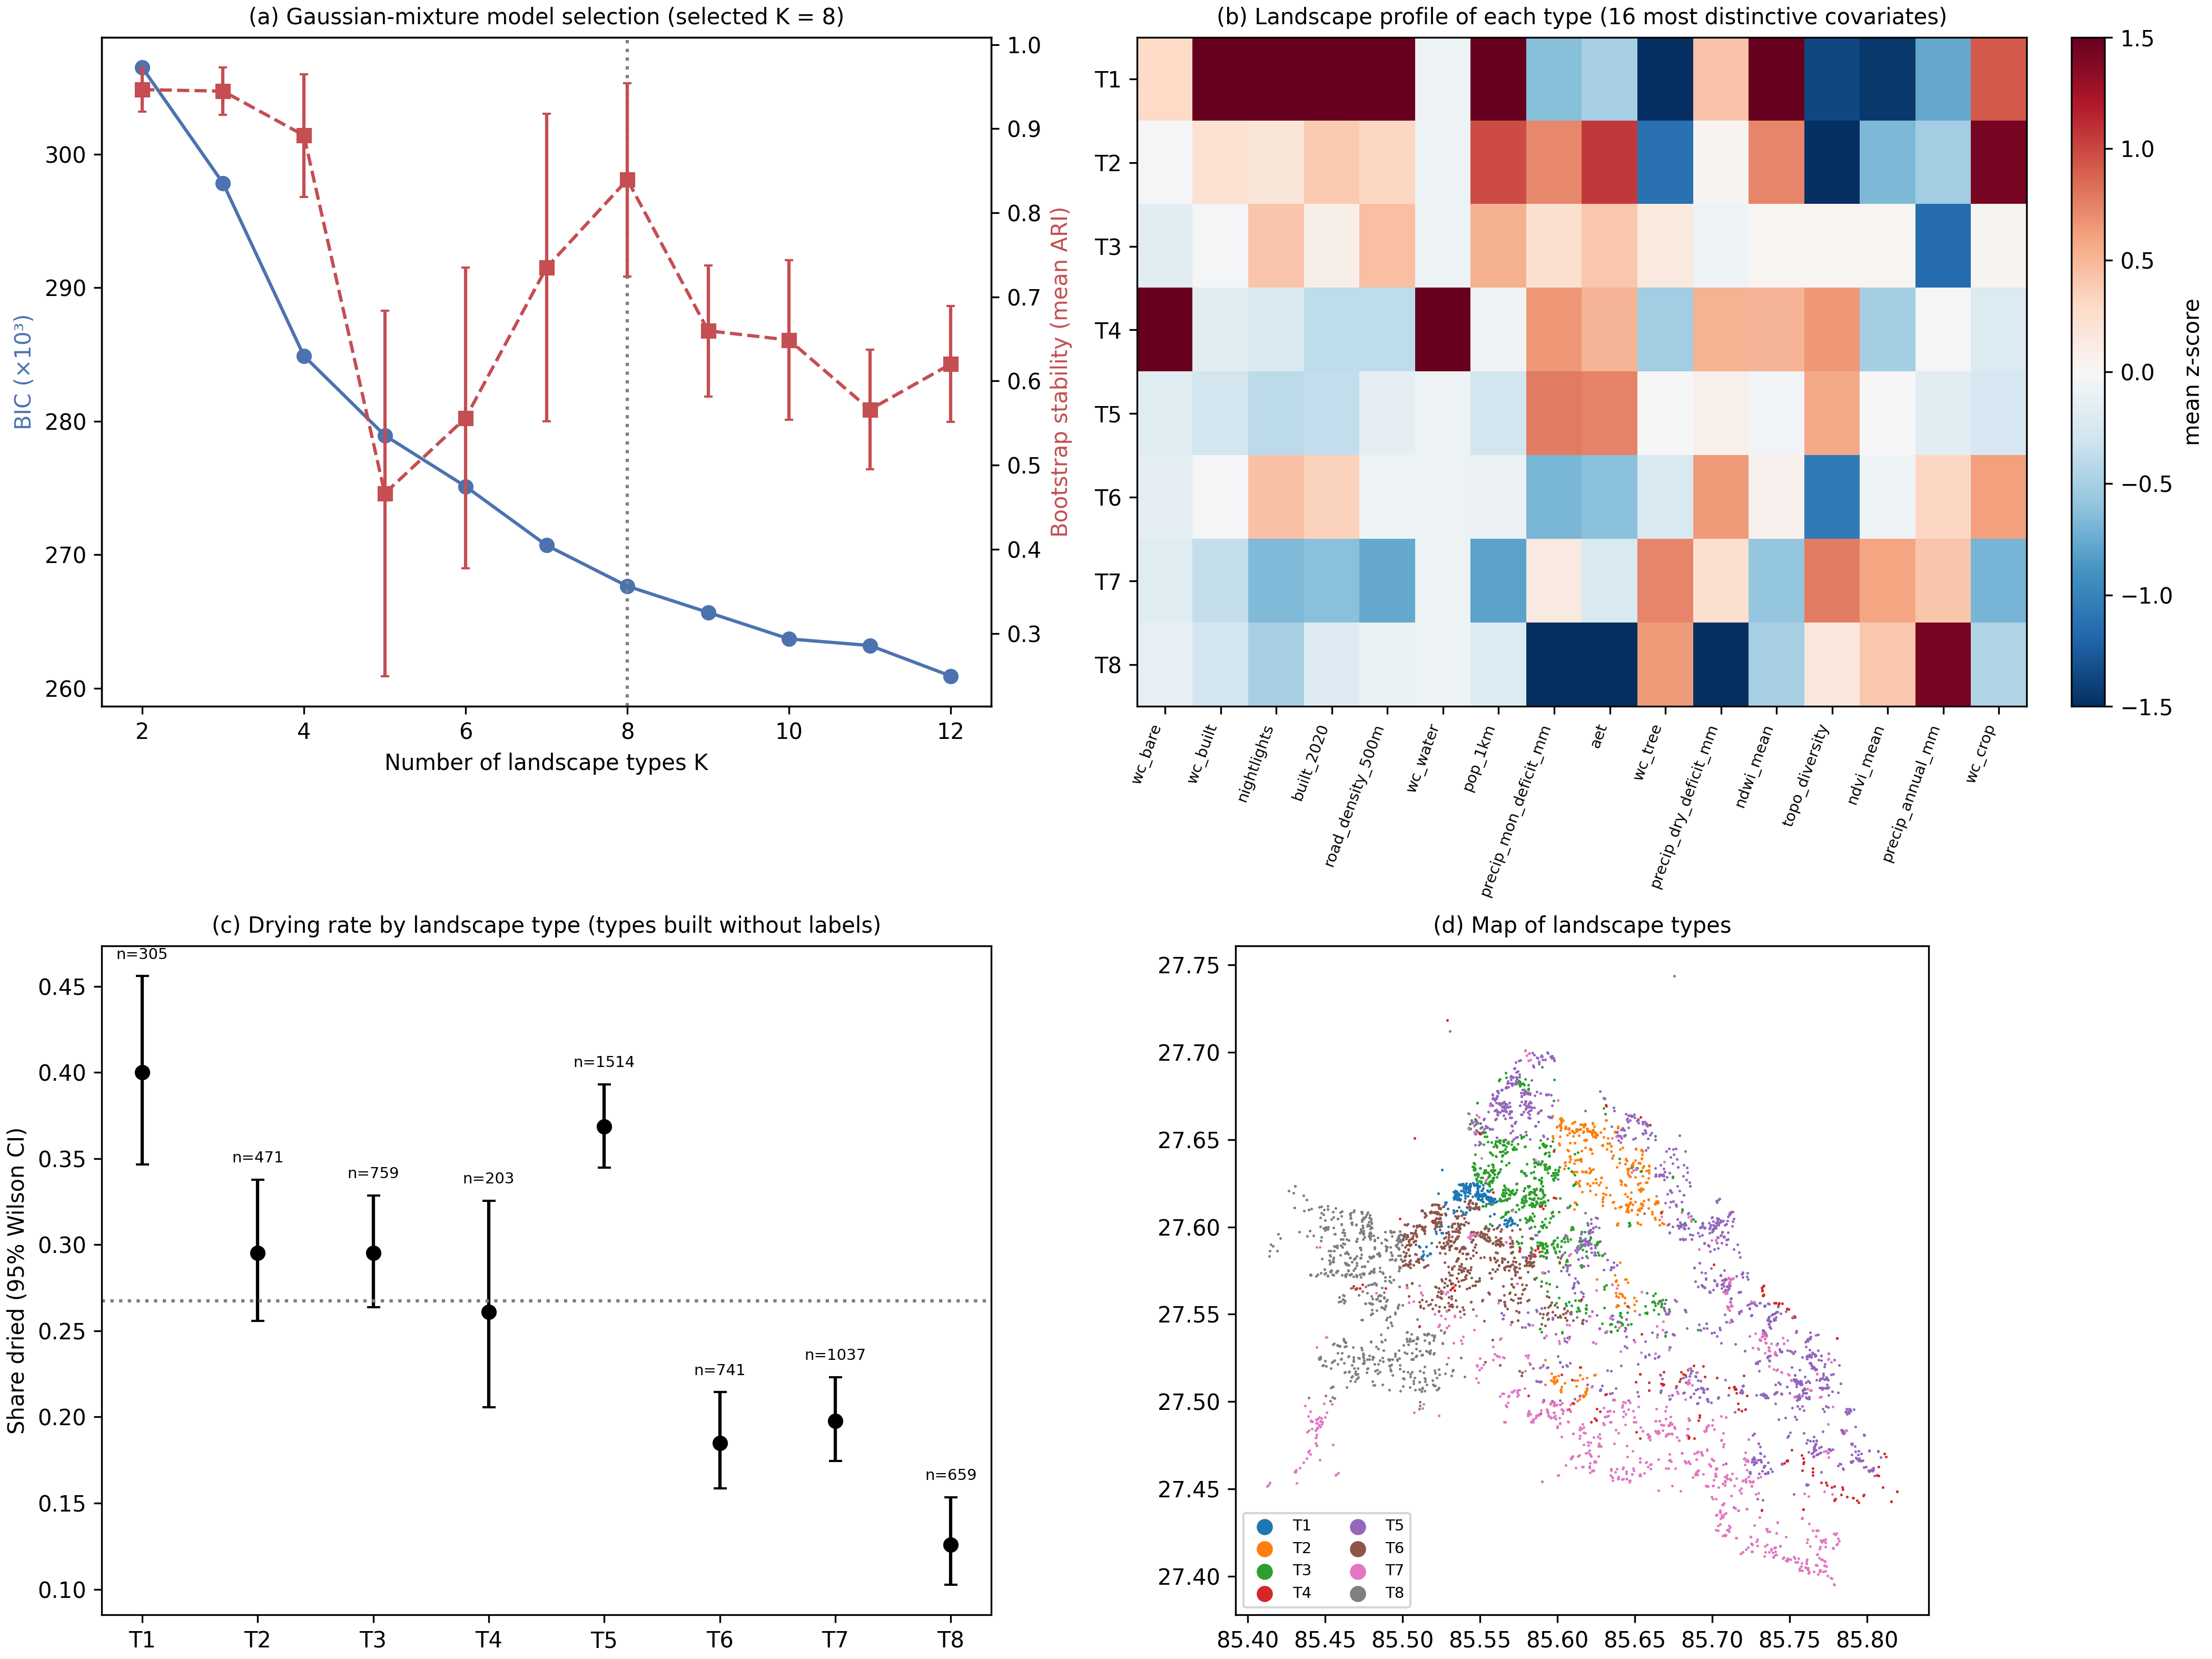
\includegraphics[width=\linewidth]{un_typology.png}
  \caption{Landscape typology. (a) BIC and bootstrap stability (mean ARI $\pm$ SD) of Gaussian mixtures; dotted line: selected solution. (b) Mean standardised covariates of each type (16 most distinctive). (c) Drying rate by type (95\% Wilson intervals). (d) Map of types.}
  \label{fig:types}
\end{figure}

\begin{figure}[t]
  \centering
  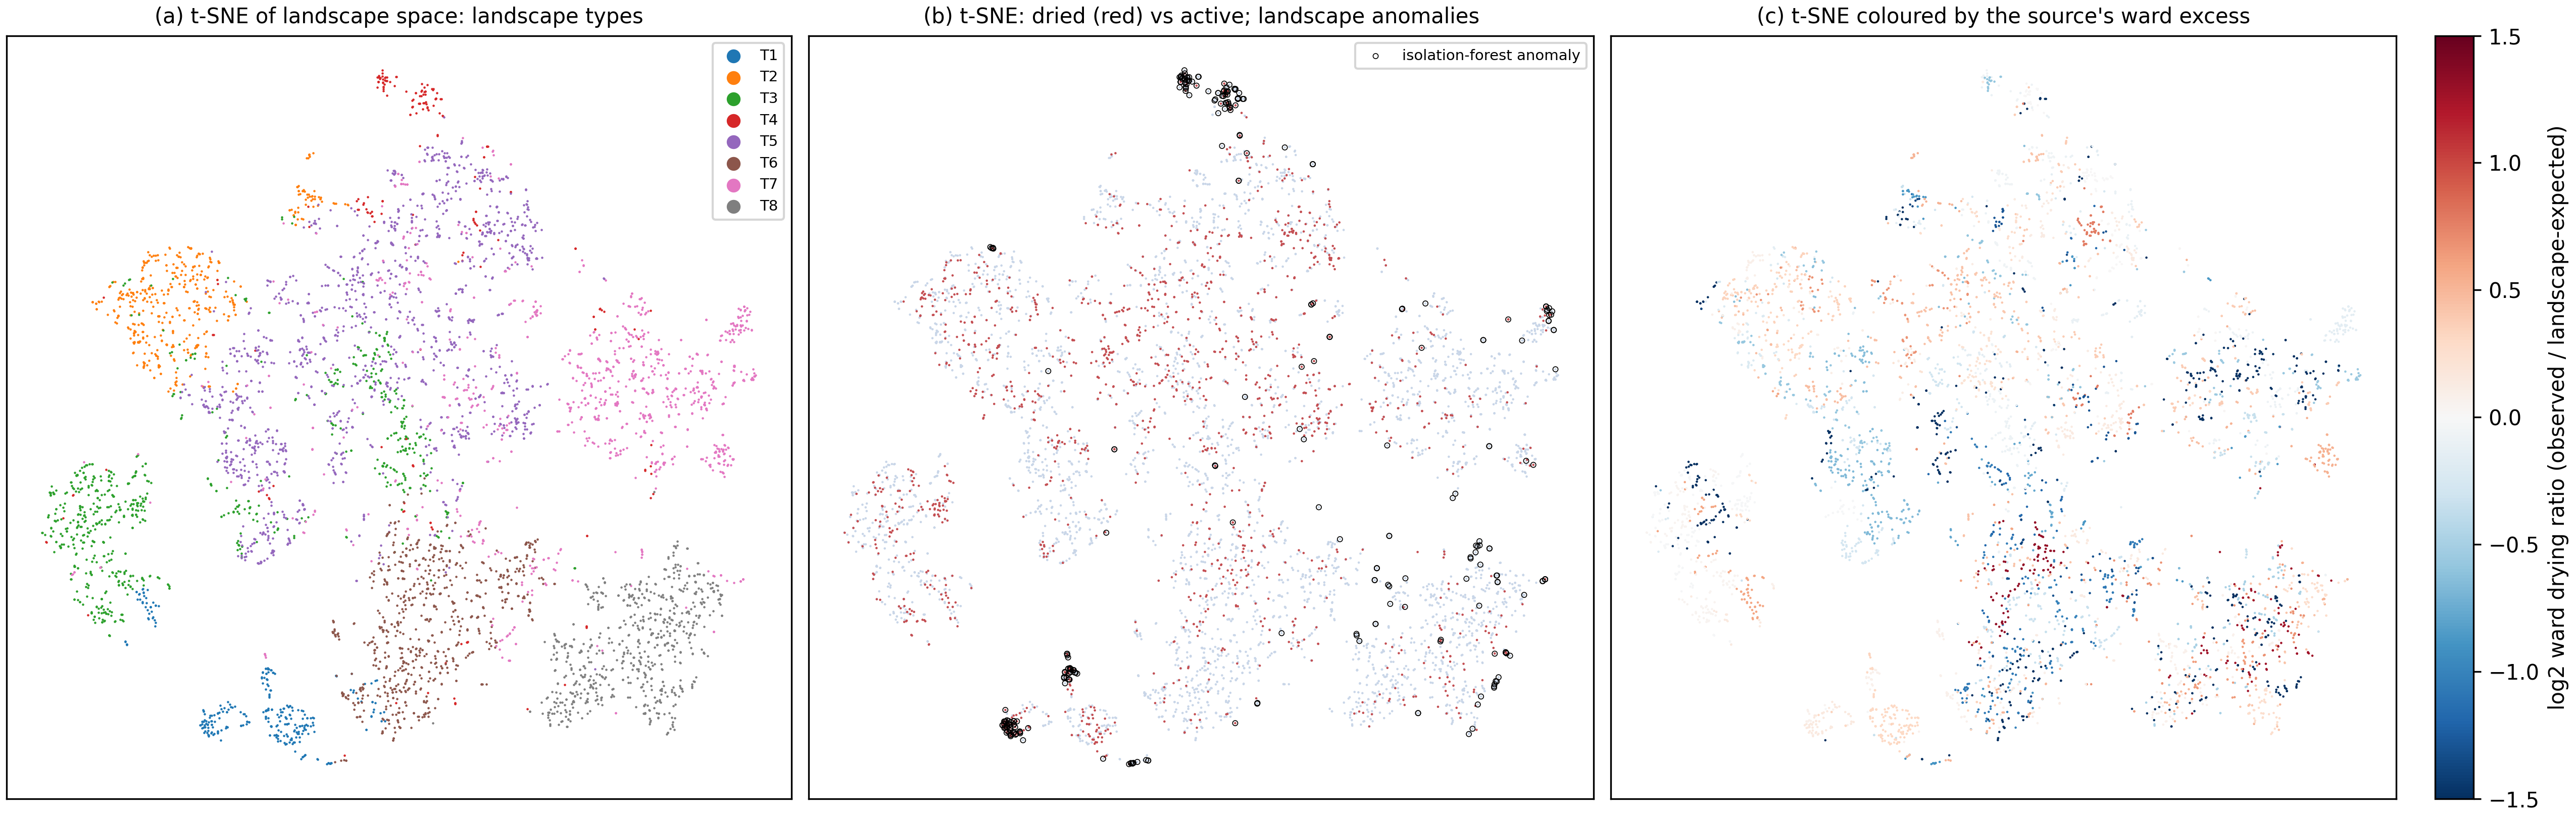
\includegraphics[width=\linewidth]{un_embedding.png}
  \caption{t-SNE embedding of landscape space coloured by (a) landscape type, (b) status (red: dried) with isolation-forest anomalies circled, and (c) the drying excess of each source's ward over the landscape-only expectation.}
  \label{fig:embedding}
\end{figure}

\subsection{Frequent patterns of drying}\label{sec:res-apriori}
Apriori found 66,563 frequent itemsets. After FDR control and productivity pruning, 3,321 of 15,744 significant rules for drying and 2,337 of 18,580 for activity remain (Table~S32). As a robustness summary of this selected set, 79\% and 81\% respectively remain significant within wards (Mantel--Haenszel, BH $q < 0.05$), and the median rule keeps lift $>1$ on every held-out spatial block (78\% and 86\% on at least four of five). Ward-robust rules concentrate at high lift. Rules with lift below about 1.5 are often not robust within wards (Fig.~\ref{fig:rules}a). The most robust risk patterns involve topographic position and water balance (Fig.~\ref{fig:rules}; Table~S34):
\begin{itemize}
  \item high TPI: confidence 0.36, within-ward OR 2.27 [1.97, 2.62], lift $> 1$ in 85\% of wards;
  \item high multi-scale TPI: OR 1.89;
  \item high HAND: OR 2.07;
  \item high climatic water deficit: OR 1.51;
  \item their conjunctions, e.g.\ HAND high \& deficit high: confidence 0.52, OR 2.68 [2.17, 3.30].
\end{itemize}
The protective counterparts are stronger. ``TPI low \& soil moisture high'' has confidence 0.93 for active sources, OR 4.03 [2.90, 5.61], and lift $> 1$ in 96\% of wards. ``Climatic water deficit low \& upstream area high'' has confidence 0.91 and OR 2.97.

Fifteen rules reverse within wards. ``Elevation low $\rightarrow$ dried'' has pooled lift 1.28 but a within-ward OR of 0.80 [0.67, 0.97]: low-elevation wards dry more, but within a ward, low-lying sources do not. Several rules combining high population with low precipitation trends behave similarly (Table~S34).

The survey's seasonal-flow flag, mined separately, is the strongest single item. 63.1\% of sources recorded as seasonal are recorded as dried, against 19.6\% of perennial sources (within-ward OR 6.9 [5.8, 8.4]; Table~S33), consistent with dry-season visits recording seasonal springs as dried.

\begin{figure}[t]
  \centering
  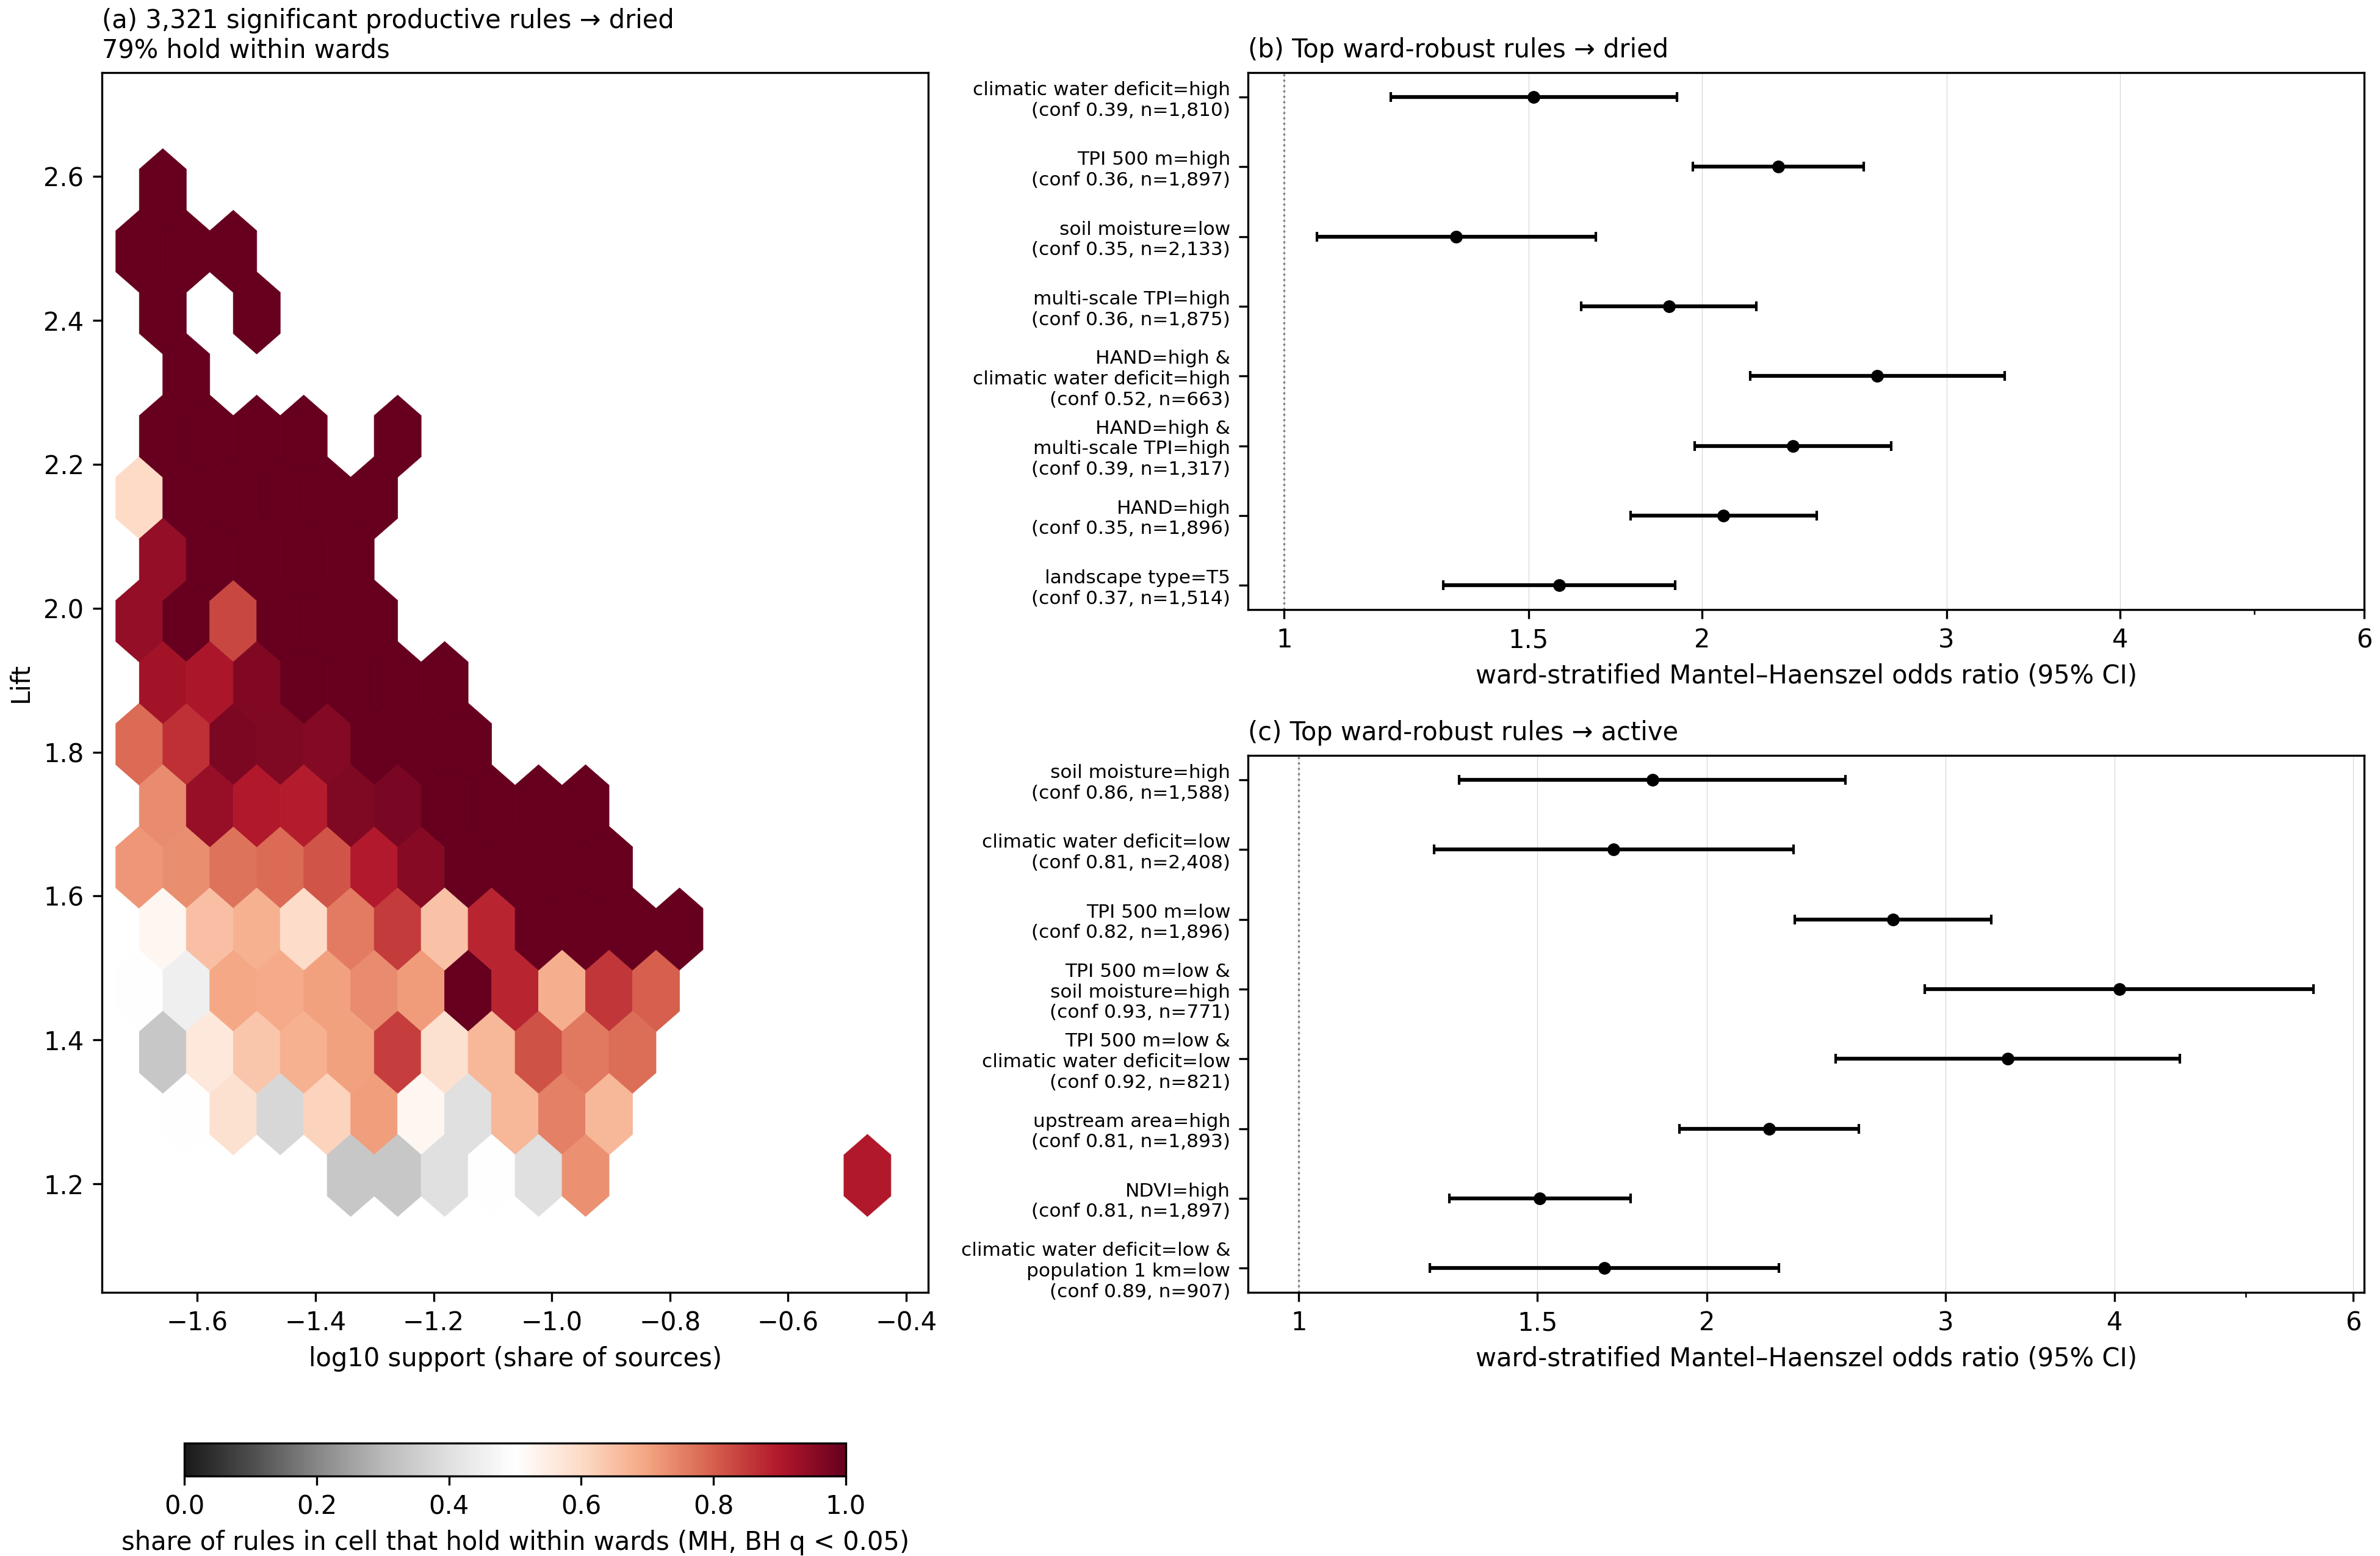
\includegraphics[width=\linewidth]{pm_rules.png}
  \caption{Apriori rules. (a) All 3,321 significant productive rules for drying, binned by support and lift. Colour shows the share of rules in each cell that remain significant within wards (Mantel--Haenszel, BH $q < 0.05$); cells with fewer than three rules are omitted. (b, c) The eight top ward-robust rules for drying and for activity, ranked by WRAcc, with ward-stratified Mantel--Haenszel odds ratios (95\% CI). Confidence and number of sources are given in brackets.}
  \label{fig:rules}
\end{figure}

\subsection{Spatial structure and scales}
Drying is autocorrelated: Moran's $I$ falls from 0.279 at $k = 3$ (mean distance \SI{162}{\metre}) to 0.179 at $k = 20$ (\SI{477}{\metre}). Local Moran's $I$ identifies 95 sources in FDR-significant dried clusters (Tables~S17--S18). The environment explains 0.112 and Moran eigenvector maps 0.087 of variation (adjusted pseudo-$R^2$). The spatial fraction not shared with environment (0.034) lies mostly at meso scales (MEMs 26--100; Tables~S19--S20). The scan statistic finds eight clusters of elevated and eight of reduced drying. The largest are regional (eastern Panchkhal and Temal high, western Panauti low) and span up to 16 wards (Fig.~\ref{fig:mining}f; Tables~S21--S22).

\subsection{Wards, not watersheds}\label{sec:res-wards}
\paragraph{Homogeneity.} DEM catchments are no more homogeneous in drying than random squares at any threshold (ICC 0.161, 0.122 and 0.088 against 0.169--0.200, 0.115--0.135 and 0.073--0.100; Fig.~\ref{fig:hydro}; Table~S23). Landscape units are (Table~S24):
\begin{itemize}
  \item 75 landscape regions: ICC 0.113;
  \item 176 landscape regions: 0.153;
  \item 94 Louvain communities: 0.132;
\end{itemize}
all above every matched grid ($p = 0.005$). The advantage of the 75 landscape regions is lost when seasonal sources are excluded (Sect.~
ef{sec:res-sens}). Wards differ from all landscape units. They are no more homogeneous in landscape than random squares (share of landscape variance 0.52 vs.\ 0.50, against 0.65 for landscape regions), and they agree with landscape regions no better than random squares do (ARI 0.37 vs.\ 0.41). Yet their drying ICC (0.132) exceeds every matched grid (0.093--0.106) and every set of contiguous random regions with the ward size distribution (0.081--0.111; both $p = 0.005$; Fig.~\ref{fig:robust}a). It equals that of the best landscape partition of similar size.

\paragraph{Funnel plot.} Against a landscape-only model, 26 of 75 wards lie outside 95\% limits (3.75 expected) and 13 outside 99.8\% limits (0.15 expected; six high, seven low). The overdispersion factor is $\phi = 5.5$, and observed/expected ratios range from 0.11 to 2.49 (Fig.~\ref{fig:wards}a; Tables~S30--S31).

\paragraph{Pairs, direction and flow.} Same-ward pairs share status more often at every distance (0--\SI{100}{\metre}: 0.75 vs.\ 0.62; 200--\SI{400}{\metre}: 0.65 vs.\ 0.55). Jointly, the same ward raises the odds of concordance 1.56-fold (1.01--1.82), whereas the same catchment does not (1.11; 0.97--1.27; Tables~S25--S26). No asymmetry between upslope and downslope neighbours was detected ($\beta_{\text{up}} - \beta_{\text{down}} = 0.06$, $p = 0.41$; Table~S27). No flow-path covariate is associated with drying after environmental adjustment (Table~S28).

\paragraph{Variation partitioning.} Ward alone explains almost as much as the 65 environmental covariates (0.106 vs.\ 0.112). Of the 0.087 explained by space, 0.077 is shared with wards, and the fraction unique to space is $-0.002$. Environment retains a unique 0.050 (Table~\ref{tab:partition}).

\begin{figure}[t]
  \centering
  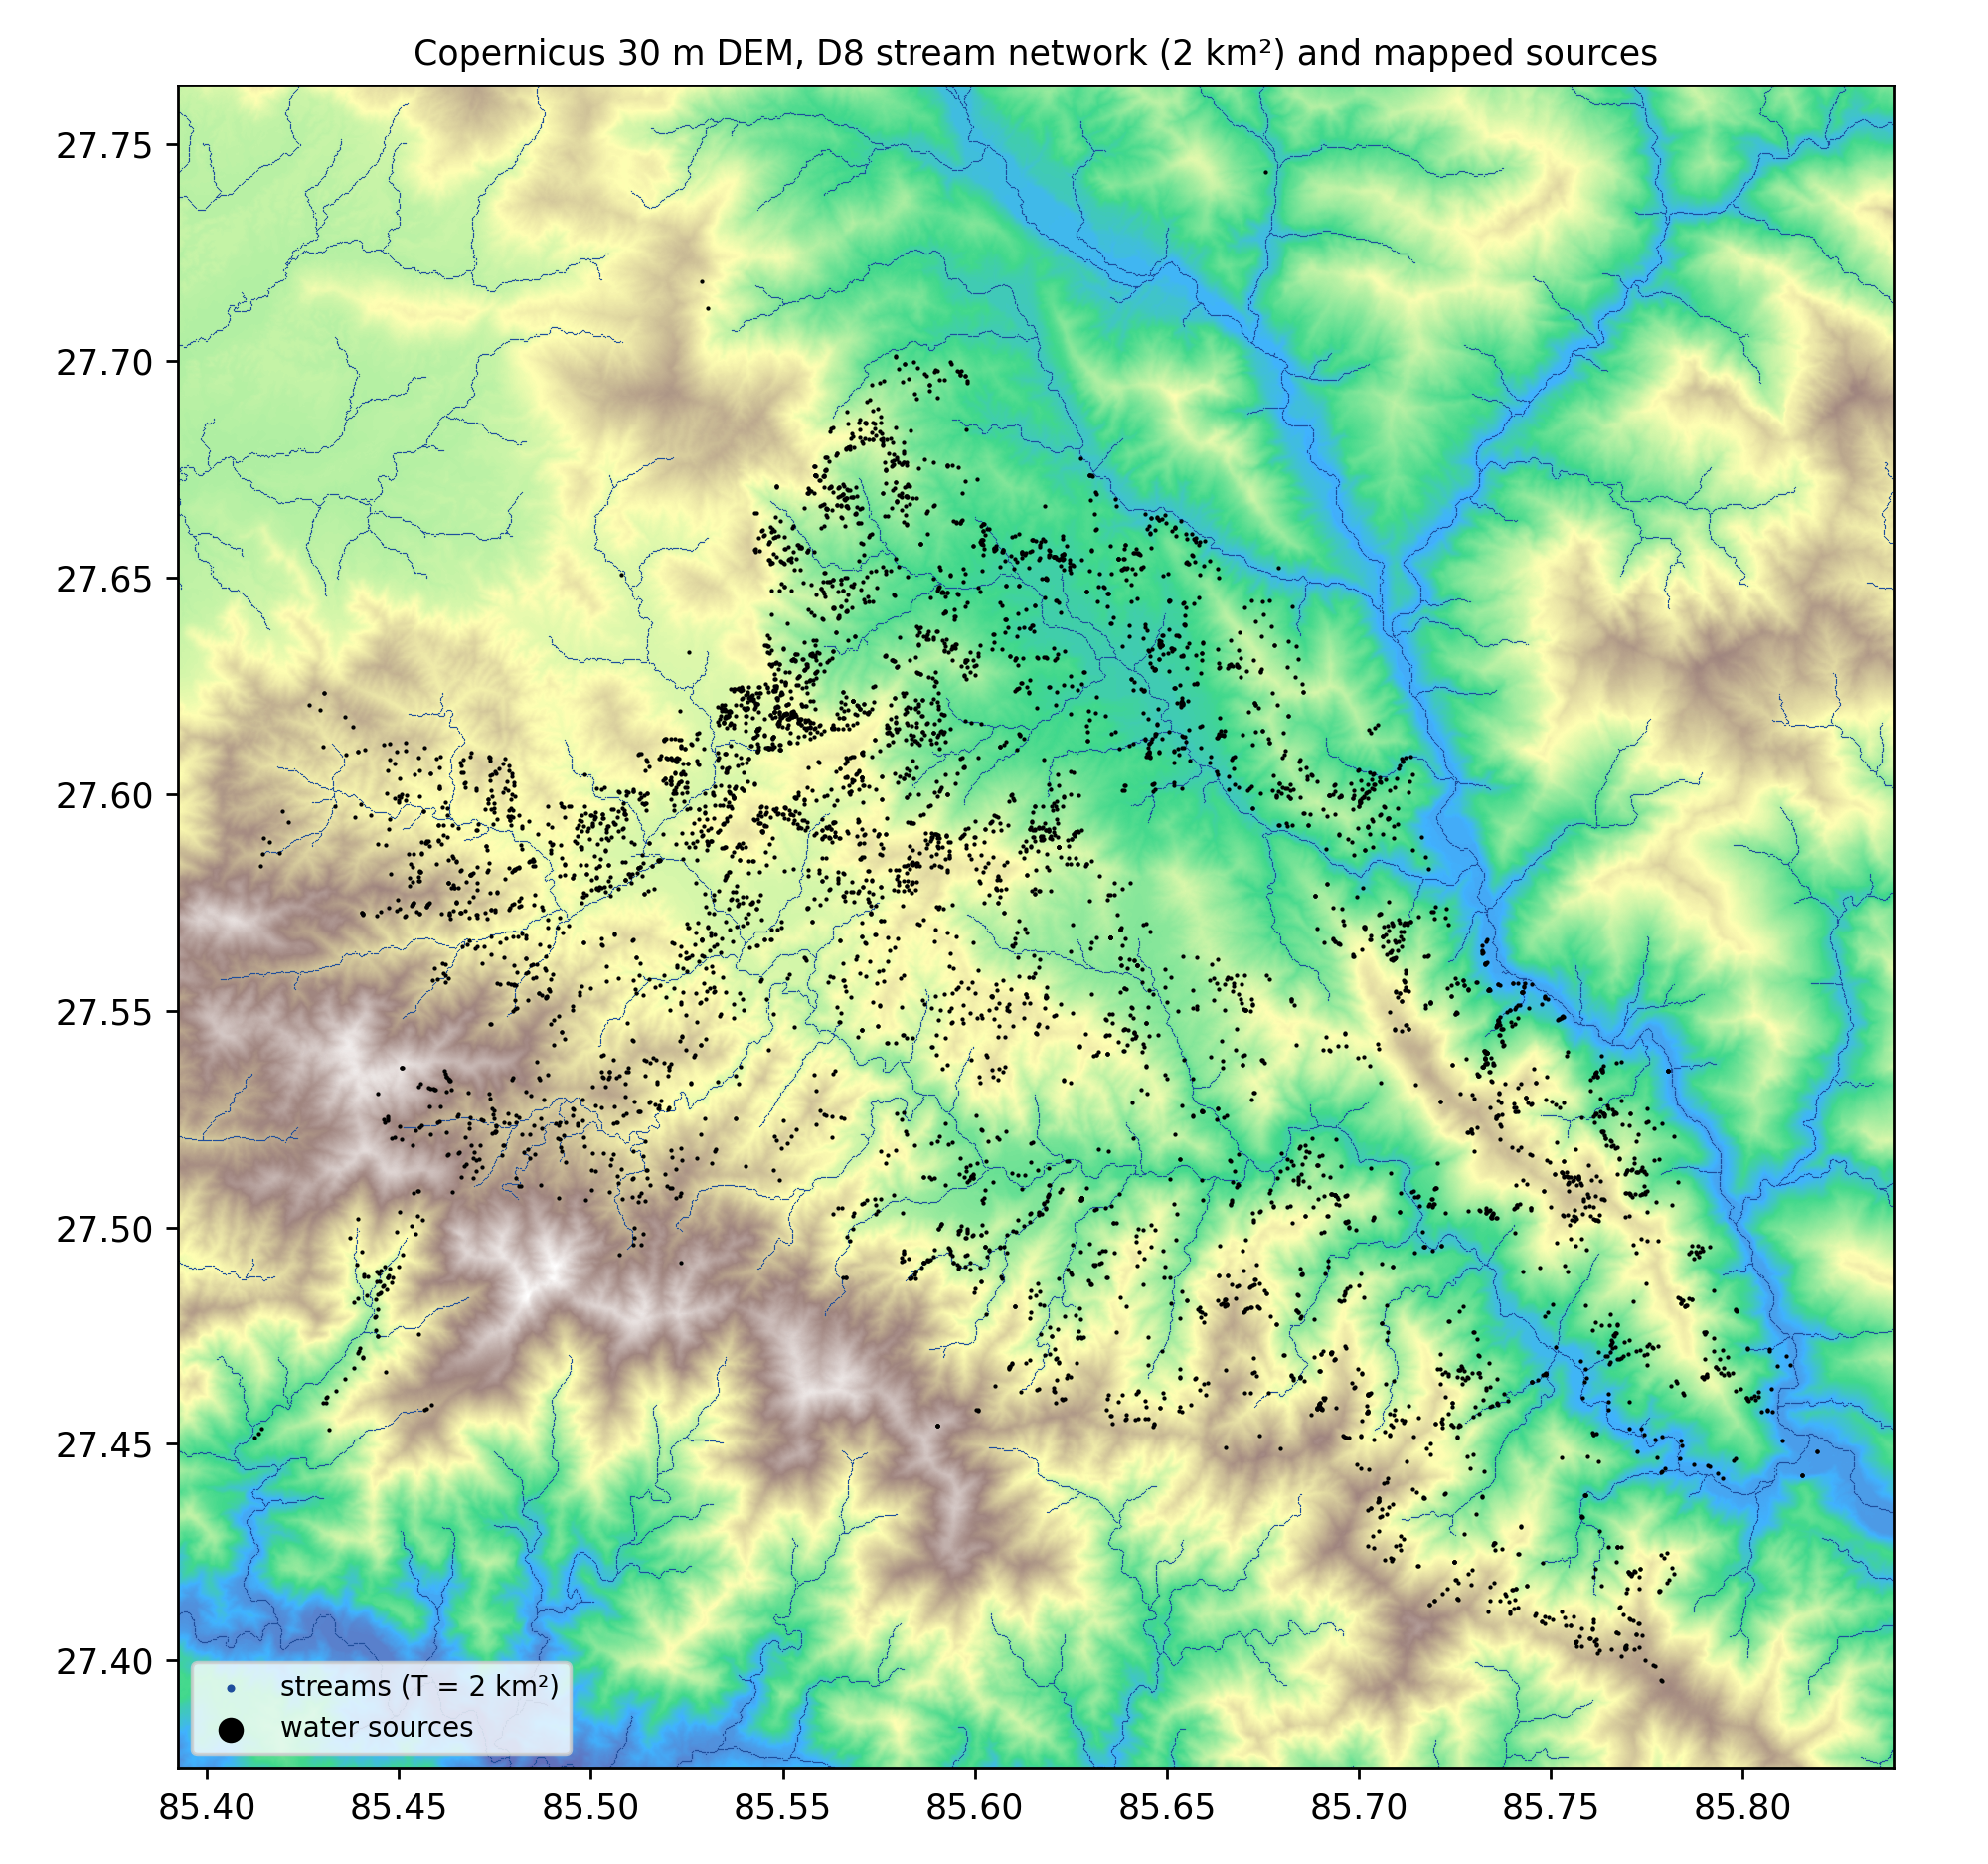
\includegraphics[width=0.34\linewidth]{hydro_gis_network.png}\hfill
  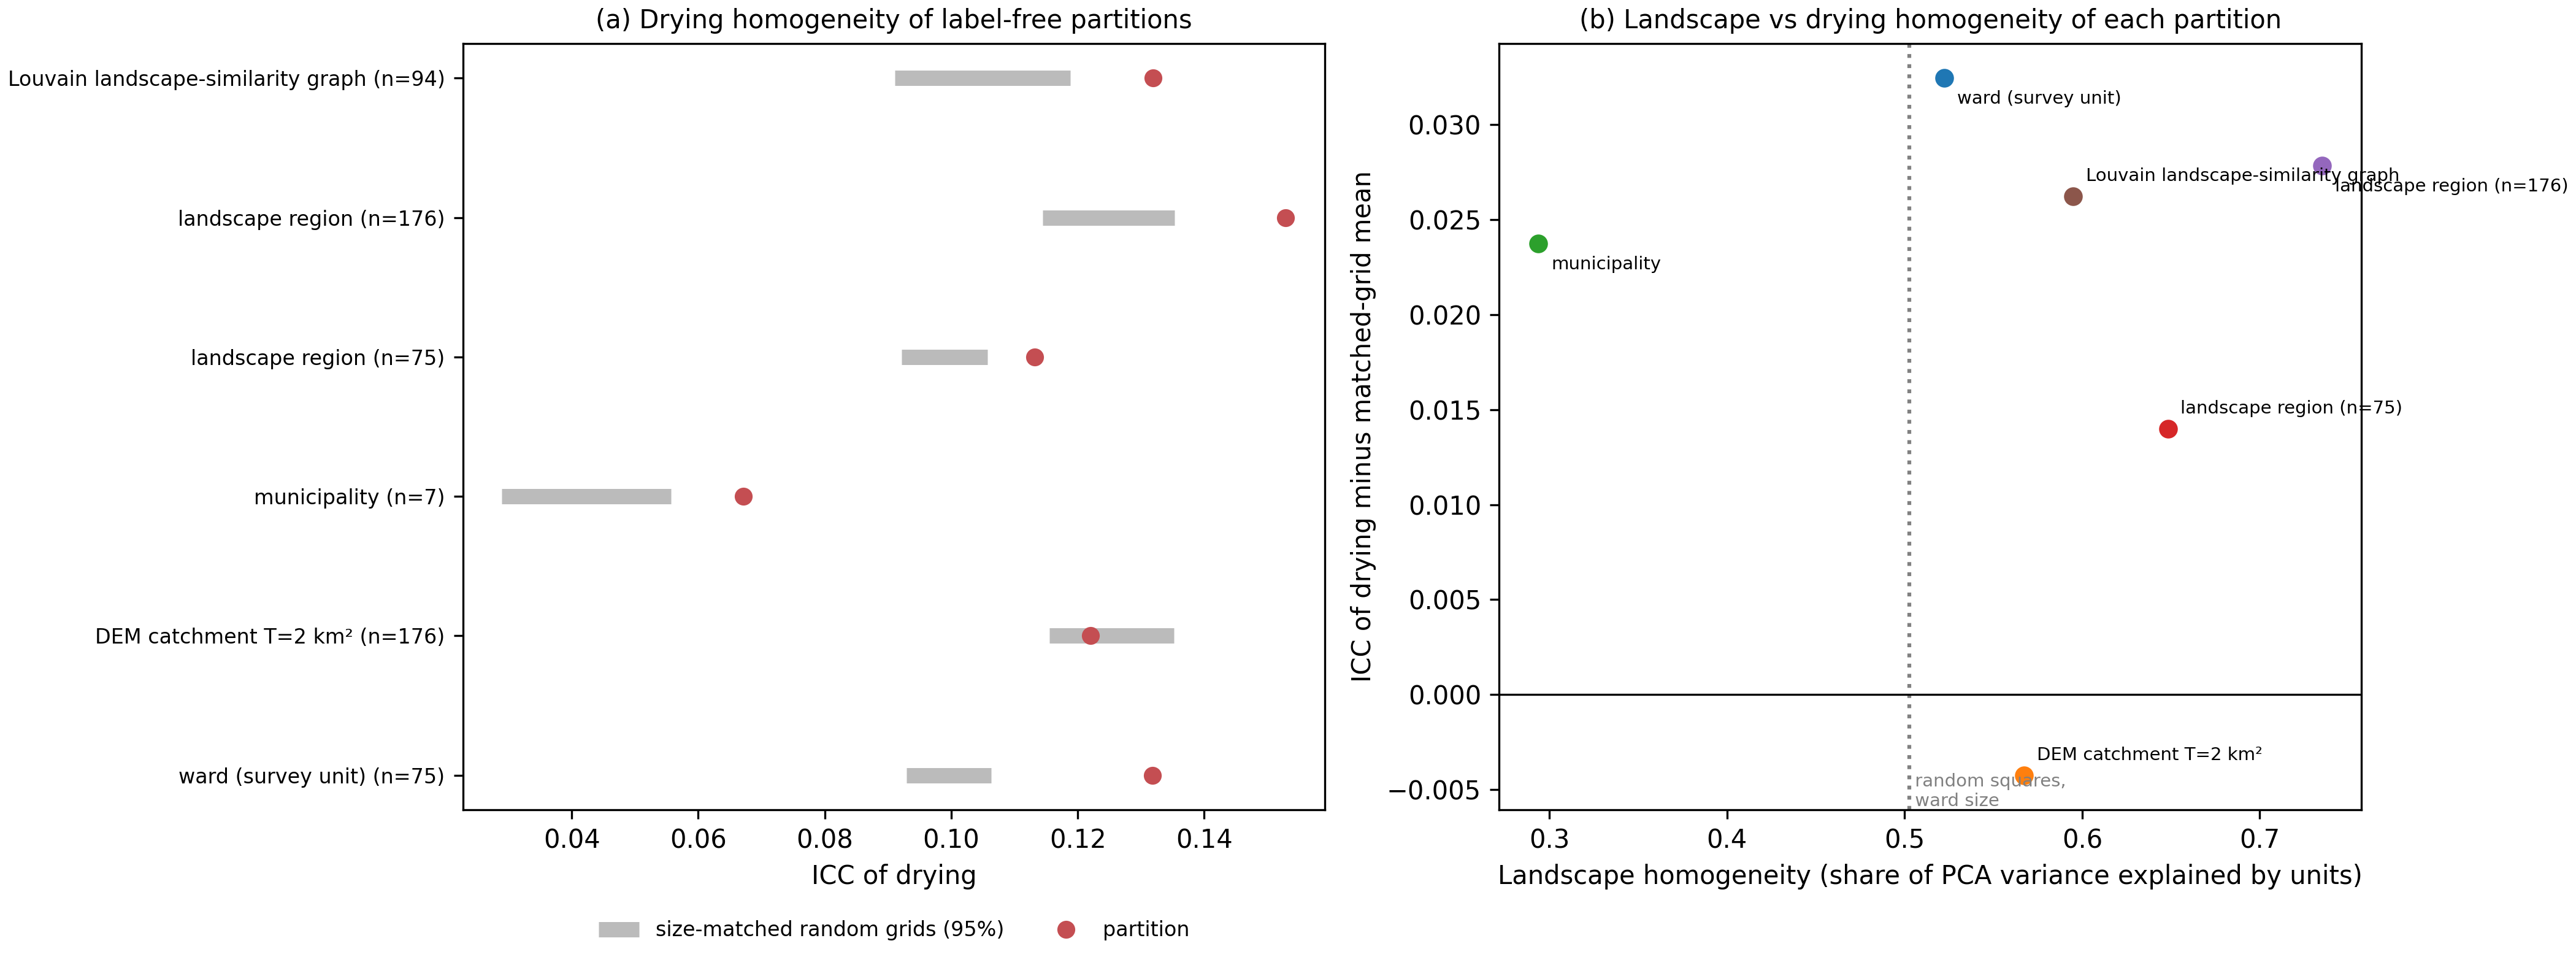
\includegraphics[width=0.64\linewidth]{un_regionalisation.png}
  \caption{(Left) Copernicus GLO-30 D8 drainage network and sources. (Right, a) ICC of drying for wards, municipalities, DEM catchments, landscape regions and landscape-similarity communities (red) against 200 size-matched random grids (grey, 95\% range). (Right, b) Landscape homogeneity against excess drying homogeneity; dotted line: random squares of ward size.}
  \label{fig:hydro}
\end{figure}

\begin{figure}[t]
  \centering
  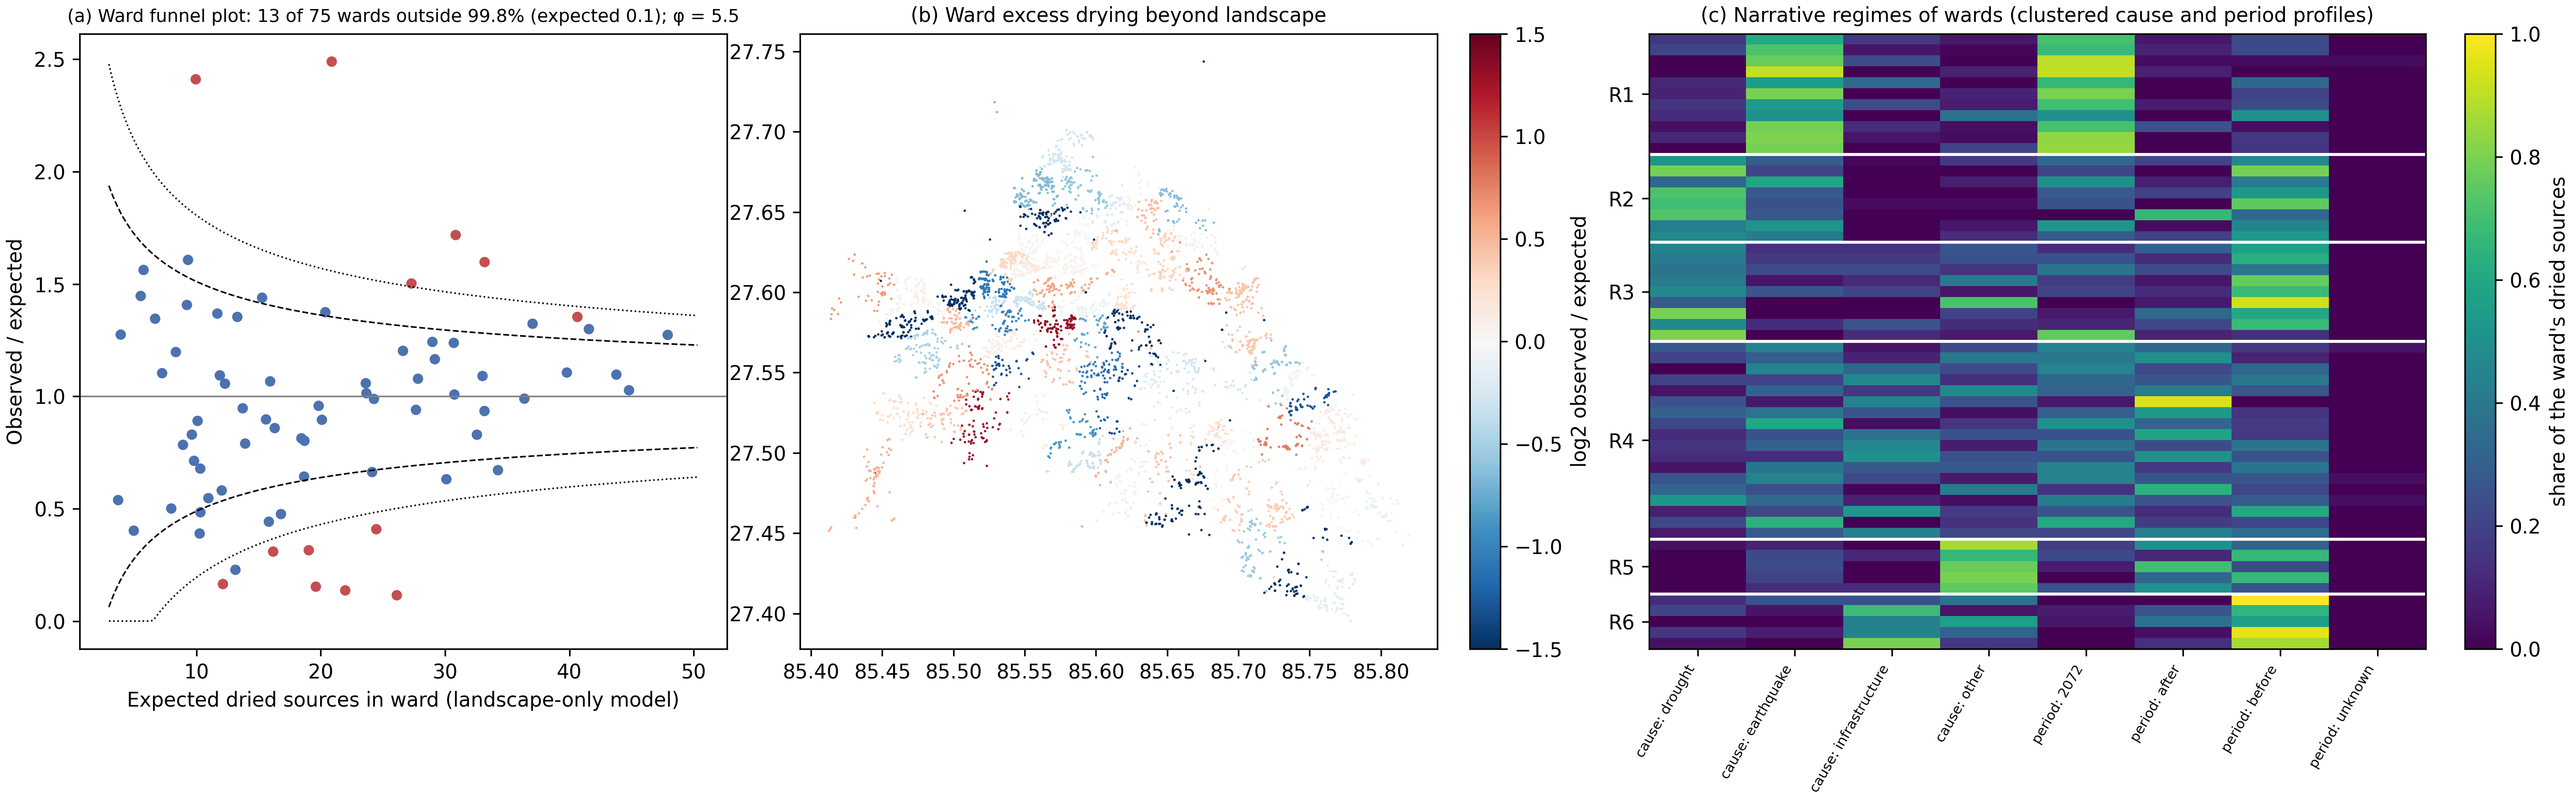
\includegraphics[width=\linewidth]{un_wards.png}
  \caption{Ward effects. (a) Funnel plot of observed/expected dried sources per ward against a landscape-only model (dashed: 95\%; dotted: 99.8\% limits; red: outside 99.8\%). (b) Map of ward excess. (c) Narrative regimes: wards (rows) clustered by the shares of reported causes and periods of their dried sources.}
  \label{fig:wards}
\end{figure}

\begin{table}[t]
  \centering
  \caption{Three-way variation partitioning of drying (adjusted McFadden pseudo-$R^2$) between environment ($E$; 65 covariates), space ($S$; 250 Moran eigenvector maps) and ward ($W$; 75 wards).}
  \label{tab:partition}
  \small
  \begin{tabular}{lclc}
    \toprule
    Fraction & pseudo-$R^2$ & Fraction & pseudo-$R^2$ \\
    \midrule
    Environment only & 0.050 & Environment $\cap$ space & 0.011 \\
    Ward only & 0.019 & Environment $\cap$ ward & 0.010 \\
    Space only & $-0.002$ & Space $\cap$ ward & 0.036 \\
    All three & 0.042 & Unexplained & 0.835 \\
    \bottomrule
  \end{tabular}
\end{table}

\subsection{Recalled causes and years are shared within wards}\label{sec:res-dried}
Respondents attribute drying mostly to the earthquake (34.3\%), drought (31.4\%) and infrastructure (15.8\%). 35.4\% of dried sources are dated to 2072~BS, 84.0\% of which are attributed to the earthquake, and reported years cluster on round numbers (Fig.~\ref{fig:timing}a; Tables~S35--S36).

\paragraph{Knox test.} Pairs within \SI{250}{\metre} report the same year 1.54 times as often as expected ($p = 0.001$). The excess is detected only for pairs within a ward (1.62, $p = 0.001$; 2,046 pairs). Across a ward boundary no excess was detected (0.72, $p = 0.83$), but there are only 196 such pairs. Without the 2072~BS cohort the contrast sharpens: 2.34 vs.\ 1.13 at \SI{250}{\metre} and 1.94 vs.\ 1.10 at \SI{1}{\kilo\metre} (Fig.~\ref{fig:mining}c; Table~S37).

\paragraph{Ward ICC of recalled attributes.} Within wards, the ICC exceeds every size-matched grid ($p = 0.005$; Fig.~\ref{fig:dried}; Table~S38):

\begin{center}
\small
\begin{tabular}{lcc}
  \toprule
  Recalled attribute & Ward ICC & Matched grids (95\% range) \\
  \midrule
  Earthquake attribution & 0.228 & 0.131--0.177 \\
  Drought attribution & 0.251 & 0.155--0.224 \\
  Infrastructure attribution & 0.264 & 0.152--0.208 \\
  Dating to 2072~BS & 0.280 & 0.111--0.178 \\
  \bottomrule
\end{tabular}
\end{center}

\noindent Within landscape types the ICC is 0.03--0.05, except for infrastructure (0.14), the one cause that follows the landscape (built-up settings).

\paragraph{Narrative rules.} The rules are strongly ward-robust (Table~S39). Dating to 2072~BS implies earthquake attribution (confidence 0.84; lift 2.45), reaching 0.94 in Temal and 0.90 in Panchkhal. Dating before 2072~BS implies drought (0.50; lift 1.60), reaching 0.78 in Temal.

\paragraph{Narrative regimes.} The 56 wards with at least eight dried sources form six regimes (Table~S42; Fig.~\ref{fig:wards}c), although the clustering is weak (silhouette 0.22; Table~S41):
\begin{itemize}
  \item 11 wards where 71\% of drying is attributed to the earthquake and 75\% dated to 2072~BS;
  \item wards dominated by drought before 2072~BS;
  \item infrastructure-dominated wards;
  \item wards citing other causes;
  \item mixed wards.
\end{itemize}
No association was detected between narrative similarity and the distance between wards (Mantel $r = -0.04$, $p = 0.79$), or between narrative similarity and landscape similarity ($r = 0.04$, $p = 0.25$), including in partial tests (Table~S43). With 56 wards, these tests can exclude only moderate correlations. The result is absence of evidence that neighbouring or landscape-similar wards tell similar stories, not evidence that narratives are independent of geography. Earthquake-attributed drying is also less predictable from environmental covariates than other drying (pooled out-of-fold \auc{} 0.650 [0.623, 0.674] vs.\ 0.712 [0.696, 0.730]; Table~S47).

\begin{figure}[t]
  \centering
  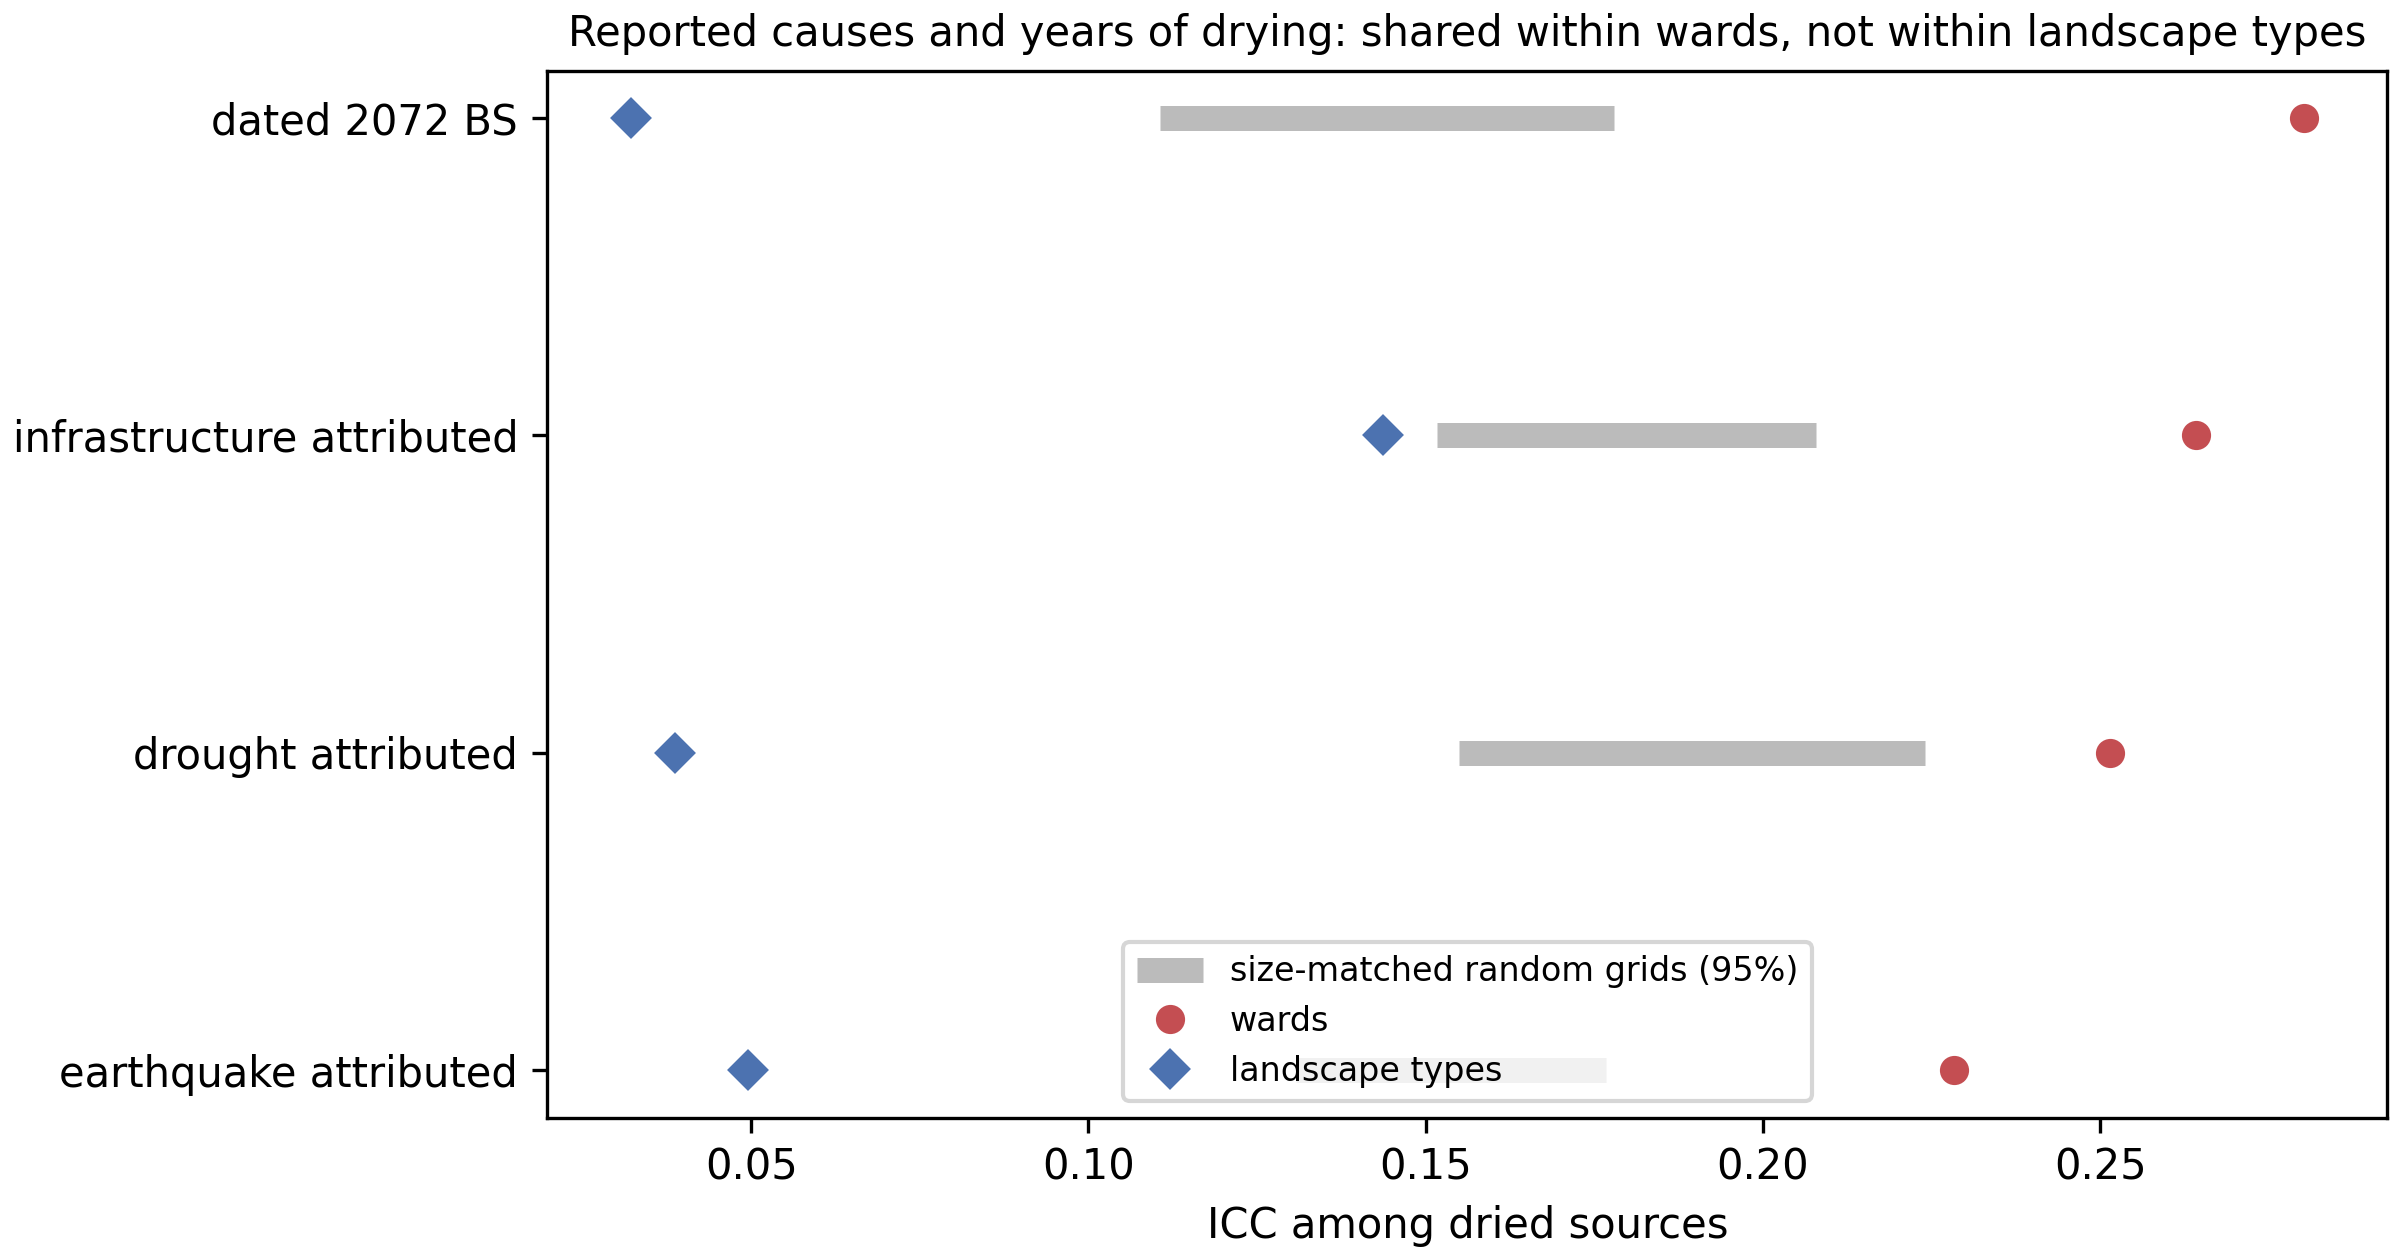
\includegraphics[width=0.72\linewidth]{un_dried_mining.png}
  \caption{ICC of recalled attributes among 1,521 dried sources within wards (red) and within landscape types (blue), against 200 size-matched random grids (grey, 95\% range).}
  \label{fig:dried}
\end{figure}

\begin{figure}[t]
  \centering
  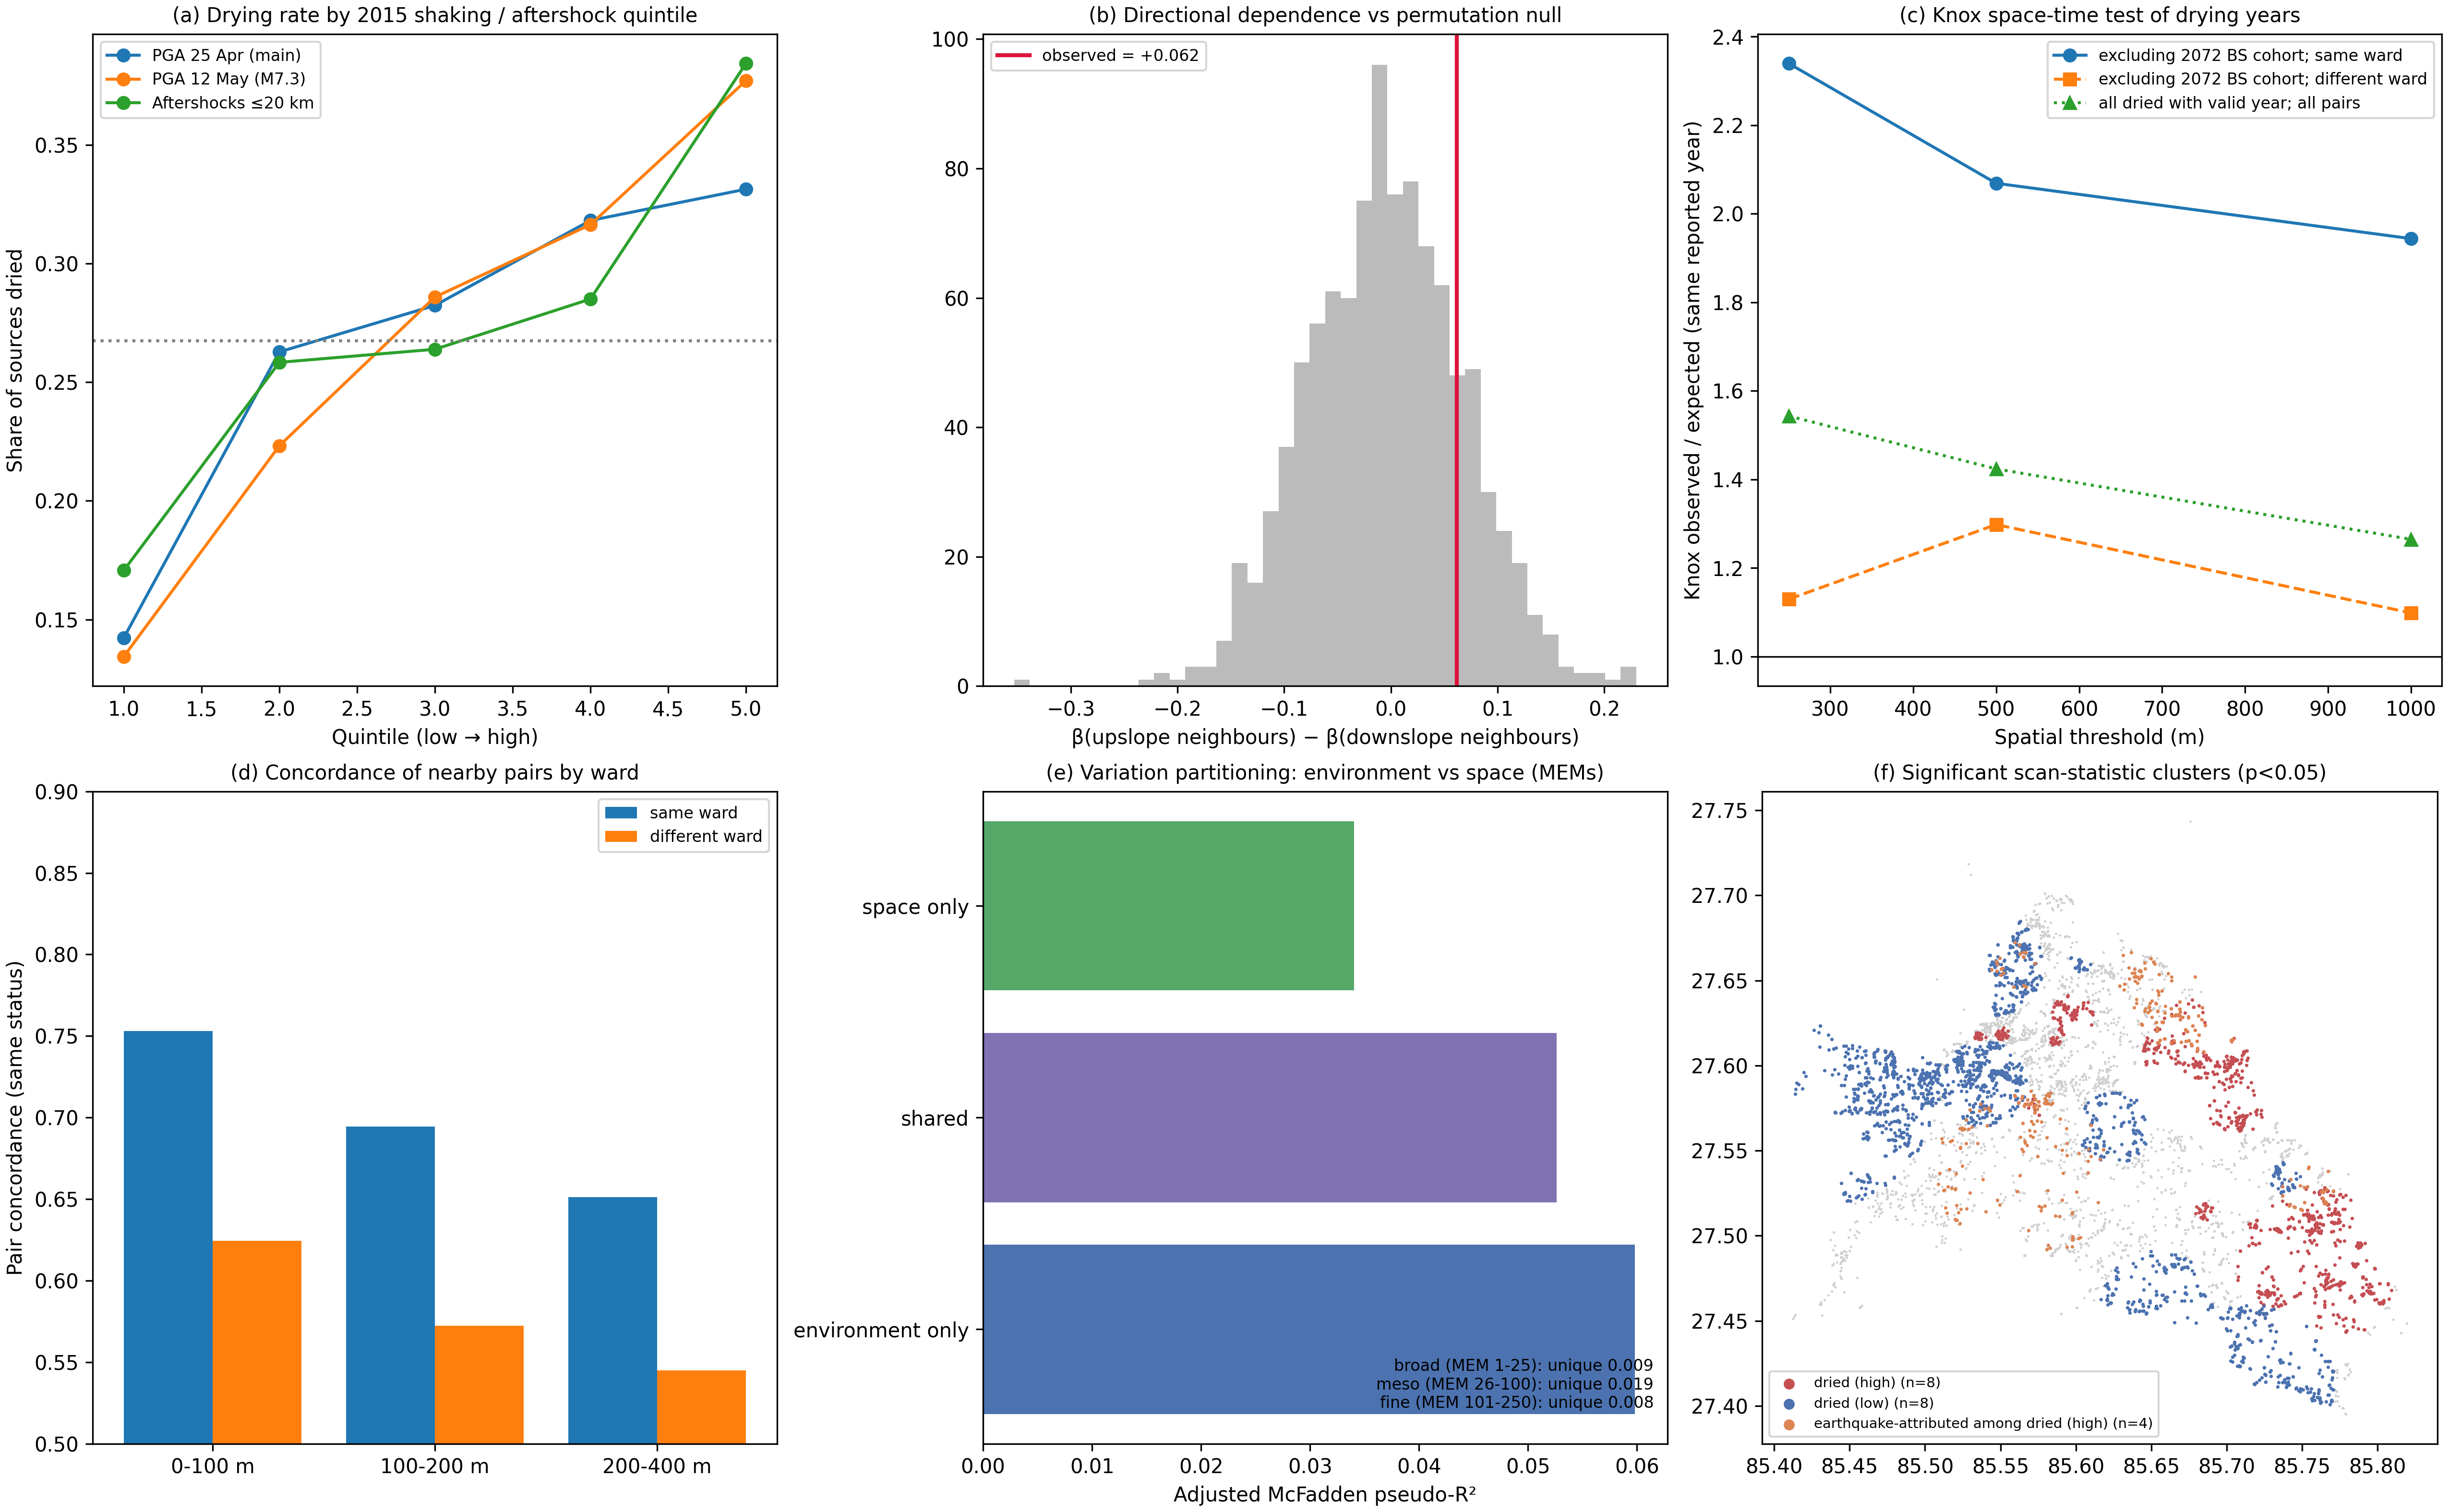
\includegraphics[width=\linewidth]{sa_spatial_data_mining.png}
  \caption{(a) Drying by quintile of 2015 shaking and aftershock count. (b) Upslope minus downslope neighbour effect against its permutation null. (c) Knox ratio of same-year pairs within and across wards. (d) Concordance of nearby pairs within and across wards. (e) Environment--space variation partitioning. (f) Significant scan-statistic clusters.}
  \label{fig:mining}
\end{figure}

\subsection{Drivers within wards}
With ward fixed effects and all 65 environmental covariates (Fig.~\ref{fig:drivers}; Table~S44), drying remains associated with:
\begin{itemize}
  \item higher topographic position: TPI $+0.23$ per SD [0.05, 0.43]; ALOS slope position $+0.24$ [0.10, 0.41];
  \item higher heat load: CHILI $+0.16$ [0.05, 0.28];
  \item fewer agricultural ($-0.67$) and dense-forest ($-0.59$) surroundings.
\end{itemize}
Associations with road density and NDVI that appeared with the base layers lose precision once land cover and built-up fraction enter. Soil moisture, soil texture and multi-scale TPI are associated pooled but are not identified within wards.

\begin{figure}[t]
  \centering
  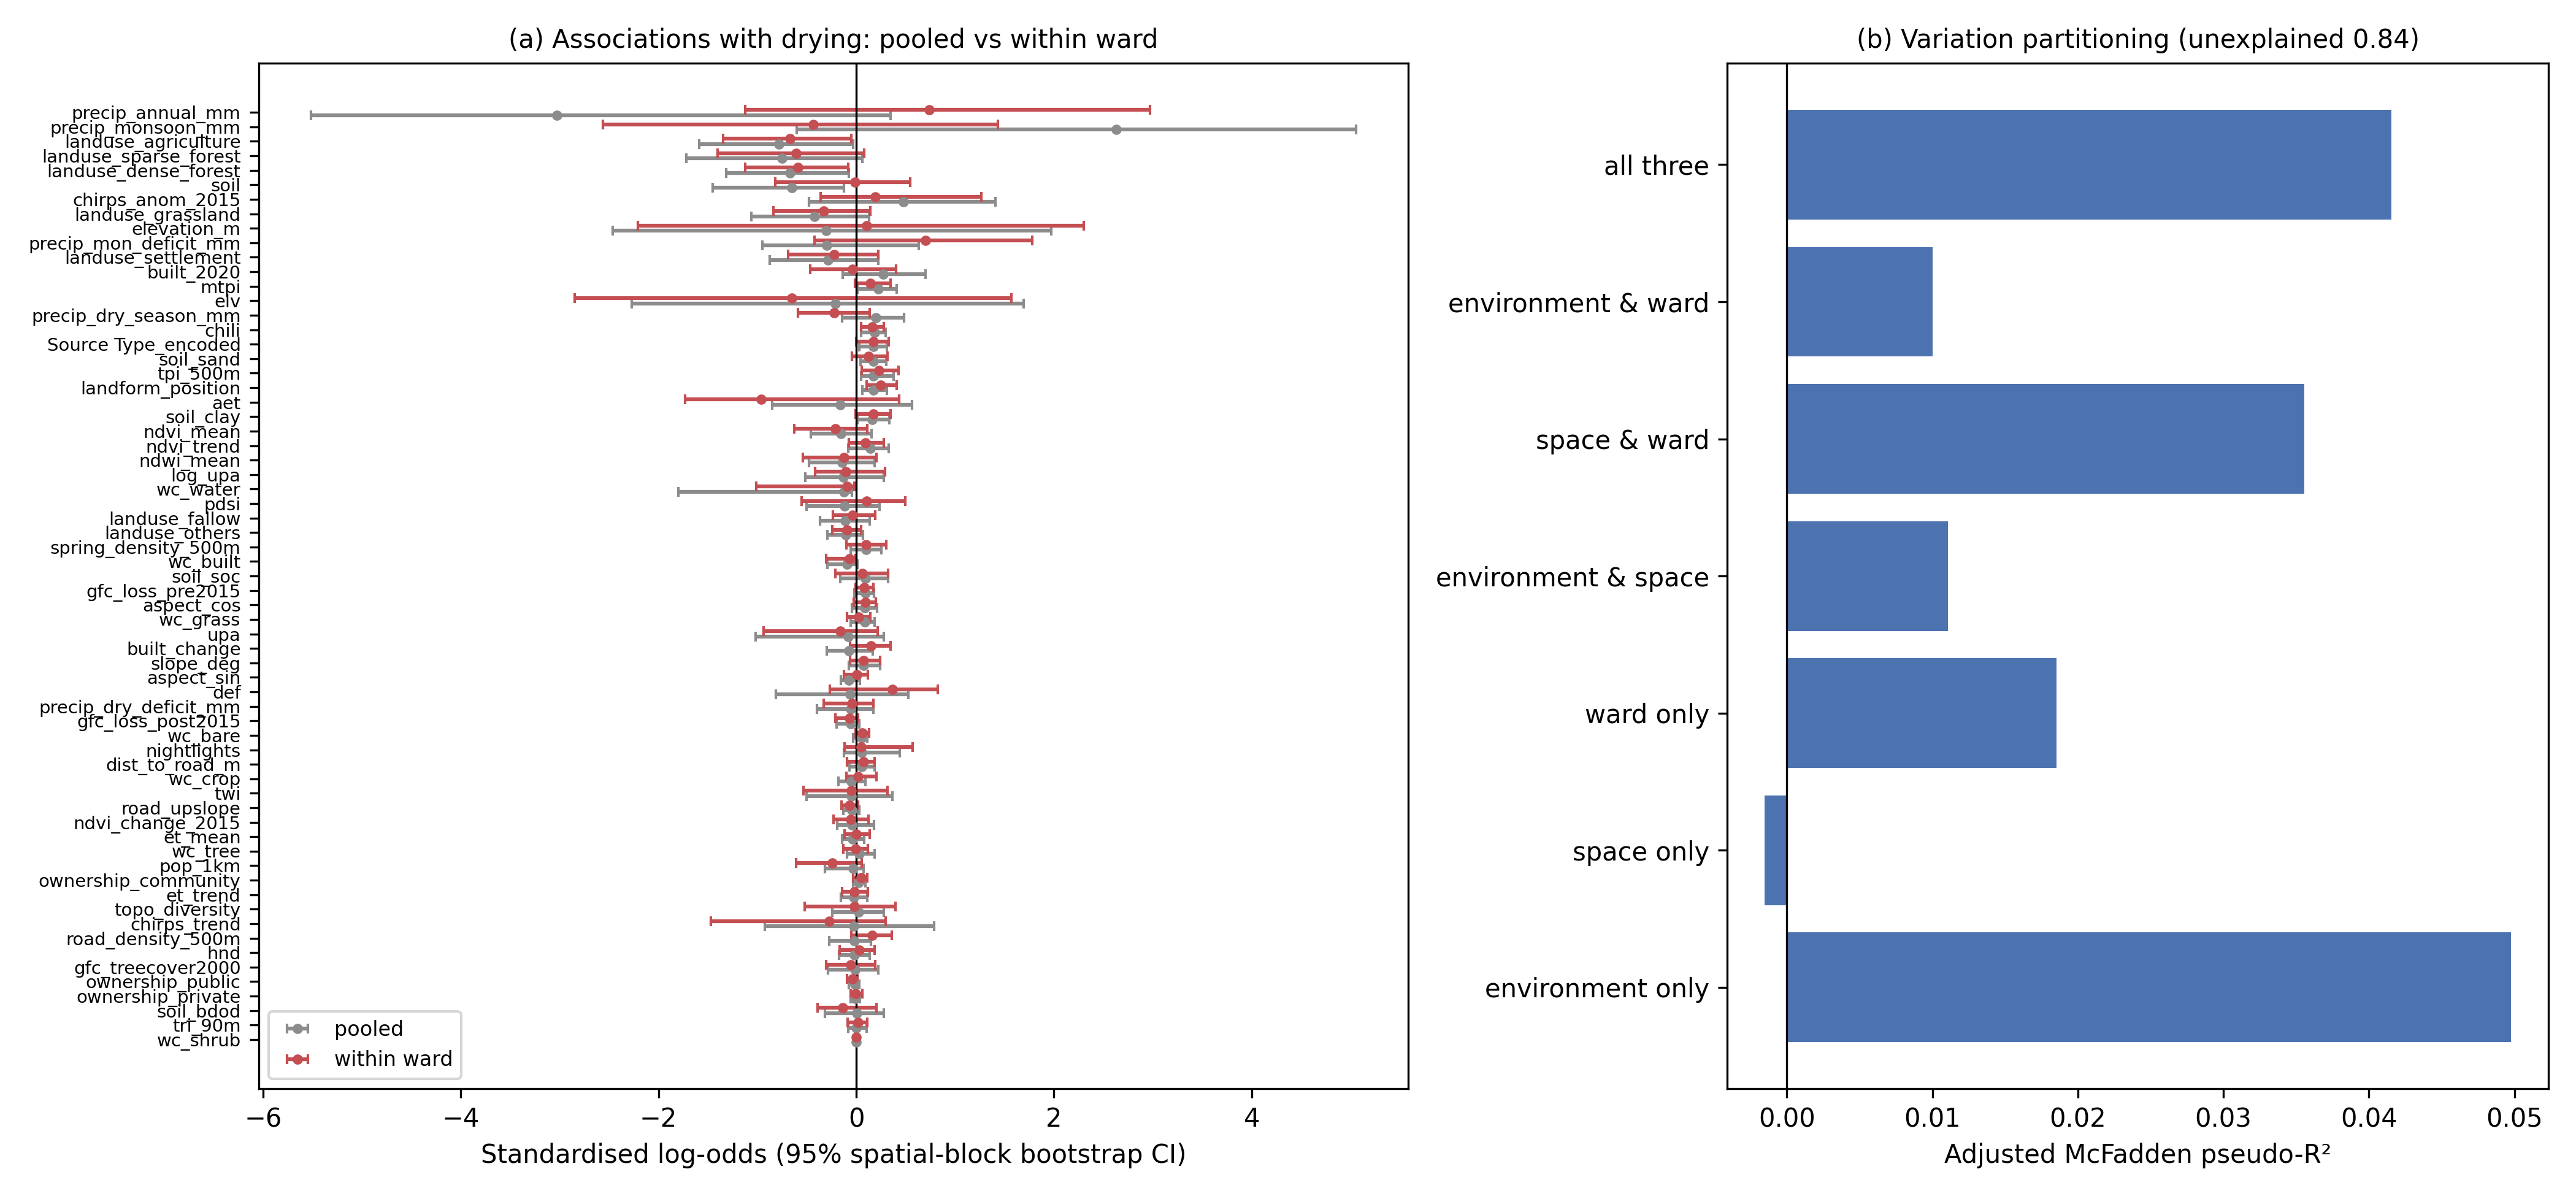
\includegraphics[width=\linewidth]{dr_drivers.png}
  \caption{(a) Standardised log-odds of drying, pooled (grey) and with ward fixed effects (red), with 95\% spatial-block bootstrap intervals. (b) Three-way variation partitioning.}
  \label{fig:drivers}
\end{figure}

\subsection{Earthquake shaking}
Drying rises across quintiles of every exposure measure (Fig.~\ref{fig:mining}a; Table~S45):
\begin{itemize}
  \item mainshock PGA: 14.2\% to 33.1\%;
  \item 12 May PGA: 13.4\% to 37.7\%;
  \item aftershock count: 17.1\% to 38.4\%.
\end{itemize}
The measures are collinear and are not identified jointly without adjustment. With environmental adjustment, 12 May PGA remains associated with drying (0.69 per SD; 0.24--1.03), and the association persists with 100 Moran eigenvector maps added (0.74; 0.37--1.04; Table~S55). With ward fixed effects it is attenuated and no longer distinguishable from zero (0.35; $-0.10$ to 0.78). This model is weakly informative, because only 11\% of the variance of either PGA field and 7\% of the aftershock count lies within wards (Table~S54). Shaking and ward are largely confounded at this scale. The data can neither confirm nor exclude an effect of shaking that varies within wards. Among dried sources, no exposure measure predicts earthquake attribution or dating to 2072~BS.

\begin{figure}[t]
  \centering
  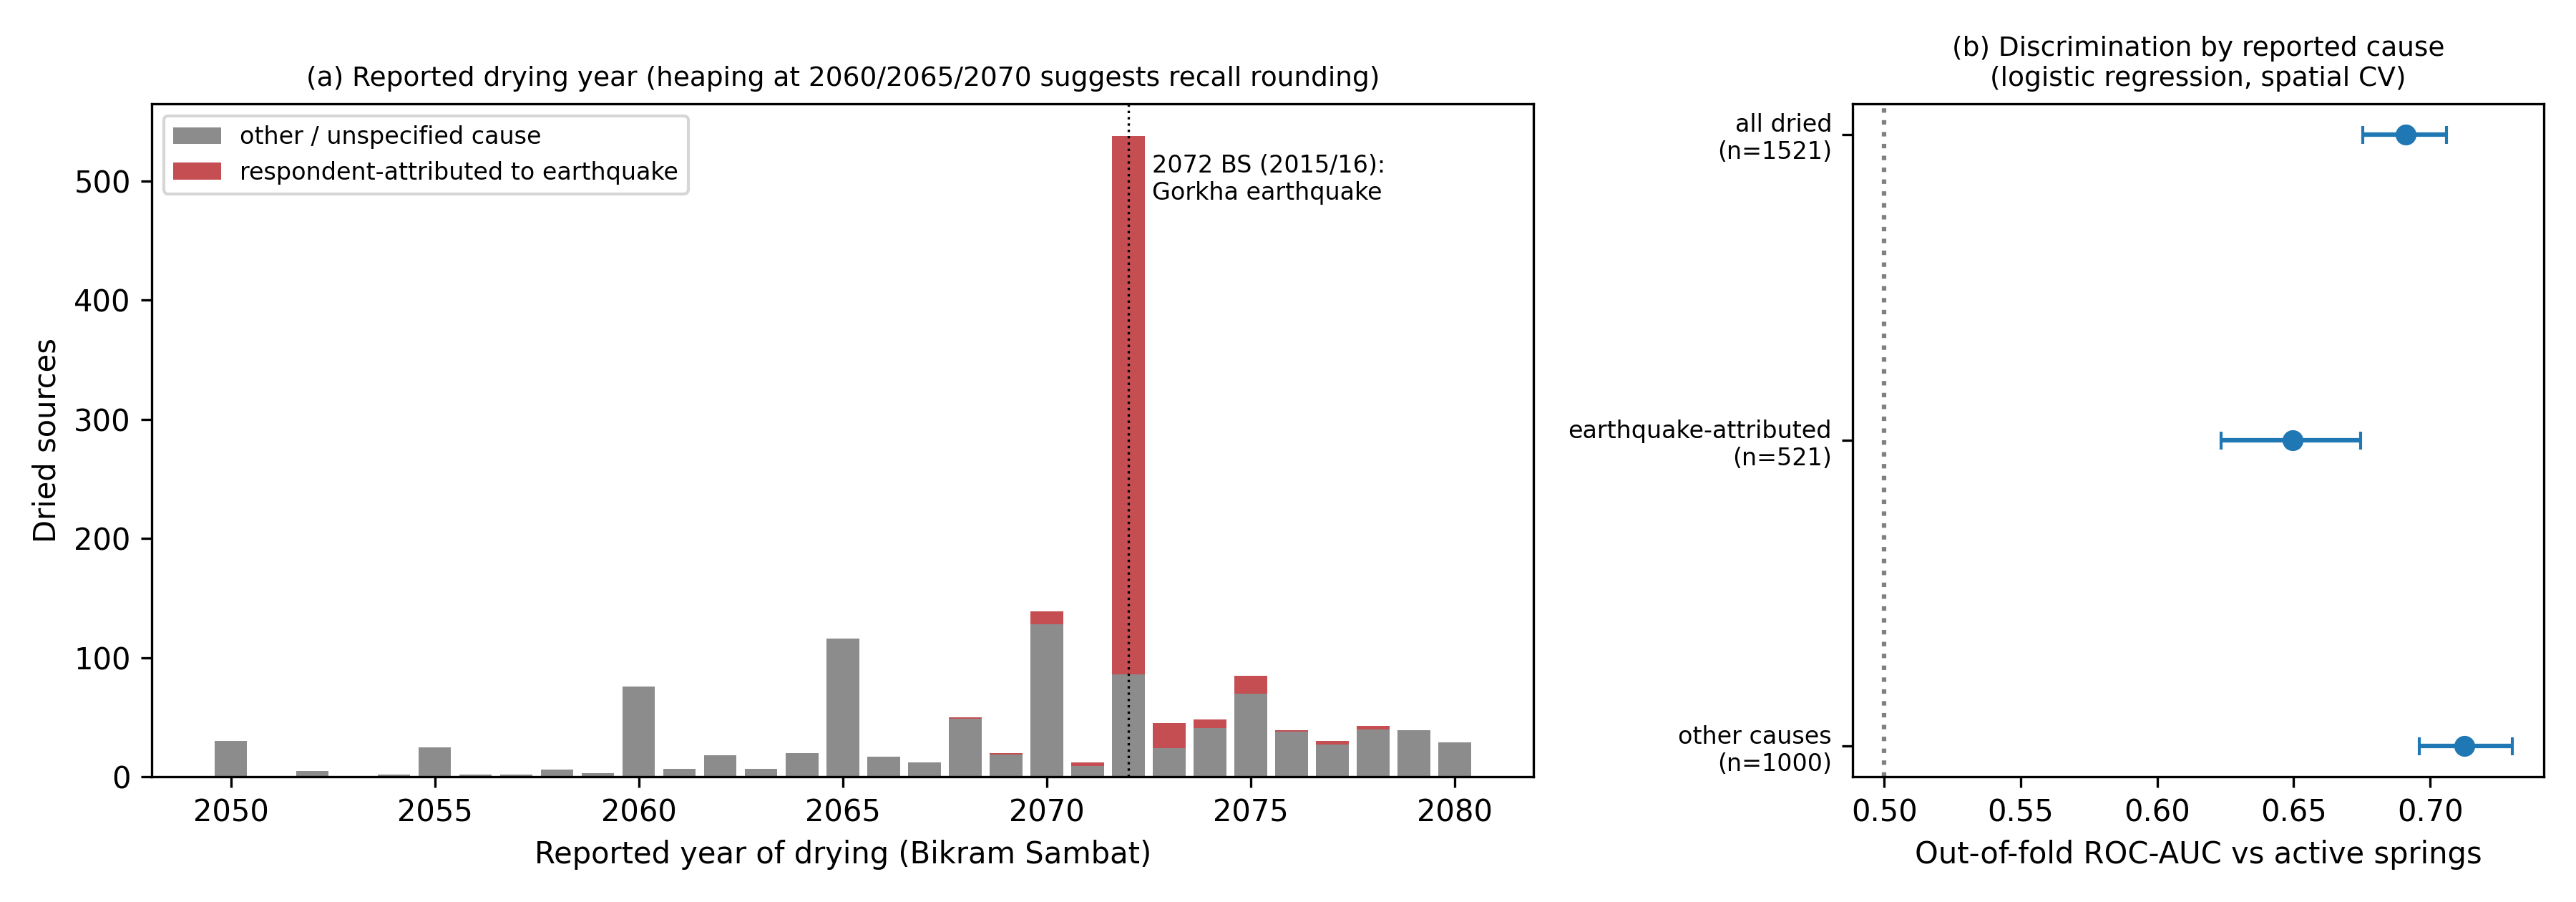
\includegraphics[width=\linewidth]{drying_timing_and_cause.png}
  \caption{(a) Reported year of drying (Bikram Sambat) by reported cause; 2072~BS spans April 2015--April 2016. (b) Pooled out-of-fold \auc{} for earthquake-attributed and other dried sources against active sources (95\% bootstrap CI).}
  \label{fig:timing}
\end{figure}

\subsection{Sensitivity to ponds, seasonal sources and the null partition}\label{sec:res-sens}
Table~\ref{tab:sens} repeats the ward analyses after excluding ponds, seasonal sources or both.
\begin{itemize}
  \item \textbf{Ward signal.} The ward signal does not depend on these groups. It strengthens when seasonal sources are removed, from ICC 0.132 to 0.185 for perennial springs, and stays above both null partitions in every subset.
  \item \textbf{Funnel and recalled attributes.} Overdispersion stays at 5.3--6.3, and 11--15 wards lie outside 99.8\% limits. The ward ICC of earthquake attribution and of dating to 2072~BS exceeds both nulls in every subset.
  \item \textbf{Knox test.} Same-ward Knox clustering persists (ratio 1.62--1.91, $p = 0.001$). Across ward boundaries the ratio rises above 1 in the subsets (1.19--1.45) but is not significant on 25--63 pairs. This contrast should therefore be read as suggestive rather than decisive.
  \item \textbf{Rules.} The two headline rules are stable. ``TPI high'' has a within-ward OR of 1.85--2.34, and ``TPI low \& soil moisture high'' 0.17--0.26 for drying.
  \item \textbf{Catchments.} DEM catchments remain no better than grids.
  \item \textbf{Landscape regions.} The advantage of the 75 label-free landscape regions over grids is \emph{not} robust. It disappears when seasonal sources are excluded ($p = 0.25$--0.31). Part of the landscape-region signal in the full data thus comes from where seasonal sources are, while the ward signal does not.
\end{itemize}
The landscape-type contrast persists (7--29\% drying for perennial springs).

\begin{table}[t]
  \centering
  \caption{Sensitivity of the ward analyses to the definition of the population (Table~S52). Null partitions: 200 size-matched grids and 200 sets of contiguous random regions with the ward size distribution. In every subset the ward ICC of drying exceeds all 200 members of both nulls ($p = 0.005$, the minimum attainable). Knox ratios are for same-year pairs within \SI{250}{\metre}.}
  \label{tab:sens}
  \small
  \begin{tabular}{lcccc}
    \toprule
     & All sources & Springs only & Perennial only & Perennial springs \\
    \midrule
    Sources (dried) & 5,689 (1,521) & 5,168 (1,264) & 4,759 (934) & 4,477 (835) \\
    Ward ICC & 0.132 & 0.140 & 0.170 & 0.185 \\
    \quad grids, 97.5th percentile & 0.106 & 0.109 & 0.121 & 0.135 \\
    \quad random regions, 97.5th percentile & 0.111 & 0.112 & 0.126 & 0.138 \\
    Catchment (\SI{2}{\kilo\metre\squared}) ICC vs.\ grid $p$ & 0.75 & 0.81 & 0.48 & 0.55 \\
    Landscape regions (75) vs.\ grid $p$ & 0.010 & 0.030 & 0.31 & 0.25 \\
    Funnel $\phi$ (wards outside 99.8\%) & 5.5 (13) & 5.3 (11) & 6.3 (15) & 5.9 (13) \\
    Knox within wards (pairs) & 1.62 (2,046) & 1.68 (1,310) & 1.91 (964) & 1.84 (763) \\
    Knox across wards (pairs) & 0.72 (196) & 1.21 (63) & 1.19 (59) & 1.45 (25) \\
    Ward ICC, earthquake attribution & 0.228 & 0.232 & 0.249 & 0.233 \\
    Ward ICC, dated 2072~BS & 0.280 & 0.276 & 0.269 & 0.253 \\
    MH OR, TPI high $\rightarrow$ dried & 2.27 & 1.85 & 2.34 & 1.96 \\
    \bottomrule
  \end{tabular}
\end{table}

\begin{figure}[t]
  \centering
  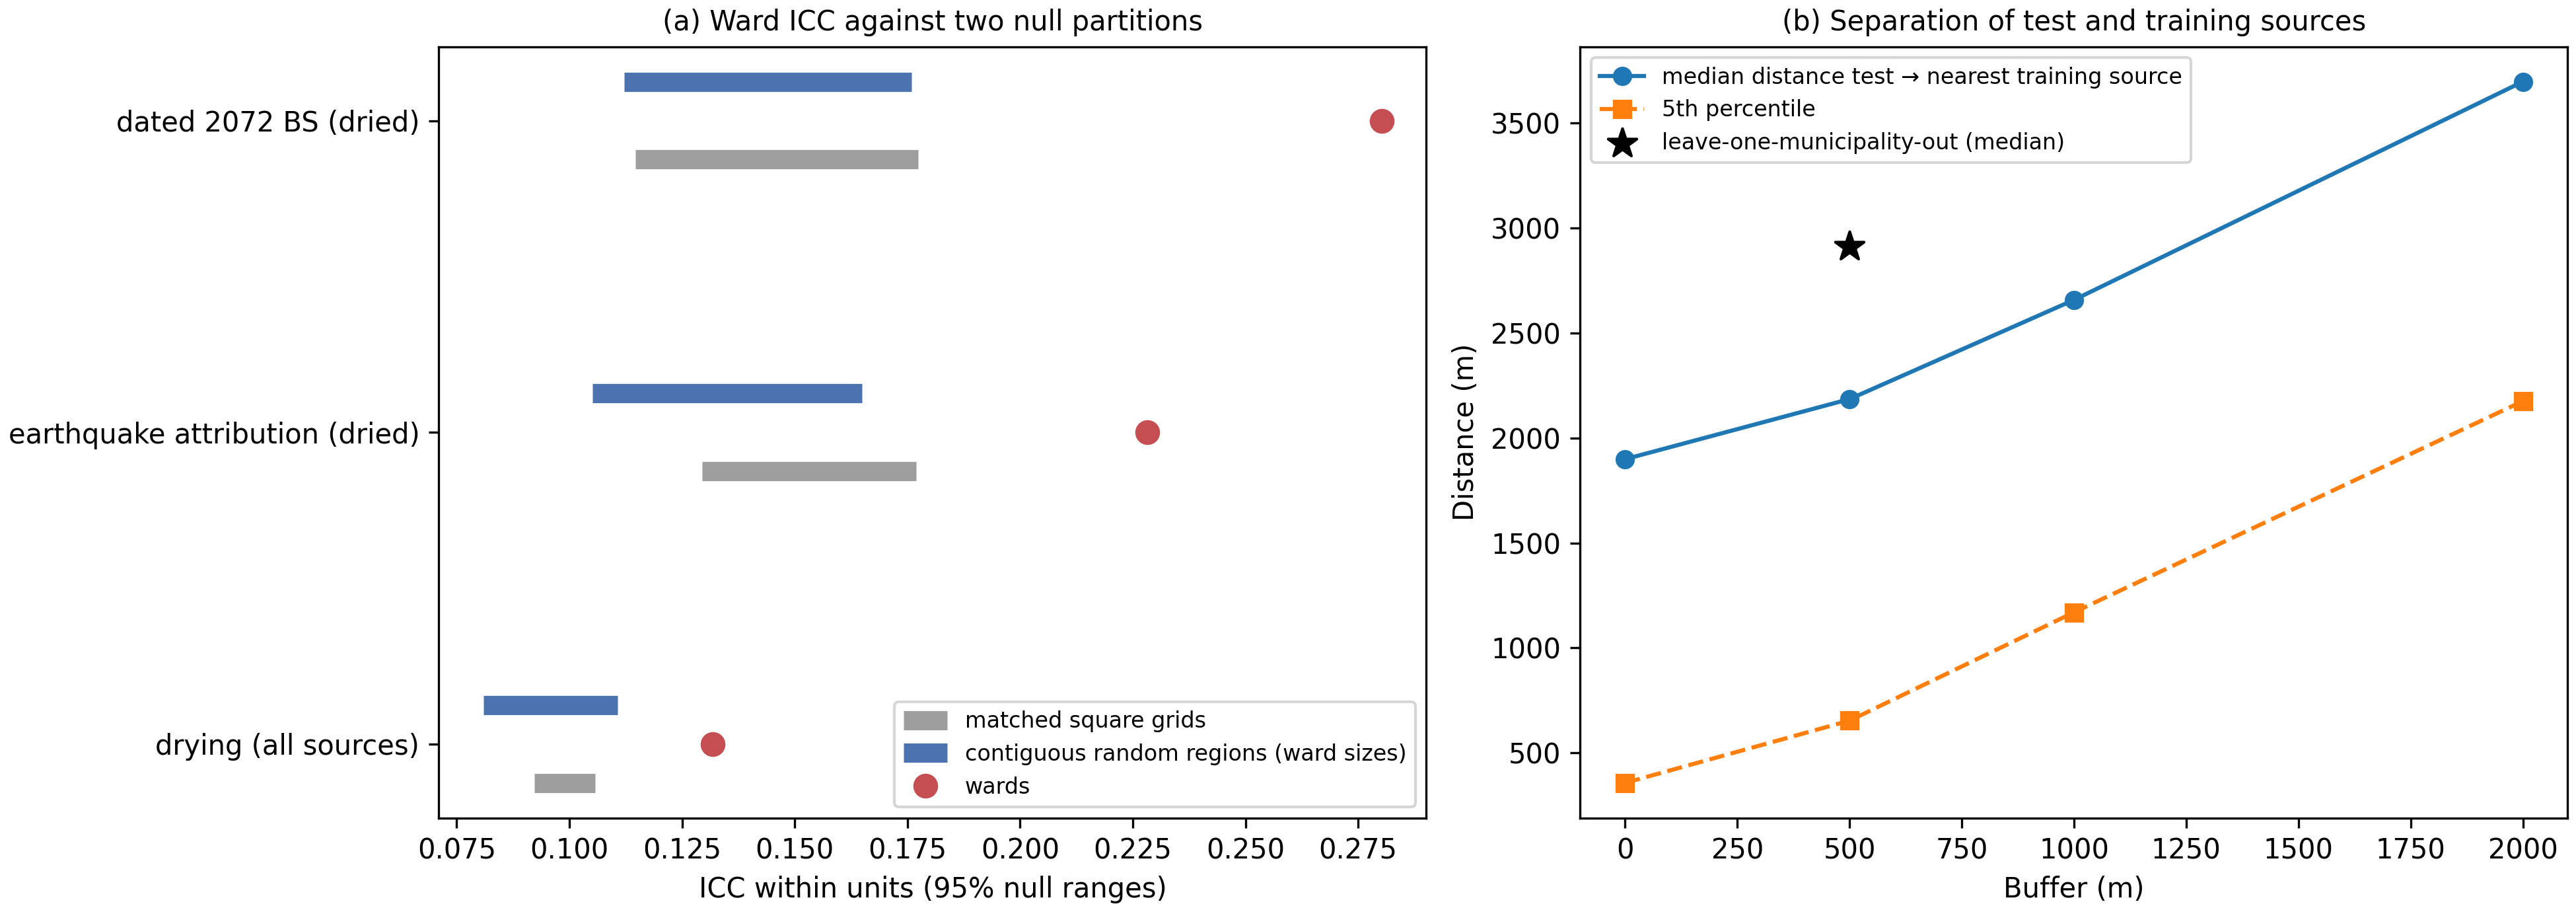
\includegraphics[width=\linewidth]{rb_robustness.png}
  \caption{(a) Ward ICC of drying and of two recalled attributes (red) against 95\% ranges of size-matched square grids (grey) and contiguous random regions with the ward size distribution (blue). (b) Distance from test sources to the nearest training source under spatial block cross-validation with increasing buffers, and for leave-one-municipality-out.}
  \label{fig:robust}
\end{figure}

\subsection{No graph topology carries information}
All four geographic graphs join same-status sources to the same degree (label assortativity $\kappa = 0.22$--0.23), whether built from proximity, catchments, ridge-aware costs or wards; random links give $\kappa = 0.00$ (Table~S48). No topology improves GraphSAGE or the residual GATv2 over the graph-free MLP ($\Delta$\auc{} $-0.017$ to $+0.004$, all intervals spanning zero), and random links perform as well as any graph (Fig.~\ref{fig:topology}; Tables~S49--S50). Placebo edge attributes and topologies likewise leave accuracy unchanged (Table~S7).

\begin{figure}[t]
  \centering
  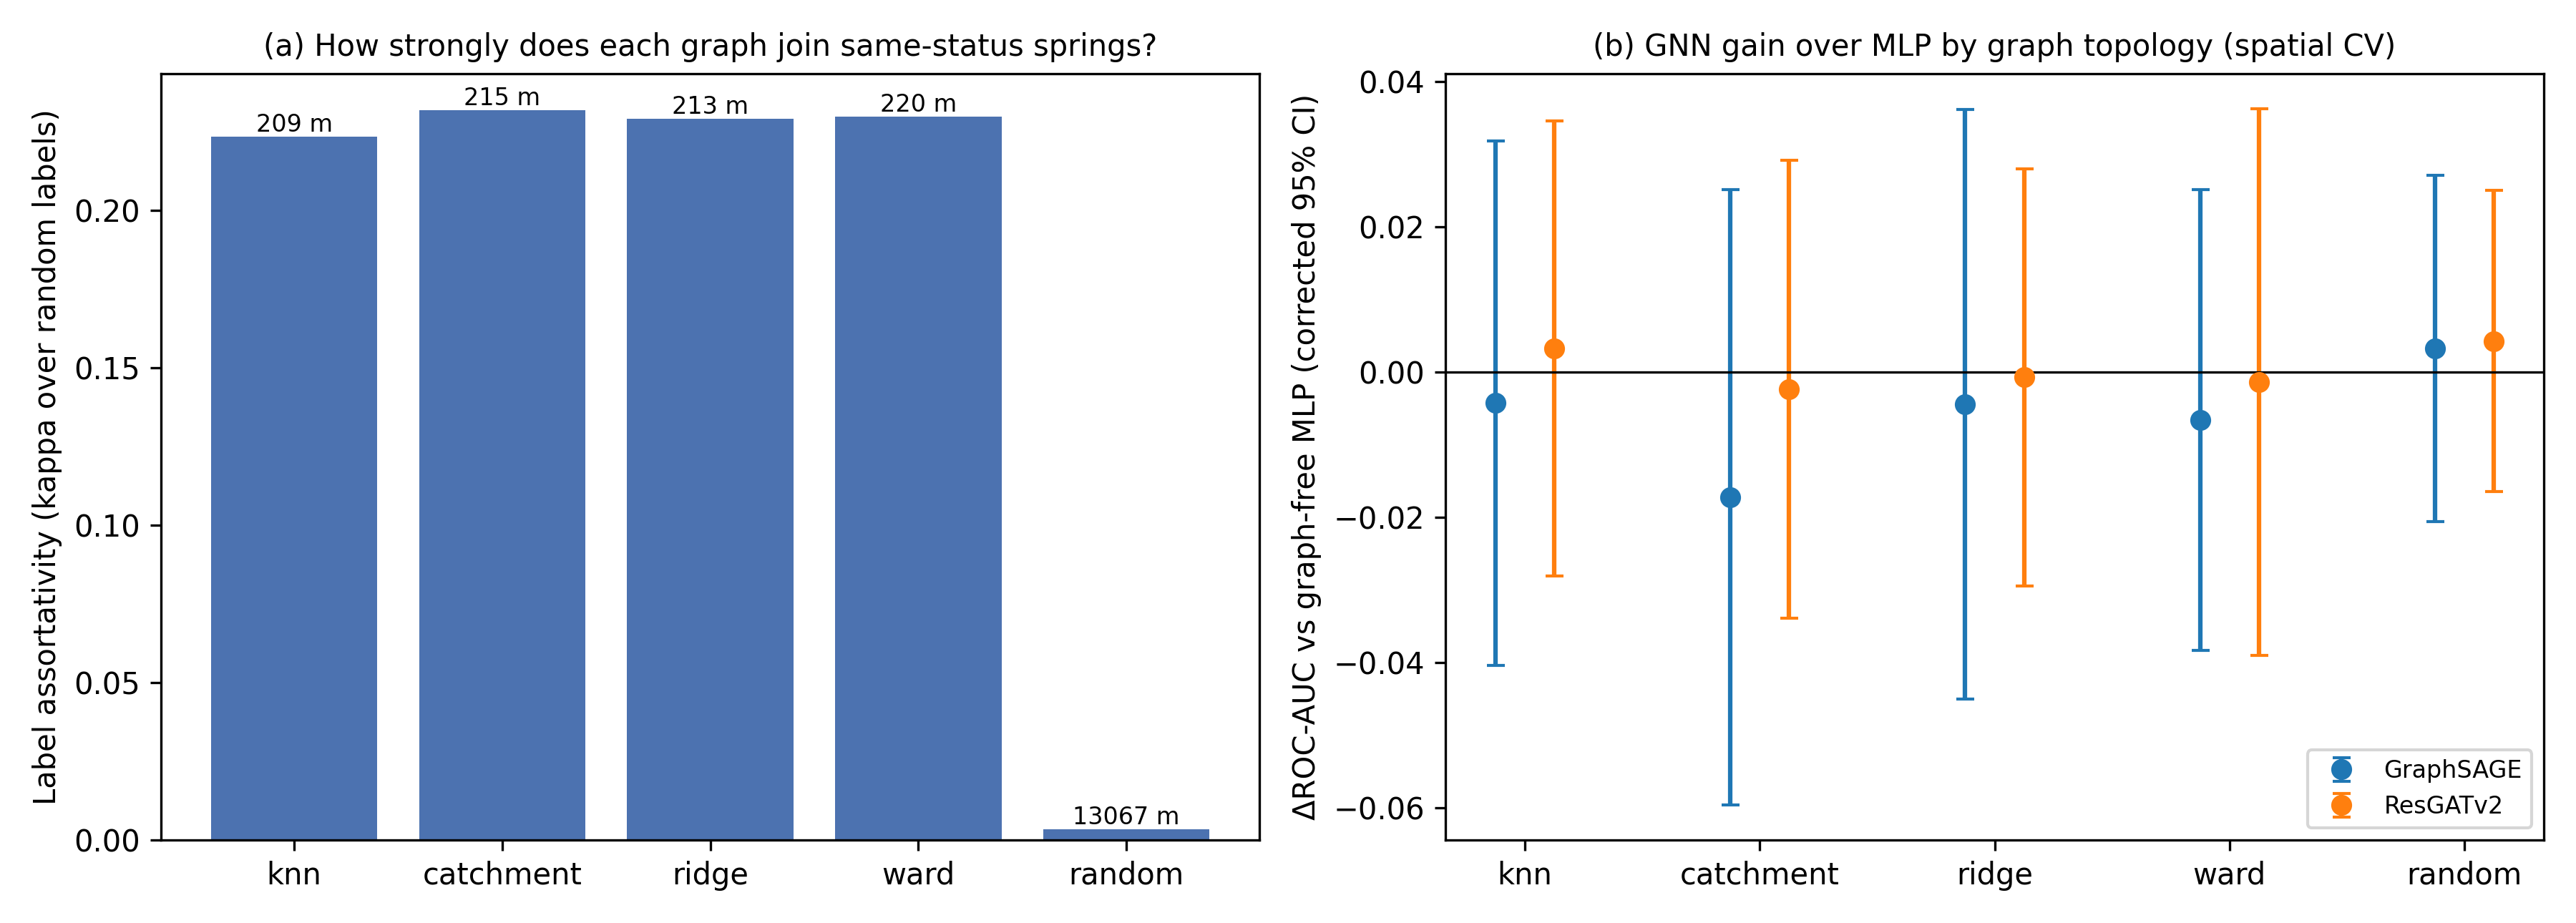
\includegraphics[width=\linewidth]{gt_topology.png}
  \caption{(a) Label assortativity and median edge length of five spring graphs. (b) \auc{} gain of GraphSAGE and a residual GATv2 over a graph-free MLP on each graph (spatial CV, $5 \times 5$; corrected 95\% CI).}
  \label{fig:topology}
\end{figure}

% =============================================================================
\section{Discussion}\label{sec:discussion}

\subsection{Two kinds of structure}
The inventory contains two kinds of spatial structure.

\paragraph{Landscape.} Landscape structure is visible to every unsupervised method that ignores labels and survey fields. Landscape types differ threefold in drying, also among perennial springs. Landscape regions are more homogeneous than chance in the full data, although not once seasonal sources are excluded. Most apriori rules---dominated by topographic position, height above drainage and water balance---hold within wards and replicate across spatial blocks. The riskiest settings are built-up, peri-urban surroundings and steep, water-limited slopes high above drainage. The safest are wet, forested uplands and low, moist positions.

\paragraph{Wards.} The second structure follows wards. Wards are not landscape units---they are no more landscape-homogeneous than random squares---yet they are as homogeneous in drying as the best landscape partition. They exceed both size-matched grids and contiguous random regions of ward size. They are strongly overdispersed against a landscape model and account for almost all purely spatial variation. Recalled narratives are shared within them, and no sharing was detected across their boundaries. All of this holds when ponds and seasonal sources are excluded. In the tests of Table~\ref{tab:predictions} in which the two explanations disagree, the outcomes agree with the survey-process explanation.

\paragraph{What the ward signal is, and is not.} \emph{The data demonstrate ward-level structure. They suggest, but do not prove, that collection practices produced it.} The inventory contains no enumerator identifier or visit date, so a ward effect cannot be resolved into its candidate causes:
\begin{itemize}
  \item survey process: classification of marginal sources and elicitation of dates and causes by the resource persons who covered a ward;
  \item visit season, which may differ between wards;
  \item real ward-level differences in water supply schemes, abstraction, road building and land management, which are organised by the same administrative units.
\end{itemize}
Physical ward-level change alone would not readily explain three observations, which therefore make survey process a plausible contributor:
\begin{itemize}
  \item Recalled \emph{dates} and \emph{causes} exceed their size-matched nulls by wider margins than drying itself. They are shared barely at all within landscape types and are not predicted by measured shaking.
  \item Same-year clustering is detected within wards but not across their boundaries.
  \item No geographic or landscape structure was detected in narrative similarity.
\end{itemize}
Each of these is weaker than it may appear. The cross-boundary Knox test has few pairs, and its ratio exceeds 1 in some subsets. The Mantel tests have limited power with 56 wards. Recalled narratives can also be shared through community discussion within a ward, independently of enumerators. We therefore describe the result as ward-associated heterogeneity consistent with survey-process effects. Attributing it to observers requires enumerator and date metadata, or a re-survey with crossed teams (Sect.~\ref{sec:recs}).

\subsection{Why watersheds do not organise drying}
DEM catchments were no more homogeneous than squares, status did not propagate along slope, flow-path covariates were uninformative after adjustment, and catchment- and ridge-aware graphs were no more label-assortative than proximity graphs. Mid-Hill springs are fed by fractured and weathered-rock aquifers whose recharge areas are set by lithology and fractures and need not coincide with topographic catchments \citep{thapa2023recharge}. A \SI{30}{\metre} surface model resolves surface drainage but not groundwater divides. Position within the landscape, by contrast, matters at every scale examined:
\begin{itemize}
  \item TPI, multi-scale TPI and ALOS slope position in the rules;
  \item TPI and slope position within wards;
  \item the slope-position axis of the PCA.
\end{itemize}
This is consistent with small, shallow local recharge areas near spurs and ridges responding first to reduced recharge.

\subsection{Human footprint and the 2015 earthquake}
\paragraph{Human footprint.} The peri-urban landscape type dries most, and it is the only setting in which a recalled cause (infrastructure) follows the landscape. This agrees with national evidence that roads and infrastructure are a leading cause of drying \citep{thapa2023drying, pandit2024depleting}. Individual footprint covariates are, however, collinear, and road density loses precision once land cover enters.

\paragraph{The earthquake.} All earthquake results are associations in a single cross-section with no pre-2015 status. Drying is more common where 2015 shaking was stronger, and the association with 12 May PGA survives environmental and broad-scale spatial (MEM) adjustment. It does not survive ward fixed effects. Because 89\% of the PGA variance lies between wards, this attenuation is uninformative: ward adjustment removes nearly all exposure contrast, together with any ward-level survey or management differences. An effect of shaking is plausible given observations in Melamchi \citep{chapagain2019status} and seismically induced permeability change \citep{wang2010earthquakes, manga2012changes}. It cannot be separated here from the eastward regional gradient, from ward effects or from the regional drying clusters. Shaking also does not predict which dried sources are attributed to, or dated to, 2015. Attribution and dating are the most ward-shared attributes in the inventory. The data are therefore compatible both with a physical effect of shaking and with the earthquake serving as a salient, locally shared explanation for drying that occurred over a longer period. Separating them would need sources with pre-2015 records or a design with exposure contrast within wards.

\subsection{Data mining with survey structure in mind}
Frequent-pattern mining on community data produces thousands of significant rules. Without further controls, many would reflect between-unit differences. Two simple additions make rules interpretable:
\begin{itemize}
  \item \textbf{Stratification} by the survey unit, which separated robust patterns from Simpson-type reversals such as ``low elevation $\rightarrow$ dried'';
  \item \textbf{Spatial replication} on held-out blocks.
\end{itemize}
Within-unit testing of rules selected on the same data is a robustness filter, not an independent test. Spatial replication, or better a new district, provides that. Likewise, the following checks are inexpensive:
\begin{itemize}
  \item ICC against size-matched grids and contiguous random regions;
  \item funnel plots against a landscape model;
  \item within- and across-unit Knox tests;
  \item Mantel tests on unit narratives;
  \item sensitivity to ambiguous outcome classes such as ponds and seasonal sources.
\end{itemize}
We suggest them as a framework to apply before interpreting spatial pattern in survey-based environmental data. Here they were applied to one inventory. Their value elsewhere, and the size of ward effects in other inventories, remain to be established. Unsupervised structure was informative even where it was weak. HDBSCAN showed that landscape is a continuum, and narrative regimes were weak clusters with no detectable geographic coherence.

\subsection{Prediction and graph models}
Leak-free drying is modestly predictable (\auc{} $\leq 0.69$ even with 67 covariates), far below spring-potential mapping \citep{naghibi2016gis, moghaddam2020sample, kadaverugu2026springshed} and spring-state prediction elsewhere \citep{ishikawa2025spring}. Those tasks separate springs from background points, which is easier. Predictability is also capped by the variation tied to wards, which does not transfer across validation blocks. GNNs help when connected nodes share information their features lack \citep{sun2021explore, bai2023graph, taccari2024spatial}; here no topology helped, consistent with evidence that simple models match complex ones under equal evaluation \citep{shchur2018pitfalls, grinsztajn2022tree}. Used as instruments rather than predictors, however, graphs were informative.

\subsection{Recommendations}\label{sec:recs}
For inventories:
\begin{enumerate}
  \item record team identity and visit date, overlap teams at ward boundaries and have a random subset of sources revisited by a second team, which would identify observer effects directly;
  \item define ``dried'' operationally (e.g.\ no flow at a dry-season visit and at a post-monsoon visit), separately from ``seasonal'';
  \item ask non-outcome questions of dried as well as active sources;
  \item visit sources in a fixed season, or twice;
  \item measure discharge at a subset of sources \citep{buytaert2014citizen, kosmala2016assessing, thapa2025citizen}.
\end{enumerate}
For analysts: test for unit effects before reading spatial pattern as hydrology, and report rules and drivers within units.

\subsection{Limitations}
\begin{itemize}
  \item The study covers one district and one inventory. The framework is transferable, but the magnitude of ward effects, the landscape types and the rule set may not be, and replication in other inventories is needed.
  \item The inventory is a single cross-section, and dates and causes are recalled.
  \item ``Dried'' is the condition recorded at an undated visit, without an operational criterion or discharge measurement. Ponds and seasonal sources were examined as sensitivity cases, but misclassification among perennial springs cannot be assessed.
  \item Ward is a proxy for survey team and visit timing. Ward effects and observer effects cannot be separated without enumerator metadata.
  \item Within-ward rule tests follow selection on the same data. Only the held-out block replication is independent of selection.
  \item Across-ward Knox tests and Mantel tests have limited power. Their non-significant results indicate that no effect was detected, not that none exists.
  \item No lithological or fracture map of adequate resolution exists.
  \item Vegetation and change covariates may partly reflect drying.
  \item Shaking estimates are interpolated model products.
  \item Pseudo-$R^2$ partitions are approximate for binary outcomes.
  \item Tertile items simplify continuous gradients.
  \item Validation blocks are $\sim$\SI{8}{\kilo\metre}, and without buffers some test sources lie within a few hundred metres of training sources. Buffered and LOMO scores are the better guide to transfer.
\end{itemize}

% =============================================================================
\section{Conclusions}\label{sec:conclusions}
In a 5,689-source community inventory from one district of the Nepal Mid-Hills, recorded spring drying has a landscape component and a ward component.

\paragraph{Landscape.} Landscape, summarised without labels from 46 GIS layers, structures drying threefold, and topographic position and water balance yield frequent patterns that hold within survey units. DEM catchments, flow direction and catchment-aware graphs do not organise drying.

\paragraph{Wards.} Wards---the units in which the survey was organised---are the most drying-homogeneous units without being landscape units. They exceed size-matched grids and contiguous random regions, are strongly overdispersed against landscape expectations and account for nearly all spatial structure. Recalled causes and years are strongly shared within them. These results are robust to excluding ponds and seasonal sources.

\paragraph{Implication.} The data demonstrate ward-level structure. They suggest, but do not prove, that collection practices produced it. Without enumerator and visit-date metadata, the ward signal is best described as ward-associated heterogeneity consistent with survey-process effects, possibly mixed with real ward-level change. Together with skip-logic leakage and the seasonal-flow effect, this indicates that survey structure should be tested for and modelled before patterns in community water inventories are read as hydrology. The tests used here are cheap and transferable. Whether ward effects of this size are common in other inventories remains to be shown.

% =============================================================================
\section*{Code and data availability}
The spring inventory is available from ICIMOD under CC BY 4.0 \citep[doi:10.26066/RDS.1974131;][]{icimod2025kavredata}. All other layers are openly available (Sect.~\ref{sec:data}). Code, derived data (including the Earth Engine extractions), per-fold results, executed notebooks for every analysis, and the script that regenerates every number, table and figure (\texttt{python reproduce\_all.py}) are at \url{https://github.com/ashimst/kavre_springs} \todo{archive on Zenodo and cite the DOI}.

\section*{Author contributions}
\todo{CRediT statement.}

\section*{Competing interests}
The authors declare that they have no conflict of interest. \todo{confirm}

\section*{Acknowledgements}
We thank the community resource persons and ICIMOD for collecting and openly publishing the Kavre spring inventory. \todo{Funding.}

\bibliographystyle{plainnat}
\bibliography{references}

\clearpage
% Supplement text (methods detail). Tables S2-S55 are generated into si_tables.tex by `python -m src.report`.

\section*{Supplement}
\addcontentsline{toc}{section}{Supplement}
\renewcommand{\thetable}{S\arabic{table}}
\setcounter{table}{0}

\subsection*{Text S1. Survey skip logic and the leakage audit}
The Kavre survey records 57 fields per water source. Its digital form has seven sections for active sources but only four for dried sources (location, source information plus dried-only questions, photographs). Every field in the skipped sections---discharge, perceived discharge trend, household dependency, water-user groups, tapping, revival measures and \emph{``Any impact due to 2015 earthquake?''}---is therefore missing for $\approx$100\% of dried and present for $\approx$94\% of active sources (Table~S2). An indicator of whether the earthquake question was answered alone gives \auc{} 0.958 (Table~S3). Two rules are enforced in code and unit-tested: (i) no covariate may be derived from a column whose missingness differs by more than 5 percentage points between dried and active sources (checked on the raw column); (ii) columns computed from labels (distance to the nearest dried source, municipal drying rate) are forbidden. Dried-only fields (reported year and reason of drying) are used only among dried sources and never as predictors or to build any partition. The perennial/seasonal flag passes rule (i) but may encode dry-season fieldwork; it is analysed separately (Tables~S6 and S33).

\subsection*{Text S2. Covariates and Earth Engine enrichment}
\paragraph{Base covariates.} Location (latitude, longitude, number of other mapped sources within \SI{500}{\metre}); terrain (SRTM elevation, slope, eastness, northness); CHIRPS 2018--2023 annual, monsoon and dry-season precipitation; Sentinel-2 2022--2023 NDVI and NDWI; survey source type, land use (7 classes) and ownership (3 classes); MERIT Hydro upstream area (raw and $\log_{10}$), HAND, hydro-conditioned elevation; SRTM-based topographic wetness index, topographic position (difference from the \SI{500}{\metre} circular mean) and ruggedness; TerraClimate 2018--2023 actual evapotranspiration, climatic water deficit, soil moisture and PDSI; TerraClimate precipitation change 2014--2023 minus 2000--2013 (November--February and June--September); OpenStreetMap distance to road, road density within \SI{500}{\metre} and whether the nearest road lies above the source.

\paragraph{Earth Engine enrichment} (\texttt{src/extract\_enrichment\_gee.py}; 28 covariates, all label-free). ESA WorldCover v200 (2021, \SI{10}{\metre}) class fractions within \SI{250}{\metre} (tree, shrub, grass, crop, built, bare, water). Hansen Global Forest Change v1.13: mean tree cover in 2000 and the fraction of the \SI{250}{\metre} buffer lost in 2001--2014 and 2015--2023. SoilGrids 250 m clay, sand, soil organic carbon and bulk density (0--30 cm mean). MODIS MOD13Q1 dry-season (November--April) NDVI: linear trend 2001--2023 and the change between 2010--2014 and 2016--2020. MODIS MOD16A2GF annual evapotranspiration: mean and linear trend 2001--2023. CHIRPS pentad annual precipitation: linear trend 1981--2023 and the 2015--2016 anomaly relative to 1981--2013. GHSL built-up fraction within \SI{500}{\metre} in 2020 and its change since 2000. WorldPop 2020 population within \SI{1}{\kilo\metre}. VIIRS 2022 night-time lights. ALOS landform class and slope position (valley, lower slope, upper slope, ridge/peak), continuous heat-load index (CHILI), multi-scale TPI and topographic diversity. Buffered statistics are computed over the buffers with \texttt{reduceRegions}; point values with \texttt{sampleRegions}. Missing values (SoilGrids 112, MODIS ET 91 sources) are median-imputed. WorldCover agrees with the survey's land-use record (\auc{} 0.75 for cropland, 0.76 for tree cover), which supports the survey field.

\paragraph{Sets.} The \emph{landscape set} used for all unsupervised analyses contains the continuous, static GIS covariates only: survey-recorded fields (source type, land use, ownership), survey-derived source density, the binary road indicator, raw upstream area (duplicated by its logarithm) and change variables (NDVI trend and change, ET trend, post-2015 forest loss, built-up change) are excluded, the last because they may partly reflect drying. Population, night lights, built-up fraction, soil organic carbon and distance to road are $\log(1+x)$-transformed. The \emph{environmental set} (all covariates without coordinates) is used for variation partitioning, drivers and adjustment; the prediction set \texttt{env\_hydro} (39 covariates) and the enriched set \texttt{env\_rich} (67) are used in the benchmark.

\subsection*{Text S3. Predictive benchmark}
Spatial block CV: the $\sim$\SI{40}{} $\times$ \SI{39}{\kilo\metre} extent is divided into a $5\times5$ grid; non-empty cells are shuffled into five folds; fold $i$ is the test set, fold $i+1$ the validation set. Five seeds re-shuffle blocks and re-initialise models. With a \SI{500}{\metre} buffer, training and validation sources within \SI{500}{\metre} of any test source are removed. LOMO holds out each municipality, uses $\sim$20\% of the remaining $8\times8$ grid cells for validation and applies a \SI{500}{\metre} buffer (three seeds). Models see training labels only; validation labels are used for early stopping, HydroBoost blend selection and the decision threshold. Paired differences over seeds $\times$ folds are tested with the corrected resampled $t$-test and Holm adjustment. Fixed hyperparameters: logistic regression (L2, $C=1$, class-balanced); random forest (300 trees, depth 12); XGBoost (300 trees, depth 6, learning rate 0.05); CatBoost (400 iterations, depth 6, learning rate 0.05); MLP and GraphSAGE (2 layers, 64 hidden units, dropout 0.25, AdamW, $\le$300 epochs, patience 40); residual GATv2 (one GATv2 layer with 5-D terrain edge attributes, 2 heads, ego skip connection); HydroBoost-GAT (blend of out-of-fold CatBoost and residual GATv2, residual diffusion over the symmetric normalised graph; blend and diffusion parameters selected on validation).

\subsection*{Text S4. Unsupervised mining}
\paragraph{Landscape types.} Standardised landscape covariates are reduced by PCA to the components explaining 90\% of variance. Gaussian mixtures (full covariance, five initialisations, $K=2$--12) are compared by BIC and by bootstrap stability (mean adjusted Rand index between mixtures fitted to 30 random 80\% subsamples and the full-data mixture, both assigning all sources). The rule, fixed before drying was examined, selects the lowest-BIC solution with mean ARI $\geq 0.75$ and no type below 2\% of sources. Drying is compared between types with Wilson intervals and $\chi^2$; type and ward are compared by likelihood-ratio tests of nested logistic regressions and by bias-corrected Cram\'er's $V$ \citep{bergsma2013bias}.
\paragraph{Density, embedding and anomalies.} HDBSCAN (minimum cluster size 100, minimum samples 20) on the first five principal components; t-SNE (perplexity 50, PCA initialisation) for visualisation; isolation forest (500 trees, contamination 5\%) for landscape anomalies.
\paragraph{Regionalisation.} Ward clustering of the PCA scores constrained to a symmetrised 10-nearest-neighbour graph (75 and 176 regions); Louvain communities on a 7-nearest-neighbour graph weighted by $\exp(-\lVert \mathbf{z}_i-\mathbf{z}_j\rVert^2/\mathrm{median})$, at the resolution whose number of communities is closest to the number of wards. Landscape homogeneity is the share of PCA variance explained by unit means; drying homogeneity is ICC(1), compared with 200 randomly shifted grids with the same number of occupied cells ($p = (1+\#\{\text{null} \geq \text{obs}\})/201$).
\paragraph{Ward funnel.} Expected dried sources per ward are summed probabilities from a landscape-only logistic regression; $z = (O-E)/\sqrt{\sum p(1-p)}$; funnel limits at $|z| = 1.96$ and 3.09; overdispersion $\phi = \overline{z^2}$, approximately 1 if wards differ only by chance given landscape.
\paragraph{Ward narrative regimes.} For wards with at least eight dried sources, the shares of reported causes (earthquake, drought, infrastructure, other) and periods (before, in, after 2072~BS, unknown) are embedded with the Hellinger transformation and clustered with Ward linkage; the number of regimes maximises the silhouette (2--6). Mantel and partial Mantel tests (999 permutations) relate narrative distances to distances between ward centroids and between ward mean landscape scores.

\subsection*{Text S5. Apriori pattern mining}
Each source is a transaction. Items are tertiles (low, mid, high) of 24 interpretable covariates---or presence/absence when more than a third of values are tied (e.g.\ no forest loss)---together with landscape type, source type, surveyed land use and ownership. Frequent itemsets are mined with apriori \citep{agrawal1994fast} as implemented in \texttt{mlxtend} \citep{raschka2018mlxtend} (minimum support 2\%, up to three items) and turned into rules $A \rightarrow$ dried and $A \rightarrow$ active. Every rule is tested with a one-sided Fisher exact test, and the Benjamini--Hochberg procedure controls the false-discovery rate over all rules. Rules are retained only if \emph{productive} \citep{webb2007discovering}: confidence must exceed that of every immediate generalisation (one item removed, including the base rate) by at least 0.03. Retained rules are ranked by weighted relative accuracy, $\mathrm{WRAcc} = \mathrm{support}(A)\,(\mathrm{confidence}-\text{base rate})$ \citep{lavrac2004subgroup}. Two robustness checks follow. The Mantel--Haenszel odds ratio stratified by the 75 wards, with Robins--Breslow--Greenland intervals \citep{robins1986general}, tests whether a rule holds \emph{within} wards. Its one-sided $p$-value (Wald test of $\log \mathrm{OR}_{\mathrm{MH}} > 0$, standard error from the Robins--Breslow--Greenland interval) is corrected by Benjamini--Hochberg over all retained rules for the consequent, and rules with $q < 0.05$ are called ward-robust. Because the rules were selected on the pooled data, the within-ward tests are conditional on selection and are reported as a robustness summary; rules whose interval lies entirely below 1 despite pooled lift $>1$ are flagged as Simpson-type reversals. Spatial replication evaluates each rule's lift on held-out spatial blocks (five folds). The seasonal-flow flag is excluded from mining and reported separately. Narrative rules among dried sources use period, landscape type, source type, land use, ownership and municipality as items and reported causes as consequents (up to two items).

\subsection*{Text S6. DEM hydrology and spatial statistics}
The Copernicus GLO-30 tile N27E085 is clipped to the survey extent plus \SI{2}{\kilo\metre}; pits and depressions are filled, flats resolved, and D8 flow directions and accumulation computed with \texttt{pysheds}. Streams are cells with contributing area $\geq$ 0.5, 2 or \SI{10}{\kilo\metre\squared}; link catchments and Strahler order are computed on the link network; every source is traced along its D8 path to the first stream cell. Pair concordance uses all pairs within 100--\SI{400}{\metre}. The directional test uses sources with at least one neighbour $\geq$\SI{5}{\metre} higher and one $\geq$\SI{5}{\metre} lower within \SI{300}{\metre} and permutes up/down labels within each source. The Knox test uses pairs of dried sources within 250, 500 and \SI{1000}{\metre} reporting the same year (999 permutations). Moran eigenvector maps are the 250 leading positive eigenvectors of the doubly centred symmetrised 7-nearest-neighbour adjacency. Variation fractions use adjusted McFadden pseudo-$R^2 = 1-(\ell-p)/\ell_0$. Within-ward drivers use logistic regression with an $L_2$ penalty ($C=10$, identical for pooled and fixed-effect models) and 300 block-bootstrap resamples. The scan statistic uses circular windows centred on each source containing up to 10\% of sources and 999 Monte Carlo replicates. USGS ShakeMap grids for us20002926 and us20002ejl are linearly interpolated to the sources; ComCat events with $M\geq4$ within \SI{150}{\kilo\metre}, 25 April--31 December 2015, give aftershock counts and distances.

\subsection*{Text S7. Robustness analyses (\texttt{src/robustness.py})}
\paragraph{Contiguous random regions.} Each null partition is grown on the symmetrised 10-nearest-neighbour graph of sources. Target sizes are drawn without replacement from the observed ward sizes, and seeds are chosen at random among unassigned sources. Regions take turns adding the unassigned graph neighbour closest to their seed (a priority queue keyed on distance), which keeps them compact, until they reach their target size or run out of unassigned neighbours. Sources left unassigned (enclosed by other regions) are then attached, nearest first, to the closest region that is still below its target size, or to the closest region if none is. The resulting partitions have the same number of regions as wards (75) and a similar size distribution (quartiles about 51, 74 and 100 sources, against 54, 75 and 96 for wards). 200 partitions were drawn, and the ICC of each outcome was computed in each.
\paragraph{Sensitivity subsets.} For all sources, springs only, perennial sources only and perennial springs only, we recomputed the following: the ward ICC against both nulls; the ICC of \SI{2}{\kilo\metre\squared} DEM catchments and of the 75 landscape regions against matched grids; the range of drying rates across landscape types; the funnel overdispersion; the ward-stratified MH odds ratios of two headline rules; the within- and across-ward Knox ratios at \SI{250}{\metre} (999 permutations of years among dried sources); and the ward ICC of earthquake attribution and of dating to 2072~BS. The landscape types and regions are those fitted to all sources.
\paragraph{Validation distances.} For each fold of each design, the Euclidean distance from every test source to the nearest source in the training set (after buffer removal) was computed. Tables report the median and 5th percentile and the share of test sources within 500 and \SI{1000}{\metre}.
\paragraph{Earthquake adjustment.} For each exposure measure we computed the within-ward share of variance. The logistic model of drying on the three exposure measures and the 65 environmental covariates was refitted with ward fixed effects or with the first 100 Moran eigenvector maps. Coefficients are per SD of exposure, and intervals come from 200 spatial-block bootstrap resamples.

\clearpage
% Auto-generated by `python -m src.report` from results/metrics/. Do not edit by hand.
\section*{Supplementary tables}
\begin{center}\footnotesize
\captionof*{table}{\textbf{Table S1. Recorded palika vs. official palika polygon containing each source}}
\begin{adjustbox}{max width=\linewidth, max totalheight=0.9\textheight}
\begin{tabular}{lllllllll}
\toprule
\textbf{palika} & \textbf{Bethanchowk} & \textbf{Dhulikhel} & \textbf{Namobuddha} & \textbf{Panauti} & \textbf{Panchkhal} & \textbf{Roshi} & \textbf{Temal} & \textbf{all} \\
\midrule
n sources & 385 & 1174 & 478 & 880 & 1067 & 969 & 736 & 5689 \\
inside recorded palika & 0.927 & 0.894 & 0.956 & 0.985 & 0.877 & 0.98 & 0.936 & 0.933 \\
n outside & 28 & 124 & 21 & 13 & 131 & 19 & 47 & 383 \\
in other surveyed palika & 13 & 35 & 21 & 5 & 130 & 14 & 43 & 261 \\
\begin{tabular}[t]{@{}l@{}}in non surveyed kavre \\{} palika\end{tabular} & 0 & 88 & 0 & 6 & 1 & 0 & 0 & 95 \\
outside district & 15 & 1 & 0 & 2 & 0 & 5 & 4 & 27 \\
median dist outside m & 98.7 & 159 & 194 & 38.6 & 455 & 116 & 195 & 208 \\
\begin{tabular}[t]{@{}l@{}}share outside within \\{} 500m\end{tabular} & 0.964 & 0.879 & 0.667 & 1 & 0.534 & 1 & 0.894 & 0.768 \\
\bottomrule
\end{tabular}
\end{adjustbox}
\end{center}
\medskip

\begin{center}\footnotesize
\captionof*{table}{\textbf{Table S2. Skip-logic audit of the 56 non-outcome raw survey fields: missingness, gap sensitivity and missingness-only AUC}}
\begin{adjustbox}{max width=\linewidth, max totalheight=0.9\textheight}
\begin{tabular}{llllllllll}
\toprule
\textbf{field} & \textbf{\begin{tabular}[t]{@{}l@{}}missing \\{} active\end{tabular}} & \textbf{\begin{tabular}[t]{@{}l@{}}missing \\{} dried\end{tabular}} & \textbf{gap} & \textbf{\begin{tabular}[t]{@{}l@{}}outcome \\{} dependent\end{tabular}} & \textbf{direction} & \textbf{\begin{tabular}[t]{@{}l@{}}missingness \\{} only auc\end{tabular}} & \textbf{gap gt 1pp} & \textbf{gap gt 5pp} & \textbf{gap gt 10pp} \\
\midrule
Reason of drying & 1 & 0 & -1 & True & dried only & 1 & True & True & True \\
\begin{tabular}[t]{@{}l@{}}Perception on source \\{} water quality change\end{tabular} & 0 & 1 & 1 & True & skipped for dried & 1 & True & True & True \\
Is this source in use? & 0 & 1 & 1 & True & skipped for dried & 1 & True & True & True \\
\begin{tabular}[t]{@{}l@{}}Dried since how many \\{} years?\end{tabular} & 1 & 0 & -1 & True & dried only & 1 & True & True & True \\
\begin{tabular}[t]{@{}l@{}}Is water source \\{} significant for \\{} cultural/religious \\{} purpose?\end{tabular} & 0.0005 & 1 & 1 & True & skipped for dried & 1 & True & True & True \\
\begin{tabular}[t]{@{}l@{}}Are there water user \\{} groups for management?\end{tabular} & 0 & 0.999 & 0.999 & True & skipped for dried & 1 & True & True & True \\
\begin{tabular}[t]{@{}l@{}}After this source \\{} dried up , was there \\{} any activity for \\{} revival done in this \\{} source?\end{tabular} & 1 & 0.0007 & -0.999 & True & dried only & 1 & True & True & True \\
Is this source tapped? & 0.001 & 0.999 & 0.998 & True & skipped for dried & 0.999 & True & True & True \\
\begin{tabular}[t]{@{}l@{}}Perception on source \\{} water quality\end{tabular} & 0 & 0.998 & 0.998 & True & skipped for dried & 0.999 & True & True & True \\
\begin{tabular}[t]{@{}l@{}}Is this source \\{} accessible to everyone \\{} in community? (in term \\{} of use access)\end{tabular} & 0.001 & 0.999 & 0.998 & True & skipped for dried & 0.999 & True & True & True \\
\begin{tabular}[t]{@{}l@{}}Any spring revival / \\{} pond protection \\{} measures taken?\end{tabular} & 0.001 & 0.999 & 0.998 & True & skipped for dried & 0.999 & True & True & True \\
\begin{tabular}[t]{@{}l@{}}What was done after \\{} source was dried up?\end{tabular} & 0.995 & 0.0059 & -0.989 & True & dried only & 0.994 & True & True & True \\
\begin{tabular}[t]{@{}l@{}}Trend of spring \\{} discharge\end{tabular} & 0.0626 & 1 & 0.937 & True & skipped for dried & 0.969 & True & True & True \\
Source Condition.1 & 0.0629 & 1 & 0.937 & True & skipped for dried & 0.969 & True & True & True \\
\begin{tabular}[t]{@{}l@{}}How much time did it \\{} take to fill the Jar \\{} of 20 liter before 10 \\{} yr? (minutes)\end{tabular} & 0.0629 & 1 & 0.937 & True & skipped for dried & 0.969 & True & True & True \\
\begin{tabular}[t]{@{}l@{}}Volume of bucket \\{} /bottle (1, 2, 5, 10 \\{} or 20 litre)\end{tabular} & 0.0629 & 1 & 0.937 & True & skipped for dried & 0.969 & True & True & True \\
Nature of discharge & 0.0631 & 1 & 0.937 & True & skipped for dried & 0.969 & True & True & True \\
\begin{tabular}[t]{@{}l@{}}Approx. distance from \\{} the nearest dependent \\{} household (metre)\end{tabular} & 0.0629 & 0.999 & 0.936 & True & skipped for dried & 0.968 & True & True & True \\
\begin{tabular}[t]{@{}l@{}}One-way water fetching \\{} time (minutes)\end{tabular} & 0.0629 & 0.999 & 0.936 & True & skipped for dried & 0.968 & True & True & True \\
Time to fill (seconds) & 0.0629 & 0.999 & 0.936 & True & skipped for dried & 0.968 & True & True & True \\
Water emergence point & 0.0631 & 0.999 & 0.936 & True & skipped for dried & 0.968 & True & True & True \\
\begin{tabular}[t]{@{}l@{}}Any impact due to 2015 \\{} earthquake?\end{tabular} & 0.0607 & 0.995 & 0.935 & True & skipped for dried & 0.967 & True & True & True \\
\begin{tabular}[t]{@{}l@{}}Current time to fill \\{} 20 liter jar (minutes)\end{tabular} & 0.0629 & 0.997 & 0.934 & True & skipped for dried & 0.967 & True & True & True \\
Ethnicity of users & 0.23 & 1 & 0.77 & True & skipped for dried & 0.885 & True & True & True \\
Purpose of use & 0.23 & 1 & 0.77 & True & skipped for dried & 0.885 & True & True & True \\
\begin{tabular}[t]{@{}l@{}}No. of households \\{} dependent on this \\{} source\end{tabular} & 0.231 & 1 & 0.769 & True & skipped for dried & 0.885 & True & True & True \\
\begin{tabular}[t]{@{}l@{}}No. of households \\{} dependent on this \\{} source only\end{tabular} & 0.354 & 0.998 & 0.644 & True & skipped for dried & 0.822 & True & True & True \\
\begin{tabular}[t]{@{}l@{}}Ethnicity of users \\{} dependent on this \\{} source only\end{tabular} & 0.382 & 0.999 & 0.618 & True & skipped for dried & 0.809 & True & True & True \\
\begin{tabular}[t]{@{}l@{}}Remarks (source \\{} specific comment)\end{tabular} & 0.485 & 0.992 & 0.507 & True & skipped for dried & 0.753 & True & True & True \\
\begin{tabular}[t]{@{}l@{}}Supplied to same \\{} Municipality or \\{} different?\end{tabular} & 0.502 & 1 & 0.498 & True & skipped for dried & 0.749 & True & True & True \\
\begin{tabular}[t]{@{}l@{}}Supplied to same ward \\{} or different wards?\end{tabular} & 0.502 & 1 & 0.498 & True & skipped for dried & 0.749 & True & True & True \\
\begin{tabular}[t]{@{}l@{}}What measures have \\{} been taken?\end{tabular} & 0.766 & 0.999 & 0.233 & True & skipped for dried & 0.616 & True & True & True \\
Who is the chairperson? & 0.88 & 1 & 0.12 & True & skipped for dried & 0.56 & True & True & True \\
User group type & 0.88 & 1 & 0.12 & True & skipped for dried & 0.56 & True & True & True \\
\begin{tabular}[t]{@{}l@{}}Women in leadership \\{} position\end{tabular} & 0.883 & 0.999 & 0.117 & True & skipped for dried & 0.558 & True & True & True \\
\begin{tabular}[t]{@{}l@{}}List the events \\{} associated with \\{} sources\end{tabular} & 0.891 & 0.999 & 0.108 & True & skipped for dried & 0.554 & True & True & True \\
\begin{tabular}[t]{@{}l@{}}List the activities \\{} done for source \\{} revival\end{tabular} & 1 & 0.919 & -0.0809 & True & dried only & 0.54 & True & True & False \\
\begin{tabular}[t]{@{}l@{}}Pond depth10 years \\{} earlier (metre)\end{tabular} & 0.935 & 1 & 0.0653 & True & skipped for dried & 0.533 & True & True & False \\
Pond depth (metre) & 0.935 & 1 & 0.065 & True & skipped for dried & 0.532 & True & True & False \\
Pond area (square metre) & 0.935 & 1 & 0.065 & True & skipped for dried & 0.532 & True & True & False \\
\bottomrule
\end{tabular}
\end{adjustbox}
\end{center}
\medskip
\begin{center}\footnotesize
\captionof*{table}{\textbf{Table S2. Skip-logic audit of the 56 non-outcome raw survey fields: missingness, gap sensitivity and missingness-only AUC (continued)}}
\begin{adjustbox}{max width=\linewidth, max totalheight=0.9\textheight}
\begin{tabular}{llllllllll}
\toprule
\textbf{field} & \textbf{\begin{tabular}[t]{@{}l@{}}missing \\{} active\end{tabular}} & \textbf{\begin{tabular}[t]{@{}l@{}}missing \\{} dried\end{tabular}} & \textbf{gap} & \textbf{\begin{tabular}[t]{@{}l@{}}outcome \\{} dependent\end{tabular}} & \textbf{direction} & \textbf{\begin{tabular}[t]{@{}l@{}}missingness \\{} only auc\end{tabular}} & \textbf{gap gt 1pp} & \textbf{gap gt 5pp} & \textbf{gap gt 10pp} \\
\midrule
\begin{tabular}[t]{@{}l@{}}Pond area 10 years \\{} earlier (square metre)\end{tabular} & 0.935 & 1 & 0.065 & True & skipped for dried & 0.532 & True & True & False \\
\begin{tabular}[t]{@{}l@{}}If not who are \\{} restricted?\end{tabular} & 0.974 & 1 & 0.0259 & False & -- & 0.513 & True & False & False \\
Source Name & 0.0014 & 0.0007 & -0.0008 & False & -- & 0.5 & False & False & False \\
\begin{tabular}[t]{@{}l@{}}Surrounding \\{} Environment (Landuse)\end{tabular} & 0 & 0.0007 & 0.0007 & False & -- & 0.5 & False & False & False \\
Tole & 0.0002 & 0 & -0.0002 & False & -- & 0.5 & False & False & False \\
\begin{tabular}[t]{@{}l@{}}Plant Species around \\{} Water Source\end{tabular} & 0.0007 & 0.0007 & -0.0001 & False & -- & 0.5 & False & False & False \\
Ownership & 0 & 0 & 0 & False & -- & -- & False & False & False \\
Source Type & 0 & 0 & 0 & False & -- & -- & False & False & False \\
Municipality & 0 & 0 & 0 & False & -- & -- & False & False & False \\
SN & 0 & 0 & 0 & False & -- & -- & False & False & False \\
Perennial / Seasonal & 0 & 0 & 0 & False & -- & -- & False & False & False \\
District & 0 & 0 & 0 & False & -- & -- & False & False & False \\
Ward Number & 0 & 0 & 0 & False & -- & -- & False & False & False \\
Town/Village Name & 0 & 0 & 0 & False & -- & -- & False & False & False \\
Latitude & 0 & 0 & 0 & False & -- & -- & False & False & False \\
Longitude & 0 & 0 & 0 & False & -- & -- & False & False & False \\
\bottomrule
\end{tabular}
\end{adjustbox}
\end{center}
\medskip

\begin{center}\footnotesize
\captionof*{table}{\textbf{Table S3. ROC-AUC of single features used alone (no model)}}
\begin{adjustbox}{max width=\linewidth, max totalheight=0.9\textheight}
\begin{tabular}{ll}
\toprule
\textbf{feature} & \textbf{\begin{tabular}[t]{@{}l@{}}single \\{} feature auc\end{tabular}} \\
\midrule
earthquake\_impact\_ordinal & 0.958 \\
earthquake\_impact\_known & 0.958 \\
\begin{tabular}[t]{@{}l@{}}Perennial / \\{} Seasonal\_encoded\end{tabular} & 0.652 \\
longitude & 0.611 \\
precip\_monsoon\_mm & 0.607 \\
precip\_annual\_mm & 0.605 \\
ndvi\_mean & 0.587 \\
elevation\_m & 0.586 \\
ndwi\_mean & 0.577 \\
Source Type\_encoded & 0.553 \\
precip\_dry\_season\_mm & 0.546 \\
landuse\_settlement & 0.544 \\
aspect\_sin & 0.539 \\
landuse\_dense\_forest & 0.534 \\
spring\_density\_500m & 0.53 \\
ownership\_private & 0.528 \\
landuse\_agriculture & 0.528 \\
ownership\_community & 0.524 \\
latitude & 0.521 \\
aspect\_cos & 0.521 \\
landuse\_grassland & 0.513 \\
landuse\_fallow & 0.508 \\
landuse\_sparse\_forest & 0.504 \\
ownership\_public & 0.504 \\
slope\_deg & 0.502 \\
landuse\_others & 0.501 \\
\bottomrule
\end{tabular}
\end{adjustbox}
\end{center}
\medskip

\begin{center}\footnotesize
\captionof*{table}{\textbf{Table S4. Feature-set sensitivity: the enrichment ladder (spatial CV, no buffer)}}
\begin{adjustbox}{max width=\linewidth, max totalheight=0.9\textheight}
\begin{tabular}{lllll}
\toprule
\textbf{Feature set} & \textbf{n features} & \textbf{Model} & \textbf{ROC-AUC} & \textbf{PR-AUC} \\
\midrule
env & 23 & CatBoost & 0.636 $\pm$ 0.057 & 0.391 $\pm$ 0.093 \\
env & 23 & Logistic Regression & 0.634 $\pm$ 0.055 & 0.389 $\pm$ 0.086 \\
env & 23 & Random Forest & 0.638 $\pm$ 0.061 & 0.389 $\pm$ 0.087 \\
env & 23 & kNN label interpolation & 0.598 $\pm$ 0.043 & 0.348 $\pm$ 0.055 \\
env\_hydro & 39 & CatBoost & 0.678 $\pm$ 0.058 & 0.441 $\pm$ 0.098 \\
env\_hydro & 39 & Logistic Regression & 0.669 $\pm$ 0.052 & 0.421 $\pm$ 0.090 \\
env\_hydro & 39 & Random Forest & 0.683 $\pm$ 0.061 & 0.442 $\pm$ 0.097 \\
env\_hydro & 39 & kNN label interpolation & 0.598 $\pm$ 0.043 & 0.348 $\pm$ 0.055 \\
env\_rich & 67 & CatBoost & 0.684 $\pm$ 0.051 & 0.442 $\pm$ 0.097 \\
env\_rich & 67 & Logistic Regression & 0.664 $\pm$ 0.065 & 0.419 $\pm$ 0.095 \\
env\_rich & 67 & Random Forest & 0.693 $\pm$ 0.060 & 0.447 $\pm$ 0.105 \\
env\_hydro\_season & 40 & CatBoost & 0.748 $\pm$ 0.048 & 0.539 $\pm$ 0.083 \\
env\_hydro\_season & 40 & Logistic Regression & 0.737 $\pm$ 0.036 & 0.518 $\pm$ 0.085 \\
leaky\_reference & 26 & CatBoost & 0.987 $\pm$ 0.006 & 0.956 $\pm$ 0.016 \\
leaky\_reference & 26 & Logistic Regression & 0.986 $\pm$ 0.006 & 0.951 $\pm$ 0.016 \\
\bottomrule
\end{tabular}
\end{adjustbox}\par\smallskip{\scriptsize Mean $\pm$ SD over 5 seeds x 5 spatial folds.\par}
\end{center}
\medskip

\begin{center}\footnotesize
\captionof*{table}{\textbf{Table S5. Fold-matched ROC-AUC gains between feature tiers (corrected resampled t-test, Holm within design)}}
\begin{adjustbox}{max width=\linewidth, max totalheight=0.9\textheight}
\begin{tabular}{llllllllll}
\toprule
\textbf{design} & \textbf{model} & \textbf{from} & \textbf{to} & \textbf{auc from} & \textbf{auc to} & \textbf{mean diff} & \textbf{ci95 low} & \textbf{ci95 high} & \textbf{p holm} \\
\midrule
spatial CV, no buffer & Logistic Regression & env & env\_hydro & 0.634 & 0.669 & 0.0348 & -0.0013 & 0.071 & 0.292 \\
spatial CV, no buffer & Logistic Regression & env\_hydro & env\_rich & 0.669 & 0.664 & -0.0049 & -0.0376 & 0.0277 & 1 \\
spatial CV, no buffer & Logistic Regression & env & env\_rich & 0.634 & 0.664 & 0.0299 & -0.0211 & 0.0809 & 0.955 \\
spatial CV, no buffer & Random Forest & env & env\_hydro & 0.638 & 0.683 & 0.0446 & 0.0109 & 0.0784 & 0.106 \\
spatial CV, no buffer & Random Forest & env\_hydro & env\_rich & 0.683 & 0.693 & 0.01 & -0.0133 & 0.0333 & 1 \\
spatial CV, no buffer & Random Forest & env & env\_rich & 0.638 & 0.693 & 0.0546 & 0.0096 & 0.0996 & 0.155 \\
spatial CV, no buffer & CatBoost & env & env\_hydro & 0.636 & 0.678 & 0.042 & 0.0014 & 0.0827 & 0.259 \\
spatial CV, no buffer & CatBoost & env\_hydro & env\_rich & 0.678 & 0.684 & 0.0064 & -0.0261 & 0.039 & 1 \\
spatial CV, no buffer & CatBoost & env & env\_rich & 0.636 & 0.684 & 0.0485 & 0.0051 & 0.0919 & 0.21 \\
spatial CV, 500 m buffer & Logistic Regression & env & env\_hydro & 0.634 & 0.668 & 0.0344 & -0.0014 & 0.0702 & 0.296 \\
spatial CV, 500 m buffer & Logistic Regression & env\_hydro & env\_rich & 0.668 & 0.662 & -0.0059 & -0.039 & 0.0272 & 1 \\
spatial CV, 500 m buffer & Logistic Regression & env & env\_rich & 0.634 & 0.662 & 0.0285 & -0.0232 & 0.0801 & 1 \\
spatial CV, 500 m buffer & Random Forest & env & env\_hydro & 0.629 & 0.681 & 0.0515 & 0.0129 & 0.09 & 0.099 \\
spatial CV, 500 m buffer & Random Forest & env\_hydro & env\_rich & 0.681 & 0.69 & 0.0095 & -0.0108 & 0.0299 & 1 \\
spatial CV, 500 m buffer & Random Forest & env & env\_rich & 0.629 & 0.69 & 0.061 & 0.0132 & 0.109 & 0.104 \\
spatial CV, 500 m buffer & CatBoost & env & env\_hydro & 0.618 & 0.674 & 0.056 & 0.0122 & 0.0997 & 0.104 \\
spatial CV, 500 m buffer & CatBoost & env\_hydro & env\_rich & 0.674 & 0.681 & 0.0073 & -0.0176 & 0.0321 & 1 \\
spatial CV, 500 m buffer & CatBoost & env & env\_rich & 0.618 & 0.681 & 0.0632 & 0.0146 & 0.112 & 0.104 \\
spatial CV, 1 km buffer & Logistic Regression & env\_hydro & env\_rich & 0.663 & 0.657 & -0.0063 & -0.0407 & 0.0282 & 1 \\
spatial CV, 1 km buffer & Random Forest & env\_hydro & env\_rich & 0.671 & 0.678 & 0.0071 & -0.0174 & 0.0316 & 1 \\
spatial CV, 1 km buffer & CatBoost & env\_hydro & env\_rich & 0.662 & 0.667 & 0.0045 & -0.0292 & 0.0381 & 1 \\
spatial CV, 2 km buffer & Logistic Regression & env\_hydro & env\_rich & 0.65 & 0.641 & -0.0084 & -0.0502 & 0.0334 & 1 \\
spatial CV, 2 km buffer & Random Forest & env\_hydro & env\_rich & 0.652 & 0.658 & 0.0065 & -0.0237 & 0.0367 & 1 \\
spatial CV, 2 km buffer & CatBoost & env\_hydro & env\_rich & 0.644 & 0.643 & -0.0015 & -0.0373 & 0.0344 & 1 \\
\begin{tabular}[t]{@{}l@{}}leave one municipality \\{} out (500 m buffer)\end{tabular} & Logistic Regression & env & env\_hydro & 0.586 & 0.629 & 0.0439 & 0.0031 & 0.0847 & 0.228 \\
\begin{tabular}[t]{@{}l@{}}leave one municipality \\{} out (500 m buffer)\end{tabular} & Logistic Regression & env\_hydro & env\_rich & 0.629 & 0.631 & 0.0018 & -0.0213 & 0.025 & 1 \\
\begin{tabular}[t]{@{}l@{}}leave one municipality \\{} out (500 m buffer)\end{tabular} & Logistic Regression & env & env\_rich & 0.586 & 0.631 & 0.0457 & -0.0002 & 0.0917 & 0.228 \\
\begin{tabular}[t]{@{}l@{}}leave one municipality \\{} out (500 m buffer)\end{tabular} & Random Forest & env & env\_hydro & 0.581 & 0.635 & 0.0539 & 0.0046 & 0.103 & 0.228 \\
\begin{tabular}[t]{@{}l@{}}leave one municipality \\{} out (500 m buffer)\end{tabular} & Random Forest & env\_hydro & env\_rich & 0.635 & 0.642 & 0.0066 & -0.0159 & 0.0291 & 1 \\
\begin{tabular}[t]{@{}l@{}}leave one municipality \\{} out (500 m buffer)\end{tabular} & Random Forest & env & env\_rich & 0.581 & 0.642 & 0.0605 & 0.0055 & 0.115 & 0.228 \\
\begin{tabular}[t]{@{}l@{}}leave one municipality \\{} out (500 m buffer)\end{tabular} & CatBoost & env & env\_hydro & 0.58 & 0.638 & 0.0583 & 0.0234 & 0.0933 & 0.021 \\
\begin{tabular}[t]{@{}l@{}}leave one municipality \\{} out (500 m buffer)\end{tabular} & CatBoost & env\_hydro & env\_rich & 0.638 & 0.631 & -0.0075 & -0.0372 & 0.0222 & 1 \\
\begin{tabular}[t]{@{}l@{}}leave one municipality \\{} out (500 m buffer)\end{tabular} & CatBoost & env & env\_rich & 0.58 & 0.631 & 0.0508 & 0.0067 & 0.0949 & 0.209 \\
\bottomrule
\end{tabular}
\end{adjustbox}
\end{center}
\medskip

\begin{center}\footnotesize
\captionof*{table}{\textbf{Table S6. Distance from test sources to the nearest training source by validation design}}
\begin{adjustbox}{max width=\linewidth, max totalheight=0.9\textheight}
\begin{tabular}{llllllll}
\toprule
\textbf{design} & \textbf{buffer m} & \textbf{n splits} & \textbf{mean n train} & \textbf{\begin{tabular}[t]{@{}l@{}}median \\{} distance m\end{tabular}} & \textbf{\begin{tabular}[t]{@{}l@{}}p05 distance \\{} m\end{tabular}} & \textbf{\begin{tabular}[t]{@{}l@{}}share test \\{} within 500m\end{tabular}} & \textbf{\begin{tabular}[t]{@{}l@{}}share test \\{} within 1km\end{tabular}} \\
\midrule
leave-one-municipality-out & 500 & 21 & 3787 & 2912 & 786 & 0 & 0.103 \\
spatial block CV & 0 & 25 & 3413 & 1899 & 357 & 0.0976 & 0.253 \\
spatial block CV & 500 & 25 & 3316 & 2185 & 653 & 0 & 0.176 \\
spatial block CV & 1000 & 25 & 3120 & 2658 & 1169 & 0 & 0 \\
spatial block CV & 2000 & 25 & 2686 & 3697 & 2175 & 0 & 0 \\
\bottomrule
\end{tabular}
\end{adjustbox}
\end{center}
\medskip

\begin{center}\footnotesize
\captionof*{table}{\textbf{Table S7. Paired comparisons against the best tabular model (ROC-AUC; corrected resampled t-test, Holm)}}
\begin{adjustbox}{max width=\linewidth, max totalheight=0.9\textheight}
\begin{tabular}{lllllll}
\toprule
\textbf{Design} & \textbf{Model} & \textbf{Reference} & \textbf{\begin{tabular}[t]{@{}l@{}}$\Delta$ROC-AUC \\{} [95\% CI]\end{tabular}} & \textbf{Wins} & \textbf{\begin{tabular}[t]{@{}l@{}}p \\{} (corrected)\end{tabular}} & \textbf{p (Holm)} \\
\midrule
spatial CV, no buffer & Logistic Regression & Random Forest & -0.014 [-0.047, +0.019] & 7/25 & 0.384 & 0.768 \\
spatial CV, no buffer & CatBoost & Random Forest & -0.005 [-0.033, +0.022] & 11/25 & 0.696 & 0.768 \\
spatial CV, no buffer & kNN label interpolation & Random Forest & -0.085 [-0.149, -0.022] & 0/25 & 0.0107 & 0.0322 \\
spatial CV, 500 m buffer & Logistic Regression & Random Forest & -0.013 [-0.050, +0.024] & 9/25 & 0.482 & 0.964 \\
spatial CV, 500 m buffer & CatBoost & Random Forest & -0.007 [-0.028, +0.015] & 9/25 & 0.524 & 0.964 \\
spatial CV, 500 m buffer & kNN label interpolation & Random Forest & -0.086 [-0.155, -0.017] & 0/25 & 0.0163 & 0.049 \\
\begin{tabular}[t]{@{}l@{}}unseen municipality \\{} (LOMO)\end{tabular} & Logistic Regression & CatBoost & -0.009 [-0.038, +0.020] & 9/21 & 0.53 & 1 \\
\begin{tabular}[t]{@{}l@{}}unseen municipality \\{} (LOMO)\end{tabular} & Random Forest & CatBoost & -0.003 [-0.028, +0.022] & 9/21 & 0.799 & 1 \\
\begin{tabular}[t]{@{}l@{}}unseen municipality \\{} (LOMO)\end{tabular} & kNN label interpolation & CatBoost & -0.126 [-0.213, -0.038] & 1/21 & 0.00715 & 0.0214 \\
\bottomrule
\end{tabular}
\end{adjustbox}\par\smallskip{\scriptsize env\_hydro covariates. Positive differences favour the model over the reference.\par}
\end{center}
\medskip

\begin{center}\footnotesize
\captionof*{table}{\textbf{Table S8. Pooled, within-ward and ward-mean ROC-AUC of out-of-fold predictions (mean over 5 seeds)}}
\begin{adjustbox}{max width=\linewidth, max totalheight=0.9\textheight}
\begin{tabular}{lllllllll}
\toprule
\textbf{model} & \textbf{feature set} & \textbf{buffer m} & \textbf{pooled auc} & \textbf{pooled sd} & \textbf{\begin{tabular}[t]{@{}l@{}}within ward \\{} auc\end{tabular}} & \textbf{\begin{tabular}[t]{@{}l@{}}within ward \\{} sd\end{tabular}} & \textbf{\begin{tabular}[t]{@{}l@{}}ward mean \\{} prediction \\{} auc\end{tabular}} & \textbf{n seeds} \\
\midrule
CatBoost & env & 0 & 0.641 & 0.0111 & 0.585 & 0.0106 & 0.634 & 5 \\
CatBoost & env & 500 & 0.624 & 0.0071 & 0.576 & 0.013 & 0.623 & 5 \\
CatBoost & env\_hydro & 0 & 0.681 & 0.0111 & 0.641 & 0.0132 & 0.647 & 5 \\
CatBoost & env\_hydro & 500 & 0.674 & 0.0089 & 0.635 & 0.0071 & 0.643 & 5 \\
Logistic Regression & env & 0 & 0.648 & 0.007 & 0.59 & 0.0109 & 0.626 & 5 \\
Logistic Regression & env & 500 & 0.647 & 0.0042 & 0.59 & 0.011 & 0.625 & 5 \\
Logistic Regression & env\_hydro & 0 & 0.68 & 0.0095 & 0.642 & 0.0102 & 0.637 & 5 \\
Logistic Regression & env\_hydro & 500 & 0.679 & 0.0095 & 0.639 & 0.0097 & 0.638 & 5 \\
kNN label interpolation & env & 0 & 0.596 & 0.0224 & 0.512 & 0.0111 & 0.614 & 5 \\
kNN label interpolation & env & 500 & 0.601 & 0.0239 & 0.497 & 0.0143 & 0.629 & 5 \\
kNN label interpolation & env\_hydro & 0 & 0.596 & 0.0224 & 0.512 & 0.0111 & 0.614 & 5 \\
kNN label interpolation & env\_hydro & 500 & 0.601 & 0.0239 & 0.497 & 0.0143 & 0.629 & 5 \\
\bottomrule
\end{tabular}
\end{adjustbox}
\end{center}
\medskip

\begin{center}\footnotesize
\captionof*{table}{\textbf{Table S9. Spread of fold ROC-AUC by design, tier and model (SD over seed x fold; SD of seed means)}}
\begin{adjustbox}{max width=\linewidth, max totalheight=0.9\textheight}
\begin{tabular}{llllllllll}
\toprule
\textbf{scheme} & \textbf{buffer m} & \textbf{feature set} & \textbf{model} & \textbf{auc mean} & \textbf{auc sd} & \textbf{auc min} & \textbf{auc max} & \textbf{n folds} & \textbf{seed mean sd} \\
\midrule
lomo & 500 & env & CatBoost & 0.58 & 0.0357 & 0.526 & 0.643 & 21 & 0.0102 \\
lomo & 500 & env & Logistic Regression & 0.586 & 0.0286 & 0.544 & 0.639 & 21 & 0.0069 \\
lomo & 500 & env & Random Forest & 0.581 & 0.0541 & 0.475 & 0.677 & 21 & 0.0021 \\
lomo & 500 & env & kNN label interpolation & 0.513 & 0.0709 & 0.407 & 0.646 & 21 & 0.0055 \\
lomo & 500 & env\_hydro & CatBoost & 0.638 & 0.0378 & 0.574 & 0.698 & 21 & 0.0068 \\
lomo & 500 & env\_hydro & Logistic Regression & 0.629 & 0.0353 & 0.582 & 0.698 & 21 & 0.0073 \\
lomo & 500 & env\_hydro & Random Forest & 0.635 & 0.0455 & 0.569 & 0.704 & 21 & 0.0015 \\
lomo & 500 & env\_hydro & kNN label interpolation & 0.513 & 0.0709 & 0.407 & 0.646 & 21 & 0.0055 \\
lomo & 500 & env\_rich & CatBoost & 0.631 & 0.0462 & 0.54 & 0.702 & 21 & 0.0086 \\
lomo & 500 & env\_rich & Logistic Regression & 0.631 & 0.0357 & 0.571 & 0.692 & 21 & 0.0065 \\
lomo & 500 & env\_rich & Random Forest & 0.642 & 0.0533 & 0.564 & 0.737 & 21 & 0.0056 \\
lomo & 500 & env\_rich & kNN label interpolation & 0.513 & 0.0709 & 0.407 & 0.646 & 21 & 0.0055 \\
spatial & 0 & env & CatBoost & 0.636 & 0.0574 & 0.526 & 0.72 & 25 & 0.0114 \\
spatial & 0 & env & Logistic Regression & 0.634 & 0.0546 & 0.534 & 0.757 & 25 & 0.0107 \\
spatial & 0 & env & Random Forest & 0.638 & 0.0613 & 0.525 & 0.74 & 25 & 0.0133 \\
spatial & 0 & env & kNN label interpolation & 0.598 & 0.0433 & 0.511 & 0.68 & 25 & 0.0211 \\
spatial & 0 & env\_hydro & CatBoost & 0.678 & 0.058 & 0.56 & 0.778 & 25 & 0.0086 \\
spatial & 0 & env\_hydro & Logistic Regression & 0.669 & 0.0523 & 0.579 & 0.761 & 25 & 0.0117 \\
spatial & 0 & env\_hydro & Random Forest & 0.683 & 0.0612 & 0.579 & 0.781 & 25 & 0.0193 \\
spatial & 0 & env\_hydro & kNN label interpolation & 0.598 & 0.0433 & 0.511 & 0.68 & 25 & 0.0211 \\
spatial & 0 & env\_rich & CatBoost & 0.684 & 0.0505 & 0.586 & 0.763 & 25 & 0.0083 \\
spatial & 0 & env\_rich & Logistic Regression & 0.664 & 0.0647 & 0.479 & 0.773 & 25 & 0.0088 \\
spatial & 0 & env\_rich & Random Forest & 0.693 & 0.0604 & 0.587 & 0.784 & 25 & 0.0132 \\
spatial & 500 & env & CatBoost & 0.618 & 0.0522 & 0.505 & 0.722 & 25 & 0.0149 \\
spatial & 500 & env & Logistic Regression & 0.634 & 0.0532 & 0.535 & 0.752 & 25 & 0.0115 \\
spatial & 500 & env & Random Forest & 0.629 & 0.0586 & 0.5 & 0.735 & 25 & 0.0154 \\
spatial & 500 & env & kNN label interpolation & 0.595 & 0.0513 & 0.494 & 0.68 & 25 & 0.0155 \\
spatial & 500 & env\_hydro & CatBoost & 0.674 & 0.054 & 0.576 & 0.757 & 25 & 0.0114 \\
spatial & 500 & env\_hydro & Logistic Regression & 0.668 & 0.0522 & 0.578 & 0.759 & 25 & 0.0133 \\
spatial & 500 & env\_hydro & Random Forest & 0.681 & 0.0551 & 0.583 & 0.761 & 25 & 0.0164 \\
spatial & 500 & env\_hydro & kNN label interpolation & 0.595 & 0.0513 & 0.494 & 0.68 & 25 & 0.0155 \\
spatial & 500 & env\_rich & CatBoost & 0.681 & 0.0515 & 0.567 & 0.76 & 25 & 0.0073 \\
spatial & 500 & env\_rich & Logistic Regression & 0.662 & 0.0637 & 0.483 & 0.768 & 25 & 0.0091 \\
spatial & 500 & env\_rich & Random Forest & 0.69 & 0.0602 & 0.585 & 0.787 & 25 & 0.0151 \\
spatial & 1000 & env\_hydro & CatBoost & 0.662 & 0.0571 & 0.553 & 0.746 & 25 & 0.0088 \\
spatial & 1000 & env\_hydro & Logistic Regression & 0.663 & 0.0522 & 0.577 & 0.745 & 25 & 0.0164 \\
spatial & 1000 & env\_hydro & Random Forest & 0.671 & 0.0593 & 0.57 & 0.774 & 25 & 0.0174 \\
spatial & 1000 & env\_rich & CatBoost & 0.667 & 0.049 & 0.578 & 0.747 & 25 & 0.013 \\
spatial & 1000 & env\_rich & Logistic Regression & 0.657 & 0.0632 & 0.493 & 0.757 & 25 & 0.0109 \\
spatial & 1000 & env\_rich & Random Forest & 0.678 & 0.0595 & 0.575 & 0.777 & 25 & 0.0169 \\
\bottomrule
\end{tabular}
\end{adjustbox}
\end{center}
\medskip
\begin{center}\footnotesize
\captionof*{table}{\textbf{Table S9. Spread of fold ROC-AUC by design, tier and model (SD over seed x fold; SD of seed means) (continued)}}
\begin{adjustbox}{max width=\linewidth, max totalheight=0.9\textheight}
\begin{tabular}{llllllllll}
\toprule
\textbf{scheme} & \textbf{buffer m} & \textbf{feature set} & \textbf{model} & \textbf{auc mean} & \textbf{auc sd} & \textbf{auc min} & \textbf{auc max} & \textbf{n folds} & \textbf{seed mean sd} \\
\midrule
spatial & 2000 & env\_hydro & CatBoost & 0.644 & 0.0487 & 0.579 & 0.738 & 25 & 0.0112 \\
spatial & 2000 & env\_hydro & Logistic Regression & 0.65 & 0.0563 & 0.535 & 0.735 & 25 & 0.0255 \\
spatial & 2000 & env\_hydro & Random Forest & 0.652 & 0.058 & 0.552 & 0.755 & 25 & 0.0148 \\
spatial & 2000 & env\_rich & CatBoost & 0.643 & 0.0517 & 0.577 & 0.749 & 25 & 0.0166 \\
spatial & 2000 & env\_rich & Logistic Regression & 0.641 & 0.0611 & 0.501 & 0.742 & 25 & 0.0155 \\
spatial & 2000 & env\_rich & Random Forest & 0.658 & 0.0562 & 0.565 & 0.754 & 25 & 0.02 \\
\bottomrule
\end{tabular}
\end{adjustbox}
\end{center}
\medskip

\begin{center}\footnotesize
\captionof*{table}{\textbf{Table S10. Leave-one-municipality-out ROC-AUC of each held-out municipality (mean and SD over 3 seeds)}}
\begin{adjustbox}{max width=\linewidth, max totalheight=0.9\textheight}
\begin{tabular}{lllllll}
\toprule
\textbf{municipality} & \textbf{feature set} & \textbf{model} & \textbf{auc mean} & \textbf{\begin{tabular}[t]{@{}l@{}}auc sd over \\{} seeds\end{tabular}} & \textbf{n test} & \textbf{\begin{tabular}[t]{@{}l@{}}test \\{} prevalence\end{tabular}} \\
\midrule
Bethanchownk & env & CatBoost & 0.561 & 0.0184 & 385 & 0.192 \\
Bethanchownk & env & Logistic Regression & 0.606 & 0.0149 & 385 & 0.192 \\
Bethanchownk & env & Random Forest & 0.502 & 0.0241 & 385 & 0.192 \\
Bethanchownk & env & kNN label interpolation & 0.541 & 0.0125 & 385 & 0.192 \\
Bethanchownk & env\_hydro & CatBoost & 0.67 & 0.009 & 385 & 0.192 \\
Bethanchownk & env\_hydro & Logistic Regression & 0.667 & 0.0494 & 385 & 0.192 \\
Bethanchownk & env\_hydro & Random Forest & 0.632 & 0.0142 & 385 & 0.192 \\
Bethanchownk & env\_hydro & kNN label interpolation & 0.541 & 0.0125 & 385 & 0.192 \\
Bethanchownk & env\_rich & CatBoost & 0.655 & 0.0069 & 385 & 0.192 \\
Bethanchownk & env\_rich & Logistic Regression & 0.637 & 0.0423 & 385 & 0.192 \\
Bethanchownk & env\_rich & Random Forest & 0.638 & 0.0212 & 385 & 0.192 \\
Bethanchownk & env\_rich & kNN label interpolation & 0.541 & 0.0125 & 385 & 0.192 \\
Dhulikhel & env & CatBoost & 0.565 & 0.0171 & 1174 & 0.288 \\
Dhulikhel & env & Logistic Regression & 0.621 & 0.0201 & 1174 & 0.288 \\
Dhulikhel & env & Random Forest & 0.591 & 0.0098 & 1174 & 0.288 \\
Dhulikhel & env & kNN label interpolation & 0.501 & 0.0154 & 1174 & 0.288 \\
Dhulikhel & env\_hydro & CatBoost & 0.605 & 0.0182 & 1174 & 0.288 \\
Dhulikhel & env\_hydro & Logistic Regression & 0.601 & 0.0174 & 1174 & 0.288 \\
Dhulikhel & env\_hydro & Random Forest & 0.587 & 0.0181 & 1174 & 0.288 \\
Dhulikhel & env\_hydro & kNN label interpolation & 0.501 & 0.0154 & 1174 & 0.288 \\
Dhulikhel & env\_rich & CatBoost & 0.607 & 0.0152 & 1174 & 0.288 \\
Dhulikhel & env\_rich & Logistic Regression & 0.607 & 0.0315 & 1174 & 0.288 \\
Dhulikhel & env\_rich & Random Forest & 0.603 & 0.0185 & 1174 & 0.288 \\
Dhulikhel & env\_rich & kNN label interpolation & 0.501 & 0.0154 & 1174 & 0.288 \\
Namobuudha & env & CatBoost & 0.541 & 0.0159 & 478 & 0.201 \\
Namobuudha & env & Logistic Regression & 0.553 & 0.0024 & 478 & 0.201 \\
Namobuudha & env & Random Forest & 0.54 & 0.0049 & 478 & 0.201 \\
Namobuudha & env & kNN label interpolation & 0.562 & 0.0097 & 478 & 0.201 \\
Namobuudha & env\_hydro & CatBoost & 0.592 & 0.0173 & 478 & 0.201 \\
Namobuudha & env\_hydro & Logistic Regression & 0.593 & 0.0068 & 478 & 0.201 \\
Namobuudha & env\_hydro & Random Forest & 0.586 & 0.0093 & 478 & 0.201 \\
Namobuudha & env\_hydro & kNN label interpolation & 0.562 & 0.0097 & 478 & 0.201 \\
Namobuudha & env\_rich & CatBoost & 0.579 & 0.0231 & 478 & 0.201 \\
Namobuudha & env\_rich & Logistic Regression & 0.582 & 0.0123 & 478 & 0.201 \\
Namobuudha & env\_rich & Random Forest & 0.573 & 0.0153 & 478 & 0.201 \\
Namobuudha & env\_rich & kNN label interpolation & 0.562 & 0.0097 & 478 & 0.201 \\
Panauti & env & CatBoost & 0.626 & 0.0241 & 880 & 0.0943 \\
Panauti & env & Logistic Regression & 0.61 & 0.0072 & 880 & 0.0943 \\
Panauti & env & Random Forest & 0.622 & 0.0361 & 880 & 0.0943 \\
Panauti & env & kNN label interpolation & 0.52 & 0.003 & 880 & 0.0943 \\
\bottomrule
\end{tabular}
\end{adjustbox}
\end{center}
\medskip
\begin{center}\footnotesize
\captionof*{table}{\textbf{Table S10. Leave-one-municipality-out ROC-AUC of each held-out municipality (mean and SD over 3 seeds) (continued)}}
\begin{adjustbox}{max width=\linewidth, max totalheight=0.9\textheight}
\begin{tabular}{lllllll}
\toprule
\textbf{municipality} & \textbf{feature set} & \textbf{model} & \textbf{auc mean} & \textbf{\begin{tabular}[t]{@{}l@{}}auc sd over \\{} seeds\end{tabular}} & \textbf{n test} & \textbf{\begin{tabular}[t]{@{}l@{}}test \\{} prevalence\end{tabular}} \\
\midrule
Panauti & env\_hydro & CatBoost & 0.669 & 0.0251 & 880 & 0.0943 \\
Panauti & env\_hydro & Logistic Regression & 0.658 & 0.0113 & 880 & 0.0943 \\
Panauti & env\_hydro & Random Forest & 0.671 & 0.0193 & 880 & 0.0943 \\
Panauti & env\_hydro & kNN label interpolation & 0.52 & 0.003 & 880 & 0.0943 \\
Panauti & env\_rich & CatBoost & 0.632 & 0.0257 & 880 & 0.0943 \\
Panauti & env\_rich & Logistic Regression & 0.658 & 0.0217 & 880 & 0.0943 \\
Panauti & env\_rich & Random Forest & 0.672 & 0.0298 & 880 & 0.0943 \\
Panauti & env\_rich & kNN label interpolation & 0.52 & 0.003 & 880 & 0.0943 \\
Panchkhal & env & CatBoost & 0.625 & 0.0231 & 1067 & 0.399 \\
Panchkhal & env & Logistic Regression & 0.589 & 0.0184 & 1067 & 0.399 \\
Panchkhal & env & Random Forest & 0.66 & 0.0207 & 1067 & 0.399 \\
Panchkhal & env & kNN label interpolation & 0.623 & 0.0205 & 1067 & 0.399 \\
Panchkhal & env\_hydro & CatBoost & 0.653 & 0.0318 & 1067 & 0.399 \\
Panchkhal & env\_hydro & Logistic Regression & 0.622 & 0.0051 & 1067 & 0.399 \\
Panchkhal & env\_hydro & Random Forest & 0.676 & 0.0141 & 1067 & 0.399 \\
Panchkhal & env\_hydro & kNN label interpolation & 0.623 & 0.0205 & 1067 & 0.399 \\
Panchkhal & env\_rich & CatBoost & 0.669 & 0.0176 & 1067 & 0.399 \\
Panchkhal & env\_rich & Logistic Regression & 0.635 & 0.0106 & 1067 & 0.399 \\
Panchkhal & env\_rich & Random Forest & 0.681 & 0.0055 & 1067 & 0.399 \\
Panchkhal & env\_rich & kNN label interpolation & 0.623 & 0.0205 & 1067 & 0.399 \\
Roshi RM & env & CatBoost & 0.588 & 0.0136 & 969 & 0.218 \\
Roshi RM & env & Logistic Regression & 0.56 & 0.0097 & 969 & 0.218 \\
Roshi RM & env & Random Forest & 0.607 & 0.0226 & 969 & 0.218 \\
Roshi RM & env & kNN label interpolation & 0.416 & 0.0122 & 969 & 0.218 \\
Roshi RM & env\_hydro & CatBoost & 0.675 & 0.0019 & 969 & 0.218 \\
Roshi RM & env\_hydro & Logistic Regression & 0.661 & 0.0191 & 969 & 0.218 \\
Roshi RM & env\_hydro & Random Forest & 0.697 & 0.0058 & 969 & 0.218 \\
Roshi RM & env\_hydro & kNN label interpolation & 0.416 & 0.0122 & 969 & 0.218 \\
Roshi RM & env\_rich & CatBoost & 0.695 & 0.0067 & 969 & 0.218 \\
Roshi RM & env\_rich & Logistic Regression & 0.676 & 0.0222 & 969 & 0.218 \\
Roshi RM & env\_rich & Random Forest & 0.726 & 0.013 & 969 & 0.218 \\
Roshi RM & env\_rich & kNN label interpolation & 0.416 & 0.0122 & 969 & 0.218 \\
Temal & env & CatBoost & 0.554 & 0.0104 & 736 & 0.398 \\
Temal & env & Logistic Regression & 0.561 & 0.0148 & 736 & 0.398 \\
Temal & env & Random Forest & 0.549 & 0.004 & 736 & 0.398 \\
Temal & env & kNN label interpolation & 0.426 & 0.0157 & 736 & 0.398 \\
Temal & env\_hydro & CatBoost & 0.604 & 0.0086 & 736 & 0.398 \\
Temal & env\_hydro & Logistic Regression & 0.603 & 0.0038 & 736 & 0.398 \\
Temal & env\_hydro & Random Forest & 0.598 & 0.0037 & 736 & 0.398 \\
Temal & env\_hydro & kNN label interpolation & 0.426 & 0.0157 & 736 & 0.398 \\
\bottomrule
\end{tabular}
\end{adjustbox}
\end{center}
\medskip
\begin{center}\footnotesize
\captionof*{table}{\textbf{Table S10. Leave-one-municipality-out ROC-AUC of each held-out municipality (mean and SD over 3 seeds) (continued)}}
\begin{adjustbox}{max width=\linewidth, max totalheight=0.9\textheight}
\begin{tabular}{lllllll}
\toprule
\textbf{municipality} & \textbf{feature set} & \textbf{model} & \textbf{auc mean} & \textbf{\begin{tabular}[t]{@{}l@{}}auc sd over \\{} seeds\end{tabular}} & \textbf{n test} & \textbf{\begin{tabular}[t]{@{}l@{}}test \\{} prevalence\end{tabular}} \\
\midrule
Temal & env\_rich & CatBoost & 0.578 & 0.0334 & 736 & 0.398 \\
Temal & env\_rich & Logistic Regression & 0.625 & 0.0036 & 736 & 0.398 \\
Temal & env\_rich & Random Forest & 0.601 & 0.0104 & 736 & 0.398 \\
Temal & env\_rich & kNN label interpolation & 0.426 & 0.0157 & 736 & 0.398 \\
\bottomrule
\end{tabular}
\end{adjustbox}
\end{center}
\medskip

\begin{center}\footnotesize
\captionof*{table}{\textbf{Table S11. Pooled and within-ward ROC-AUC of out-of-fold predictions, all sources vs springs only}}
\begin{adjustbox}{max width=\linewidth, max totalheight=0.9\textheight}
\begin{tabular}{llllllll}
\toprule
\textbf{model} & \textbf{feature set} & \textbf{subset} & \textbf{pooled auc} & \textbf{pooled sd} & \textbf{\begin{tabular}[t]{@{}l@{}}within ward \\{} auc\end{tabular}} & \textbf{\begin{tabular}[t]{@{}l@{}}within ward \\{} sd\end{tabular}} & \textbf{n seeds} \\
\midrule
CatBoost & env & all sources & 0.641 & 0.0111 & 0.585 & 0.0106 & 5 \\
CatBoost & env & springs only & 0.626 & 0.0133 & 0.557 & 0.0105 & 5 \\
CatBoost & env\_hydro & all sources & 0.681 & 0.0111 & 0.641 & 0.0132 & 5 \\
CatBoost & env\_hydro & springs only & 0.666 & 0.0104 & 0.619 & 0.0136 & 5 \\
Logistic Regression & env & all sources & 0.648 & 0.007 & 0.59 & 0.0109 & 5 \\
Logistic Regression & env & springs only & 0.628 & 0.0064 & 0.56 & 0.0131 & 5 \\
Logistic Regression & env\_hydro & all sources & 0.68 & 0.0095 & 0.642 & 0.0102 & 5 \\
Logistic Regression & env\_hydro & springs only & 0.666 & 0.0124 & 0.621 & 0.0112 & 5 \\
kNN label interpolation & env & all sources & 0.596 & 0.0224 & 0.512 & 0.0111 & 5 \\
kNN label interpolation & env & springs only & 0.603 & 0.0219 & 0.519 & 0.0069 & 5 \\
kNN label interpolation & env\_hydro & all sources & 0.596 & 0.0224 & 0.512 & 0.0111 & 5 \\
kNN label interpolation & env\_hydro & springs only & 0.603 & 0.0219 & 0.519 & 0.0069 & 5 \\
\bottomrule
\end{tabular}
\end{adjustbox}
\end{center}
\medskip

\begin{center}\footnotesize
\captionof*{table}{\textbf{Table S12. ICC of drying: DEM catchments, wards, municipalities vs size-matched grids}}
\begin{adjustbox}{max width=\linewidth, max totalheight=0.9\textheight}
\begin{tabular}{llllll}
\toprule
\textbf{unit} & \textbf{\begin{tabular}[t]{@{}l@{}}catchment \\{} T=0.5 km2\end{tabular}} & \textbf{\begin{tabular}[t]{@{}l@{}}catchment \\{} T=2 km2\end{tabular}} & \textbf{\begin{tabular}[t]{@{}l@{}}catchment \\{} T=10 km2\end{tabular}} & \textbf{ward} & \textbf{municipality} \\
\midrule
n units & 619 & 176 & 52 & 75 & 7 \\
mean sources per unit & 9.19 & 32.3 & 109 & 75.9 & 813 \\
icc & 0.161 & 0.122 & 0.0882 & 0.132 & 0.0671 \\
grid cell km & 1.02 & 2.17 & 4.53 & 3.56 & 19.3 \\
grid icc mean & 0.185 & 0.126 & 0.088 & 0.0997 & 0.0439 \\
grid icc q025 & 0.169 & 0.116 & 0.0732 & 0.0921 & 0.0305 \\
grid icc q975 & 0.2 & 0.135 & 0.0995 & 0.106 & 0.0585 \\
p above grid & 1 & 0.726 & 0.502 & 0.005 & 0.005 \\
grid units mean & 616 & 176 & 53.4 & 78.1 & 7.39 \\
\bottomrule
\end{tabular}
\end{adjustbox}
\end{center}
\medskip

\begin{center}\footnotesize
\captionof*{table}{\textbf{Table S13. Label-free landscape regions vs wards: landscape and drying homogeneity}}
\begin{adjustbox}{max width=\linewidth, max totalheight=0.9\textheight}
\begin{tabular}{llllll}
\toprule
\textbf{partition} & \textbf{\begin{tabular}[t]{@{}l@{}}ward (survey \\{} unit)\end{tabular}} & \textbf{\begin{tabular}[t]{@{}l@{}}DEM \\{} catchment \\{} T=2 km$^2$\end{tabular}} & \textbf{municipality} & \textbf{\begin{tabular}[t]{@{}l@{}}landscape \\{} region \\{} (n=75)\end{tabular}} & \textbf{\begin{tabular}[t]{@{}l@{}}landscape \\{} region \\{} (n=176)\end{tabular}} \\
\midrule
n units & 75 & 176 & 7 & 75 & 176 \\
mean sources per unit & 75.9 & 32.3 & 813 & 75.9 & 32.3 \\
env r2 & 0.522 & 0.567 & 0.294 & 0.648 & 0.735 \\
icc drying & 0.132 & 0.122 & 0.0671 & 0.113 & 0.153 \\
grid cell km & 3.56 & 2.17 & 19.3 & 3.56 & 2.17 \\
grid icc mean & 0.0994 & 0.126 & 0.0434 & 0.0992 & 0.125 \\
grid icc q025 & 0.0929 & 0.116 & 0.029 & 0.0922 & 0.114 \\
grid icc q975 & 0.106 & 0.135 & 0.0557 & 0.106 & 0.135 \\
p above grid & 0.005 & 0.801 & 0.005 & 0.005 & 0.005 \\
ari with ward & 1 & 0.434 & 0.153 & 0.37 & 0.389 \\
nmi with ward & 1 & 0.796 & 0.616 & 0.757 & 0.778 \\
grid env r2 mean & 0.504 & 0.595 & 0.215 & 0.502 & 0.596 \\
grid ari with ward mean & 0.415 & 0.43 & 0.0561 & 0.416 & 0.429 \\
\bottomrule
\end{tabular}
\end{adjustbox}
\end{center}
\medskip

\begin{center}\footnotesize
\captionof*{table}{\textbf{Table S14. Placebo partitions: draws, seeds, connectivity and size match against the ward sizes}}
\begin{adjustbox}{max width=\linewidth, max totalheight=0.9\textheight}
\begin{tabular}{lllllll}
\toprule
\textbf{subset} & \textbf{\begin{tabular}[t]{@{}l@{}}all sources \\{} (1)\end{tabular}} & \textbf{\begin{tabular}[t]{@{}l@{}}all sources \\{} (2)\end{tabular}} & \textbf{\begin{tabular}[t]{@{}l@{}}all sources \\{} (3)\end{tabular}} & \textbf{\begin{tabular}[t]{@{}l@{}}springs only \\{} (4)\end{tabular}} & \textbf{\begin{tabular}[t]{@{}l@{}}springs only \\{} (5)\end{tabular}} & \textbf{\begin{tabular}[t]{@{}l@{}}springs only \\{} (6)\end{tabular}} \\
\midrule
null & rotated matched grids & \begin{tabular}[t]{@{}l@{}}contiguous \\{} size-matched regions\end{tabular} & \begin{tabular}[t]{@{}l@{}}contiguous \\{} size-matched regions \\{} within municipality\end{tabular} & rotated matched grids & \begin{tabular}[t]{@{}l@{}}contiguous \\{} size-matched regions\end{tabular} & \begin{tabular}[t]{@{}l@{}}contiguous \\{} size-matched regions \\{} within municipality\end{tabular} \\
n draws & 1000 & 1000 & 1000 & 1000 & 1000 & 1000 \\
occupied cells mean & 74.7 & -- & -- & 74.3 & -- & -- \\
occupied cells min & 67 & -- & -- & 67 & -- & -- \\
occupied cells max & 84 & -- & -- & 83 & -- & -- \\
seed & 2036 & 2037 & 2038 & 2036 & 2037 & 2038 \\
\begin{tabular}[t]{@{}l@{}}share draws all \\{} regions connected\end{tabular} & -- & 1 & 1 & -- & 1 & 1 \\
mean size l1 share & -- & 0.0083 & 0.0037 & -- & 0.0088 & 0.0019 \\
max size l1 share & -- & 0.0362 & 0.0545 & -- & 0.0275 & 0.0321 \\
median max abs size dev & -- & 4 & 2 & -- & 4 & 2 \\
max abs size dev & -- & 21 & 50 & -- & 28 & 39 \\
\bottomrule
\end{tabular}
\end{adjustbox}
\end{center}
\medskip

\begin{center}\footnotesize
\captionof*{table}{\textbf{Table S15. Ward and seasonal-status ICCs against sampled spatial partitions; nominal tail probabilities}}
\begin{adjustbox}{max width=\linewidth, max totalheight=0.9\textheight}
\begin{tabular}{lllllllll}
\toprule
\textbf{subset} & \textbf{outcome} & \textbf{null} & \textbf{obs} & \textbf{null q975} & \textbf{null max} & \textbf{z} & \textbf{n exceed} & \textbf{p one sided} \\
\midrule
all sources & recorded drying & rotated matched grids & 0.132 & 0.107 & 0.116 & 6.45 & 0 & 0.001 \\
all sources & seasonality flag & rotated matched grids & 0.146 & 0.0674 & 0.0781 & 17.2 & 0 & 0.001 \\
all sources & \begin{tabular}[t]{@{}l@{}}residual after 65 \\{} environmental \\{} covariates\end{tabular} & rotated matched grids & 0.0609 & 0.0364 & 0.0423 & 8.51 & 0 & 0.001 \\
all sources & \begin{tabular}[t]{@{}l@{}}residual after 46 \\{} landscape covariates\end{tabular} & rotated matched grids & 0.0637 & 0.04 & 0.0466 & 7.76 & 0 & 0.001 \\
all sources & earthquake attribution & rotated matched grids & 0.228 & 0.169 & 0.185 & 6.01 & 0 & 0.001 \\
all sources & drought attribution & rotated matched grids & 0.252 & 0.203 & 0.223 & 4.77 & 0 & 0.001 \\
all sources & \begin{tabular}[t]{@{}l@{}}infrastructure \\{} attribution\end{tabular} & rotated matched grids & 0.264 & 0.202 & 0.221 & 5.25 & 0 & 0.001 \\
all sources & \begin{tabular}[t]{@{}l@{}}reported year value \\{} coded as 2072 BS\end{tabular} & rotated matched grids & 0.28 & 0.17 & 0.195 & 8.07 & 0 & 0.001 \\
all sources & recorded drying & \begin{tabular}[t]{@{}l@{}}contiguous \\{} size-matched regions\end{tabular} & 0.132 & 0.0896 & 0.106 & 9 & 0 & 0.001 \\
all sources & seasonality flag & \begin{tabular}[t]{@{}l@{}}contiguous \\{} size-matched regions\end{tabular} & 0.146 & 0.0534 & 0.0631 & 18.3 & 0 & 0.001 \\
all sources & \begin{tabular}[t]{@{}l@{}}residual after 65 \\{} environmental \\{} covariates\end{tabular} & \begin{tabular}[t]{@{}l@{}}contiguous \\{} size-matched regions\end{tabular} & 0.0609 & 0.0259 & 0.0378 & 11.4 & 0 & 0.001 \\
all sources & \begin{tabular}[t]{@{}l@{}}residual after 46 \\{} landscape covariates\end{tabular} & \begin{tabular}[t]{@{}l@{}}contiguous \\{} size-matched regions\end{tabular} & 0.0637 & 0.0295 & 0.0438 & 10.5 & 0 & 0.001 \\
all sources & earthquake attribution & \begin{tabular}[t]{@{}l@{}}contiguous \\{} size-matched regions\end{tabular} & 0.228 & 0.126 & 0.149 & 9.3 & 0 & 0.001 \\
all sources & drought attribution & \begin{tabular}[t]{@{}l@{}}contiguous \\{} size-matched regions\end{tabular} & 0.252 & 0.166 & 0.186 & 6.94 & 0 & 0.001 \\
all sources & \begin{tabular}[t]{@{}l@{}}infrastructure \\{} attribution\end{tabular} & \begin{tabular}[t]{@{}l@{}}contiguous \\{} size-matched regions\end{tabular} & 0.264 & 0.186 & 0.218 & 7.23 & 0 & 0.001 \\
all sources & \begin{tabular}[t]{@{}l@{}}reported year value \\{} coded as 2072 BS\end{tabular} & \begin{tabular}[t]{@{}l@{}}contiguous \\{} size-matched regions\end{tabular} & 0.28 & 0.128 & 0.158 & 11.7 & 0 & 0.001 \\
all sources & recorded drying & \begin{tabular}[t]{@{}l@{}}contiguous \\{} size-matched regions \\{} within municipality\end{tabular} & 0.132 & 0.11 & 0.117 & 6 & 0 & 0.001 \\
all sources & seasonality flag & \begin{tabular}[t]{@{}l@{}}contiguous \\{} size-matched regions \\{} within municipality\end{tabular} & 0.146 & 0.0672 & 0.0741 & 14.9 & 0 & 0.001 \\
all sources & \begin{tabular}[t]{@{}l@{}}residual after 65 \\{} environmental \\{} covariates\end{tabular} & \begin{tabular}[t]{@{}l@{}}contiguous \\{} size-matched regions \\{} within municipality\end{tabular} & 0.0609 & 0.0398 & 0.0449 & 7.84 & 0 & 0.001 \\
all sources & \begin{tabular}[t]{@{}l@{}}residual after 46 \\{} landscape covariates\end{tabular} & \begin{tabular}[t]{@{}l@{}}contiguous \\{} size-matched regions \\{} within municipality\end{tabular} & 0.0637 & 0.0453 & 0.0511 & 6.88 & 0 & 0.001 \\
all sources & earthquake attribution & \begin{tabular}[t]{@{}l@{}}contiguous \\{} size-matched regions \\{} within municipality\end{tabular} & 0.228 & 0.146 & 0.159 & 7.75 & 0 & 0.001 \\
all sources & drought attribution & \begin{tabular}[t]{@{}l@{}}contiguous \\{} size-matched regions \\{} within municipality\end{tabular} & 0.252 & 0.198 & 0.213 & 4.83 & 0 & 0.001 \\
all sources & \begin{tabular}[t]{@{}l@{}}infrastructure \\{} attribution\end{tabular} & \begin{tabular}[t]{@{}l@{}}contiguous \\{} size-matched regions \\{} within municipality\end{tabular} & 0.264 & 0.197 & 0.219 & 6.72 & 0 & 0.001 \\
all sources & \begin{tabular}[t]{@{}l@{}}reported year value \\{} coded as 2072 BS\end{tabular} & \begin{tabular}[t]{@{}l@{}}contiguous \\{} size-matched regions \\{} within municipality\end{tabular} & 0.28 & 0.159 & 0.183 & 9.46 & 0 & 0.001 \\
springs only & recorded drying & rotated matched grids & 0.14 & 0.111 & 0.116 & 7.29 & 0 & 0.001 \\
springs only & seasonality flag & rotated matched grids & 0.14 & 0.0653 & 0.0732 & 15.4 & 0 & 0.001 \\
springs only & \begin{tabular}[t]{@{}l@{}}residual after 65 \\{} environmental \\{} covariates\end{tabular} & rotated matched grids & 0.0671 & 0.0393 & 0.0457 & 8.74 & 0 & 0.001 \\
springs only & \begin{tabular}[t]{@{}l@{}}residual after 46 \\{} landscape covariates\end{tabular} & rotated matched grids & 0.0687 & 0.0423 & 0.0481 & 8.1 & 0 & 0.001 \\
springs only & earthquake attribution & rotated matched grids & 0.232 & 0.181 & 0.197 & 5.24 & 0 & 0.001 \\
springs only & drought attribution & rotated matched grids & 0.253 & 0.218 & 0.24 & 3.99 & 0 & 0.001 \\
springs only & \begin{tabular}[t]{@{}l@{}}infrastructure \\{} attribution\end{tabular} & rotated matched grids & 0.236 & 0.188 & 0.205 & 4.42 & 0 & 0.001 \\
springs only & \begin{tabular}[t]{@{}l@{}}reported year value \\{} coded as 2072 BS\end{tabular} & rotated matched grids & 0.276 & 0.183 & 0.206 & 7.22 & 0 & 0.001 \\
springs only & recorded drying & \begin{tabular}[t]{@{}l@{}}contiguous \\{} size-matched regions\end{tabular} & 0.14 & 0.0917 & 0.101 & 9.48 & 0 & 0.001 \\
springs only & seasonality flag & \begin{tabular}[t]{@{}l@{}}contiguous \\{} size-matched regions\end{tabular} & 0.14 & 0.0489 & 0.0555 & 17.5 & 0 & 0.001 \\
springs only & \begin{tabular}[t]{@{}l@{}}residual after 65 \\{} environmental \\{} covariates\end{tabular} & \begin{tabular}[t]{@{}l@{}}contiguous \\{} size-matched regions\end{tabular} & 0.0671 & 0.0281 & 0.0348 & 11.4 & 0 & 0.001 \\
springs only & \begin{tabular}[t]{@{}l@{}}residual after 46 \\{} landscape covariates\end{tabular} & \begin{tabular}[t]{@{}l@{}}contiguous \\{} size-matched regions\end{tabular} & 0.0687 & 0.0306 & 0.0387 & 10.8 & 0 & 0.001 \\
springs only & earthquake attribution & \begin{tabular}[t]{@{}l@{}}contiguous \\{} size-matched regions\end{tabular} & 0.232 & 0.135 & 0.158 & 7.86 & 0 & 0.001 \\
springs only & drought attribution & \begin{tabular}[t]{@{}l@{}}contiguous \\{} size-matched regions\end{tabular} & 0.253 & 0.184 & 0.211 & 5.6 & 0 & 0.001 \\
springs only & \begin{tabular}[t]{@{}l@{}}infrastructure \\{} attribution\end{tabular} & \begin{tabular}[t]{@{}l@{}}contiguous \\{} size-matched regions\end{tabular} & 0.236 & 0.167 & 0.196 & 6.34 & 0 & 0.001 \\
springs only & \begin{tabular}[t]{@{}l@{}}reported year value \\{} coded as 2072 BS\end{tabular} & \begin{tabular}[t]{@{}l@{}}contiguous \\{} size-matched regions\end{tabular} & 0.276 & 0.137 & 0.171 & 9.87 & 0 & 0.001 \\
\bottomrule
\end{tabular}
\end{adjustbox}
\end{center}
\medskip
\begin{center}\footnotesize
\captionof*{table}{\textbf{Table S15. Ward and seasonal-status ICCs against sampled spatial partitions; nominal tail probabilities (continued)}}
\begin{adjustbox}{max width=\linewidth, max totalheight=0.9\textheight}
\begin{tabular}{lllllllll}
\toprule
\textbf{subset} & \textbf{outcome} & \textbf{null} & \textbf{obs} & \textbf{null q975} & \textbf{null max} & \textbf{z} & \textbf{n exceed} & \textbf{p one sided} \\
\midrule
springs only & recorded drying & \begin{tabular}[t]{@{}l@{}}contiguous \\{} size-matched regions \\{} within municipality\end{tabular} & 0.14 & 0.112 & 0.117 & 6.65 & 0 & 0.001 \\
springs only & seasonality flag & \begin{tabular}[t]{@{}l@{}}contiguous \\{} size-matched regions \\{} within municipality\end{tabular} & 0.14 & 0.0626 & 0.0735 & 13.4 & 0 & 0.001 \\
springs only & \begin{tabular}[t]{@{}l@{}}residual after 65 \\{} environmental \\{} covariates\end{tabular} & \begin{tabular}[t]{@{}l@{}}contiguous \\{} size-matched regions \\{} within municipality\end{tabular} & 0.0671 & 0.0438 & 0.0504 & 7.57 & 0 & 0.001 \\
springs only & \begin{tabular}[t]{@{}l@{}}residual after 46 \\{} landscape covariates\end{tabular} & \begin{tabular}[t]{@{}l@{}}contiguous \\{} size-matched regions \\{} within municipality\end{tabular} & 0.0687 & 0.0469 & 0.0526 & 7.16 & 0 & 0.001 \\
springs only & earthquake attribution & \begin{tabular}[t]{@{}l@{}}contiguous \\{} size-matched regions \\{} within municipality\end{tabular} & 0.232 & 0.158 & 0.177 & 6.68 & 0 & 0.001 \\
springs only & drought attribution & \begin{tabular}[t]{@{}l@{}}contiguous \\{} size-matched regions \\{} within municipality\end{tabular} & 0.253 & 0.213 & 0.237 & 4.2 & 0 & 0.001 \\
springs only & \begin{tabular}[t]{@{}l@{}}infrastructure \\{} attribution\end{tabular} & \begin{tabular}[t]{@{}l@{}}contiguous \\{} size-matched regions \\{} within municipality\end{tabular} & 0.236 & 0.179 & 0.192 & 5.85 & 0 & 0.001 \\
springs only & \begin{tabular}[t]{@{}l@{}}reported year value \\{} coded as 2072 BS\end{tabular} & \begin{tabular}[t]{@{}l@{}}contiguous \\{} size-matched regions \\{} within municipality\end{tabular} & 0.276 & 0.17 & 0.193 & 8.54 & 0 & 0.001 \\
\bottomrule
\end{tabular}
\end{adjustbox}
\end{center}
\medskip

\begin{center}\footnotesize
\captionof*{table}{\textbf{Table S16. Ward ICC of recorded drying and of covariate-model residuals against two spatial nulls}}
\begin{adjustbox}{max width=\linewidth, max totalheight=0.9\textheight}
\begin{tabular}{llll}
\toprule
\textbf{outcome} & \textbf{\begin{tabular}[t]{@{}l@{}}raw recorded \\{} drying\end{tabular}} & \textbf{\begin{tabular}[t]{@{}l@{}}residual \\{} after 65 \\{} environmental \\{} covariates\end{tabular}} & \textbf{\begin{tabular}[t]{@{}l@{}}residual \\{} after 46 \\{} landscape \\{} covariates\end{tabular}} \\
\midrule
ward icc & 0.132 & 0.0609 & 0.0637 \\
grid null mean & 0.0993 & 0.0294 & 0.0329 \\
grid null q025 & 0.0925 & 0.0233 & 0.0258 \\
grid null q975 & 0.105 & 0.0347 & 0.0397 \\
grid null max & 0.106 & 0.0365 & 0.0424 \\
grid p one sided & 0.005 & 0.005 & 0.005 \\
grid n null & 200 & 200 & 200 \\
region null mean & 0.0772 & 0.0178 & 0.0208 \\
region null q025 & 0.0652 & 0.0117 & 0.013 \\
region null q975 & 0.0896 & 0.0255 & 0.0292 \\
region null max & 0.0938 & 0.0305 & 0.0326 \\
region p one sided & 0.005 & 0.005 & 0.005 \\
region n null & 200 & 200 & 200 \\
\bottomrule
\end{tabular}
\end{adjustbox}
\end{center}
\medskip

\begin{center}\footnotesize
\captionof*{table}{\textbf{Table S17. Pair concordance \textasciitilde{} same catchment + same ward + log distance (spatial-block bootstrap CI)}}
\begin{adjustbox}{max width=\linewidth, max totalheight=0.9\textheight}
\begin{tabular}{lllll}
\toprule
\textbf{term} & \textbf{log odds} & \textbf{ci low} & \textbf{ci high} & \textbf{odds ratio} \\
\midrule
same catchment (T=2 km2) & 0.107 & -0.035 & 0.236 & 1.11 \\
same ward & 0.444 & 0.0094 & 0.598 & 1.56 \\
log distance & -0.227 & -0.355 & -0.116 & 0.797 \\
\bottomrule
\end{tabular}
\end{adjustbox}
\end{center}
\medskip

\begin{center}\footnotesize
\captionof*{table}{\textbf{Table S18. Same-unit pair term for wards vs placebo units (matched grids, contiguous random regions)}}
\begin{adjustbox}{max width=\linewidth, max totalheight=0.9\textheight}
\begin{tabular}{llll}
\toprule
\textbf{unit} & \textbf{\begin{tabular}[t]{@{}l@{}}ward \\{} (observed)\end{tabular}} & \textbf{\begin{tabular}[t]{@{}l@{}}matched \\{} grids \\{} (placebo)\end{tabular}} & \textbf{\begin{tabular}[t]{@{}l@{}}contiguous \\{} random \\{} regions \\{} (placebo)\end{tabular}} \\
\midrule
same unit log odds & 0.444 & -0.0261 & 0.0587 \\
same unit or & 1.56 & 0.974 & 1.06 \\
same catchment log odds & 0.107 & 0.147 & -- \\
share pairs same unit & 0.874 & 0.906 & 0.369 \\
boot ci low & 0.0137 & -- & -- \\
boot ci high & 0.607 & -- & -- \\
boot p one sided & 0.021 & -- & -- \\
n pairs & 26457 & -- & -- \\
null mean & -- & -0.0261 & 0.0587 \\
null q025 & -- & -0.379 & -0.0349 \\
null q975 & -- & 0.396 & 0.175 \\
null max & -- & 0.493 & 0.201 \\
p one sided & -- & 0.01 & 0.0099 \\
n null & -- & 200 & 100 \\
\bottomrule
\end{tabular}
\end{adjustbox}
\end{center}
\medskip

\begin{center}\footnotesize
\captionof*{table}{\textbf{Table S19. Same-ward pair term against 200 contiguous size-matched and 200 municipality-nested placebo partitions}}
\begin{adjustbox}{max width=\linewidth, max totalheight=0.9\textheight}
\begin{tabular}{lll}
\toprule
\textbf{null} & \textbf{\begin{tabular}[t]{@{}l@{}}contiguous \\{} size-matched \\{} regions\end{tabular}} & \textbf{\begin{tabular}[t]{@{}l@{}}contiguous \\{} size-matched \\{} regions \\{} within \\{} municipality\end{tabular}} \\
\midrule
obs & 0.444 & 0.444 \\
null mean & 0.0426 & 0.0476 \\
null sd & 0.0631 & 0.0732 \\
null q975 & 0.17 & 0.175 \\
null q99 & 0.172 & 0.197 \\
null max & 0.212 & 0.212 \\
z & 6.36 & 5.41 \\
n null & 200 & 200 \\
n exceed & 0 & 0 \\
p one sided & 0.005 & 0.005 \\
exceed prob ci low & 0 & 0 \\
exceed prob ci high & 0.0183 & 0.0183 \\
\bottomrule
\end{tabular}
\end{adjustbox}
\end{center}
\medskip

\begin{center}\footnotesize
\captionof*{table}{\textbf{Table S20. Upslope vs downslope neighbour dependence (permutation test)}}
\begin{adjustbox}{max width=\linewidth, max totalheight=0.9\textheight}
\begin{tabular}{ll}
\toprule
\textbf{quantity} & \textbf{value} \\
\midrule
\begin{tabular}[t]{@{}l@{}}n sources with up- and \\{} downslope neighbours\end{tabular} & 2961 \\
\begin{tabular}[t]{@{}l@{}}P(dried $|$ all \\{} upslope nbrs dried)\end{tabular} & 0.502 \\
\begin{tabular}[t]{@{}l@{}}P(dried $|$ all \\{} downslope nbrs dried)\end{tabular} & 0.521 \\
\begin{tabular}[t]{@{}l@{}}P(dried $|$ no upslope \\{} nbr dried)\end{tabular} & 0.137 \\
\begin{tabular}[t]{@{}l@{}}P(dried $|$ no \\{} downslope nbr dried)\end{tabular} & 0.151 \\
beta\_up (std) & 0.568 \\
beta\_down (std) & 0.507 \\
beta\_up - beta\_down & 0.0615 \\
\begin{tabular}[t]{@{}l@{}}permutation p \\{} (two-sided)\end{tabular} & 0.406 \\
null 95\% interval low & -0.139 \\
null 95\% interval high & 0.135 \\
\bottomrule
\end{tabular}
\end{adjustbox}
\end{center}
\medskip

\begin{center}\footnotesize
\captionof*{table}{\textbf{Table S21. Flow-path covariates with and without environmental adjustment}}
\begin{adjustbox}{max width=\linewidth, max totalheight=0.9\textheight}
\begin{tabular}{lllllll}
\toprule
\textbf{term} & \textbf{coef per sd} & \textbf{ci low} & \textbf{ci high} & \textbf{\begin{tabular}[t]{@{}l@{}}odds ratio \\{} per sd\end{tabular}} & \textbf{\begin{tabular}[t]{@{}l@{}}ci excludes \\{} zero\end{tabular}} & \textbf{model} \\
\midrule
log\_flowlen\_T2 & 0.218 & 0.0722 & 0.372 & 1.24 & True & \begin{tabular}[t]{@{}l@{}}drying \\{} \textasciitilde{} \\{} flow-path\end{tabular} \\
strahler\_T2p0 & 0.186 & 0.0016 & 0.32 & 1.2 & True & \begin{tabular}[t]{@{}l@{}}drying \\{} \textasciitilde{} \\{} flow-path\end{tabular} \\
log\_contrib\_area & -0.274 & -0.363 & -0.174 & 0.76 & True & \begin{tabular}[t]{@{}l@{}}drying \\{} \textasciitilde{} \\{} flow-path\end{tabular} \\
log\_flowlen\_T2 & -0.0515 & -0.2 & 0.123 & 0.95 & False & \begin{tabular}[t]{@{}l@{}}drying \\{} \textasciitilde{} \\{} flow-path + \\{} environment (no \\{} lat/lon)\end{tabular} \\
strahler\_T2p0 & 0.123 & -0.0127 & 0.22 & 1.13 & False & \begin{tabular}[t]{@{}l@{}}drying \\{} \textasciitilde{} \\{} flow-path + \\{} environment (no \\{} lat/lon)\end{tabular} \\
log\_contrib\_area & -0.0998 & -0.187 & 0.0039 & 0.905 & False & \begin{tabular}[t]{@{}l@{}}drying \\{} \textasciitilde{} \\{} flow-path + \\{} environment (no \\{} lat/lon)\end{tabular} \\
\bottomrule
\end{tabular}
\end{adjustbox}
\end{center}
\medskip

\begin{center}\footnotesize
\captionof*{table}{\textbf{Table S22. Variation partitioning with ward indicators vs placebo-unit indicators (adjusted McFadden pseudo-R2)}}
\begin{adjustbox}{max width=\linewidth, max totalheight=0.9\textheight}
\begin{tabular}{llllllllll}
\toprule
\textbf{unit} & \textbf{rep} & \textbf{n units} & \textbf{unit total} & \textbf{unit only} & \textbf{space only} & \textbf{\begin{tabular}[t]{@{}l@{}}environment \\{} only\end{tabular}} & \textbf{\begin{tabular}[t]{@{}l@{}}space and \\{} unit\end{tabular}} & \textbf{\begin{tabular}[t]{@{}l@{}}environment \\{} and unit\end{tabular}} & \textbf{full model} \\
\midrule
ward (observed) & 0 & 75 & 0.106 & 0.019 & -0.0015 & 0.0498 & 0.0351 & 0.0096 & 0.165 \\
matched grid & 1 & 76 & 0.0771 & 0.0004 & 0.0141 & 0.0501 & 0.0195 & 0.0092 & 0.146 \\
matched grid & 2 & 80 & 0.0705 & 0.0012 & 0.014 & 0.051 & 0.0196 & 0.0084 & 0.147 \\
matched grid & 3 & 79 & 0.0751 & 0.0021 & 0.0123 & 0.0482 & 0.0213 & 0.0111 & 0.148 \\
matched grid & 4 & 77 & 0.073 & 0.0007 & 0.0133 & 0.0487 & 0.0203 & 0.0106 & 0.147 \\
matched grid & 5 & 80 & 0.0706 & 0.0012 & 0.0192 & 0.0481 & 0.0144 & 0.0113 & 0.147 \\
matched grid & 6 & 78 & 0.0706 & -0.001 & 0.0184 & 0.0521 & 0.0152 & 0.0072 & 0.145 \\
matched grid & 7 & 77 & 0.0745 & 0.0013 & 0.0137 & 0.0533 & 0.0199 & 0.006 & 0.147 \\
matched grid & 8 & 76 & 0.0775 & 0.0006 & 0.0155 & 0.0478 & 0.0181 & 0.0116 & 0.147 \\
matched grid & 9 & 82 & 0.0748 & 0.0072 & 0.0185 & 0.0499 & 0.0151 & 0.0094 & 0.153 \\
matched grid & 10 & 78 & 0.0797 & 0.0048 & 0.02 & 0.0461 & 0.0136 & 0.0133 & 0.151 \\
matched grid & 11 & 76 & 0.0813 & 0.0079 & 0.0213 & 0.0501 & 0.0123 & 0.0092 & 0.154 \\
matched grid & 12 & 79 & 0.0725 & 0.0009 & 0.0134 & 0.0479 & 0.0202 & 0.0115 & 0.147 \\
matched grid & 13 & 75 & 0.0794 & 0.0016 & 0.0141 & 0.0496 & 0.0195 & 0.0098 & 0.148 \\
matched grid & 14 & 75 & 0.0831 & 0.0055 & 0.018 & 0.0502 & 0.0156 & 0.0091 & 0.151 \\
matched grid & 15 & 80 & 0.07 & 0.005 & 0.0238 & 0.0462 & 0.0098 & 0.0132 & 0.151 \\
matched grid & 16 & 82 & 0.0695 & 0.001 & 0.0134 & 0.0509 & 0.0202 & 0.0084 & 0.147 \\
matched grid & 17 & 83 & 0.0736 & 0.0037 & 0.0173 & 0.0501 & 0.0163 & 0.0092 & 0.15 \\
matched grid & 18 & 75 & 0.0735 & 0.0004 & 0.0209 & 0.0486 & 0.0127 & 0.0107 & 0.146 \\
matched grid & 19 & 84 & 0.0705 & 0.0005 & 0.0112 & 0.0496 & 0.0224 & 0.0097 & 0.146 \\
matched grid & 20 & 79 & 0.0723 & 0.0032 & 0.0214 & 0.0495 & 0.0122 & 0.0099 & 0.149 \\
matched grid & 21 & 77 & 0.0761 & 0.0024 & 0.0144 & 0.0513 & 0.0192 & 0.0081 & 0.148 \\
matched grid & 22 & 77 & 0.0755 & 0.006 & 0.0187 & 0.0516 & 0.0149 & 0.0078 & 0.152 \\
matched grid & 23 & 79 & 0.0753 & 0.0053 & 0.0144 & 0.0504 & 0.0192 & 0.0089 & 0.151 \\
matched grid & 24 & 78 & 0.0744 & 0.0027 & 0.0211 & 0.0506 & 0.0125 & 0.0087 & 0.149 \\
matched grid & 25 & 82 & 0.0733 & -0.0007 & 0.0148 & 0.0514 & 0.0188 & 0.008 & 0.145 \\
matched grid & 26 & 74 & 0.0791 & 0.0041 & 0.0169 & 0.051 & 0.0167 & 0.0084 & 0.15 \\
matched grid & 27 & 76 & 0.0734 & 0.0068 & 0.0167 & 0.053 & 0.0169 & 0.0064 & 0.153 \\
matched grid & 28 & 75 & 0.0809 & 0.0047 & 0.017 & 0.051 & 0.0166 & 0.0084 & 0.151 \\
matched grid & 29 & 75 & 0.0735 & 0.0051 & 0.0191 & 0.0516 & 0.0145 & 0.0078 & 0.151 \\
matched grid & 30 & 79 & 0.0766 & 0.005 & 0.019 & 0.0479 & 0.0146 & 0.0115 & 0.151 \\
matched grid & 31 & 79 & 0.072 & -0.0019 & 0.0121 & 0.0489 & 0.0215 & 0.0105 & 0.144 \\
matched grid & 32 & 77 & 0.0768 & 0.0017 & 0.0153 & 0.0512 & 0.0183 & 0.0082 & 0.148 \\
matched grid & 33 & 79 & 0.07 & 0.0006 & 0.0146 & 0.0503 & 0.019 & 0.009 & 0.147 \\
matched grid & 34 & 79 & 0.0763 & 0.001 & 0.0149 & 0.0483 & 0.0187 & 0.0111 & 0.147 \\
matched grid & 35 & 80 & 0.0713 & 0.0009 & 0.0152 & 0.0501 & 0.0184 & 0.0093 & 0.147 \\
matched grid & 36 & 77 & 0.0683 & -0.0008 & 0.0132 & 0.0504 & 0.0204 & 0.0089 & 0.145 \\
matched grid & 37 & 79 & 0.0758 & 0.0049 & 0.0201 & 0.0514 & 0.0135 & 0.0079 & 0.151 \\
matched grid & 38 & 75 & 0.0802 & 0.002 & 0.0153 & 0.0504 & 0.0183 & 0.009 & 0.148 \\
matched grid & 39 & 78 & 0.073 & 0.0004 & 0.0166 & 0.048 & 0.017 & 0.0114 & 0.146 \\
\bottomrule
\end{tabular}
\end{adjustbox}
\end{center}
\medskip
\begin{center}\footnotesize
\captionof*{table}{\textbf{Table S22. Variation partitioning with ward indicators vs placebo-unit indicators (adjusted McFadden pseudo-R2) (continued)}}
\begin{adjustbox}{max width=\linewidth, max totalheight=0.9\textheight}
\begin{tabular}{llllllllll}
\toprule
\textbf{unit} & \textbf{rep} & \textbf{n units} & \textbf{unit total} & \textbf{unit only} & \textbf{space only} & \textbf{\begin{tabular}[t]{@{}l@{}}environment \\{} only\end{tabular}} & \textbf{\begin{tabular}[t]{@{}l@{}}space and \\{} unit\end{tabular}} & \textbf{\begin{tabular}[t]{@{}l@{}}environment \\{} and unit\end{tabular}} & \textbf{full model} \\
\midrule
matched grid & 40 & 81 & 0.0791 & 0.0059 & 0.0178 & 0.0457 & 0.0158 & 0.0136 & 0.152 \\
matched grid & 41 & 77 & 0.071 & 0.0011 & 0.0169 & 0.0503 & 0.0167 & 0.0091 & 0.147 \\
matched grid & 42 & 83 & 0.0694 & 0.0068 & 0.0195 & 0.0503 & 0.0141 & 0.0091 & 0.153 \\
matched grid & 43 & 75 & 0.0722 & 0.0007 & 0.017 & 0.0489 & 0.0166 & 0.0105 & 0.147 \\
matched grid & 44 & 83 & 0.0773 & -0.0001 & 0.0157 & 0.0492 & 0.0179 & 0.0101 & 0.146 \\
matched grid & 45 & 81 & 0.0748 & 0.0005 & 0.008 & 0.0498 & 0.0256 & 0.0096 & 0.146 \\
matched grid & 46 & 79 & 0.0782 & 0.0015 & 0.0145 & 0.0474 & 0.0191 & 0.0119 & 0.147 \\
matched grid & 47 & 76 & 0.0813 & 0.0026 & 0.0136 & 0.0509 & 0.02 & 0.0085 & 0.149 \\
matched grid & 48 & 80 & 0.0737 & 0.0033 & 0.0168 & 0.054 & 0.0168 & 0.0053 & 0.149 \\
matched grid & 49 & 80 & 0.0743 & 0.0021 & 0.0165 & 0.0532 & 0.0171 & 0.0062 & 0.148 \\
matched grid & 50 & 81 & 0.0761 & 0.0039 & 0.0176 & 0.0486 & 0.016 & 0.0108 & 0.15 \\
matched grid & 51 & 82 & 0.0736 & -0.0034 & 0.0102 & 0.05 & 0.0234 & 0.0093 & 0.143 \\
matched grid & 52 & 79 & 0.0718 & 0.0012 & 0.0203 & 0.0502 & 0.0133 & 0.0092 & 0.147 \\
matched grid & 53 & 77 & 0.0801 & 0.0007 & 0.015 & 0.0495 & 0.0186 & 0.0098 & 0.147 \\
matched grid & 54 & 80 & 0.0779 & 0.0075 & 0.0184 & 0.0521 & 0.0152 & 0.0073 & 0.153 \\
matched grid & 55 & 81 & 0.0725 & 0.0012 & 0.0097 & 0.0507 & 0.0239 & 0.0087 & 0.147 \\
matched grid & 56 & 75 & 0.0802 & 0.0048 & 0.017 & 0.0477 & 0.0166 & 0.0117 & 0.151 \\
matched grid & 57 & 76 & 0.0789 & 0.0024 & 0.0171 & 0.047 & 0.0165 & 0.0124 & 0.148 \\
matched grid & 58 & 77 & 0.085 & 0.0047 & 0.0162 & 0.0494 & 0.0174 & 0.0099 & 0.151 \\
matched grid & 59 & 76 & 0.0783 & 0.0022 & 0.0165 & 0.0508 & 0.0171 & 0.0085 & 0.148 \\
matched grid & 60 & 82 & 0.0734 & -0.0009 & 0.0094 & 0.0528 & 0.0242 & 0.0065 & 0.145 \\
matched grid & 61 & 76 & 0.0723 & 0.0024 & 0.0165 & 0.0489 & 0.0171 & 0.0105 & 0.148 \\
matched grid & 62 & 79 & 0.0796 & 0.0036 & 0.013 & 0.0513 & 0.0206 & 0.0081 & 0.15 \\
matched grid & 63 & 76 & 0.0834 & 0.0056 & 0.0174 & 0.049 & 0.0162 & 0.0104 & 0.152 \\
matched grid & 64 & 76 & 0.076 & 0.0031 & 0.0196 & 0.0495 & 0.014 & 0.0099 & 0.149 \\
matched grid & 65 & 80 & 0.0755 & -0.001 & 0.0143 & 0.0502 & 0.0193 & 0.0091 & 0.145 \\
matched grid & 66 & 78 & 0.0762 & 0.0051 & 0.0175 & 0.0482 & 0.0161 & 0.0111 & 0.151 \\
matched grid & 67 & 77 & 0.0715 & 0.0017 & 0.0174 & 0.0483 & 0.0162 & 0.0111 & 0.148 \\
matched grid & 68 & 78 & 0.0727 & 0.0034 & 0.0142 & 0.0536 & 0.0194 & 0.0058 & 0.149 \\
matched grid & 69 & 75 & 0.0733 & 0.002 & 0.0187 & 0.0502 & 0.0149 & 0.0092 & 0.148 \\
matched grid & 70 & 74 & 0.0792 & 0.003 & 0.0176 & 0.046 & 0.016 & 0.0134 & 0.149 \\
matched grid & 71 & 80 & 0.0747 & 0.0023 & 0.0154 & 0.0496 & 0.0182 & 0.0098 & 0.148 \\
matched grid & 72 & 82 & 0.0701 & 0.0021 & 0.018 & 0.0502 & 0.0156 & 0.0092 & 0.148 \\
matched grid & 73 & 78 & 0.0767 & 0.0069 & 0.0192 & 0.0514 & 0.0144 & 0.008 & 0.153 \\
matched grid & 74 & 79 & 0.0724 & 0.0012 & 0.0177 & 0.0506 & 0.0159 & 0.0088 & 0.147 \\
matched grid & 75 & 75 & 0.0814 & 0.0037 & 0.0173 & 0.0494 & 0.0163 & 0.0099 & 0.15 \\
matched grid & 76 & 79 & 0.0769 & 0.0036 & 0.0161 & 0.0505 & 0.0175 & 0.0088 & 0.15 \\
matched grid & 77 & 79 & 0.0768 & 0.0033 & 0.0111 & 0.053 & 0.0225 & 0.0063 & 0.149 \\
matched grid & 78 & 73 & 0.074 & 0.0026 & 0.0206 & 0.05 & 0.013 & 0.0094 & 0.149 \\
matched grid & 79 & 79 & 0.0777 & 0.0006 & 0.0136 & 0.05 & 0.02 & 0.0094 & 0.147 \\
\bottomrule
\end{tabular}
\end{adjustbox}
\end{center}
\medskip
\begin{center}\footnotesize
\captionof*{table}{\textbf{Table S22. Variation partitioning with ward indicators vs placebo-unit indicators (adjusted McFadden pseudo-R2) (continued)}}
\begin{adjustbox}{max width=\linewidth, max totalheight=0.9\textheight}
\begin{tabular}{llllllllll}
\toprule
\textbf{unit} & \textbf{rep} & \textbf{n units} & \textbf{unit total} & \textbf{unit only} & \textbf{space only} & \textbf{\begin{tabular}[t]{@{}l@{}}environment \\{} only\end{tabular}} & \textbf{\begin{tabular}[t]{@{}l@{}}space and \\{} unit\end{tabular}} & \textbf{\begin{tabular}[t]{@{}l@{}}environment \\{} and unit\end{tabular}} & \textbf{full model} \\
\midrule
matched grid & 80 & 77 & 0.0725 & 0.0032 & 0.0176 & 0.0502 & 0.016 & 0.0092 & 0.149 \\
matched grid & 81 & 79 & 0.0762 & 0.0054 & 0.0165 & 0.053 & 0.0171 & 0.0064 & 0.151 \\
matched grid & 82 & 85 & 0.0711 & 0.0033 & 0.0177 & 0.0518 & 0.0159 & 0.0075 & 0.149 \\
matched grid & 83 & 75 & 0.0808 & 0.0048 & 0.0175 & 0.0487 & 0.0161 & 0.0107 & 0.151 \\
matched grid & 84 & 75 & 0.0785 & 0.0021 & 0.0146 & 0.0514 & 0.019 & 0.008 & 0.148 \\
matched grid & 85 & 77 & 0.0818 & 0.0031 & 0.0155 & 0.0488 & 0.0181 & 0.0106 & 0.149 \\
matched grid & 86 & 80 & 0.0737 & 0.003 & 0.0166 & 0.0538 & 0.017 & 0.0055 & 0.149 \\
matched grid & 87 & 79 & 0.0753 & 0 & 0.0139 & 0.0506 & 0.0197 & 0.0088 & 0.146 \\
matched grid & 88 & 79 & 0.0722 & -0.001 & 0.0172 & 0.0474 & 0.0164 & 0.012 & 0.145 \\
matched grid & 89 & 79 & 0.0798 & 0.0046 & 0.0155 & 0.0504 & 0.0181 & 0.0089 & 0.151 \\
matched grid & 90 & 80 & 0.0738 & 0.0034 & 0.0182 & 0.049 & 0.0154 & 0.0103 & 0.149 \\
matched grid & 91 & 77 & 0.0762 & 0.0061 & 0.0173 & 0.0523 & 0.0163 & 0.0071 & 0.152 \\
matched grid & 92 & 78 & 0.0753 & 0.003 & 0.0197 & 0.0518 & 0.0139 & 0.0075 & 0.149 \\
matched grid & 93 & 80 & 0.0731 & -0.0006 & 0.0153 & 0.049 & 0.0183 & 0.0103 & 0.145 \\
matched grid & 94 & 77 & 0.0753 & 0.0041 & 0.0185 & 0.052 & 0.0151 & 0.0073 & 0.15 \\
matched grid & 95 & 82 & 0.0748 & 0.0091 & 0.0198 & 0.0517 & 0.0138 & 0.0077 & 0.155 \\
matched grid & 96 & 80 & 0.0763 & 0.0045 & 0.0168 & 0.0527 & 0.0168 & 0.0067 & 0.15 \\
matched grid & 97 & 77 & 0.0746 & 0.0075 & 0.0197 & 0.0517 & 0.0139 & 0.0077 & 0.153 \\
matched grid & 98 & 76 & 0.0746 & 0.0058 & 0.0213 & 0.052 & 0.0123 & 0.0074 & 0.152 \\
matched grid & 99 & 85 & 0.0712 & 0.0042 & 0.0184 & 0.0504 & 0.0152 & 0.009 & 0.15 \\
matched grid & 100 & 77 & 0.0811 & 0.0055 & 0.0168 & 0.0529 & 0.0168 & 0.0064 & 0.151 \\
contiguous random region & 101 & 75 & 0.052 & -0.0086 & 0.021 & 0.0513 & 0.0126 & 0.008 & 0.137 \\
contiguous random region & 102 & 75 & 0.0481 & -0.0055 & 0.023 & 0.0509 & 0.0106 & 0.0085 & 0.141 \\
contiguous random region & 103 & 75 & 0.0548 & -0.0084 & 0.0216 & 0.0496 & 0.012 & 0.0098 & 0.138 \\
contiguous random region & 104 & 75 & 0.0494 & -0.0065 & 0.0246 & 0.0517 & 0.009 & 0.0076 & 0.14 \\
contiguous random region & 105 & 75 & 0.0593 & -0.0072 & 0.0154 & 0.0492 & 0.0182 & 0.0101 & 0.139 \\
contiguous random region & 106 & 75 & 0.0571 & -0.0072 & 0.02 & 0.0515 & 0.0136 & 0.0078 & 0.139 \\
contiguous random region & 107 & 75 & 0.0546 & -0.0047 & 0.0184 & 0.0525 & 0.0152 & 0.0069 & 0.141 \\
contiguous random region & 108 & 75 & 0.0532 & -0.0037 & 0.0259 & 0.0506 & 0.0077 & 0.0088 & 0.142 \\
contiguous random region & 109 & 75 & 0.059 & -0.0077 & 0.0177 & 0.0481 & 0.0159 & 0.0113 & 0.138 \\
contiguous random region & 110 & 75 & 0.0639 & -0.005 & 0.0194 & 0.0464 & 0.0142 & 0.0129 & 0.141 \\
contiguous random region & 111 & 75 & 0.0557 & -0.0042 & 0.0205 & 0.0519 & 0.0131 & 0.0075 & 0.142 \\
contiguous random region & 112 & 75 & 0.0575 & -0.0049 & 0.0206 & 0.0495 & 0.013 & 0.0099 & 0.141 \\
contiguous random region & 113 & 75 & 0.0514 & -0.0102 & 0.0194 & 0.0477 & 0.0142 & 0.0116 & 0.136 \\
contiguous random region & 114 & 75 & 0.0546 & -0.0049 & 0.0214 & 0.0486 & 0.0122 & 0.0108 & 0.141 \\
contiguous random region & 115 & 75 & 0.0602 & -0.0046 & 0.0204 & 0.0475 & 0.0132 & 0.0119 & 0.141 \\
contiguous random region & 116 & 75 & 0.056 & -0.0054 & 0.0209 & 0.05 & 0.0127 & 0.0094 & 0.141 \\
contiguous random region & 117 & 75 & 0.0492 & -0.0082 & 0.024 & 0.0491 & 0.0096 & 0.0103 & 0.138 \\
contiguous random region & 118 & 75 & 0.0585 & -0.0071 & 0.0198 & 0.0496 & 0.0138 & 0.0098 & 0.139 \\
contiguous random region & 119 & 75 & 0.0529 & -0.0065 & 0.0156 & 0.0528 & 0.018 & 0.0065 & 0.14 \\
\bottomrule
\end{tabular}
\end{adjustbox}
\end{center}
\medskip
\begin{center}\footnotesize
\captionof*{table}{\textbf{Table S22. Variation partitioning with ward indicators vs placebo-unit indicators (adjusted McFadden pseudo-R2) (continued)}}
\begin{adjustbox}{max width=\linewidth, max totalheight=0.9\textheight}
\begin{tabular}{llllllllll}
\toprule
\textbf{unit} & \textbf{rep} & \textbf{n units} & \textbf{unit total} & \textbf{unit only} & \textbf{space only} & \textbf{\begin{tabular}[t]{@{}l@{}}environment \\{} only\end{tabular}} & \textbf{\begin{tabular}[t]{@{}l@{}}space and \\{} unit\end{tabular}} & \textbf{\begin{tabular}[t]{@{}l@{}}environment \\{} and unit\end{tabular}} & \textbf{full model} \\
\midrule
contiguous random region & 120 & 75 & 0.0545 & -0.0067 & 0.0213 & 0.0497 & 0.0123 & 0.0097 & 0.139 \\
contiguous random region & 121 & 75 & 0.0548 & -0.0049 & 0.0181 & 0.0535 & 0.0155 & 0.0059 & 0.141 \\
contiguous random region & 122 & 75 & 0.0598 & -0.0049 & 0.014 & 0.0487 & 0.0196 & 0.0107 & 0.141 \\
contiguous random region & 123 & 75 & 0.0653 & -0.0033 & 0.017 & 0.0483 & 0.0166 & 0.011 & 0.143 \\
contiguous random region & 124 & 75 & 0.0533 & -0.0086 & 0.0222 & 0.0497 & 0.0114 & 0.0096 & 0.137 \\
contiguous random region & 125 & 75 & 0.0549 & -0.0048 & 0.0239 & 0.0484 & 0.0097 & 0.0109 & 0.141 \\
contiguous random region & 126 & 75 & 0.0549 & -0.0049 & 0.0189 & 0.0474 & 0.0147 & 0.0119 & 0.141 \\
contiguous random region & 127 & 75 & 0.0513 & -0.0006 & 0.0247 & 0.0505 & 0.0089 & 0.0089 & 0.145 \\
contiguous random region & 128 & 75 & 0.0562 & -0.0046 & 0.0213 & 0.053 & 0.0123 & 0.0064 & 0.141 \\
contiguous random region & 129 & 75 & 0.0525 & -0.0064 & 0.0213 & 0.0507 & 0.0123 & 0.0087 & 0.14 \\
contiguous random region & 130 & 75 & 0.0627 & -0.0108 & 0.0123 & 0.0484 & 0.0213 & 0.011 & 0.135 \\
contiguous random region & 131 & 75 & 0.06 & -0.0063 & 0.021 & 0.0498 & 0.0126 & 0.0096 & 0.14 \\
contiguous random region & 132 & 75 & 0.0542 & -0.0088 & 0.0204 & 0.0472 & 0.0132 & 0.0122 & 0.137 \\
contiguous random region & 133 & 75 & 0.0623 & -0.0071 & 0.0189 & 0.0475 & 0.0146 & 0.0118 & 0.139 \\
contiguous random region & 134 & 75 & 0.0508 & -0.0082 & 0.0208 & 0.0485 & 0.0128 & 0.0109 & 0.138 \\
contiguous random region & 135 & 75 & 0.055 & -0.0036 & 0.0238 & 0.0518 & 0.0098 & 0.0076 & 0.142 \\
contiguous random region & 136 & 75 & 0.0594 & -0.0074 & 0.0196 & 0.0489 & 0.014 & 0.0104 & 0.139 \\
contiguous random region & 137 & 75 & 0.0522 & -0.0116 & 0.0179 & 0.0508 & 0.0157 & 0.0086 & 0.134 \\
contiguous random region & 138 & 75 & 0.0569 & -0.0085 & 0.0172 & 0.0474 & 0.0164 & 0.012 & 0.138 \\
contiguous random region & 139 & 75 & 0.0581 & -0.0069 & 0.0203 & 0.0519 & 0.0133 & 0.0075 & 0.139 \\
contiguous random region & 140 & 75 & 0.0532 & -0.0051 & 0.0208 & 0.052 & 0.0128 & 0.0074 & 0.141 \\
contiguous random region & 141 & 75 & 0.0563 & -0.0043 & 0.019 & 0.0504 & 0.0146 & 0.0089 & 0.142 \\
contiguous random region & 142 & 75 & 0.054 & -0.0096 & 0.016 & 0.0517 & 0.0176 & 0.0077 & 0.136 \\
contiguous random region & 143 & 75 & 0.0548 & -0.0067 & 0.0196 & 0.0536 & 0.014 & 0.0057 & 0.139 \\
contiguous random region & 144 & 75 & 0.0595 & -0.0047 & 0.017 & 0.0494 & 0.0166 & 0.01 & 0.141 \\
contiguous random region & 145 & 75 & 0.0512 & -0.0101 & 0.0161 & 0.0483 & 0.0175 & 0.0111 & 0.136 \\
contiguous random region & 146 & 75 & 0.0613 & -0.003 & 0.0236 & 0.0475 & 0.01 & 0.0119 & 0.143 \\
contiguous random region & 147 & 75 & 0.0512 & -0.0064 & 0.0234 & 0.0516 & 0.0102 & 0.0078 & 0.14 \\
contiguous random region & 148 & 75 & 0.0571 & -0.0077 & 0.0167 & 0.0485 & 0.0169 & 0.0109 & 0.138 \\
contiguous random region & 149 & 75 & 0.0549 & -0.0087 & 0.0189 & 0.0484 & 0.0147 & 0.0109 & 0.137 \\
contiguous random region & 150 & 75 & 0.0577 & -0.0079 & 0.0189 & 0.0517 & 0.0147 & 0.0077 & 0.138 \\
contiguous random region & 151 & 75 & 0.0485 & -0.0069 & 0.0248 & 0.0481 & 0.0088 & 0.0113 & 0.139 \\
contiguous random region & 152 & 75 & 0.0606 & -0.0069 & 0.0192 & 0.0504 & 0.0144 & 0.0089 & 0.139 \\
contiguous random region & 153 & 75 & 0.0493 & -0.0065 & 0.0239 & 0.0523 & 0.0097 & 0.007 & 0.14 \\
contiguous random region & 154 & 75 & 0.0522 & -0.006 & 0.0208 & 0.049 & 0.0128 & 0.0104 & 0.14 \\
contiguous random region & 155 & 75 & 0.0588 & -0.0031 & 0.0184 & 0.0522 & 0.0152 & 0.0072 & 0.143 \\
contiguous random region & 156 & 75 & 0.0623 & -0.0016 & 0.021 & 0.0492 & 0.0126 & 0.0102 & 0.144 \\
contiguous random region & 157 & 75 & 0.0657 & -0.0039 & 0.0193 & 0.0496 & 0.0143 & 0.0097 & 0.142 \\
contiguous random region & 158 & 75 & 0.06 & -0.0029 & 0.0246 & 0.0504 & 0.009 & 0.009 & 0.143 \\
contiguous random region & 159 & 75 & 0.0569 & -0.006 & 0.0202 & 0.0493 & 0.0134 & 0.0101 & 0.14 \\
\bottomrule
\end{tabular}
\end{adjustbox}
\end{center}
\medskip
\begin{center}\footnotesize
\captionof*{table}{\textbf{Table S22. Variation partitioning with ward indicators vs placebo-unit indicators (adjusted McFadden pseudo-R2) (continued)}}
\begin{adjustbox}{max width=\linewidth, max totalheight=0.9\textheight}
\begin{tabular}{llllllllll}
\toprule
\textbf{unit} & \textbf{rep} & \textbf{n units} & \textbf{unit total} & \textbf{unit only} & \textbf{space only} & \textbf{\begin{tabular}[t]{@{}l@{}}environment \\{} only\end{tabular}} & \textbf{\begin{tabular}[t]{@{}l@{}}space and \\{} unit\end{tabular}} & \textbf{\begin{tabular}[t]{@{}l@{}}environment \\{} and unit\end{tabular}} & \textbf{full model} \\
\midrule
contiguous random region & 160 & 75 & 0.0703 & -0.005 & 0.0162 & 0.0458 & 0.0174 & 0.0135 & 0.141 \\
contiguous random region & 161 & 75 & 0.0514 & -0.0076 & 0.0197 & 0.0514 & 0.0139 & 0.008 & 0.138 \\
contiguous random region & 162 & 75 & 0.0651 & -0.0017 & 0.0176 & 0.0495 & 0.016 & 0.0099 & 0.144 \\
contiguous random region & 163 & 75 & 0.0589 & -0.0049 & 0.023 & 0.0504 & 0.0106 & 0.009 & 0.141 \\
contiguous random region & 164 & 75 & 0.055 & -0.0041 & 0.0206 & 0.0504 & 0.013 & 0.009 & 0.142 \\
contiguous random region & 165 & 75 & 0.0494 & -0.0058 & 0.0203 & 0.0487 & 0.0133 & 0.0107 & 0.14 \\
contiguous random region & 166 & 75 & 0.0523 & -0.0043 & 0.0224 & 0.0492 & 0.0112 & 0.0101 & 0.142 \\
contiguous random region & 167 & 75 & 0.054 & -0.009 & 0.0222 & 0.0504 & 0.0114 & 0.0089 & 0.137 \\
contiguous random region & 168 & 75 & 0.054 & -0.0079 & 0.0197 & 0.0529 & 0.0139 & 0.0064 & 0.138 \\
contiguous random region & 169 & 75 & 0.0491 & -0.0053 & 0.0233 & 0.0532 & 0.0103 & 0.0061 & 0.141 \\
contiguous random region & 170 & 75 & 0.0649 & -0.0039 & 0.0164 & 0.0503 & 0.0172 & 0.0091 & 0.142 \\
contiguous random region & 171 & 75 & 0.054 & -0.0054 & 0.0216 & 0.0526 & 0.012 & 0.0068 & 0.141 \\
contiguous random region & 172 & 75 & 0.0485 & -0.0122 & 0.0196 & 0.0509 & 0.014 & 0.0085 & 0.134 \\
contiguous random region & 173 & 75 & 0.0523 & -0.0095 & 0.0197 & 0.0513 & 0.0139 & 0.0081 & 0.137 \\
contiguous random region & 174 & 75 & 0.0492 & -0.0089 & 0.0197 & 0.0483 & 0.0139 & 0.0111 & 0.137 \\
contiguous random region & 175 & 75 & 0.0561 & -0.0044 & 0.0222 & 0.0509 & 0.0114 & 0.0084 & 0.142 \\
contiguous random region & 176 & 75 & 0.0546 & -0.0051 & 0.0178 & 0.0477 & 0.0158 & 0.0116 & 0.141 \\
contiguous random region & 177 & 75 & 0.0567 & -0.0024 & 0.0183 & 0.0474 & 0.0153 & 0.0119 & 0.144 \\
contiguous random region & 178 & 75 & 0.0615 & -0.003 & 0.0187 & 0.0479 & 0.0149 & 0.0115 & 0.143 \\
contiguous random region & 179 & 75 & 0.0505 & -0.0059 & 0.0227 & 0.0529 & 0.0109 & 0.0064 & 0.14 \\
contiguous random region & 180 & 75 & 0.0712 & -0.005 & 0.0119 & 0.0508 & 0.0217 & 0.0086 & 0.141 \\
contiguous random region & 181 & 75 & 0.0547 & -0.0013 & 0.0215 & 0.0526 & 0.0121 & 0.0068 & 0.145 \\
contiguous random region & 182 & 75 & 0.0584 & -0.0051 & 0.0162 & 0.0512 & 0.0174 & 0.0081 & 0.141 \\
contiguous random region & 183 & 75 & 0.0566 & -0.0077 & 0.0179 & 0.0489 & 0.0157 & 0.0105 & 0.138 \\
contiguous random region & 184 & 75 & 0.0547 & -0.0077 & 0.0212 & 0.0481 & 0.0124 & 0.0113 & 0.138 \\
contiguous random region & 185 & 75 & 0.0538 & -0.0038 & 0.0173 & 0.0522 & 0.0163 & 0.0072 & 0.142 \\
contiguous random region & 186 & 75 & 0.0559 & -0.0084 & 0.0165 & 0.0516 & 0.0171 & 0.0077 & 0.138 \\
contiguous random region & 187 & 75 & 0.0525 & -0.0085 & 0.0185 & 0.0482 & 0.0151 & 0.0111 & 0.138 \\
contiguous random region & 188 & 75 & 0.0587 & -0.0046 & 0.0176 & 0.0511 & 0.016 & 0.0082 & 0.141 \\
contiguous random region & 189 & 75 & 0.0513 & -0.0089 & 0.0189 & 0.0502 & 0.0147 & 0.0091 & 0.137 \\
contiguous random region & 190 & 75 & 0.0592 & -0.007 & 0.019 & 0.0483 & 0.0146 & 0.011 & 0.139 \\
contiguous random region & 191 & 75 & 0.0577 & -0.0015 & 0.0221 & 0.0553 & 0.0115 & 0.0041 & 0.144 \\
contiguous random region & 192 & 75 & 0.0527 & -0.006 & 0.0245 & 0.051 & 0.0091 & 0.0084 & 0.14 \\
contiguous random region & 193 & 75 & 0.0521 & -0.0078 & 0.0174 & 0.0486 & 0.0162 & 0.0108 & 0.138 \\
contiguous random region & 194 & 75 & 0.0588 & -0.0058 & 0.0184 & 0.049 & 0.0152 & 0.0104 & 0.14 \\
contiguous random region & 195 & 75 & 0.0597 & -0.0076 & 0.0189 & 0.0489 & 0.0147 & 0.0105 & 0.138 \\
contiguous random region & 196 & 75 & 0.0546 & -0.0076 & 0.0204 & 0.0485 & 0.0132 & 0.0108 & 0.138 \\
contiguous random region & 197 & 75 & 0.0508 & -0.0094 & 0.0213 & 0.0493 & 0.0123 & 0.0101 & 0.137 \\
contiguous random region & 198 & 75 & 0.0477 & -0.0077 & 0.0204 & 0.0515 & 0.0132 & 0.0079 & 0.138 \\
contiguous random region & 199 & 75 & 0.0554 & -0.0072 & 0.0195 & 0.0541 & 0.0141 & 0.0053 & 0.139 \\
\bottomrule
\end{tabular}
\end{adjustbox}
\end{center}
\medskip
\begin{center}\footnotesize
\captionof*{table}{\textbf{Table S22. Variation partitioning with ward indicators vs placebo-unit indicators (adjusted McFadden pseudo-R2) (continued)}}
\begin{adjustbox}{max width=\linewidth, max totalheight=0.9\textheight}
\begin{tabular}{llllllllll}
\toprule
\textbf{unit} & \textbf{rep} & \textbf{n units} & \textbf{unit total} & \textbf{unit only} & \textbf{space only} & \textbf{\begin{tabular}[t]{@{}l@{}}environment \\{} only\end{tabular}} & \textbf{\begin{tabular}[t]{@{}l@{}}space and \\{} unit\end{tabular}} & \textbf{\begin{tabular}[t]{@{}l@{}}environment \\{} and unit\end{tabular}} & \textbf{full model} \\
\midrule
contiguous random region & 200 & 75 & 0.0569 & -0.0102 & 0.018 & 0.0482 & 0.0156 & 0.0112 & 0.136 \\
\bottomrule
\end{tabular}
\end{adjustbox}
\end{center}
\medskip

\begin{center}\footnotesize
\captionof*{table}{\textbf{Table S23. Ward-level correlates of the ward funnel z-score (Spearman, BH-FDR)}}
\begin{adjustbox}{max width=\linewidth, max totalheight=0.9\textheight}
\begin{tabular}{llll}
\toprule
\textbf{\begin{tabular}[t]{@{}l@{}}ward \\{} covariate\end{tabular}} & \textbf{spearman rho} & \textbf{p} & \textbf{q bh} \\
\midrule
mapped sources per ward & 0.139 & 0.234 & 0.863 \\
road density (500 m) & -0.127 & 0.276 & 0.863 \\
distance to road & 0.113 & 0.336 & 0.863 \\
built-up growth 2000-20 & -0.135 & 0.248 & 0.863 \\
built-up fraction 2020 & -0.0738 & 0.529 & 0.863 \\
population (1 km) & -0.0384 & 0.743 & 0.863 \\
night-time lights & -0.0202 & 0.863 & 0.863 \\
elevation & -0.0562 & 0.632 & 0.863 \\
annual precipitation & -0.0249 & 0.832 & 0.863 \\
12 May 2015 PGA & 0.0603 & 0.608 & 0.863 \\
25 April 2015 PGA & 0.03 & 0.798 & 0.863 \\
\begin{tabular}[t]{@{}l@{}}municipality \\{} (eta\textasciicircum{}2 \\{} of ward z)\end{tabular} & 0.174 & 0.0379 & -- \\
\bottomrule
\end{tabular}
\end{adjustbox}
\end{center}
\medskip

\begin{center}\footnotesize
\captionof*{table}{\textbf{Table S24. Knox space-time test of reported drying year, within vs across wards}}
\begin{adjustbox}{max width=\linewidth, max totalheight=0.9\textheight}
\begin{tabular}{llllllllll}
\toprule
\textbf{cohort} & \textbf{pairs} & \textbf{n sources} & \textbf{space m} & \textbf{time years} & \textbf{\begin{tabular}[t]{@{}l@{}}n close \\{} pairs\end{tabular}} & \textbf{observed} & \textbf{expected} & \textbf{\begin{tabular}[t]{@{}l@{}}ratio obs \\{} exp\end{tabular}} & \textbf{p value} \\
\midrule
\begin{tabular}[t]{@{}l@{}}all dried with valid \\{} year\end{tabular} & all pairs & 1513 & 250 & 0 & 2242 & 529 & 343 & 1.54 & 0.001 \\
\begin{tabular}[t]{@{}l@{}}all dried with valid \\{} year\end{tabular} & all pairs & 1513 & 250 & 1 & 2242 & 627 & 457 & 1.37 & 0.001 \\
\begin{tabular}[t]{@{}l@{}}all dried with valid \\{} year\end{tabular} & same ward & 1513 & 250 & 0 & 2046 & 507 & 316 & 1.61 & 0.001 \\
\begin{tabular}[t]{@{}l@{}}all dried with valid \\{} year\end{tabular} & same ward & 1513 & 250 & 1 & 2046 & 603 & 417 & 1.45 & 0.001 \\
\begin{tabular}[t]{@{}l@{}}all dried with valid \\{} year\end{tabular} & different ward & 1513 & 250 & 0 & 196 & 22 & 29.9 & 0.735 & 0.824 \\
\begin{tabular}[t]{@{}l@{}}all dried with valid \\{} year\end{tabular} & different ward & 1513 & 250 & 1 & 196 & 24 & 39.6 & 0.606 & 0.97 \\
\begin{tabular}[t]{@{}l@{}}all dried with valid \\{} year\end{tabular} & all pairs & 1513 & 500 & 0 & 5597 & 1219 & 856 & 1.42 & 0.001 \\
\begin{tabular}[t]{@{}l@{}}all dried with valid \\{} year\end{tabular} & all pairs & 1513 & 500 & 1 & 5597 & 1472 & 1139 & 1.29 & 0.001 \\
\begin{tabular}[t]{@{}l@{}}all dried with valid \\{} year\end{tabular} & same ward & 1513 & 500 & 0 & 4630 & 1111 & 708 & 1.57 & 0.001 \\
\begin{tabular}[t]{@{}l@{}}all dried with valid \\{} year\end{tabular} & same ward & 1513 & 500 & 1 & 4630 & 1356 & 942 & 1.44 & 0.001 \\
\begin{tabular}[t]{@{}l@{}}all dried with valid \\{} year\end{tabular} & different ward & 1513 & 500 & 0 & 967 & 108 & 149 & 0.726 & 0.948 \\
\begin{tabular}[t]{@{}l@{}}all dried with valid \\{} year\end{tabular} & different ward & 1513 & 500 & 1 & 967 & 116 & 196 & 0.592 & 0.999 \\
\begin{tabular}[t]{@{}l@{}}all dried with valid \\{} year\end{tabular} & all pairs & 1513 & 1000 & 0 & 13904 & 2701 & 2136 & 1.26 & 0.001 \\
\begin{tabular}[t]{@{}l@{}}all dried with valid \\{} year\end{tabular} & all pairs & 1513 & 1000 & 1 & 13904 & 3407 & 2834 & 1.2 & 0.001 \\
\begin{tabular}[t]{@{}l@{}}all dried with valid \\{} year\end{tabular} & same ward & 1513 & 1000 & 0 & 10168 & 2309 & 1561 & 1.48 & 0.001 \\
\begin{tabular}[t]{@{}l@{}}all dried with valid \\{} year\end{tabular} & same ward & 1513 & 1000 & 1 & 10168 & 2903 & 2065 & 1.41 & 0.001 \\
\begin{tabular}[t]{@{}l@{}}all dried with valid \\{} year\end{tabular} & different ward & 1513 & 1000 & 0 & 3736 & 392 & 573 & 0.685 & 1 \\
\begin{tabular}[t]{@{}l@{}}all dried with valid \\{} year\end{tabular} & different ward & 1513 & 1000 & 1 & 3736 & 504 & 765 & 0.659 & 1 \\
excluding 2072 BS cohort & all pairs & 975 & 250 & 0 & 1512 & 219 & 98.9 & 2.22 & 0.001 \\
excluding 2072 BS cohort & all pairs & 975 & 250 & 1 & 1512 & 301 & 184 & 1.64 & 0.001 \\
excluding 2072 BS cohort & same ward & 975 & 250 & 0 & 1376 & 209 & 89.4 & 2.34 & 0.001 \\
excluding 2072 BS cohort & same ward & 975 & 250 & 1 & 1376 & 290 & 168 & 1.72 & 0.001 \\
excluding 2072 BS cohort & different ward & 975 & 250 & 0 & 136 & 10 & 8.85 & 1.13 & 0.386 \\
excluding 2072 BS cohort & different ward & 975 & 250 & 1 & 136 & 11 & 16.3 & 0.674 & 0.891 \\
excluding 2072 BS cohort & all pairs & 975 & 500 & 0 & 3618 & 454 & 237 & 1.92 & 0.001 \\
excluding 2072 BS cohort & all pairs & 975 & 500 & 1 & 3618 & 645 & 439 & 1.47 & 0.001 \\
excluding 2072 BS cohort & same ward & 975 & 500 & 0 & 2932 & 396 & 191 & 2.07 & 0.001 \\
excluding 2072 BS cohort & same ward & 975 & 500 & 1 & 2932 & 582 & 356 & 1.64 & 0.001 \\
excluding 2072 BS cohort & different ward & 975 & 500 & 0 & 686 & 58 & 44.7 & 1.3 & 0.089 \\
excluding 2072 BS cohort & different ward & 975 & 500 & 1 & 686 & 63 & 84.3 & 0.747 & 0.975 \\
excluding 2072 BS cohort & all pairs & 975 & 1000 & 0 & 8135 & 908 & 532 & 1.71 & 0.001 \\
excluding 2072 BS cohort & all pairs & 975 & 1000 & 1 & 8135 & 1370 & 988 & 1.39 & 0.001 \\
excluding 2072 BS cohort & same ward & 975 & 1000 & 0 & 5847 & 744 & 383 & 1.94 & 0.001 \\
excluding 2072 BS cohort & same ward & 975 & 1000 & 1 & 5847 & 1141 & 708 & 1.61 & 0.001 \\
excluding 2072 BS cohort & different ward & 975 & 1000 & 0 & 2288 & 164 & 149 & 1.1 & 0.208 \\
excluding 2072 BS cohort & different ward & 975 & 1000 & 1 & 2288 & 229 & 277 & 0.828 & 0.983 \\
\bottomrule
\end{tabular}
\end{adjustbox}
\end{center}
\medskip

\begin{center}\footnotesize
\captionof*{table}{\textbf{Table S25. Gaussian-mixture model selection: BIC and bootstrap stability}}
\begin{adjustbox}{max width=\linewidth, max totalheight=0.9\textheight}
\begin{tabular}{llllll}
\toprule
\textbf{K} & \textbf{bic} & \textbf{\begin{tabular}[t]{@{}l@{}}stability \\{} ari mean\end{tabular}} & \textbf{\begin{tabular}[t]{@{}l@{}}stability \\{} ari sd\end{tabular}} & \textbf{\begin{tabular}[t]{@{}l@{}}min type \\{} share\end{tabular}} & \textbf{selected} \\
\midrule
2 & 306498 & 0.946 & 0.0259 & 0.145 & False \\
3 & 297835 & 0.945 & 0.028 & 0.0432 & False \\
4 & 284895 & 0.892 & 0.0729 & 0.0408 & False \\
5 & 278939 & 0.466 & 0.217 & 0.0355 & False \\
6 & 275113 & 0.556 & 0.179 & 0.0464 & False \\
7 & 270705 & 0.735 & 0.183 & 0.0396 & False \\
8 & 267641 & 0.839 & 0.115 & 0.0357 & True \\
9 & 265671 & 0.66 & 0.0779 & 0.0388 & False \\
10 & 263687 & 0.649 & 0.0947 & 0.006 & False \\
11 & 263193 & 0.566 & 0.0708 & 0.0218 & False \\
12 & 260907 & 0.62 & 0.0688 & 0.006 & False \\
\bottomrule
\end{tabular}
\end{adjustbox}
\end{center}
\medskip

\begin{center}\footnotesize
\captionof*{table}{\textbf{Table S26. Mean standardised covariates (and survey composition) by terrain type}}
\begin{adjustbox}{max width=\linewidth, max totalheight=0.9\textheight}
\begin{tabular}{lllllllll}
\toprule
\textbf{Unnamed: 0} & \textbf{T1} & \textbf{T2} & \textbf{T3} & \textbf{T4} & \textbf{T5} & \textbf{T6} & \textbf{T7} & \textbf{T8} \\
\midrule
elevation m & 0.389 & -1.41 & -0.201 & -1.27 & -0.496 & 0.44 & 0.486 & 1.33 \\
slope deg & -1.07 & -1.17 & 0.0887 & -0.0841 & 0.393 & -0.549 & 0.537 & 0.127 \\
aspect sin & -0.381 & -0.0412 & 0.235 & 0.0827 & 0.0619 & -0.292 & -0.058 & 0.188 \\
aspect cos & -0.369 & -0.222 & 0.238 & 0.0521 & 0.0336 & -0.266 & 0.28 & -0.18 \\
precip annual mm & -0.77 & -0.522 & -1.16 & -0.0292 & -0.157 & 0.312 & 0.415 & 1.43 \\
precip monsoon mm & -0.751 & -0.492 & -1.16 & -0.0401 & -0.164 & 0.356 & 0.4 & 1.39 \\
precip dry season mm & -1.3 & 0.121 & -1.02 & -0.0261 & 0.392 & -0.365 & 0.183 & 0.914 \\
ndvi mean & -1.45 & -0.675 & 0.029 & -0.506 & 0.0072 & -0.0648 & 0.589 & 0.405 \\
ndwi mean & 1.56 & 0.727 & 0.0277 & 0.507 & -0.0368 & 0.0665 & -0.584 & -0.503 \\
log upa & -0.394 & 0.224 & -0.2 & 0.633 & 0.0008 & -0.157 & 0.131 & 0.0271 \\
hnd & -0.532 & -0.835 & 0.251 & -0.61 & 0.414 & -0.553 & 0.423 & -0.252 \\
elv & 0.397 & -1.4 & -0.205 & -1.27 & -0.495 & 0.443 & 0.482 & 1.33 \\
twi & 0.1 & 0.728 & -0.246 & 0.574 & -0.145 & 0.0144 & -0.065 & -0.0413 \\
tpi 500m & 0.511 & 0.149 & 0.287 & -0.773 & 0.0007 & 0.232 & -0.275 & -0.265 \\
tri 90m & -0.6 & -0.611 & -0.158 & 0.0604 & 0.0942 & -0.244 & 0.356 & 0.375 \\
precip dry deficit mm & 0.428 & 0.0409 & -0.0665 & 0.52 & 0.0806 & 0.643 & 0.237 & -1.59 \\
precip mon deficit mm & -0.642 & 0.722 & 0.246 & 0.651 & 0.777 & -0.69 & 0.139 & -1.93 \\
aet & -0.494 & 1.07 & 0.406 & 0.51 & 0.739 & -0.621 & -0.227 & -1.8 \\
def & -0.632 & 1.19 & 0.369 & 0.749 & 0.691 & -0.669 & -0.609 & -1.09 \\
soil & 0.246 & -1.1 & -0.619 & -0.283 & -0.707 & 0.344 & 0.921 & 1.26 \\
pdsi & -0.329 & 0.721 & 0.454 & 0.226 & 0.88 & -0.657 & -0.64 & -1.23 \\
dist to road m & -0.758 & -0.183 & -0.258 & 0.0078 & 0.0068 & 0.08 & 0.436 & -0.0155 \\
road density 500m & 2.3 & 0.309 & 0.455 & -0.386 & -0.134 & -0.0639 & -0.772 & -0.096 \\
wc tree & -1.6 & -1.12 & 0.151 & -0.523 & 0.005 & -0.233 & 0.73 & 0.633 \\
wc shrub & 0 & 0 & 0 & 0 & 0 & 0 & 0 & 0 \\
wc grass & -0.294 & -0.331 & -0.332 & 0.933 & 0.606 & -0.534 & -0.0229 & -0.288 \\
wc crop & 0.918 & 1.43 & 0.0447 & -0.203 & -0.249 & 0.611 & -0.694 & -0.457 \\
wc built & 3.12 & 0.227 & -0.0303 & -0.16 & -0.277 & -0.0324 & -0.361 & -0.281 \\
wc bare & 0.3 & -0.0136 & -0.159 & 3.36 & -0.177 & -0.147 & -0.181 & -0.122 \\
wc water & -0.0815 & -0.0803 & -0.0815 & 2.19 & -0.0805 & -0.0815 & -0.0815 & -0.0815 \\
gfc treecover2000 & -0.956 & -0.892 & -0.0873 & -0.487 & -0.174 & -0.127 & 0.858 & 0.523 \\
gfc loss pre2015 & 0.556 & -0.388 & -0.0421 & -0.248 & -0.388 & -0.113 & 0.334 & 0.637 \\
soil clay & -0.587 & -0.169 & -0.162 & -0.355 & -0.0371 & -0.314 & 0.0547 & 1.04 \\
soil sand & -0.0495 & -0.673 & 0.0832 & 0.199 & 0.15 & 0.0773 & 0.408 & -0.726 \\
soil soc & -0.492 & -1.14 & -0.469 & -0.184 & -0.175 & -0.258 & 0.655 & 1.3 \\
soil bdod & 0.334 & 1.3 & 0.139 & 1.07 & 0.44 & -0.166 & -0.729 & -1.25 \\
et mean & -0.121 & -0.256 & 0.067 & -0.557 & -0.368 & 0.243 & 0.161 & 0.653 \\
chirps trend & -0.917 & -0.568 & -0.614 & 0.734 & 0.192 & -0.481 & 1.2 & -0.484 \\
chirps anom 2015 & -0.76 & -0.744 & -0.6 & 0.8 & 0.163 & -0.517 & 1.1 & -0.201 \\
built 2020 & 2.99 & 0.394 & 0.0847 & -0.384 & -0.368 & 0.344 & -0.633 & -0.191 \\
\bottomrule
\end{tabular}
\end{adjustbox}
\end{center}
\medskip
\begin{center}\footnotesize
\captionof*{table}{\textbf{Table S26. Mean standardised covariates (and survey composition) by terrain type (continued)}}
\begin{adjustbox}{max width=\linewidth, max totalheight=0.9\textheight}
\begin{tabular}{lllllllll}
\toprule
\textbf{Unnamed: 0} & \textbf{T1} & \textbf{T2} & \textbf{T3} & \textbf{T4} & \textbf{T5} & \textbf{T6} & \textbf{T7} & \textbf{T8} \\
\midrule
pop 1km & 1.93 & 0.976 & 0.537 & -0.0512 & -0.271 & -0.0839 & -0.808 & -0.206 \\
nightlights & 3.05 & 0.176 & 0.415 & -0.221 & -0.396 & 0.438 & -0.658 & -0.497 \\
landform position & 0.315 & -0.531 & 0.266 & -0.942 & 0.198 & -0.0145 & 0.0427 & -0.288 \\
chili & 0.706 & 0.595 & -0.213 & -0.0095 & -0.192 & 0.553 & -0.488 & 0.0831 \\
mtpi & 0.259 & -0.351 & 0.206 & -1.39 & 0.134 & 0.0721 & 0.0979 & -0.223 \\
topo diversity & -1.36 & -1.51 & 0.0301 & 0.65 & 0.565 & -1.06 & 0.768 & 0.167 \\
\begin{tabular}[t]{@{}l@{}}survey: Source Type \\{} encoded\end{tabular} & 0.19 & 0.284 & 0.103 & 0.0493 & 0.0911 & 0.0364 & 0.0608 & 0.0197 \\
\begin{tabular}[t]{@{}l@{}}survey: landuse \\{} agriculture\end{tabular} & 0.338 & 0.391 & 0.329 & 0.192 & 0.234 & 0.405 & 0.0887 & 0.0986 \\
\begin{tabular}[t]{@{}l@{}}survey: landuse dense \\{} forest\end{tabular} & 0.0295 & 0.0531 & 0.122 & 0.0887 & 0.133 & 0.166 & 0.221 & 0.161 \\
survey: landuse fallow & 0.0033 & 0.0127 & 0.0171 & 0.0148 & 0.0277 & 0.0108 & 0.0116 & 0.0121 \\
\begin{tabular}[t]{@{}l@{}}survey: landuse \\{} grassland\end{tabular} & 0.059 & 0.176 & 0.0514 & 0.163 & 0.112 & 0.0405 & 0.16 & 0.105 \\
survey: landuse others & 0.0066 & 0.0021 & 0.0066 & 0.0345 & 0.0092 & 0.0027 & 0.0058 & 0.0015 \\
\begin{tabular}[t]{@{}l@{}}survey: landuse \\{} settlement\end{tabular} & 0.492 & 0.127 & 0.0949 & 0.103 & 0.0509 & 0.0823 & 0.0347 & 0.085 \\
\begin{tabular}[t]{@{}l@{}}survey: landuse sparse \\{} forest\end{tabular} & 0.0721 & 0.238 & 0.378 & 0.404 & 0.433 & 0.293 & 0.477 & 0.537 \\
\bottomrule
\end{tabular}
\end{adjustbox}
\end{center}
\medskip

\begin{center}\footnotesize
\captionof*{table}{\textbf{Table S27. Terrain type vs ward: likelihood-ratio tests}}
\begin{adjustbox}{max width=\linewidth, max totalheight=0.9\textheight}
\begin{tabular}{lllll}
\toprule
\textbf{test} & \textbf{lr stat} & \textbf{df} & \textbf{p} & \textbf{\begin{tabular}[t]{@{}l@{}}adj pseudo \\{} r2 model\end{tabular}} \\
\midrule
type (vs null) & 238 & 7 & 0 & 0.0338 \\
ward (vs null) & 846 & 74 & 0 & 0.106 \\
type $|$ ward & 55.9 & 7 & 0 & 0.112 \\
ward $|$ type & 664 & 74 & 0 & 0.112 \\
\bottomrule
\end{tabular}
\end{adjustbox}
\end{center}
\medskip

\begin{center}\footnotesize
\captionof*{table}{\textbf{Table S28. Top 40 significant productive apriori rules per consequent (BH-FDR q < 0.05), ranked by WRAcc}}
\begin{adjustbox}{max width=\linewidth, max totalheight=0.9\textheight}
\begin{tabular}{llllllllllllll}
\toprule
\textbf{consequent} & \textbf{antecedent} & \textbf{n} & \textbf{support} & \textbf{confidence} & \textbf{lift} & \textbf{wracc} & \textbf{q bh} & \textbf{mh or ward} & \textbf{mh ci low} & \textbf{mh ci high} & \textbf{\begin{tabular}[t]{@{}l@{}}share wards \\{} lift gt1\end{tabular}} & \textbf{\begin{tabular}[t]{@{}l@{}}heldout \\{} replication\end{tabular}} & \textbf{\begin{tabular}[t]{@{}l@{}}reverses \\{} within wards\end{tabular}} \\
\midrule
dried & \begin{tabular}[t]{@{}l@{}}climatic water \\{} deficit=high\end{tabular} & 1810 & 0.318 & 0.388 & 1.45 & 0.0385 & 0 & 1.51 & 1.19 & 1.92 & 0.667 & 1 & False \\
dried & TPI 500 m=high & 1897 & 0.334 & 0.36 & 1.35 & 0.0309 & 0 & 2.27 & 1.97 & 2.62 & 0.847 & 1 & False \\
dried & soil moisture=low & 2133 & 0.375 & 0.348 & 1.3 & 0.0302 & 0 & 1.33 & 1.06 & 1.68 & 0.64 & 0.8 & False \\
dried & multi-scale TPI=high & 1875 & 0.33 & 0.359 & 1.34 & 0.0302 & 0 & 1.89 & 1.64 & 2.19 & 0.723 & 1 & False \\
dried & \begin{tabular}[t]{@{}l@{}}HAND=high \& climatic \\{} water deficit=high\end{tabular} & 663 & 0.117 & 0.522 & 1.95 & 0.0297 & 0 & 2.68 & 2.17 & 3.3 & 0.857 & 1 & False \\
dried & \begin{tabular}[t]{@{}l@{}}HAND=high \& \\{} multi-scale TPI=high\end{tabular} & 1317 & 0.232 & 0.391 & 1.46 & 0.0286 & 0 & 2.33 & 1.98 & 2.74 & 0.722 & 1 & False \\
dried & HAND=high & 1896 & 0.333 & 0.352 & 1.32 & 0.0283 & 0 & 2.07 & 1.78 & 2.42 & 0.656 & 1 & False \\
dried & landscape type=T5 & 1514 & 0.266 & 0.369 & 1.38 & 0.0269 & 0 & 1.58 & 1.3 & 1.91 & 0.658 & 0.8 & False \\
dried & \begin{tabular}[t]{@{}l@{}}climatic water \\{} deficit=high \& \\{} multi-scale TPI=high\end{tabular} & 572 & 0.101 & 0.528 & 1.97 & 0.0262 & 0 & 2.42 & 1.95 & 3.01 & 0.821 & 1 & False \\
dried & \begin{tabular}[t]{@{}l@{}}NDVI trend \\{} 2001-23=high \& \\{} climatic water \\{} deficit=high\end{tabular} & 834 & 0.147 & 0.446 & 1.67 & 0.0262 & 0 & 1.53 & 1.25 & 1.88 & 0.704 & 1 & False \\
dried & \begin{tabular}[t]{@{}l@{}}TPI 500 m=high \& \\{} multi-scale TPI=high\end{tabular} & 1120 & 0.197 & 0.4 & 1.5 & 0.0261 & 0 & 2.13 & 1.81 & 2.5 & 0.763 & 1 & False \\
dried & \begin{tabular}[t]{@{}l@{}}TPI 500 m=high \& \\{} upstream area=low\end{tabular} & 1182 & 0.208 & 0.393 & 1.47 & 0.026 & 0 & 2.43 & 2.07 & 2.86 & 0.803 & 1 & False \\
dried & \begin{tabular}[t]{@{}l@{}}HAND=high \& TPI 500 \\{} m=high\end{tabular} & 1007 & 0.177 & 0.414 & 1.55 & 0.026 & 0 & 2.49 & 2.1 & 2.95 & 0.83 & 1 & False \\
dried & \begin{tabular}[t]{@{}l@{}}climatic water \\{} deficit=high \& \\{} landscape type=T5\end{tabular} & 926 & 0.163 & 0.425 & 1.59 & 0.0257 & 0 & 1.69 & 1.36 & 2.11 & 0.654 & 1 & False \\
dried & elevation=low & 1899 & 0.334 & 0.343 & 1.28 & 0.0252 & 0 & 0.802 & 0.665 & 0.969 & 0.405 & 0.8 & True \\
dried & \begin{tabular}[t]{@{}l@{}}HAND=high \& landscape \\{} type=T5\end{tabular} & 800 & 0.141 & 0.446 & 1.67 & 0.0252 & 0 & 2.26 & 1.85 & 2.77 & 0.824 & 0.8 & False \\
dried & \begin{tabular}[t]{@{}l@{}}HAND=high \& climatic \\{} water deficit=high \& \\{} multi-scale TPI=high\end{tabular} & 467 & 0.0821 & 0.559 & 2.09 & 0.0239 & 0 & 2.78 & 2.2 & 3.52 & 0.88 & 1 & False \\
dried & \begin{tabular}[t]{@{}l@{}}HAND=high \& soil \\{} moisture=low\end{tabular} & 766 & 0.135 & 0.444 & 1.66 & 0.0238 & 0 & 2.18 & 1.78 & 2.66 & 0.75 & 0.8 & False \\
dried & \begin{tabular}[t]{@{}l@{}}multi-scale TPI=high \\{} \& upstream area=low\end{tabular} & 765 & 0.135 & 0.441 & 1.65 & 0.0233 & 0 & 2.35 & 1.95 & 2.82 & 0.745 & 1 & False \\
dried & \begin{tabular}[t]{@{}l@{}}TPI 500 m=high \& \\{} distance to road=low\end{tabular} & 871 & 0.153 & 0.416 & 1.55 & 0.0227 & 0 & 2.32 & 1.95 & 2.76 & 0.814 & 1 & False \\
dried & upstream area=low & 1904 & 0.335 & 0.335 & 1.25 & 0.0227 & 0 & 1.91 & 1.66 & 2.21 & 0.789 & 1 & False \\
dried & \begin{tabular}[t]{@{}l@{}}NDVI trend \\{} 2001-23=high \& soil \\{} moisture=low\end{tabular} & 984 & 0.173 & 0.396 & 1.48 & 0.0223 & 0 & 1.4 & 1.15 & 1.69 & 0.625 & 0.8 & False \\
dried & \begin{tabular}[t]{@{}l@{}}TPI 500 m=high \& \\{} climatic water \\{} deficit=high\end{tabular} & 550 & 0.0967 & 0.496 & 1.86 & 0.0221 & 0 & 2.24 & 1.82 & 2.76 & 0.788 & 1 & False \\
dried & \begin{tabular}[t]{@{}l@{}}cropland share \\{} (WorldCover)=mid \& \\{} multi-scale TPI=high\end{tabular} & 796 & 0.14 & 0.425 & 1.59 & 0.022 & 0 & 1.84 & 1.53 & 2.19 & 0.771 & 1 & False \\
dried & \begin{tabular}[t]{@{}l@{}}HAND=high \& NDVI \\{} trend 2001-23=high\end{tabular} & 812 & 0.143 & 0.421 & 1.58 & 0.022 & 0 & 2.12 & 1.75 & 2.58 & 0.838 & 1 & False \\
dried & annual precipitation=low & 1973 & 0.347 & 0.331 & 1.24 & 0.0219 & 0 & 1.18 & 0.907 & 1.52 & 0.423 & 0.8 & False \\
dried & \begin{tabular}[t]{@{}l@{}}landscape type=T5 \& \\{} multi-scale TPI=high\end{tabular} & 669 & 0.118 & 0.453 & 1.69 & 0.0218 & 0 & 2.09 & 1.69 & 2.58 & 0.8 & 1 & False \\
dried & \begin{tabular}[t]{@{}l@{}}annual \\{} precipitation=low \& \\{} upstream area=low\end{tabular} & 828 & 0.145 & 0.415 & 1.55 & 0.0216 & 0 & 2.15 & 1.75 & 2.63 & 0.852 & 1 & False \\
dried & \begin{tabular}[t]{@{}l@{}}NDWI=high \& TPI 500 \\{} m=high\end{tabular} & 749 & 0.132 & 0.43 & 1.61 & 0.0214 & 0 & 2.36 & 1.96 & 2.84 & 0.889 & 1 & False \\
dried & \begin{tabular}[t]{@{}l@{}}multi-scale TPI=high \\{} \& soil moisture=low\end{tabular} & 646 & 0.114 & 0.455 & 1.7 & 0.0213 & 0 & 1.99 & 1.62 & 2.45 & 0.733 & 1 & False \\
dried & \begin{tabular}[t]{@{}l@{}}NDVI=low \& TPI 500 \\{} m=high\end{tabular} & 766 & 0.135 & 0.426 & 1.59 & 0.0213 & 0 & 2.38 & 1.98 & 2.86 & 0.872 & 1 & False \\
dried & \begin{tabular}[t]{@{}l@{}}TWI=low \& climatic \\{} water deficit=high\end{tabular} & 506 & 0.0889 & 0.506 & 1.89 & 0.0212 & 0 & 2.16 & 1.75 & 2.67 & 0.812 & 1 & False \\
dried & \begin{tabular}[t]{@{}l@{}}climatic water \\{} deficit=high \& \\{} cropland share \\{} (WorldCover)=mid\end{tabular} & 652 & 0.115 & 0.453 & 1.69 & 0.0212 & 0 & 1.5 & 1.23 & 1.84 & 0.778 & 1 & False \\
dried & \begin{tabular}[t]{@{}l@{}}distance to road=low \\{} \& multi-scale \\{} TPI=high\end{tabular} & 741 & 0.13 & 0.429 & 1.61 & 0.0211 & 0 & 2.02 & 1.68 & 2.43 & 0.72 & 1 & False \\
dried & \begin{tabular}[t]{@{}l@{}}TPI 500 m=high \& \\{} annual \\{} precipitation=low \& \\{} upstream area=low\end{tabular} & 571 & 0.1 & 0.476 & 1.78 & 0.021 & 0 & 3.16 & 2.51 & 3.99 & 0.913 & 1 & False \\
dried & distance to road=low & 1896 & 0.333 & 0.33 & 1.23 & 0.0208 & 0 & 1.56 & 1.36 & 1.79 & 0.662 & 1 & False \\
dried & \begin{tabular}[t]{@{}l@{}}TPI 500 m=high \& \\{} annual \\{} precipitation=low\end{tabular} & 838 & 0.147 & 0.408 & 1.53 & 0.0207 & 0 & 2.59 & 2.09 & 3.2 & 0.893 & 0.8 & False \\
dried & source=pond & 521 & 0.0916 & 0.493 & 1.84 & 0.0207 & 0 & 2.23 & 1.82 & 2.72 & 0.735 & 1 & False \\
dried & \begin{tabular}[t]{@{}l@{}}landscape type=T5 \& \\{} precipitation \\{} trend=high\end{tabular} & 783 & 0.138 & 0.418 & 1.56 & 0.0207 & 0 & 1.61 & 1.25 & 2.06 & 0.727 & 1 & False \\
dried & \begin{tabular}[t]{@{}l@{}}HAND=high \& cropland \\{} share (WorldCover)=mid\end{tabular} & 773 & 0.136 & 0.419 & 1.57 & 0.0206 & 0 & 1.92 & 1.6 & 2.3 & 0.738 & 1 & False \\
\bottomrule
\end{tabular}
\end{adjustbox}
\end{center}
\medskip
\begin{center}\footnotesize
\captionof*{table}{\textbf{Table S28. Top 40 significant productive apriori rules per consequent (BH-FDR q < 0.05), ranked by WRAcc (continued)}}
\begin{adjustbox}{max width=\linewidth, max totalheight=0.9\textheight}
\begin{tabular}{llllllllllllll}
\toprule
\textbf{consequent} & \textbf{antecedent} & \textbf{n} & \textbf{support} & \textbf{confidence} & \textbf{lift} & \textbf{wracc} & \textbf{q bh} & \textbf{mh or ward} & \textbf{mh ci low} & \textbf{mh ci high} & \textbf{\begin{tabular}[t]{@{}l@{}}share wards \\{} lift gt1\end{tabular}} & \textbf{\begin{tabular}[t]{@{}l@{}}heldout \\{} replication\end{tabular}} & \textbf{\begin{tabular}[t]{@{}l@{}}reverses \\{} within wards\end{tabular}} \\
\midrule
active & \begin{tabular}[t]{@{}l@{}}annual \\{} precipitation=high\end{tabular} & 1865 & 0.328 & 0.843 & 1.15 & 0.0361 & 0 & 1.11 & 0.802 & 1.52 & 0.444 & 1 & False \\
active & soil moisture=high & 1588 & 0.279 & 0.855 & 1.17 & 0.0342 & 0 & 1.82 & 1.31 & 2.53 & 0.647 & 1 & False \\
active & \begin{tabular}[t]{@{}l@{}}climatic water \\{} deficit=low\end{tabular} & 2408 & 0.423 & 0.809 & 1.1 & 0.0323 & 0 & 1.71 & 1.26 & 2.32 & 0.667 & 0.8 & False \\
active & TPI 500 m=low & 1896 & 0.333 & 0.824 & 1.13 & 0.0306 & 0 & 2.75 & 2.32 & 3.24 & 0.902 & 1 & False \\
active & \begin{tabular}[t]{@{}l@{}}TPI 500 m=low \& soil \\{} moisture=high\end{tabular} & 771 & 0.136 & 0.929 & 1.27 & 0.0266 & 0 & 4.03 & 2.9 & 5.61 & 0.957 & 1 & False \\
active & \begin{tabular}[t]{@{}l@{}}TPI 500 m=low \& \\{} climatic water \\{} deficit=low\end{tabular} & 821 & 0.144 & 0.916 & 1.25 & 0.0265 & 0 & 3.34 & 2.49 & 4.47 & 0.967 & 1 & False \\
active & upstream area=high & 1893 & 0.333 & 0.81 & 1.11 & 0.0259 & 0 & 2.22 & 1.91 & 2.59 & 0.873 & 1 & False \\
active & NDVI=high & 1897 & 0.334 & 0.809 & 1.1 & 0.0255 & 0 & 1.51 & 1.29 & 1.76 & 0.657 & 1 & False \\
active & \begin{tabular}[t]{@{}l@{}}climatic water \\{} deficit=low \& \\{} population 1 km=low\end{tabular} & 907 & 0.159 & 0.892 & 1.22 & 0.0254 & 0 & 1.68 & 1.25 & 2.26 & 0.63 & 1 & False \\
active & \begin{tabular}[t]{@{}l@{}}cropland share \\{} (WorldCover)=low \& \\{} tree share \\{} (WorldCover)=high\end{tabular} & 1387 & 0.244 & 0.834 & 1.14 & 0.0246 & 0 & 1.65 & 1.37 & 1.98 & 0.729 & 1 & False \\
active & \begin{tabular}[t]{@{}l@{}}TPI 500 m=low \& \\{} annual \\{} precipitation=high\end{tabular} & 753 & 0.132 & 0.916 & 1.25 & 0.0243 & 0 & 3.13 & 2.27 & 4.3 & 0.815 & 1 & False \\
active & \begin{tabular}[t]{@{}l@{}}climatic water \\{} deficit=low \& \\{} upstream area=high\end{tabular} & 778 & 0.137 & 0.909 & 1.24 & 0.0241 & 0 & 2.97 & 2.23 & 3.94 & 0.914 & 1 & False \\
active & \begin{tabular}[t]{@{}l@{}}climatic water \\{} deficit=low \& tree \\{} share \\{} (WorldCover)=high\end{tabular} & 1050 & 0.185 & 0.863 & 1.18 & 0.024 & 0 & 1.6 & 1.25 & 2.06 & 0.676 & 1 & False \\
active & \begin{tabular}[t]{@{}l@{}}NDVI=high \& tree \\{} share \\{} (WorldCover)=high\end{tabular} & 1192 & 0.209 & 0.846 & 1.15 & 0.0237 & 0 & 1.7 & 1.4 & 2.07 & 0.75 & 1 & False \\
active & \begin{tabular}[t]{@{}l@{}}NDVI=high \& cropland \\{} share (WorldCover)=low\end{tabular} & 1061 & 0.186 & 0.859 & 1.17 & 0.0235 & 0 & 1.88 & 1.52 & 2.31 & 0.75 & 1 & False \\
active & \begin{tabular}[t]{@{}l@{}}TPI 500 m=low \& tree \\{} share \\{} (WorldCover)=high\end{tabular} & 929 & 0.163 & 0.876 & 1.2 & 0.0234 & 0 & 2.6 & 2.05 & 3.28 & 0.875 & 1 & False \\
active & \begin{tabular}[t]{@{}l@{}}climatic water \\{} deficit=low \& \\{} cropland share \\{} (WorldCover)=low\end{tabular} & 913 & 0.161 & 0.877 & 1.2 & 0.0232 & 0 & 1.75 & 1.35 & 2.26 & 0.774 & 1 & False \\
active & NDWI=low & 1897 & 0.334 & 0.801 & 1.09 & 0.0229 & 0 & 1.37 & 1.18 & 1.61 & 0.603 & 1 & False \\
active & \begin{tabular}[t]{@{}l@{}}cropland share \\{} (WorldCover)=low\end{tabular} & 1897 & 0.334 & 0.801 & 1.09 & 0.0229 & 0 & 1.7 & 1.45 & 2.01 & 0.789 & 1 & False \\
active & TWI=high & 1897 & 0.334 & 0.801 & 1.09 & 0.0227 & 0 & 2.07 & 1.79 & 2.4 & 0.833 & 1 & False \\
active & \begin{tabular}[t]{@{}l@{}}NDWI=low \& tree share \\{} (WorldCover)=high\end{tabular} & 1126 & 0.198 & 0.846 & 1.16 & 0.0225 & 0 & 1.69 & 1.38 & 2.06 & 0.686 & 1 & False \\
active & \begin{tabular}[t]{@{}l@{}}NDWI=low \& climatic \\{} water deficit=low\end{tabular} & 1038 & 0.182 & 0.856 & 1.17 & 0.0224 & 0 & 1.47 & 1.16 & 1.87 & 0.636 & 1 & False \\
active & \begin{tabular}[t]{@{}l@{}}tree share \\{} (WorldCover)=high\end{tabular} & 1897 & 0.334 & 0.8 & 1.09 & 0.0224 & 0 & 1.38 & 1.18 & 1.63 & 0.627 & 1 & False \\
active & \begin{tabular}[t]{@{}l@{}}annual \\{} precipitation=high \& \\{} upstream area=high\end{tabular} & 683 & 0.12 & 0.918 & 1.25 & 0.0223 & 0 & 2.7 & 1.96 & 3.71 & 0.9 & 1 & False \\
active & \begin{tabular}[t]{@{}l@{}}NDVI=high \& TPI 500 \\{} m=low\end{tabular} & 843 & 0.148 & 0.88 & 1.2 & 0.0219 & 0 & 2.75 & 2.16 & 3.5 & 0.932 & 1 & False \\
active & \begin{tabular}[t]{@{}l@{}}NDVI=high \& climatic \\{} water deficit=low\end{tabular} & 990 & 0.174 & 0.858 & 1.17 & 0.0217 & 0 & 1.47 & 1.15 & 1.87 & 0.636 & 1 & False \\
active & \begin{tabular}[t]{@{}l@{}}climatic water \\{} deficit=low \& \\{} distance to road=high\end{tabular} & 842 & 0.148 & 0.878 & 1.2 & 0.0215 & 0 & 2.04 & 1.57 & 2.66 & 0.812 & 1 & False \\
active & \begin{tabular}[t]{@{}l@{}}NDWI=low \& cropland \\{} share (WorldCover)=low\end{tabular} & 1025 & 0.18 & 0.849 & 1.16 & 0.0209 & 0 & 1.75 & 1.42 & 2.15 & 0.688 & 1 & False \\
active & \begin{tabular}[t]{@{}l@{}}elevation=high \& tree \\{} share \\{} (WorldCover)=high\end{tabular} & 998 & 0.175 & 0.852 & 1.16 & 0.0209 & 0 & 1.4 & 1.11 & 1.76 & 0.632 & 1 & False \\
active & \begin{tabular}[t]{@{}l@{}}soil moisture=high \& \\{} upstream area=high\end{tabular} & 621 & 0.109 & 0.923 & 1.26 & 0.0207 & 0 & 3.03 & 2.15 & 4.27 & 0.885 & 1 & False \\
active & \begin{tabular}[t]{@{}l@{}}TWI=high \& annual \\{} precipitation=high\end{tabular} & 635 & 0.112 & 0.918 & 1.25 & 0.0207 & 0 & 2.58 & 1.86 & 3.57 & 0.806 & 1 & False \\
active & \begin{tabular}[t]{@{}l@{}}TWI=high \& climatic \\{} water deficit=low\end{tabular} & 814 & 0.143 & 0.877 & 1.2 & 0.0207 & 0 & 2.38 & 1.84 & 3.08 & 0.829 & 1 & False \\
active & \begin{tabular}[t]{@{}l@{}}NDVI=high \& \\{} elevation=high\end{tabular} & 995 & 0.175 & 0.85 & 1.16 & 0.0206 & 0 & 1.45 & 1.16 & 1.81 & 0.524 & 1 & False \\
active & \begin{tabular}[t]{@{}l@{}}NDWI=low \& TPI 500 \\{} m=low\end{tabular} & 833 & 0.146 & 0.873 & 1.19 & 0.0205 & 0 & 2.56 & 2.02 & 3.25 & 0.93 & 1 & False \\
active & HAND=low & 1898 & 0.334 & 0.793 & 1.08 & 0.0201 & 0 & 2.03 & 1.73 & 2.39 & 0.791 & 1 & False \\
active & \begin{tabular}[t]{@{}l@{}}cropland share \\{} (WorldCover)=low \& \\{} elevation=high\end{tabular} & 885 & 0.156 & 0.86 & 1.17 & 0.0198 & 0 & 1.57 & 1.24 & 2 & 0.727 & 1 & False \\
active & \begin{tabular}[t]{@{}l@{}}NDVI=high \& upstream \\{} area=high\end{tabular} & 778 & 0.137 & 0.874 & 1.19 & 0.0193 & 0 & 2.55 & 2 & 3.24 & 0.875 & 1 & False \\
active & \begin{tabular}[t]{@{}l@{}}TPI 500 m=low \& \\{} climatic water \\{} deficit=low \& \\{} cropland share \\{} (WorldCover)=low\end{tabular} & 489 & 0.086 & 0.957 & 1.31 & 0.0193 & 0 & 5.51 & 3.43 & 8.84 & 0.955 & 1 & False \\
active & multi-scale TPI=low & 1926 & 0.339 & 0.789 & 1.08 & 0.0191 & 0 & 1.64 & 1.4 & 1.92 & 0.667 & 0.8 & False \\
active & \begin{tabular}[t]{@{}l@{}}TWI=high \& soil \\{} moisture=high\end{tabular} & 555 & 0.0976 & 0.926 & 1.26 & 0.0189 & 0 & 3.11 & 2.17 & 4.46 & 0.84 & 1 & False \\
\bottomrule
\end{tabular}
\end{adjustbox}
\end{center}
\medskip

\begin{center}\footnotesize
\captionof*{table}{\textbf{Table S29. Rule counts, ward robustness, held-out replication and Simpson-type reversals with and without FDR control}}
\begin{adjustbox}{max width=\linewidth, max totalheight=0.9\textheight}
\begin{tabular}{lll}
\toprule
\textbf{consequent} & \textbf{active} & \textbf{dried} \\
\midrule
n rules & 2337 & 3321 \\
n ward robust & 1903 & 2613 \\
n reversal ci & 4 & 11 \\
n reversal fdr & 0 & 0 \\
\begin{tabular}[t]{@{}l@{}}median heldout \\{} replication\end{tabular} & 1 & 1 \\
share heldout all folds & 0.771 & 0.57 \\
share heldout 4of5 & 0.864 & 0.779 \\
share ward robust & 0.814 & 0.787 \\
\bottomrule
\end{tabular}
\end{adjustbox}
\end{center}
\medskip

\begin{center}\footnotesize
\captionof*{table}{\textbf{Table S30. Covariates of drying: pooled vs ward fixed effects (per SD, 95 \% block-bootstrap CI)}}
\begin{adjustbox}{max width=\linewidth, max totalheight=0.9\textheight}
\begin{tabular}{llllll}
\toprule
\textbf{model} & \textbf{term} & \textbf{coef per sd} & \textbf{ci low} & \textbf{ci high} & \textbf{\begin{tabular}[t]{@{}l@{}}ci excludes \\{} zero\end{tabular}} \\
\midrule
pooled & spring\_density\_500m & 0.101 & -0.0555 & 0.251 & False \\
pooled & elevation\_m & -0.305 & -2.44 & 1.97 & False \\
pooled & slope\_deg & 0.0734 & -0.0772 & 0.241 & False \\
pooled & aspect\_sin & -0.0718 & -0.156 & 0.0382 & False \\
pooled & aspect\_cos & 0.0874 & -0.0468 & 0.209 & False \\
pooled & precip\_annual\_mm & -3.03 & -5.34 & 0.346 & False \\
pooled & precip\_monsoon\_mm & 2.63 & -0.605 & 4.87 & False \\
pooled & precip\_dry\_season\_mm & 0.2 & -0.146 & 0.485 & False \\
pooled & ndvi\_mean & -0.157 & -0.459 & 0.154 & False \\
pooled & ndwi\_mean & -0.14 & -0.479 & 0.184 & False \\
pooled & Source Type\_encoded & 0.176 & 0.0317 & 0.313 & True \\
pooled & landuse\_agriculture & -0.784 & -1.59 & -0.0291 & True \\
pooled & landuse\_dense\_forest & -0.673 & -1.3 & -0.0755 & True \\
pooled & landuse\_fallow & -0.113 & -0.368 & 0.135 & False \\
pooled & landuse\_grassland & -0.421 & -1.05 & 0.128 & False \\
pooled & landuse\_others & -0.107 & -0.293 & 0.0702 & False \\
pooled & landuse\_settlement & -0.286 & -0.877 & 0.22 & False \\
pooled & landuse\_sparse\_forest & -0.753 & -1.69 & 0.0611 & False \\
pooled & ownership\_community & 0.0265 & -0.0321 & 0.0895 & False \\
pooled & ownership\_private & -0.0123 & -0.058 & 0.0366 & False \\
pooled & ownership\_public & -0.0126 & -0.0758 & 0.0328 & False \\
pooled & upa & -0.0809 & -1.02 & 0.285 & False \\
pooled & log\_upa & -0.129 & -0.512 & 0.277 & False \\
pooled & hnd & -0.0184 & -0.175 & 0.134 & False \\
pooled & elv & -0.21 & -2.27 & 1.69 & False \\
pooled & twi & -0.048 & -0.502 & 0.365 & False \\
pooled & tpi\_500m & 0.172 & 0.0458 & 0.378 & True \\
pooled & tri\_90m & 0.0007 & -0.0821 & 0.103 & False \\
pooled & precip\_dry\_deficit\_mm & -0.0578 & -0.4 & 0.175 & False \\
pooled & precip\_mon\_deficit\_mm & -0.297 & -0.949 & 0.632 & False \\
pooled & aet & -0.165 & -0.849 & 0.564 & False \\
pooled & def & -0.0653 & -0.817 & 0.528 & False \\
pooled & soil & -0.654 & -1.45 & -0.124 & True \\
pooled & pdsi & -0.121 & -0.503 & 0.234 & False \\
pooled & dist\_to\_road\_m & 0.0529 & -0.0701 & 0.188 & False \\
pooled & road\_density\_500m & -0.0191 & -0.273 & 0.15 & False \\
pooled & road\_upslope & -0.0466 & -0.129 & 0.0288 & False \\
pooled & wc\_tree & 0.0336 & -0.0909 & 0.183 & False \\
pooled & wc\_shrub & 0 & 0 & 0 & False \\
pooled & wc\_grass & 0.0837 & -0.0555 & 0.183 & False \\
\bottomrule
\end{tabular}
\end{adjustbox}
\end{center}
\medskip
\begin{center}\footnotesize
\captionof*{table}{\textbf{Table S30. Covariates of drying: pooled vs ward fixed effects (per SD, 95 \% block-bootstrap CI) (continued)}}
\begin{adjustbox}{max width=\linewidth, max totalheight=0.9\textheight}
\begin{tabular}{llllll}
\toprule
\textbf{model} & \textbf{term} & \textbf{coef per sd} & \textbf{ci low} & \textbf{ci high} & \textbf{\begin{tabular}[t]{@{}l@{}}ci excludes \\{} zero\end{tabular}} \\
\midrule
pooled & wc\_crop & -0.0528 & -0.18 & 0.094 & False \\
pooled & wc\_built & -0.0955 & -0.288 & 0.0127 & False \\
pooled & wc\_bare & 0.0536 & -0.0337 & 0.114 & False \\
pooled & wc\_water & -0.123 & -1.8 & -0.043 & True \\
pooled & gfc\_treecover2000 & -0.016 & -0.286 & 0.22 & False \\
pooled & gfc\_loss\_pre2015 & 0.0898 & -0.0175 & 0.179 & False \\
pooled & gfc\_loss\_post2015 & -0.0569 & -0.2 & 0.0279 & False \\
pooled & soil\_clay & 0.162 & 0.0112 & 0.332 & True \\
pooled & soil\_sand & 0.174 & 0.0406 & 0.304 & True \\
pooled & soil\_soc & 0.0901 & -0.163 & 0.325 & False \\
pooled & soil\_bdod & 0.004 & -0.32 & 0.276 & False \\
pooled & ndvi\_trend & 0.145 & -0.0838 & 0.325 & False \\
pooled & ndvi\_change\_2015 & -0.0433 & -0.194 & 0.177 & False \\
pooled & et\_mean & -0.0379 & -0.141 & 0.0798 & False \\
pooled & et\_trend & -0.025 & -0.154 & 0.11 & False \\
pooled & chirps\_trend & -0.0223 & -0.921 & 0.787 & False \\
pooled & chirps\_anom\_2015 & 0.479 & -0.476 & 1.41 & False \\
pooled & built\_2020 & 0.274 & -0.136 & 0.698 & False \\
pooled & built\_change & -0.0759 & -0.299 & 0.166 & False \\
pooled & pop\_1km & -0.0301 & -0.318 & 0.0725 & False \\
pooled & nightlights & 0.0535 & -0.124 & 0.433 & False \\
pooled & landform\_position & 0.171 & 0.0615 & 0.311 & True \\
pooled & chili & 0.188 & 0.0493 & 0.296 & True \\
pooled & mtpi & 0.221 & 0.0134 & 0.41 & True \\
pooled & topo\_diversity & 0.0247 & -0.244 & 0.28 & False \\
\begin{tabular}[t]{@{}l@{}}within ward (ward \\{} fixed effects)\end{tabular} & spring\_density\_500m & 0.0982 & -0.0997 & 0.302 & False \\
\begin{tabular}[t]{@{}l@{}}within ward (ward \\{} fixed effects)\end{tabular} & elevation\_m & 0.0931 & -2.23 & 2.27 & False \\
\begin{tabular}[t]{@{}l@{}}within ward (ward \\{} fixed effects)\end{tabular} & slope\_deg & 0.0743 & -0.0638 & 0.242 & False \\
\begin{tabular}[t]{@{}l@{}}within ward (ward \\{} fixed effects)\end{tabular} & aspect\_sin & 0.0083 & -0.124 & 0.115 & False \\
\begin{tabular}[t]{@{}l@{}}within ward (ward \\{} fixed effects)\end{tabular} & aspect\_cos & 0.0914 & -0.0273 & 0.2 & False \\
\begin{tabular}[t]{@{}l@{}}within ward (ward \\{} fixed effects)\end{tabular} & precip\_annual\_mm & 0.679 & -1.1 & 3.17 & False \\
\begin{tabular}[t]{@{}l@{}}within ward (ward \\{} fixed effects)\end{tabular} & precip\_monsoon\_mm & -0.376 & -2.59 & 1.44 & False \\
\begin{tabular}[t]{@{}l@{}}within ward (ward \\{} fixed effects)\end{tabular} & precip\_dry\_season\_mm & -0.224 & -0.598 & 0.128 & False \\
\begin{tabular}[t]{@{}l@{}}within ward (ward \\{} fixed effects)\end{tabular} & ndvi\_mean & -0.223 & -0.629 & 0.116 & False \\
\begin{tabular}[t]{@{}l@{}}within ward (ward \\{} fixed effects)\end{tabular} & ndwi\_mean & -0.138 & -0.532 & 0.207 & False \\
\begin{tabular}[t]{@{}l@{}}within ward (ward \\{} fixed effects)\end{tabular} & Source Type\_encoded & 0.173 & -0.0027 & 0.33 & False \\
\begin{tabular}[t]{@{}l@{}}within ward (ward \\{} fixed effects)\end{tabular} & landuse\_agriculture & -0.633 & -1.32 & -0.0525 & True \\
\begin{tabular}[t]{@{}l@{}}within ward (ward \\{} fixed effects)\end{tabular} & landuse\_dense\_forest & -0.559 & -1.12 & -0.0797 & True \\
\begin{tabular}[t]{@{}l@{}}within ward (ward \\{} fixed effects)\end{tabular} & landuse\_fallow & -0.0293 & -0.25 & 0.192 & False \\
\begin{tabular}[t]{@{}l@{}}within ward (ward \\{} fixed effects)\end{tabular} & landuse\_grassland & -0.306 & -0.837 & 0.14 & False \\
\bottomrule
\end{tabular}
\end{adjustbox}
\end{center}
\medskip
\begin{center}\footnotesize
\captionof*{table}{\textbf{Table S30. Covariates of drying: pooled vs ward fixed effects (per SD, 95 \% block-bootstrap CI) (continued)}}
\begin{adjustbox}{max width=\linewidth, max totalheight=0.9\textheight}
\begin{tabular}{llllll}
\toprule
\textbf{model} & \textbf{term} & \textbf{coef per sd} & \textbf{ci low} & \textbf{ci high} & \textbf{\begin{tabular}[t]{@{}l@{}}ci excludes \\{} zero\end{tabular}} \\
\midrule
\begin{tabular}[t]{@{}l@{}}within ward (ward \\{} fixed effects)\end{tabular} & landuse\_others & -0.0851 & -0.241 & 0.0468 & False \\
\begin{tabular}[t]{@{}l@{}}within ward (ward \\{} fixed effects)\end{tabular} & landuse\_settlement & -0.199 & -0.685 & 0.221 & False \\
\begin{tabular}[t]{@{}l@{}}within ward (ward \\{} fixed effects)\end{tabular} & landuse\_sparse\_forest & -0.565 & -1.38 & 0.0815 & False \\
\begin{tabular}[t]{@{}l@{}}within ward (ward \\{} fixed effects)\end{tabular} & ownership\_community & 0.0469 & -0.0297 & 0.11 & False \\
\begin{tabular}[t]{@{}l@{}}within ward (ward \\{} fixed effects)\end{tabular} & ownership\_private & -0.0041 & -0.0557 & 0.0611 & False \\
\begin{tabular}[t]{@{}l@{}}within ward (ward \\{} fixed effects)\end{tabular} & ownership\_public & -0.0398 & -0.0955 & 0.0137 & False \\
\begin{tabular}[t]{@{}l@{}}within ward (ward \\{} fixed effects)\end{tabular} & upa & -0.162 & -0.94 & 0.214 & False \\
\begin{tabular}[t]{@{}l@{}}within ward (ward \\{} fixed effects)\end{tabular} & log\_upa & -0.0975 & -0.413 & 0.287 & False \\
\begin{tabular}[t]{@{}l@{}}within ward (ward \\{} fixed effects)\end{tabular} & hnd & 0.0291 & -0.168 & 0.185 & False \\
\begin{tabular}[t]{@{}l@{}}within ward (ward \\{} fixed effects)\end{tabular} & elv & -0.644 & -2.74 & 1.57 & False \\
\begin{tabular}[t]{@{}l@{}}within ward (ward \\{} fixed effects)\end{tabular} & twi & -0.0565 & -0.528 & 0.323 & False \\
\begin{tabular}[t]{@{}l@{}}within ward (ward \\{} fixed effects)\end{tabular} & tpi\_500m & 0.228 & 0.0547 & 0.431 & True \\
\begin{tabular}[t]{@{}l@{}}within ward (ward \\{} fixed effects)\end{tabular} & tri\_90m & 0.0186 & -0.0873 & 0.113 & False \\
\begin{tabular}[t]{@{}l@{}}within ward (ward \\{} fixed effects)\end{tabular} & precip\_dry\_deficit\_mm & -0.044 & -0.328 & 0.175 & False \\
\begin{tabular}[t]{@{}l@{}}within ward (ward \\{} fixed effects)\end{tabular} & precip\_mon\_deficit\_mm & 0.687 & -0.426 & 1.73 & False \\
\begin{tabular}[t]{@{}l@{}}within ward (ward \\{} fixed effects)\end{tabular} & aet & -0.94 & -1.74 & 0.379 & False \\
\begin{tabular}[t]{@{}l@{}}within ward (ward \\{} fixed effects)\end{tabular} & def & 0.368 & -0.273 & 0.819 & False \\
\begin{tabular}[t]{@{}l@{}}within ward (ward \\{} fixed effects)\end{tabular} & soil & -0.0007 & -0.821 & 0.545 & False \\
\begin{tabular}[t]{@{}l@{}}within ward (ward \\{} fixed effects)\end{tabular} & pdsi & 0.108 & -0.563 & 0.509 & False \\
\begin{tabular}[t]{@{}l@{}}within ward (ward \\{} fixed effects)\end{tabular} & dist\_to\_road\_m & 0.0773 & -0.0922 & 0.188 & False \\
\begin{tabular}[t]{@{}l@{}}within ward (ward \\{} fixed effects)\end{tabular} & road\_density\_500m & 0.162 & -0.0508 & 0.356 & False \\
\begin{tabular}[t]{@{}l@{}}within ward (ward \\{} fixed effects)\end{tabular} & road\_upslope & -0.0658 & -0.146 & 0.0196 & False \\
\begin{tabular}[t]{@{}l@{}}within ward (ward \\{} fixed effects)\end{tabular} & wc\_tree & -0.0089 & -0.131 & 0.121 & False \\
\begin{tabular}[t]{@{}l@{}}within ward (ward \\{} fixed effects)\end{tabular} & wc\_shrub & 0 & 0 & 0 & False \\
\begin{tabular}[t]{@{}l@{}}within ward (ward \\{} fixed effects)\end{tabular} & wc\_grass & 0.0238 & -0.0938 & 0.141 & False \\
\begin{tabular}[t]{@{}l@{}}within ward (ward \\{} fixed effects)\end{tabular} & wc\_crop & 0.0213 & -0.102 & 0.203 & False \\
\begin{tabular}[t]{@{}l@{}}within ward (ward \\{} fixed effects)\end{tabular} & wc\_built & -0.071 & -0.304 & -0.007 & True \\
\begin{tabular}[t]{@{}l@{}}within ward (ward \\{} fixed effects)\end{tabular} & wc\_bare & 0.0618 & -0.0081 & 0.132 & False \\
\begin{tabular}[t]{@{}l@{}}within ward (ward \\{} fixed effects)\end{tabular} & wc\_water & -0.0921 & -0.964 & -0.0179 & True \\
\begin{tabular}[t]{@{}l@{}}within ward (ward \\{} fixed effects)\end{tabular} & gfc\_treecover2000 & -0.0622 & -0.311 & 0.198 & False \\
\begin{tabular}[t]{@{}l@{}}within ward (ward \\{} fixed effects)\end{tabular} & gfc\_loss\_pre2015 & 0.0776 & -0.009 & 0.172 & False \\
\begin{tabular}[t]{@{}l@{}}within ward (ward \\{} fixed effects)\end{tabular} & gfc\_loss\_post2015 & -0.071 & -0.211 & 0.0165 & False \\
\begin{tabular}[t]{@{}l@{}}within ward (ward \\{} fixed effects)\end{tabular} & soil\_clay & 0.176 & -0.0036 & 0.35 & False \\
\begin{tabular}[t]{@{}l@{}}within ward (ward \\{} fixed effects)\end{tabular} & soil\_sand & 0.121 & -0.0461 & 0.314 & False \\
\begin{tabular}[t]{@{}l@{}}within ward (ward \\{} fixed effects)\end{tabular} & soil\_soc & 0.056 & -0.208 & 0.32 & False \\
\begin{tabular}[t]{@{}l@{}}within ward (ward \\{} fixed effects)\end{tabular} & soil\_bdod & -0.139 & -0.396 & 0.206 & False \\
\begin{tabular}[t]{@{}l@{}}within ward (ward \\{} fixed effects)\end{tabular} & ndvi\_trend & 0.091 & -0.0732 & 0.281 & False \\
\begin{tabular}[t]{@{}l@{}}within ward (ward \\{} fixed effects)\end{tabular} & ndvi\_change\_2015 & -0.0566 & -0.233 & 0.122 & False \\
\begin{tabular}[t]{@{}l@{}}within ward (ward \\{} fixed effects)\end{tabular} & et\_mean & -0.004 & -0.12 & 0.137 & False \\
\begin{tabular}[t]{@{}l@{}}within ward (ward \\{} fixed effects)\end{tabular} & et\_trend & -0.0195 & -0.145 & 0.117 & False \\
\bottomrule
\end{tabular}
\end{adjustbox}
\end{center}
\medskip
\begin{center}\footnotesize
\captionof*{table}{\textbf{Table S30. Covariates of drying: pooled vs ward fixed effects (per SD, 95 \% block-bootstrap CI) (continued)}}
\begin{adjustbox}{max width=\linewidth, max totalheight=0.9\textheight}
\begin{tabular}{llllll}
\toprule
\textbf{model} & \textbf{term} & \textbf{coef per sd} & \textbf{ci low} & \textbf{ci high} & \textbf{\begin{tabular}[t]{@{}l@{}}ci excludes \\{} zero\end{tabular}} \\
\midrule
\begin{tabular}[t]{@{}l@{}}within ward (ward \\{} fixed effects)\end{tabular} & chirps\_trend & -0.259 & -1.5 & 0.311 & False \\
\begin{tabular}[t]{@{}l@{}}within ward (ward \\{} fixed effects)\end{tabular} & chirps\_anom\_2015 & 0.182 & -0.358 & 1.31 & False \\
\begin{tabular}[t]{@{}l@{}}within ward (ward \\{} fixed effects)\end{tabular} & built\_2020 & -0.0446 & -0.473 & 0.402 & False \\
\begin{tabular}[t]{@{}l@{}}within ward (ward \\{} fixed effects)\end{tabular} & built\_change & 0.146 & -0.0597 & 0.348 & False \\
\begin{tabular}[t]{@{}l@{}}within ward (ward \\{} fixed effects)\end{tabular} & pop\_1km & -0.242 & -0.606 & 0.0525 & False \\
\begin{tabular}[t]{@{}l@{}}within ward (ward \\{} fixed effects)\end{tabular} & nightlights & 0.0483 & -0.116 & 0.578 & False \\
\begin{tabular}[t]{@{}l@{}}within ward (ward \\{} fixed effects)\end{tabular} & landform\_position & 0.245 & 0.104 & 0.408 & True \\
\begin{tabular}[t]{@{}l@{}}within ward (ward \\{} fixed effects)\end{tabular} & chili & 0.159 & 0.0486 & 0.277 & True \\
\begin{tabular}[t]{@{}l@{}}within ward (ward \\{} fixed effects)\end{tabular} & mtpi & 0.145 & -0.0143 & 0.348 & False \\
\begin{tabular}[t]{@{}l@{}}within ward (ward \\{} fixed effects)\end{tabular} & topo\_diversity & -0.0173 & -0.521 & 0.398 & False \\
\bottomrule
\end{tabular}
\end{adjustbox}
\end{center}
\medskip

\begin{center}\footnotesize
\captionof*{table}{\textbf{Table S31. Covariate coefficients (per SD): pooled, ward fixed effects and matched-grid fixed effects (10 shifts)}}
\begin{adjustbox}{max width=\linewidth, max totalheight=0.9\textheight}
\begin{tabular}{llllll}
\toprule
\textbf{term} & \textbf{pooled} & \textbf{ward fe} & \textbf{grid fe mean} & \textbf{grid fe min} & \textbf{grid fe max} \\
\midrule
spring\_density\_500m & 0.101 & 0.0982 & 0.172 & 0.111 & 0.23 \\
elevation\_m & -0.305 & 0.0931 & -0.0882 & -0.273 & 0.258 \\
slope\_deg & 0.0734 & 0.0743 & 0.0657 & 0.0383 & 0.0956 \\
aspect\_sin & -0.0718 & 0.0083 & -0.049 & -0.0586 & -0.0353 \\
aspect\_cos & 0.0874 & 0.0914 & 0.0656 & 0.0387 & 0.0856 \\
precip\_annual\_mm & -3.03 & 0.679 & -0.111 & -0.813 & 1.64 \\
precip\_monsoon\_mm & 2.63 & -0.376 & 0.185 & -1.38 & 0.816 \\
precip\_dry\_season\_mm & 0.2 & -0.224 & -0.144 & -0.42 & 0.02 \\
ndvi\_mean & -0.157 & -0.223 & -0.0862 & -0.173 & -0.0182 \\
ndwi\_mean & -0.14 & -0.138 & -0.038 & -0.135 & 0.0193 \\
Source Type\_encoded & 0.176 & 0.173 & 0.163 & 0.151 & 0.177 \\
landuse\_agriculture & -0.784 & -0.633 & -0.893 & -1.02 & -0.778 \\
landuse\_dense\_forest & -0.673 & -0.559 & -0.764 & -0.868 & -0.656 \\
landuse\_fallow & -0.113 & -0.0293 & -0.135 & -0.177 & -0.09 \\
landuse\_grassland & -0.421 & -0.306 & -0.526 & -0.631 & -0.436 \\
landuse\_others & -0.107 & -0.0851 & -0.128 & -0.154 & -0.104 \\
landuse\_settlement & -0.286 & -0.199 & -0.383 & -0.468 & -0.3 \\
landuse\_sparse\_forest & -0.753 & -0.565 & -0.89 & -1.04 & -0.739 \\
ownership\_community & 0.0265 & 0.0469 & 0.0236 & -0.0002 & 0.0367 \\
ownership\_private & -0.0123 & -0.0041 & -0.0009 & -0.0123 & 0.0109 \\
ownership\_public & -0.0126 & -0.0398 & -0.0212 & -0.0344 & -0.0073 \\
upa & -0.0809 & -0.162 & -0.102 & -0.147 & -0.0509 \\
log\_upa & -0.129 & -0.0975 & -0.0723 & -0.175 & 0.0184 \\
hnd & -0.0184 & 0.0291 & -0.006 & -0.0422 & 0.0528 \\
elv & -0.21 & -0.644 & -0.334 & -0.534 & -0.137 \\
twi & -0.048 & -0.0565 & -0.107 & -0.181 & 0.0047 \\
tpi\_500m & 0.172 & 0.228 & 0.2 & 0.137 & 0.253 \\
tri\_90m & 0.0007 & 0.0186 & -0.0062 & -0.0301 & 0.0104 \\
precip\_dry\_deficit\_mm & -0.0578 & -0.044 & -0.1 & -0.215 & -0.0071 \\
precip\_mon\_deficit\_mm & -0.297 & 0.687 & 0.209 & -0.281 & 0.997 \\
aet & -0.165 & -0.94 & -0.249 & -0.931 & 0.07 \\
def & -0.0653 & 0.368 & -0.151 & -0.255 & 0.0293 \\
soil & -0.654 & -0.0007 & -0.506 & -0.634 & -0.245 \\
pdsi & -0.121 & 0.108 & -0.198 & -0.406 & 0.221 \\
dist\_to\_road\_m & 0.0529 & 0.0773 & 0.0481 & 0.0291 & 0.0677 \\
road\_density\_500m & -0.0191 & 0.162 & 0.0709 & 0.0279 & 0.109 \\
road\_upslope & -0.0466 & -0.0658 & -0.0466 & -0.0641 & -0.0303 \\
wc\_tree & 0.0336 & -0.0089 & 0.0205 & -0.001 & 0.0308 \\
wc\_shrub & 0 & 0 & 0 & 0 & 0 \\
wc\_grass & 0.0837 & 0.0238 & 0.0615 & 0.0382 & 0.0802 \\
\bottomrule
\end{tabular}
\end{adjustbox}
\end{center}
\medskip
\begin{center}\footnotesize
\captionof*{table}{\textbf{Table S31. Covariate coefficients (per SD): pooled, ward fixed effects and matched-grid fixed effects (10 shifts) (continued)}}
\begin{adjustbox}{max width=\linewidth, max totalheight=0.9\textheight}
\begin{tabular}{llllll}
\toprule
\textbf{term} & \textbf{pooled} & \textbf{ward fe} & \textbf{grid fe mean} & \textbf{grid fe min} & \textbf{grid fe max} \\
\midrule
wc\_crop & -0.0528 & 0.0213 & -0.0307 & -0.0483 & 0.0134 \\
wc\_built & -0.0955 & -0.071 & -0.0814 & -0.101 & -0.0642 \\
wc\_bare & 0.0536 & 0.0618 & 0.0543 & 0.0411 & 0.0765 \\
wc\_water & -0.123 & -0.0921 & -0.0971 & -0.159 & -0.0489 \\
gfc\_treecover2000 & -0.016 & -0.0622 & -0.0432 & -0.0632 & -0.0158 \\
gfc\_loss\_pre2015 & 0.0898 & 0.0776 & 0.0579 & 0.0324 & 0.0821 \\
gfc\_loss\_post2015 & -0.0569 & -0.071 & -0.0482 & -0.0652 & -0.035 \\
soil\_clay & 0.162 & 0.176 & 0.171 & 0.128 & 0.223 \\
soil\_sand & 0.174 & 0.121 & 0.156 & 0.0975 & 0.227 \\
soil\_soc & 0.0901 & 0.056 & -0.0212 & -0.0848 & 0.0213 \\
soil\_bdod & 0.004 & -0.139 & -0.0218 & -0.0748 & 0.0247 \\
ndvi\_trend & 0.145 & 0.091 & 0.0845 & 0.0232 & 0.136 \\
ndvi\_change\_2015 & -0.0433 & -0.0566 & -0.0235 & -0.0563 & 0.0071 \\
et\_mean & -0.0379 & -0.004 & 0.0008 & -0.0137 & 0.0284 \\
et\_trend & -0.025 & -0.0195 & -0.0276 & -0.051 & -0.0076 \\
chirps\_trend & -0.0223 & -0.259 & -0.205 & -0.404 & -0.0265 \\
chirps\_anom\_2015 & 0.479 & 0.182 & 0.362 & 0.186 & 0.564 \\
built\_2020 & 0.274 & -0.0446 & 0.0463 & -0.0298 & 0.159 \\
built\_change & -0.0759 & 0.146 & 0.0616 & -0.0252 & 0.14 \\
pop\_1km & -0.0301 & -0.242 & -0.0173 & -0.0731 & 0.0553 \\
nightlights & 0.0535 & 0.0483 & 0.0761 & -0.0034 & 0.11 \\
landform\_position & 0.171 & 0.245 & 0.212 & 0.182 & 0.255 \\
chili & 0.188 & 0.159 & 0.149 & 0.118 & 0.177 \\
mtpi & 0.221 & 0.145 & 0.157 & 0.118 & 0.227 \\
topo\_diversity & 0.0247 & -0.0173 & 0.0587 & 0.0169 & 0.158 \\
\bottomrule
\end{tabular}
\end{adjustbox}
\end{center}
\medskip

\begin{center}\footnotesize
\captionof*{table}{\textbf{Table S32. Out-of-fold ROC-AUC for earthquake-attributed vs other dried sources (bootstrap CI of the difference)}}
\begin{adjustbox}{max width=\linewidth, max totalheight=0.9\textheight}
\begin{tabular}{lll}
\toprule
\textbf{model} & \textbf{\begin{tabular}[t]{@{}l@{}}Logistic \\{} Regression\end{tabular}} & \textbf{CatBoost} \\
\midrule
auc earthquake & 0.65 & 0.678 \\
auc other & 0.713 & 0.712 \\
diff other minus eq & 0.0628 & 0.0333 \\
ci low & 0.0334 & 0.0061 \\
ci high & 0.091 & 0.0595 \\
p two sided & 0.0005 & 0.0125 \\
n earthquake & 521 & 521 \\
n other & 1000 & 1000 \\
n active & 4168 & 4168 \\
\bottomrule
\end{tabular}
\end{adjustbox}
\end{center}
\medskip

\begin{center}\footnotesize
\captionof*{table}{\textbf{Table S33. Drying by quintile of 2015 shaking and aftershock exposure}}
\begin{adjustbox}{max width=\linewidth, max totalheight=0.9\textheight}
\begin{tabular}{llllll}
\toprule
\textbf{q} & \textbf{lo} & \textbf{hi} & \textbf{n} & \textbf{rate} & \textbf{variable} \\
\midrule
0 & 42.4 & 52.3 & 1138 & 0.142 & pga\_main \\
1 & 52.3 & 56.1 & 1138 & 0.263 & pga\_main \\
2 & 56.1 & 59.6 & 1137 & 0.282 & pga\_main \\
3 & 59.6 & 62.5 & 1138 & 0.318 & pga\_main \\
4 & 62.5 & 71.3 & 1138 & 0.331 & pga\_main \\
0 & 12.2 & 19.7 & 1138 & 0.134 & pga\_may12 \\
1 & 19.7 & 22 & 1138 & 0.223 & pga\_may12 \\
2 & 22 & 23.8 & 1137 & 0.286 & pga\_may12 \\
3 & 23.8 & 26.1 & 1138 & 0.316 & pga\_may12 \\
4 & 26.1 & 35.8 & 1138 & 0.377 & pga\_may12 \\
0 & 5 & 14 & 1265 & 0.171 & aftershocks\_20km \\
1 & 15 & 19 & 1529 & 0.258 & aftershocks\_20km \\
2 & 20 & 20 & 686 & 0.264 & aftershocks\_20km \\
3 & 21 & 23 & 1207 & 0.285 & aftershocks\_20km \\
4 & 24 & 39 & 1002 & 0.384 & aftershocks\_20km \\
\bottomrule
\end{tabular}
\end{adjustbox}
\end{center}
\medskip

\begin{center}\footnotesize
\captionof*{table}{\textbf{Table S34. Seismic exposure models, including attribution and dating among dried sources}}
\begin{adjustbox}{max width=\linewidth, max totalheight=0.9\textheight}
\begin{tabular}{lllllll}
\toprule
\textbf{term} & \textbf{coef per sd} & \textbf{ci low} & \textbf{ci high} & \textbf{\begin{tabular}[t]{@{}l@{}}odds ratio \\{} per sd\end{tabular}} & \textbf{\begin{tabular}[t]{@{}l@{}}ci excludes \\{} zero\end{tabular}} & \textbf{model} \\
\midrule
pga\_main & 0.21 & -0.136 & 0.463 & 1.23 & False & \begin{tabular}[t]{@{}l@{}}drying \\{} \textasciitilde{} \\{} seismic\end{tabular} \\
pga\_may12 & 0.166 & -0.12 & 0.563 & 1.18 & False & \begin{tabular}[t]{@{}l@{}}drying \\{} \textasciitilde{} \\{} seismic\end{tabular} \\
aftershocks\_20km & 0.169 & -0.19 & 0.454 & 1.18 & False & \begin{tabular}[t]{@{}l@{}}drying \\{} \textasciitilde{} \\{} seismic\end{tabular} \\
pga\_main & -0.231 & -0.643 & 0.105 & 0.794 & False & \begin{tabular}[t]{@{}l@{}}drying \\{} \textasciitilde{} \\{} seismic + environment \\{} (no lat/lon)\end{tabular} \\
pga\_may12 & 0.681 & 0.253 & 0.998 & 1.98 & True & \begin{tabular}[t]{@{}l@{}}drying \\{} \textasciitilde{} \\{} seismic + environment \\{} (no lat/lon)\end{tabular} \\
aftershocks\_20km & -0.256 & -0.592 & 0.117 & 0.774 & False & \begin{tabular}[t]{@{}l@{}}drying \\{} \textasciitilde{} \\{} seismic + environment \\{} (no lat/lon)\end{tabular} \\
pga\_main & 0.163 & -0.209 & 0.473 & 1.18 & False & \begin{tabular}[t]{@{}l@{}}earthquake-attributed \\{} $|$ dried\end{tabular} \\
pga\_may12 & 0.061 & -0.487 & 0.458 & 1.06 & False & \begin{tabular}[t]{@{}l@{}}earthquake-attributed \\{} $|$ dried\end{tabular} \\
aftershocks\_20km & -0.146 & -0.463 & 0.165 & 0.864 & False & \begin{tabular}[t]{@{}l@{}}earthquake-attributed \\{} $|$ dried\end{tabular} \\
pga\_main & -0.0091 & -0.419 & 0.282 & 0.991 & False & \begin{tabular}[t]{@{}l@{}}dried in 2072 BS $|$ \\{} dried\end{tabular} \\
pga\_may12 & 0.162 & -0.263 & 0.648 & 1.18 & False & \begin{tabular}[t]{@{}l@{}}dried in 2072 BS $|$ \\{} dried\end{tabular} \\
aftershocks\_20km & -0.244 & -0.656 & 0.151 & 0.784 & False & \begin{tabular}[t]{@{}l@{}}dried in 2072 BS $|$ \\{} dried\end{tabular} \\
\bottomrule
\end{tabular}
\end{adjustbox}
\end{center}
\medskip

\begin{center}\footnotesize
\captionof*{table}{\textbf{Table S35. Earthquake exposure with ward fixed effects or Moran-eigenvector adjustment}}
\begin{adjustbox}{max width=\linewidth, max totalheight=0.9\textheight}
\begin{tabular}{llllll}
\toprule
\textbf{model} & \textbf{term} & \textbf{coef per sd} & \textbf{ci low} & \textbf{ci high} & \textbf{\begin{tabular}[t]{@{}l@{}}ci excludes \\{} zero\end{tabular}} \\
\midrule
seismic + environment & pga\_main & -0.229 & -0.704 & 0.0707 & False \\
seismic + environment & pga\_may12 & 0.688 & 0.243 & 1.03 & True \\
seismic + environment & aftershocks\_20km & -0.243 & -0.595 & 0.0388 & False \\
\begin{tabular}[t]{@{}l@{}}seismic + environment \\{} + ward fixed effects\end{tabular} & pga\_main & -0.439 & -1.05 & 0.0744 & False \\
\begin{tabular}[t]{@{}l@{}}seismic + environment \\{} + ward fixed effects\end{tabular} & pga\_may12 & 0.347 & -0.118 & 0.781 & False \\
\begin{tabular}[t]{@{}l@{}}seismic + environment \\{} + ward fixed effects\end{tabular} & aftershocks\_20km & -0.0685 & -0.726 & 0.392 & False \\
\begin{tabular}[t]{@{}l@{}}seismic + environment \\{} + 100 MEMs (broad and \\{} meso spatial \\{} structure)\end{tabular} & pga\_main & -0.268 & -0.7 & 0.0811 & False \\
\begin{tabular}[t]{@{}l@{}}seismic + environment \\{} + 100 MEMs (broad and \\{} meso spatial \\{} structure)\end{tabular} & pga\_may12 & 0.734 & 0.379 & 1.03 & True \\
\begin{tabular}[t]{@{}l@{}}seismic + environment \\{} + 100 MEMs (broad and \\{} meso spatial \\{} structure)\end{tabular} & aftershocks\_20km & -0.23 & -0.598 & 0.0467 & False \\
\bottomrule
\end{tabular}
\end{adjustbox}
\end{center}
\medskip

\begin{center}\footnotesize
\captionof*{table}{\textbf{Table S36. Share of earthquake-exposure variance within wards}}
\begin{adjustbox}{max width=\linewidth, max totalheight=0.9\textheight}
\begin{tabular}{llll}
\toprule
\textbf{variable} & \textbf{\begin{tabular}[t]{@{}l@{}}share of \\{} variance \\{} within wards\end{tabular}} & \textbf{\begin{tabular}[t]{@{}l@{}}within ward \\{} sd\end{tabular}} & \textbf{total sd} \\
\midrule
pga\_main & 0.11 & 1.71 & 5.14 \\
pga\_may12 & 0.112 & 1.45 & 4.31 \\
aftershocks\_20km & 0.0716 & 1.26 & 4.71 \\
\bottomrule
\end{tabular}
\end{adjustbox}
\end{center}
\medskip

\begin{center}\footnotesize
\captionof*{table}{\textbf{Table S37. Pair model: same-ward minus same-catchment log-odds (paired spatial-block bootstrap, 300 draws)}}
\begin{adjustbox}{max width=\linewidth, max totalheight=0.9\textheight}
\begin{tabular}{ll}
\toprule
\textbf{contrast} & \textbf{\begin{tabular}[t]{@{}l@{}}same ward - \\{} same 2 km2 \\{} catchment \\{} (log-odds)\end{tabular}} \\
\midrule
estimate a & 0.444 \\
estimate b & 0.107 \\
difference & 0.336 \\
ci low & -0.147 \\
ci high & 0.508 \\
p one sided & 0.133 \\
n boot & 300 \\
ratio of odds ratios & 1.4 \\
\bottomrule
\end{tabular}
\end{adjustbox}
\end{center}
\medskip

\begin{center}\footnotesize
\captionof*{table}{\textbf{Table S38. ICC of drying for wards, 2 km2 catchments and count-matched catchments against 1,000 rotated grids}}
\begin{adjustbox}{max width=\linewidth, max totalheight=0.9\textheight}
\begin{tabular}{llll}
\toprule
\textbf{unit} & \textbf{ward} & \textbf{\begin{tabular}[t]{@{}l@{}}catchment \\{} T=2 km2\end{tabular}} & \textbf{\begin{tabular}[t]{@{}l@{}}catchment \\{} T=6.25 km2 \\{} (count-matched)\end{tabular}} \\
\midrule
n units & 75 & 176 & 75 \\
obs & 0.132 & 0.122 & 0.0965 \\
null mean & 0.0978 & 0.125 & 0.0979 \\
null q975 & 0.108 & 0.136 & 0.108 \\
null max & 0.114 & 0.141 & 0.113 \\
z & 6.38 & -0.544 & -0.267 \\
n null & 1000 & 1000 & 1000 \\
n exceed & 0 & 702 & 607 \\
p one sided & 0.001 & 0.702 & 0.607 \\
\bottomrule
\end{tabular}
\end{adjustbox}
\end{center}
\medskip

\begin{center}\footnotesize
\captionof*{table}{\textbf{Table S39. Ward minus catchment contrasts at 2 km2 and at matched unit count (block jackknife for ICC, block bootstrap for the pair term)}}
\begin{adjustbox}{max width=\linewidth, max totalheight=0.9\textheight}
\begin{tabular}{llll}
\toprule
\textbf{contrast} & \textbf{\begin{tabular}[t]{@{}l@{}}ICC: ward - \\{} catchment \\{} T=2 km2\end{tabular}} & \textbf{\begin{tabular}[t]{@{}l@{}}ICC: ward - \\{} catchment \\{} T=6.25 km2 \\{} (count-matched)\end{tabular}} & \textbf{\begin{tabular}[t]{@{}l@{}}pair \\{} log-odds: \\{} same ward - \\{} same \\{} catchment \\{} T=6.25 km2 \\{} (count-matched)\end{tabular}} \\
\midrule
estimate a & 0.132 & 0.132 & 0.428 \\
estimate b & 0.122 & 0.0965 & 0.224 \\
interval & \begin{tabular}[t]{@{}l@{}}delete-one-block \\{} jackknife\end{tabular} & \begin{tabular}[t]{@{}l@{}}delete-one-block \\{} jackknife\end{tabular} & spatial-block bootstrap \\
difference & 0.0097 & 0.0354 & 0.204 \\
se & 0.0146 & 0.017 & -- \\
ci low & -0.0188 & 0.002 & -0.415 \\
ci high & 0.0383 & 0.0687 & 0.454 \\
p one sided & 0.252 & 0.019 & 0.249 \\
n blocks & 44 & 44 & -- \\
n boot & -- & -- & 1000 \\
\bottomrule
\end{tabular}
\end{adjustbox}
\end{center}
\medskip

\begin{center}\footnotesize
\captionof*{table}{\textbf{Table S40. Pair model for all sources and springs only: block-bootstrap and dyadic-robust intervals, leave-one-block-out range}}
\begin{adjustbox}{max width=\linewidth, max totalheight=0.9\textheight}
\begin{tabular}{lllllll}
\toprule
\textbf{population} & \textbf{\begin{tabular}[t]{@{}l@{}}all sources \\{} (1)\end{tabular}} & \textbf{\begin{tabular}[t]{@{}l@{}}all sources \\{} (2)\end{tabular}} & \textbf{\begin{tabular}[t]{@{}l@{}}all sources \\{} (3)\end{tabular}} & \textbf{\begin{tabular}[t]{@{}l@{}}springs only \\{} (4)\end{tabular}} & \textbf{\begin{tabular}[t]{@{}l@{}}springs only \\{} (5)\end{tabular}} & \textbf{\begin{tabular}[t]{@{}l@{}}springs only \\{} (6)\end{tabular}} \\
\midrule
term & same ward & same 2 km2 catchment & \begin{tabular}[t]{@{}l@{}}same ward - same 2 km2 \\{} catchment\end{tabular} & same ward & same 2 km2 catchment & \begin{tabular}[t]{@{}l@{}}same ward - same 2 km2 \\{} catchment\end{tabular} \\
n pairs & 26457 & 26457 & 26457 & 20759 & 20759 & 20759 \\
log odds & 0.444 & 0.107 & 0.336 & 0.44 & 0.0674 & 0.372 \\
boot ci low & 0.0094 & -0.035 & -0.147 & -0.018 & -0.104 & -0.166 \\
boot ci high & 0.598 & 0.236 & 0.508 & 0.664 & 0.193 & 0.647 \\
boot p one sided & 0.0233 & 0.0598 & 0.133 & 0.0399 & 0.189 & 0.14 \\
boot skewness & -0.547 & 0.0706 & -0.758 & -0.329 & -0.389 & -0.38 \\
se dyadic & 0.0796 & 0.071 & 0.106 & 0.0977 & 0.085 & 0.134 \\
dyadic ci low & 0.288 & -0.0317 & 0.129 & 0.248 & -0.0992 & 0.109 \\
dyadic ci high & 0.6 & 0.246 & 0.544 & 0.631 & 0.234 & 0.635 \\
dyadic p two sided & 0 & 0.13 & 0.0015 & 0 & 0.428 & 0.0055 \\
loo block min & 0.161 & -- & -- & 0.156 & -- & -- \\
loo block max & 0.485 & -- & -- & 0.483 & -- & -- \\
\bottomrule
\end{tabular}
\end{adjustbox}
\end{center}
\medskip

\begin{center}\footnotesize
\captionof*{table}{\textbf{Table S41. Covariates with a within-ward signal: joint vs single-covariate coefficients, strongest correlate and VIF}}
\begin{adjustbox}{max width=\linewidth, max totalheight=0.9\textheight}
\begin{tabular}{llllllll}
\toprule
\textbf{term} & \textbf{\begin{tabular}[t]{@{}l@{}}landuse \\{} agriculture\end{tabular}} & \textbf{\begin{tabular}[t]{@{}l@{}}landuse \\{} dense forest\end{tabular}} & \textbf{tpi 500m} & \textbf{wc built} & \textbf{wc water} & \textbf{\begin{tabular}[t]{@{}l@{}}landform \\{} position\end{tabular}} & \textbf{chili} \\
\midrule
joint coef per sd & -0.633 & -0.559 & 0.228 & -0.071 & -0.0921 & 0.245 & 0.159 \\
joint ci low & -1.32 & -1.12 & 0.0547 & -0.304 & -0.964 & 0.104 & 0.0486 \\
joint ci high & -0.0525 & -0.0797 & 0.431 & -0.007 & -0.0179 & 0.408 & 0.277 \\
alone coef per sd & -0.181 & -0.219 & 0.564 & 0.218 & -0.0904 & 0.493 & 0.141 \\
alone ci low & -0.34 & -0.348 & 0.446 & 0.0522 & -1.59 & 0.37 & 0.0482 \\
alone ci high & -0.0201 & -0.127 & 0.727 & 0.307 & -0.046 & 0.629 & 0.22 \\
strongest correlate & landuse\_sparse\_forest & landuse\_sparse\_forest & landform\_position & built\_2020 & wc\_bare & mtpi & aspect\_cos \\
max abs r & 0.455 & 0.325 & 0.667 & 0.832 & 0.37 & 0.709 & 0.662 \\
vif covariates & 1058 & 697 & 3.68 & inf & inf & 2.95 & 3.32 \\
vif with ward indicators & 1076 & 710 & 3.9 & inf & inf & 3.13 & 3.57 \\
\bottomrule
\end{tabular}
\end{adjustbox}
\end{center}
\medskip

\begin{center}\footnotesize
\captionof*{table}{\textbf{Table S42. Spatial extent diagnostics for wards and the three reference partition families}}
\begin{adjustbox}{max width=\linewidth, max totalheight=0.9\textheight}
\begin{tabular}{lllll}
\toprule
\textbf{partition} & \textbf{\begin{tabular}[t]{@{}l@{}}contiguous \\{} size-matched \\{} regions\end{tabular}} & \textbf{\begin{tabular}[t]{@{}l@{}}municipality-nested \\{} regions\end{tabular}} & \textbf{\begin{tabular}[t]{@{}l@{}}observed \\{} wards\end{tabular}} & \textbf{\begin{tabular}[t]{@{}l@{}}rotated \\{} matched \\{} grids\end{tabular}} \\
\midrule
n draws & 100 & 100 & 1 & 100 \\
n units mean & 75 & 75 & 75 & 74.4 \\
n units min & 75 & 75 & 75 & 68 \\
n units max & 75 & 75 & 75 & 81 \\
\begin{tabular}[t]{@{}l@{}}share units \\{} disconnected mean\end{tabular} & 0 & 0.359 & 0.587 & 0.299 \\
\begin{tabular}[t]{@{}l@{}}mean within unit pair \\{} distance m mean\end{tabular} & 2925 & 2224 & 1602 & 1721 \\
\begin{tabular}[t]{@{}l@{}}mean within unit pair \\{} distance m min\end{tabular} & 2340 & 2028 & 1602 & 1619 \\
\begin{tabular}[t]{@{}l@{}}mean within unit pair \\{} distance m max\end{tabular} & 3351 & 2520 & 1602 & 1815 \\
\begin{tabular}[t]{@{}l@{}}median unit median \\{} pair distance m mean\end{tabular} & 2297 & 1865 & 1398 & 1541 \\
\begin{tabular}[t]{@{}l@{}}mean within unit \\{} nearest neighbor m \\{} mean\end{tabular} & 209 & 164 & 117 & 97.1 \\
\begin{tabular}[t]{@{}l@{}}share 100 400m pairs \\{} same unit mean\end{tabular} & 0.368 & 0.569 & 0.874 & 0.91 \\
\bottomrule
\end{tabular}
\end{adjustbox}
\end{center}
\medskip

\begin{center}\footnotesize
\captionof*{table}{\textbf{Table S43. PR-AUC and out-of-fold top-decile precision, recall and lift by model and feature tier}}
\begin{adjustbox}{max width=\linewidth, max totalheight=0.9\textheight}
\begin{tabular}{lllllllllllll}
\toprule
\textbf{model} & \textbf{feature set} & \textbf{buffer m} & \textbf{n test folds} & \textbf{roc auc mean} & \textbf{pr auc mean} & \textbf{\begin{tabular}[t]{@{}l@{}}prevalence \\{} mean\end{tabular}} & \textbf{\begin{tabular}[t]{@{}l@{}}precision at \\{} 10pct mean\end{tabular}} & \textbf{\begin{tabular}[t]{@{}l@{}}precision at \\{} 10pct std\end{tabular}} & \textbf{\begin{tabular}[t]{@{}l@{}}recall at \\{} 10pct mean\end{tabular}} & \textbf{\begin{tabular}[t]{@{}l@{}}recall at \\{} 10pct std\end{tabular}} & \textbf{\begin{tabular}[t]{@{}l@{}}lift at \\{} 10pct mean\end{tabular}} & \textbf{\begin{tabular}[t]{@{}l@{}}lift at \\{} 10pct std\end{tabular}} \\
\midrule
CatBoost & env & 0 & 25 & 0.636 & 0.391 & 0.268 & 0.442 & 0.121 & 0.165 & 0.0303 & 1.64 & 0.3 \\
CatBoost & env & 500 & 25 & 0.618 & 0.374 & 0.268 & 0.425 & 0.122 & 0.159 & 0.0345 & 1.58 & 0.343 \\
CatBoost & env\_hydro & 0 & 25 & 0.678 & 0.441 & 0.268 & 0.512 & 0.119 & 0.195 & 0.0416 & 1.93 & 0.409 \\
CatBoost & env\_hydro & 500 & 25 & 0.674 & 0.434 & 0.268 & 0.502 & 0.13 & 0.189 & 0.037 & 1.88 & 0.365 \\
Logistic Regression & env & 0 & 25 & 0.634 & 0.389 & 0.268 & 0.444 & 0.112 & 0.166 & 0.0306 & 1.65 & 0.306 \\
Logistic Regression & env & 500 & 25 & 0.634 & 0.388 & 0.268 & 0.439 & 0.113 & 0.164 & 0.0318 & 1.63 & 0.318 \\
Logistic Regression & env\_hydro & 0 & 25 & 0.669 & 0.421 & 0.268 & 0.473 & 0.11 & 0.177 & 0.0331 & 1.76 & 0.331 \\
Logistic Regression & env\_hydro & 500 & 25 & 0.668 & 0.42 & 0.268 & 0.47 & 0.109 & 0.176 & 0.0338 & 1.75 & 0.338 \\
Random Forest & env & 0 & 25 & 0.638 & 0.389 & 0.268 & 0.445 & 0.114 & 0.168 & 0.0345 & 1.67 & 0.338 \\
Random Forest & env & 500 & 25 & 0.629 & 0.382 & 0.268 & 0.434 & 0.122 & 0.163 & 0.0358 & 1.62 & 0.352 \\
Random Forest & env\_hydro & 0 & 25 & 0.683 & 0.442 & 0.268 & 0.507 & 0.135 & 0.19 & 0.0417 & 1.89 & 0.414 \\
Random Forest & env\_hydro & 500 & 25 & 0.681 & 0.444 & 0.268 & 0.503 & 0.131 & 0.189 & 0.0389 & 1.88 & 0.385 \\
kNN label interpolation & env & 0 & 25 & 0.598 & 0.347 & 0.268 & 0.401 & 0.073 & 0.155 & 0.0419 & 1.55 & 0.409 \\
kNN label interpolation & env & 500 & 25 & 0.595 & 0.345 & 0.268 & 0.391 & 0.116 & 0.146 & 0.0337 & 1.46 & 0.335 \\
kNN label interpolation & env\_hydro & 0 & 25 & 0.598 & 0.347 & 0.268 & 0.401 & 0.073 & 0.155 & 0.0419 & 1.55 & 0.409 \\
kNN label interpolation & env\_hydro & 500 & 25 & 0.595 & 0.345 & 0.268 & 0.391 & 0.116 & 0.146 & 0.0337 & 1.46 & 0.335 \\
\bottomrule
\end{tabular}
\end{adjustbox}
\end{center}
\medskip

\begin{center}\footnotesize
\captionof*{table}{\textbf{Table S44. Terrain-type and recorded-drying association tested by within-block outcome permutation}}
\begin{adjustbox}{max width=\linewidth, max totalheight=0.9\textheight}
\begin{tabular}{lllllll}
\toprule
\textbf{\begin{tabular}[t]{@{}l@{}}observed \\{} chi2\end{tabular}} & \textbf{naive chi2 p} & \textbf{\begin{tabular}[t]{@{}l@{}}block \\{} permutation \\{} p\end{tabular}} & \textbf{\begin{tabular}[t]{@{}l@{}}n \\{} permutations\end{tabular}} & \textbf{\begin{tabular}[t]{@{}l@{}}block size \\{} km\end{tabular}} & \textbf{null q95} & \textbf{null max} \\
\midrule
230 & 0 & 0.187 & 999 & 8 & 244 & 268 \\
\bottomrule
\end{tabular}
\end{adjustbox}
\end{center}
\medskip

\begin{center}\footnotesize
\captionof*{table}{\textbf{Table S45. Within-known-unit out-of-fold AUC in wards and DEM catchments at three thresholds}}
\begin{adjustbox}{max width=\linewidth, max totalheight=0.9\textheight}
\begin{tabular}{lllllllll}
\toprule
\textbf{model} & \textbf{unit} & \textbf{n seeds} & \textbf{pooled auc} & \textbf{\begin{tabular}[t]{@{}l@{}}within unit \\{} auc\end{tabular}} & \textbf{\begin{tabular}[t]{@{}l@{}}within unit \\{} auc sd\end{tabular}} & \textbf{\begin{tabular}[t]{@{}l@{}}eligible \\{} units\end{tabular}} & \textbf{\begin{tabular}[t]{@{}l@{}}within unit \\{} pairs\end{tabular}} & \textbf{\begin{tabular}[t]{@{}l@{}}share case \\{} control \\{} pairs within \\{} units\end{tabular}} \\
\midrule
CatBoost & catchment\_0.5\_km2 & 5 & 0.681 & 0.647 & 0.0174 & 355 & 20879 & 0.0033 \\
CatBoost & catchment\_10\_km2 & 5 & 0.681 & 0.633 & 0.0126 & 49 & 225750 & 0.0356 \\
CatBoost & catchment\_2\_km2 & 5 & 0.681 & 0.634 & 0.0149 & 147 & 71390 & 0.0113 \\
CatBoost & ward & 5 & 0.681 & 0.641 & 0.0132 & 75 & 84547 & 0.0133 \\
Logistic Regression & catchment\_0.5\_km2 & 5 & 0.68 & 0.667 & 0.0092 & 355 & 20879 & 0.0033 \\
Logistic Regression & catchment\_10\_km2 & 5 & 0.68 & 0.653 & 0.0059 & 49 & 225750 & 0.0356 \\
Logistic Regression & catchment\_2\_km2 & 5 & 0.68 & 0.646 & 0.0081 & 147 & 71390 & 0.0113 \\
Logistic Regression & ward & 5 & 0.68 & 0.642 & 0.0102 & 75 & 84547 & 0.0133 \\
Random Forest & catchment\_0.5\_km2 & 5 & 0.684 & 0.641 & 0.0121 & 355 & 20879 & 0.0033 \\
Random Forest & catchment\_10\_km2 & 5 & 0.684 & 0.643 & 0.0172 & 49 & 225750 & 0.0356 \\
Random Forest & catchment\_2\_km2 & 5 & 0.684 & 0.636 & 0.01 & 147 & 71390 & 0.0113 \\
Random Forest & ward & 5 & 0.684 & 0.639 & 0.0077 & 75 & 84547 & 0.0133 \\
kNN label interpolation & catchment\_0.5\_km2 & 5 & 0.596 & 0.513 & 0.0251 & 355 & 20879 & 0.0033 \\
kNN label interpolation & catchment\_10\_km2 & 5 & 0.596 & 0.528 & 0.0195 & 49 & 225750 & 0.0356 \\
kNN label interpolation & catchment\_2\_km2 & 5 & 0.596 & 0.535 & 0.025 & 147 & 71390 & 0.0113 \\
kNN label interpolation & ward & 5 & 0.596 & 0.512 & 0.0111 & 75 & 84547 & 0.0133 \\
\bottomrule
\end{tabular}
\end{adjustbox}
\end{center}
\medskip

\begin{center}\footnotesize
\captionof*{table}{\textbf{Table S46. Paired spatial-CV model performance after dropping coordinates and source density}}
\begin{adjustbox}{max width=\linewidth, max totalheight=0.9\textheight}
\begin{tabular}{llllllll}
\toprule
\textbf{model} & \textbf{variant} & \textbf{n folds} & \textbf{roc auc mean} & \textbf{\begin{tabular}[t]{@{}l@{}}delta roc \\{} auc mean\end{tabular}} & \textbf{\begin{tabular}[t]{@{}l@{}}delta roc \\{} auc sd\end{tabular}} & \textbf{pr auc mean} & \textbf{\begin{tabular}[t]{@{}l@{}}delta pr auc \\{} mean\end{tabular}} \\
\midrule
CatBoost & without coordinates & 25 & 0.674 & -0.0034 & 0.017 & 0.434 & -0.0068 \\
CatBoost & \begin{tabular}[t]{@{}l@{}}without coordinates or \\{} source density\end{tabular} & 25 & 0.673 & -0.0046 & 0.0164 & 0.434 & -0.007 \\
Logistic Regression & without coordinates & 25 & 0.66 & -0.0083 & 0.0189 & 0.416 & -0.0042 \\
Logistic Regression & \begin{tabular}[t]{@{}l@{}}without coordinates or \\{} source density\end{tabular} & 25 & 0.659 & -0.0096 & 0.0194 & 0.414 & -0.0062 \\
Random Forest & without coordinates & 25 & 0.678 & -0.0045 & 0.0122 & 0.434 & -0.0084 \\
Random Forest & \begin{tabular}[t]{@{}l@{}}without coordinates or \\{} source density\end{tabular} & 25 & 0.678 & -0.005 & 0.0153 & 0.435 & -0.007 \\
\bottomrule
\end{tabular}
\end{adjustbox}
\end{center}
\medskip

\begin{center}\footnotesize
\captionof*{table}{\textbf{Table S47. Simulated rejection rates of partition-based ward-ICC tests under spatial fields with and without ward effects}}
\begin{adjustbox}{max width=\linewidth, max totalheight=0.9\textheight}
\begin{tabular}{llllllllll}
\toprule
\textbf{\begin{tabular}[t]{@{}l@{}}spatial \\{} length m\end{tabular}} & \textbf{\begin{tabular}[t]{@{}l@{}}ward effect \\{} sd logit\end{tabular}} & \textbf{null family} & \textbf{\begin{tabular}[t]{@{}l@{}}n \\{} simulations\end{tabular}} & \textbf{\begin{tabular}[t]{@{}l@{}}n null \\{} partitions\end{tabular}} & \textbf{\begin{tabular}[t]{@{}l@{}}rejection \\{} rate\end{tabular}} & \textbf{\begin{tabular}[t]{@{}l@{}}rejection ci \\{} low\end{tabular}} & \textbf{\begin{tabular}[t]{@{}l@{}}rejection ci \\{} high\end{tabular}} & \textbf{\begin{tabular}[t]{@{}l@{}}median ward \\{} icc\end{tabular}} & \textbf{\begin{tabular}[t]{@{}l@{}}mean null \\{} q95\end{tabular}} \\
\midrule
500 & 0 & \begin{tabular}[t]{@{}l@{}}contiguous \\{} size-matched regions\end{tabular} & 100 & 100 & 0.97 & 0.915 & 0.994 & 0.0304 & 0.0209 \\
500 & 0 & \begin{tabular}[t]{@{}l@{}}municipality-nested \\{} regions\end{tabular} & 100 & 100 & 0.76 & 0.664 & 0.84 & 0.0304 & 0.0274 \\
500 & 0 & rotated matched grids & 100 & 100 & 0.48 & 0.379 & 0.582 & 0.0304 & 0.0302 \\
500 & 0.75 & \begin{tabular}[t]{@{}l@{}}contiguous \\{} size-matched regions\end{tabular} & 100 & 100 & 1 & 0.964 & 1 & 0.0985 & 0.0425 \\
500 & 0.75 & \begin{tabular}[t]{@{}l@{}}municipality-nested \\{} regions\end{tabular} & 100 & 100 & 1 & 0.964 & 1 & 0.0985 & 0.0573 \\
500 & 0.75 & rotated matched grids & 100 & 100 & 1 & 0.964 & 1 & 0.0985 & 0.0612 \\
2000 & 0 & \begin{tabular}[t]{@{}l@{}}contiguous \\{} size-matched regions\end{tabular} & 100 & 100 & 1 & 0.964 & 1 & 0.102 & 0.0796 \\
2000 & 0 & \begin{tabular}[t]{@{}l@{}}municipality-nested \\{} regions\end{tabular} & 100 & 100 & 0.96 & 0.901 & 0.989 & 0.102 & 0.0925 \\
2000 & 0 & rotated matched grids & 100 & 100 & 0.2 & 0.127 & 0.292 & 0.102 & 0.107 \\
2000 & 0.75 & \begin{tabular}[t]{@{}l@{}}contiguous \\{} size-matched regions\end{tabular} & 100 & 100 & 1 & 0.964 & 1 & 0.16 & 0.0922 \\
2000 & 0.75 & \begin{tabular}[t]{@{}l@{}}municipality-nested \\{} regions\end{tabular} & 100 & 100 & 1 & 0.964 & 1 & 0.16 & 0.113 \\
2000 & 0.75 & rotated matched grids & 100 & 100 & 1 & 0.964 & 1 & 0.16 & 0.127 \\
8000 & 0 & \begin{tabular}[t]{@{}l@{}}contiguous \\{} size-matched regions\end{tabular} & 100 & 100 & 0.74 & 0.643 & 0.823 & 0.0916 & 0.099 \\
8000 & 0 & \begin{tabular}[t]{@{}l@{}}municipality-nested \\{} regions\end{tabular} & 100 & 100 & 0.3 & 0.212 & 0.4 & 0.0916 & 0.102 \\
8000 & 0 & rotated matched grids & 100 & 100 & 0.08 & 0.0352 & 0.152 & 0.0916 & 0.106 \\
8000 & 0.75 & \begin{tabular}[t]{@{}l@{}}contiguous \\{} size-matched regions\end{tabular} & 100 & 100 & 1 & 0.964 & 1 & 0.158 & 0.11 \\
8000 & 0.75 & \begin{tabular}[t]{@{}l@{}}municipality-nested \\{} regions\end{tabular} & 100 & 100 & 1 & 0.964 & 1 & 0.158 & 0.124 \\
8000 & 0.75 & rotated matched grids & 100 & 100 & 1 & 0.964 & 1 & 0.158 & 0.127 \\
\bottomrule
\end{tabular}
\end{adjustbox}
\end{center}
\medskip

\begin{center}\footnotesize
\captionof*{table}{\textbf{Table S48. Post hoc reduced full-rank continuous-covariate models, pooled and with ward indicators}}
\begin{adjustbox}{max width=\linewidth, max totalheight=0.9\textheight}
\begin{tabular}{lllllllll}
\toprule
\textbf{model} & \textbf{term} & \textbf{coef per sd} & \textbf{ci low} & \textbf{ci high} & \textbf{\begin{tabular}[t]{@{}l@{}}ci excludes \\{} zero\end{tabular}} & \textbf{vif} & \textbf{n covariates} & \textbf{design rank} \\
\midrule
pooled & elevation\_m & -0.263 & -0.501 & -0.0859 & True & 2.79 & 10 & 10 \\
pooled & slope\_deg & 0.0908 & -0.0912 & 0.278 & False & 1.65 & 10 & 10 \\
pooled & aspect\_sin & -0.12 & -0.224 & 0.0065 & False & 1.21 & 10 & 10 \\
pooled & aspect\_cos & -0.0049 & -0.095 & 0.112 & False & 2.15 & 10 & 10 \\
pooled & tpi\_500m & 0.323 & 0.197 & 0.462 & True & 1.61 & 10 & 10 \\
pooled & chili & 0.168 & 0.0583 & 0.299 & True & 2.9 & 10 & 10 \\
pooled & hnd & 0.277 & 0.111 & 0.449 & True & 1.92 & 10 & 10 \\
pooled & soil & -0.249 & -0.468 & 0.0001 & False & 2.7 & 10 & 10 \\
pooled & precip\_annual\_mm & -0.118 & -0.235 & 0.0437 & False & 1.49 & 10 & 10 \\
pooled & dist\_to\_road\_m & 0.0047 & -0.157 & 0.132 & False & 1.15 & 10 & 10 \\
\begin{tabular}[t]{@{}l@{}}within ward (ward \\{} fixed effects)\end{tabular} & elevation\_m & -0.21 & -0.442 & 0.0433 & False & 2.79 & 10 & 84 \\
\begin{tabular}[t]{@{}l@{}}within ward (ward \\{} fixed effects)\end{tabular} & slope\_deg & 0.104 & -0.0094 & 0.224 & False & 1.65 & 10 & 84 \\
\begin{tabular}[t]{@{}l@{}}within ward (ward \\{} fixed effects)\end{tabular} & aspect\_sin & 0.0093 & -0.118 & 0.106 & False & 1.21 & 10 & 84 \\
\begin{tabular}[t]{@{}l@{}}within ward (ward \\{} fixed effects)\end{tabular} & aspect\_cos & 0.0138 & -0.102 & 0.1 & False & 2.15 & 10 & 84 \\
\begin{tabular}[t]{@{}l@{}}within ward (ward \\{} fixed effects)\end{tabular} & tpi\_500m & 0.493 & 0.364 & 0.673 & True & 1.61 & 10 & 84 \\
\begin{tabular}[t]{@{}l@{}}within ward (ward \\{} fixed effects)\end{tabular} & chili & 0.175 & 0.0428 & 0.29 & True & 2.9 & 10 & 84 \\
\begin{tabular}[t]{@{}l@{}}within ward (ward \\{} fixed effects)\end{tabular} & hnd & 0.181 & -0.0229 & 0.354 & False & 1.92 & 10 & 84 \\
\begin{tabular}[t]{@{}l@{}}within ward (ward \\{} fixed effects)\end{tabular} & soil & -0.259 & -0.592 & 0.0387 & False & 2.7 & 10 & 84 \\
\begin{tabular}[t]{@{}l@{}}within ward (ward \\{} fixed effects)\end{tabular} & precip\_annual\_mm & 0.0011 & -0.256 & 0.254 & False & 1.49 & 10 & 84 \\
\begin{tabular}[t]{@{}l@{}}within ward (ward \\{} fixed effects)\end{tabular} & dist\_to\_road\_m & -0.0315 & -0.239 & 0.0793 & False & 1.15 & 10 & 84 \\
\bottomrule
\end{tabular}
\end{adjustbox}
\end{center}
\medskip

\begin{center}\footnotesize
\captionof*{table}{\textbf{Table S49. Drop-one-family ablation of the enriched model on identical spatial folds}}
\begin{adjustbox}{max width=\linewidth, max totalheight=0.9\textheight}
\begin{tabular}{llllllll}
\toprule
\textbf{model} & \textbf{\begin{tabular}[t]{@{}l@{}}dropped \\{} family\end{tabular}} & \textbf{n folds} & \textbf{\begin{tabular}[t]{@{}l@{}}delta roc \\{} auc mean\end{tabular}} & \textbf{ci95 low} & \textbf{ci95 high} & \textbf{\begin{tabular}[t]{@{}l@{}}p \\{} uncorrected\end{tabular}} & \textbf{\begin{tabular}[t]{@{}l@{}}p holm \\{} within model\end{tabular}} \\
\midrule
CatBoost & ALOS terrain indices & 25 & -0.0026 & -0.0199 & 0.0148 & 0.762 & 1 \\
CatBoost & CHIRPS and Sentinel-2 & 25 & -0.0031 & -0.0188 & 0.0126 & 0.687 & 1 \\
CatBoost & CHIRPS trends & 25 & -0.0019 & -0.024 & 0.0203 & 0.863 & 1 \\
CatBoost & Hansen forest & 25 & -0.0024 & -0.0164 & 0.0116 & 0.728 & 1 \\
CatBoost & MODIS vegetation and ET & 25 & 0.0002 & -0.0197 & 0.02 & 0.986 & 1 \\
CatBoost & SRTM terrain & 25 & -0.0036 & -0.0171 & 0.0099 & 0.589 & 1 \\
CatBoost & SoilGrids & 25 & -0.0066 & -0.0269 & 0.0138 & 0.512 & 1 \\
CatBoost & WorldCover & 25 & 0.0012 & -0.0192 & 0.0216 & 0.903 & 1 \\
CatBoost & coordinates & 25 & -0.0055 & -0.0262 & 0.0151 & 0.584 & 1 \\
CatBoost & human footprint & 25 & -0.0014 & -0.0171 & 0.0143 & 0.858 & 1 \\
CatBoost & \begin{tabular}[t]{@{}l@{}}hydrology and water \\{} balance\end{tabular} & 25 & -0.0192 & -0.0451 & 0.0066 & 0.137 & 1 \\
CatBoost & roads & 25 & 0.0009 & -0.0199 & 0.0217 & 0.931 & 1 \\
CatBoost & source density & 25 & -0.002 & -0.0231 & 0.0191 & 0.845 & 1 \\
CatBoost & survey structure & 25 & -0.003 & -0.0252 & 0.0192 & 0.782 & 1 \\
Logistic Regression & ALOS terrain indices & 25 & -0.0048 & -0.0127 & 0.003 & 0.214 & 1 \\
Logistic Regression & CHIRPS and Sentinel-2 & 25 & 0.0046 & -0.0071 & 0.0162 & 0.424 & 1 \\
Logistic Regression & CHIRPS trends & 25 & 0.0042 & -0.0059 & 0.0143 & 0.399 & 1 \\
Logistic Regression & Hansen forest & 25 & 0.0008 & -0.0032 & 0.0048 & 0.681 & 1 \\
Logistic Regression & MODIS vegetation and ET & 25 & 0.0021 & -0.0078 & 0.012 & 0.67 & 1 \\
Logistic Regression & SRTM terrain & 25 & 0.0001 & -0.0031 & 0.0033 & 0.943 & 1 \\
Logistic Regression & SoilGrids & 25 & -0.0019 & -0.0083 & 0.0046 & 0.555 & 1 \\
Logistic Regression & WorldCover & 25 & 0.0038 & -0.0096 & 0.0171 & 0.565 & 1 \\
Logistic Regression & coordinates & 25 & 0.0023 & -0.0151 & 0.0198 & 0.786 & 1 \\
Logistic Regression & human footprint & 25 & 0.0039 & -0.0088 & 0.0166 & 0.529 & 1 \\
Logistic Regression & \begin{tabular}[t]{@{}l@{}}hydrology and water \\{} balance\end{tabular} & 25 & -0.0059 & -0.0274 & 0.0156 & 0.574 & 1 \\
Logistic Regression & roads & 25 & 0.0022 & -0.0018 & 0.0062 & 0.267 & 1 \\
Logistic Regression & source density & 25 & -0.0005 & -0.004 & 0.0031 & 0.78 & 1 \\
Logistic Regression & survey structure & 25 & -0.0029 & -0.0193 & 0.0135 & 0.715 & 1 \\
Random Forest & ALOS terrain indices & 25 & -0.0055 & -0.0172 & 0.0062 & 0.34 & 1 \\
Random Forest & CHIRPS and Sentinel-2 & 25 & -0.0003 & -0.0125 & 0.0119 & 0.957 & 1 \\
Random Forest & CHIRPS trends & 25 & -0.0033 & -0.0123 & 0.0056 & 0.452 & 1 \\
Random Forest & Hansen forest & 25 & -0.0024 & -0.0115 & 0.0067 & 0.594 & 1 \\
Random Forest & MODIS vegetation and ET & 25 & -0.0012 & -0.0109 & 0.0086 & 0.806 & 1 \\
Random Forest & SRTM terrain & 25 & -0.0008 & -0.0102 & 0.0086 & 0.859 & 1 \\
Random Forest & SoilGrids & 25 & -0.0024 & -0.0172 & 0.0123 & 0.736 & 1 \\
Random Forest & WorldCover & 25 & 0.0013 & -0.0105 & 0.0131 & 0.82 & 1 \\
Random Forest & coordinates & 25 & -0.0061 & -0.0208 & 0.0086 & 0.403 & 1 \\
Random Forest & human footprint & 25 & -0.0018 & -0.0128 & 0.0093 & 0.746 & 1 \\
Random Forest & \begin{tabular}[t]{@{}l@{}}hydrology and water \\{} balance\end{tabular} & 25 & -0.024 & -0.0462 & -0.0018 & 0.0353 & 0.495 \\
Random Forest & roads & 25 & -0.0043 & -0.0139 & 0.0054 & 0.37 & 1 \\
\bottomrule
\end{tabular}
\end{adjustbox}
\end{center}
\medskip
\begin{center}\footnotesize
\captionof*{table}{\textbf{Table S49. Drop-one-family ablation of the enriched model on identical spatial folds (continued)}}
\begin{adjustbox}{max width=\linewidth, max totalheight=0.9\textheight}
\begin{tabular}{llllllll}
\toprule
\textbf{model} & \textbf{\begin{tabular}[t]{@{}l@{}}dropped \\{} family\end{tabular}} & \textbf{n folds} & \textbf{\begin{tabular}[t]{@{}l@{}}delta roc \\{} auc mean\end{tabular}} & \textbf{ci95 low} & \textbf{ci95 high} & \textbf{\begin{tabular}[t]{@{}l@{}}p \\{} uncorrected\end{tabular}} & \textbf{\begin{tabular}[t]{@{}l@{}}p holm \\{} within model\end{tabular}} \\
\midrule
Random Forest & source density & 25 & -0.002 & -0.0141 & 0.0101 & 0.738 & 1 \\
Random Forest & survey structure & 25 & -0.0062 & -0.0174 & 0.005 & 0.264 & 1 \\
\bottomrule
\end{tabular}
\end{adjustbox}
\end{center}
\medskip

\begin{center}\footnotesize
\captionof*{table}{\textbf{Table S50. Within-ward AUC with spatial-block bootstrap intervals}}
\begin{adjustbox}{max width=\linewidth, max totalheight=0.9\textheight}
\begin{tabular}{lllllll}
\toprule
\textbf{model} & \textbf{\begin{tabular}[t]{@{}l@{}}within ward \\{} auc\end{tabular}} & \textbf{ci low} & \textbf{ci high} & \textbf{n blocks} & \textbf{n bootstrap} & \textbf{\begin{tabular}[t]{@{}l@{}}bootstrap \\{} unit\end{tabular}} \\
\midrule
CatBoost & 0.66 & 0.606 & 0.714 & 44 & 1000 & 8-km spatial blocks \\
Logistic Regression & 0.651 & 0.587 & 0.703 & 44 & 1000 & 8-km spatial blocks \\
kNN label interpolation & 0.515 & 0.476 & 0.542 & 44 & 1000 & 8-km spatial blocks \\
\bottomrule
\end{tabular}
\end{adjustbox}
\end{center}
\medskip

\begin{center}\footnotesize
\captionof*{table}{\textbf{Table S51. Reported-year distribution by ward among dried sources with numeric year-like values}}
\begin{adjustbox}{max width=\linewidth, max totalheight=0.9\textheight}
\begin{tabular}{llllllll}
\toprule
\textbf{ward} & \textbf{\begin{tabular}[t]{@{}l@{}}n valid \\{} reported \\{} years\end{tabular}} & \textbf{\begin{tabular}[t]{@{}l@{}}mean \\{} reported \\{} value\end{tabular}} & \textbf{\begin{tabular}[t]{@{}l@{}}median \\{} reported \\{} value\end{tabular}} & \textbf{\begin{tabular}[t]{@{}l@{}}q25 reported \\{} value\end{tabular}} & \textbf{\begin{tabular}[t]{@{}l@{}}q75 reported \\{} value\end{tabular}} & \textbf{\begin{tabular}[t]{@{}l@{}}share coded \\{} 2071 or \\{} later\end{tabular}} & \textbf{\begin{tabular}[t]{@{}l@{}}share coded \\{} 2072\end{tabular}} \\
\midrule
Namobuudha\_11 & 18 & 2070 & 2072 & 2070 & 2072 & 0.611 & 0.444 \\
Namobuudha\_8 & 4 & 2072 & 2072 & 2072 & 2072 & 1 & 1 \\
Namobuudha\_9 & 7 & 2069 & 2070 & 2069 & 2071 & 0.286 & 0.143 \\
Namobuudha\_2 & 3 & 2073 & 2072 & 2071 & 2075 & 0.667 & 0.333 \\
Namobuudha\_6 & 9 & 2067 & 2065 & 2065 & 2072 & 0.333 & 0.222 \\
Namobuudha\_5 & 8 & 2067 & 2066 & 2065 & 2070 & 0 & 0 \\
Namobuudha\_1 & 7 & 2068 & 2070 & 2062 & 2073 & 0.286 & 0 \\
Namobuudha\_10 & 5 & 2069 & 2070 & 2065 & 2072 & 0.4 & 0.2 \\
Namobuudha\_3 & 6 & 2072 & 2071 & 2070 & 2073 & 0.667 & 0 \\
Namobuudha\_7 & 14 & 2066 & 2066 & 2065 & 2070 & 0.0714 & 0 \\
Namobuudha\_4 & 15 & 2071 & 2070 & 2069 & 2074 & 0.467 & 0 \\
Bethanchownk\_4 & 15 & 2068 & 2072 & 2065 & 2073 & 0.6 & 0.333 \\
Bethanchownk\_2 & 10 & 2073 & 2072 & 2072 & 2077 & 0.9 & 0.4 \\
Bethanchownk\_5 & 24 & 2073 & 2072 & 2072 & 2073 & 0.958 & 0.708 \\
Bethanchownk\_1 & 8 & 2072 & 2073 & 2071 & 2075 & 0.75 & 0.25 \\
Bethanchownk\_6 & 8 & 2062 & 2064 & 2054 & 2072 & 0.5 & 0.5 \\
Bethanchownk\_3 & 9 & 2071 & 2072 & 2070 & 2072 & 0.667 & 0.444 \\
Roshi RM\_5 & 16 & 2068 & 2069 & 2068 & 2073 & 0.438 & 0.0625 \\
Roshi RM\_12 & 17 & 2072 & 2072 & 2072 & 2075 & 0.824 & 0.471 \\
Roshi RM\_4 & 13 & 2071 & 2072 & 2068 & 2072 & 0.615 & 0.385 \\
Roshi RM\_1 & 6 & 2072 & 2072 & 2072 & 2072 & 1 & 1 \\
Roshi RM\_2 & 11 & 2072 & 2072 & 2072 & 2072 & 1 & 0.909 \\
Roshi RM\_3 & 22 & 2074 & 2072 & 2070 & 2078 & 0.682 & 0.182 \\
Roshi RM\_11 & 2 & 2065 & 2065 & 2062 & 2068 & 0 & 0 \\
Roshi RM\_9 & 54 & 2065 & 2072 & 2060 & 2072 & 0.537 & 0.333 \\
Roshi RM\_7 & 32 & 2066 & 2068 & 2062 & 2072 & 0.469 & 0.281 \\
Roshi RM\_10 & 7 & 2070 & 2072 & 2070 & 2072 & 0.714 & 0.714 \\
Roshi RM\_8 & 24 & 2069 & 2068 & 2065 & 2072 & 0.375 & 0.25 \\
Roshi RM\_6 & 3 & 2072 & 2072 & 2072 & 2072 & 1 & 1 \\
Panauti\_3 & 13 & 2069 & 2072 & 2065 & 2072 & 0.615 & 0.385 \\
Panauti\_11 & 2 & 2074 & 2074 & 2073 & 2074 & 1 & 0.5 \\
Panauti\_9 & 4 & 2074 & 2072 & 2072 & 2074 & 0.75 & 0.5 \\
Panauti\_6 & 7 & 2074 & 2072 & 2072 & 2076 & 1 & 0.571 \\
Panauti\_10 & 13 & 2070 & 2072 & 2072 & 2072 & 0.769 & 0.692 \\
Panauti\_12 & 7 & 2074 & 2072 & 2072 & 2074 & 1 & 0.714 \\
Panauti\_2 & 3 & 2071 & 2072 & 2071 & 2072 & 0.667 & 0.667 \\
Panauti\_1 & 9 & 2063 & 2072 & 2045 & 2072 & 0.667 & 0.667 \\
Panauti\_7 & 2 & 2072 & 2072 & 2072 & 2072 & 1 & 1 \\
Panauti\_4 & 2 & 2070 & 2070 & 2068 & 2072 & 0.5 & 0 \\
Panauti\_8 & 13 & 2074 & 2075 & 2072 & 2075 & 0.769 & 0.0769 \\
\bottomrule
\end{tabular}
\end{adjustbox}
\end{center}
\medskip
\begin{center}\footnotesize
\captionof*{table}{\textbf{Table S51. Reported-year distribution by ward among dried sources with numeric year-like values (continued)}}
\begin{adjustbox}{max width=\linewidth, max totalheight=0.9\textheight}
\begin{tabular}{llllllll}
\toprule
\textbf{ward} & \textbf{\begin{tabular}[t]{@{}l@{}}n valid \\{} reported \\{} years\end{tabular}} & \textbf{\begin{tabular}[t]{@{}l@{}}mean \\{} reported \\{} value\end{tabular}} & \textbf{\begin{tabular}[t]{@{}l@{}}median \\{} reported \\{} value\end{tabular}} & \textbf{\begin{tabular}[t]{@{}l@{}}q25 reported \\{} value\end{tabular}} & \textbf{\begin{tabular}[t]{@{}l@{}}q75 reported \\{} value\end{tabular}} & \textbf{\begin{tabular}[t]{@{}l@{}}share coded \\{} 2071 or \\{} later\end{tabular}} & \textbf{\begin{tabular}[t]{@{}l@{}}share coded \\{} 2072\end{tabular}} \\
\midrule
Panauti\_5 & 8 & 2072 & 2073 & 2070 & 2076 & 0.75 & 0.25 \\
Temal\_7 & 48 & 2074 & 2075 & 2070 & 2076 & 0.688 & 0 \\
Temal\_6 & 36 & 2070 & 2072 & 2072 & 2072 & 0.833 & 0.833 \\
Temal\_5 & 53 & 2066 & 2065 & 2064 & 2069 & 0.226 & 0.207 \\
Temal\_3 & 19 & 2072 & 2072 & 2071 & 2075 & 0.737 & 0.316 \\
Temal\_9 & 31 & 2069 & 2072 & 2072 & 2072 & 0.774 & 0.71 \\
Temal\_8 & 31 & 2067 & 2072 & 2069 & 2072 & 0.548 & 0.516 \\
Temal\_4 & 10 & 2070 & 2072 & 2072 & 2072 & 0.8 & 0.8 \\
Temal\_1 & 49 & 2066 & 2067 & 2060 & 2073 & 0.429 & 0.122 \\
Temal\_2 & 16 & 2075 & 2075 & 2074 & 2076 & 1 & 0.0625 \\
Dhulikhel\_12 & 52 & 2073 & 2072 & 2072 & 2073 & 0.827 & 0.5 \\
Dhulikhel\_8 & 46 & 2068 & 2069 & 2065 & 2072 & 0.326 & 0.109 \\
Dhulikhel\_10 & 15 & 2066 & 2070 & 2058 & 2076 & 0.4 & 0.0667 \\
Dhulikhel\_9 & 41 & 2071 & 2072 & 2072 & 2072 & 0.854 & 0.756 \\
Dhulikhel\_11 & 26 & 2074 & 2075 & 2072 & 2078 & 0.846 & 0.308 \\
Dhulikhel\_1 & 19 & 2072 & 2072 & 2072 & 2072 & 0.842 & 0.842 \\
Dhulikhel\_6 & 25 & 2054 & 2060 & 2050 & 2060 & 0.04 & 0 \\
Dhulikhel\_2 & 3 & 2074 & 2072 & 2072 & 2074 & 1 & 0.667 \\
Dhulikhel\_7 & 44 & 2048 & 2050 & 2040 & 2065 & 0.136 & 0 \\
Dhulikhel\_4 & 38 & 2064 & 2070 & 2050 & 2073 & 0.368 & 0.0789 \\
Dhulikhel\_3 & 24 & 2073 & 2074 & 2072 & 2076 & 0.833 & 0.25 \\
Dhulikhel\_5 & 5 & 2072 & 2072 & 2072 & 2072 & 1 & 1 \\
Panchkhal\_2 & 23 & 2068 & 2068 & 2065 & 2072 & 0.391 & 0.261 \\
Panchkhal\_13 & 53 & 2071 & 2072 & 2070 & 2073 & 0.736 & 0.434 \\
Panchkhal\_11 & 53 & 2072 & 2072 & 2072 & 2072 & 0.774 & 0.679 \\
Panchkhal\_6 & 36 & 2069 & 2070 & 2065 & 2072 & 0.472 & 0.278 \\
Panchkhal\_1 & 26 & 2072 & 2072 & 2070 & 2074 & 0.731 & 0.462 \\
Panchkhal\_12 & 61 & 2073 & 2074 & 2072 & 2076 & 0.82 & 0.147 \\
Panchkhal\_3 & 14 & 2072 & 2072 & 2070 & 2075 & 0.643 & 0.214 \\
Panchkhal\_8 & 12 & 2068 & 2072 & 2070 & 2072 & 0.583 & 0.5 \\
Panchkhal\_5 & 36 & 2067 & 2068 & 2065 & 2071 & 0.278 & 0.25 \\
Panchkhal\_4 & 17 & 2065 & 2065 & 2060 & 2070 & 0.235 & 0.176 \\
Panchkhal\_10 & 34 & 2067 & 2069 & 2063 & 2072 & 0.324 & 0.206 \\
Panchkhal\_7 & 28 & 2072 & 2072 & 2072 & 2072 & 0.786 & 0.607 \\
Panchkhal\_9 & 29 & 2071 & 2072 & 2072 & 2072 & 0.966 & 0.931 \\
\bottomrule
\end{tabular}
\end{adjustbox}
\end{center}
\medskip

\begin{center}\footnotesize
\captionof*{table}{\textbf{Table S52. Ward ICC of reported values coded 2071-2085 among valid-year dried sources against spatial reference partitions}}
\begin{adjustbox}{max width=\linewidth, max totalheight=0.9\textheight}
\begin{tabular}{llll}
\toprule
\textbf{outcome} & \textbf{\begin{tabular}[t]{@{}l@{}}reported \\{} value coded \\{} 2071-2085 \\{} among \\{} valid-year \\{} dried \\{} sources (1)\end{tabular}} & \textbf{\begin{tabular}[t]{@{}l@{}}reported \\{} value coded \\{} 2071-2085 \\{} among \\{} valid-year \\{} dried \\{} sources (2)\end{tabular}} & \textbf{\begin{tabular}[t]{@{}l@{}}reported \\{} value coded \\{} 2071-2085 \\{} among \\{} valid-year \\{} dried \\{} sources (3)\end{tabular}} \\
\midrule
family & rotated matched grids & \begin{tabular}[t]{@{}l@{}}contiguous \\{} size-matched regions\end{tabular} & \begin{tabular}[t]{@{}l@{}}municipality-nested \\{} regions\end{tabular} \\
n sources & 1513 & 1513 & 1513 \\
observed ward icc & 0.231 & 0.231 & 0.231 \\
null q025 & 0.108 & 0.0763 & 0.115 \\
null q975 & 0.176 & 0.138 & 0.174 \\
null max & 0.19 & 0.157 & 0.194 \\
p nominal & 0.001 & 0.001 & 0.001 \\
n null & 1000 & 1000 & 1000 \\
\bottomrule
\end{tabular}
\end{adjustbox}
\end{center}
\medskip

\begin{center}\footnotesize
\captionof*{table}{\textbf{Table S53. Ward-level disagreement between recorded land use and dominant 2021 WorldCover fractions}}
\begin{adjustbox}{max width=\linewidth, max totalheight=0.9\textheight}
\begin{tabular}{llll}
\toprule
\textbf{ward} & \textbf{\begin{tabular}[t]{@{}l@{}}n comparable \\{} sources\end{tabular}} & \textbf{\begin{tabular}[t]{@{}l@{}}share \\{} recorded \\{} cover not \\{} largest \\{} worldcover \\{} class\end{tabular}} & \textbf{\begin{tabular}[t]{@{}l@{}}recorded \\{} drying rate\end{tabular}} \\
\midrule
Namobuudha\_11 & 54 & 0.593 & 0.327 \\
Namobuudha\_8 & 29 & 0.69 & 0.133 \\
Namobuudha\_9 & 46 & 0.304 & 0.152 \\
Namobuudha\_2 & 60 & 0.433 & 0.0492 \\
Namobuudha\_6 & 19 & 0.579 & 0.36 \\
Namobuudha\_5 & 26 & 0.538 & 0.308 \\
Namobuudha\_1 & 41 & 0.244 & 0.171 \\
Namobuudha\_10 & 43 & 0.233 & 0.114 \\
Namobuudha\_3 & 46 & 0.63 & 0.13 \\
Namobuudha\_7 & 54 & 0.852 & 0.255 \\
Namobuudha\_4 & 43 & 0.372 & 0.306 \\
Bethanchownk\_4 & 64 & 0.219 & 0.211 \\
Bethanchownk\_2 & 90 & 0.278 & 0.11 \\
Bethanchownk\_5 & 80 & 0.412 & 0.296 \\
Bethanchownk\_1 & 65 & 0.523 & 0.119 \\
Bethanchownk\_6 & 26 & 0.346 & 0.296 \\
Bethanchownk\_3 & 46 & 0.565 & 0.188 \\
Roshi RM\_5 & 40 & 0.075 & 0.39 \\
Roshi RM\_12 & 102 & 0.314 & 0.175 \\
Roshi RM\_4 & 87 & 0.287 & 0.148 \\
Roshi RM\_1 & 45 & 0.2 & 0.122 \\
Roshi RM\_2 & 74 & 0.203 & 0.145 \\
Roshi RM\_3 & 51 & 0.471 & 0.4 \\
Roshi RM\_11 & 75 & 0.293 & 0.0667 \\
Roshi RM\_9 & 160 & 0.25 & 0.329 \\
Roshi RM\_7 & 72 & 0.208 & 0.438 \\
Roshi RM\_10 & 73 & 0.397 & 0.0946 \\
Roshi RM\_8 & 63 & 0.476 & 0.369 \\
Roshi RM\_6 & 106 & 0.377 & 0.0283 \\
Panauti\_3 & 112 & 0.277 & 0.116 \\
Panauti\_11 & 37 & 0.108 & 0.0541 \\
Panauti\_9 & 50 & 0.46 & 0.0784 \\
Panauti\_6 & 46 & 0.348 & 0.152 \\
Panauti\_10 & 76 & 0.263 & 0.171 \\
Panauti\_12 & 100 & 0.45 & 0.0693 \\
Panauti\_2 & 111 & 0.036 & 0.027 \\
Panauti\_1 & 50 & 0.04 & 0.18 \\
Panauti\_7 & 21 & 0.571 & 0.0952 \\
Panauti\_4 & 90 & 0.444 & 0.022 \\
Panauti\_8 & 58 & 0.534 & 0.217 \\
\bottomrule
\end{tabular}
\end{adjustbox}
\end{center}
\medskip
\begin{center}\footnotesize
\captionof*{table}{\textbf{Table S53. Ward-level disagreement between recorded land use and dominant 2021 WorldCover fractions (continued)}}
\begin{adjustbox}{max width=\linewidth, max totalheight=0.9\textheight}
\begin{tabular}{llll}
\toprule
\textbf{ward} & \textbf{\begin{tabular}[t]{@{}l@{}}n comparable \\{} sources\end{tabular}} & \textbf{\begin{tabular}[t]{@{}l@{}}share \\{} recorded \\{} cover not \\{} largest \\{} worldcover \\{} class\end{tabular}} & \textbf{\begin{tabular}[t]{@{}l@{}}recorded \\{} drying rate\end{tabular}} \\
\midrule
Panauti\_5 & 120 & 0.233 & 0.0645 \\
Temal\_7 & 101 & 0.554 & 0.475 \\
Temal\_6 & 90 & 0.289 & 0.387 \\
Temal\_5 & 77 & 0.416 & 0.688 \\
Temal\_3 & 96 & 0.219 & 0.198 \\
Temal\_9 & 76 & 0.461 & 0.408 \\
Temal\_8 & 69 & 0.435 & 0.443 \\
Temal\_4 & 53 & 0.491 & 0.172 \\
Temal\_1 & 82 & 0.439 & 0.544 \\
Temal\_2 & 68 & 0.485 & 0.213 \\
Dhulikhel\_12 & 105 & 0.343 & 0.495 \\
Dhulikhel\_8 & 146 & 0.507 & 0.315 \\
Dhulikhel\_10 & 90 & 0.322 & 0.167 \\
Dhulikhel\_9 & 97 & 0.567 & 0.423 \\
Dhulikhel\_11 & 90 & 0.567 & 0.274 \\
Dhulikhel\_1 & 155 & 0.458 & 0.117 \\
Dhulikhel\_6 & 89 & 0.371 & 0.281 \\
Dhulikhel\_2 & 86 & 0.419 & 0.0349 \\
Dhulikhel\_7 & 75 & 0.373 & 0.587 \\
Dhulikhel\_4 & 111 & 0.522 & 0.342 \\
Dhulikhel\_3 & 101 & 0.376 & 0.238 \\
Dhulikhel\_5 & 15 & 0.467 & 0.312 \\
Panchkhal\_2 & 90 & 0.644 & 0.209 \\
Panchkhal\_13 & 98 & 0.561 & 0.556 \\
Panchkhal\_11 & 92 & 0.13 & 0.57 \\
Panchkhal\_6 & 66 & 0.606 & 0.529 \\
Panchkhal\_1 & 120 & 0.483 & 0.225 \\
Panchkhal\_12 & 129 & 0.488 & 0.473 \\
Panchkhal\_3 & 50 & 0.48 & 0.269 \\
Panchkhal\_8 & 65 & 0.538 & 0.185 \\
Panchkhal\_5 & 73 & 0.603 & 0.45 \\
Panchkhal\_4 & 55 & 0.382 & 0.309 \\
Panchkhal\_10 & 84 & 0.583 & 0.405 \\
Panchkhal\_7 & 55 & 0.309 & 0.509 \\
Panchkhal\_9 & 57 & 0.351 & 0.526 \\
\bottomrule
\end{tabular}
\end{adjustbox}
\end{center}
\medskip

\begin{center}\footnotesize
\captionof*{table}{\textbf{Table S54. Assigned-ward vs nearest-source majority agreement for spatially isolated records}}
\begin{adjustbox}{max width=\linewidth, max totalheight=0.9\textheight}
\begin{tabular}{lll}
\toprule
\textbf{subset} & \textbf{\begin{tabular}[t]{@{}l@{}}outside \\{} recorded \\{} palika\end{tabular}} & \textbf{\begin{tabular}[t]{@{}l@{}}outside \\{} largest \\{} within-ward \\{} 10-NN \\{} component\end{tabular}} \\
\midrule
n records & 383 & 385 \\
n non tied comparisons & 341 & 356 \\
\begin{tabular}[t]{@{}l@{}}share matches recorded \\{} ward majority\end{tabular} & 0.777 & 0.744 \\
\begin{tabular}[t]{@{}l@{}}share matches 10 \\{} nearest source \\{} majority\end{tabular} & 0.751 & 0.699 \\
ward minus local match & 0.0264 & 0.0449 \\
block boot ci low & -0.0254 & 0 \\
block boot ci high & 0.082 & 0.108 \\
bootstrap blocks & 30 & 32 \\
\bottomrule
\end{tabular}
\end{adjustbox}
\end{center}
\medskip

\begin{center}\footnotesize
\captionof*{table}{\textbf{Table S55. Descriptive checks of serial order, reported years, cover disagreement and spatially isolated sources}}
\begin{adjustbox}{max width=\linewidth, max totalheight=0.9\textheight}
\begin{tabular}{llll}
\toprule
\textbf{check} & \textbf{n} & \textbf{estimate} & \textbf{detail} \\
\midrule
\begin{tabular}[t]{@{}l@{}}within-ward SN/status \\{} association\end{tabular} & 5689 & 0.0279 & \begin{tabular}[t]{@{}l@{}}median within-ward \\{} Spearman rho; 43 \\{} positive of 75 wards; \\{} SN chronology is \\{} undocumented\end{tabular} \\
\begin{tabular}[t]{@{}l@{}}reported value coded \\{} 2071-2085 among \\{} valid-year dried \\{} records\end{tabular} & 1513 & 0.231 & \begin{tabular}[t]{@{}l@{}}ward observed-scale \\{} ICC; period is \\{} operational, \\{} questionnaire wording \\{} and visit dates are \\{} unavailable\end{tabular} \\
\begin{tabular}[t]{@{}l@{}}valid reported-year \\{} coverage among dried \\{} records\end{tabular} & 1521 & 0.995 & \begin{tabular}[t]{@{}l@{}}1513 of 1521 dried \\{} records had numeric \\{} values 2000-2085\end{tabular} \\
\begin{tabular}[t]{@{}l@{}}ward \\{} WorldCover/recorded-land-use \\{} disagreement vs drying \\{} rate\end{tabular} & 5557 & 0.225 & \begin{tabular}[t]{@{}l@{}}Spearman rho across \\{} wards; coarse 2021 \\{} 250-m-buffer proxy, \\{} not a validation or \\{} style measure\end{tabular} \\
\begin{tabular}[t]{@{}l@{}}spatially isolated \\{} source comparison\end{tabular} & 383 & 0.0673 & \begin{tabular}[t]{@{}l@{}}385 sources are \\{} outside the largest \\{} within-ward component; \\{} majority matches are \\{} descriptive\end{tabular} \\
\bottomrule
\end{tabular}
\end{adjustbox}
\end{center}
\medskip

\begin{center}\footnotesize
\captionof*{table}{\textbf{Table S56. Recorded ward vs. OpenStreetMap ward polygon containing each source}}
\begin{adjustbox}{max width=\linewidth, max totalheight=0.9\textheight}
\begin{tabular}{lllllllll}
\toprule
\textbf{palika} & \textbf{Bethanchok} & \textbf{Dhulikhel} & \textbf{Namobuddha} & \textbf{Panchkhal} & \textbf{Paunauti} & \textbf{Roshi} & \textbf{Temal} & \textbf{all} \\
\midrule
n sources & 385 & 1174 & 478 & 1067 & 880 & 969 & 736 & 5689 \\
inside recorded ward & 0.847 & 0.694 & 0.78 & 0.568 & 0.916 & 0.767 & 0.802 & 0.749 \\
inside recorded palika & 0.927 & 0.933 & 0.964 & 0.902 & 0.994 & 0.985 & 0.963 & 0.952 \\
outside surveyed wards & 0.0104 & 0.0426 & 0 & 0.0028 & 0.0045 & 0.0093 & 0.0068 & 0.0132 \\
\begin{tabular}[t]{@{}l@{}}within 100m of \\{} recorded ward\end{tabular} & 0.906 & 0.744 & 0.82 & 0.615 & 0.946 & 0.829 & 0.87 & 0.799 \\
\begin{tabular}[t]{@{}l@{}}within 500m of \\{} recorded ward\end{tabular} & 0.977 & 0.843 & 0.885 & 0.686 & 0.992 & 0.924 & 0.961 & 0.878 \\
outside in adjacent ward & 0.915 & 0.852 & 0.867 & 0.829 & 0.932 & 0.907 & 0.945 & 0.871 \\
median dist outside m & 152 & 527 & 711 & 1297 & 179 & 338 & 266 & 479 \\
in modal polygon ward & 0.847 & 0.859 & 0.835 & 0.74 & 0.916 & 0.767 & 0.802 & 0.82 \\
wards under 50pct inside & 0 & 2 & 1 & 3 & 0 & 0 & 0 & 6 \\
\bottomrule
\end{tabular}
\end{adjustbox}
\end{center}
\medskip

\begin{center}\footnotesize
\captionof*{table}{\textbf{Table S57. Ward ICC with wards assigned from OpenStreetMap polygons and from recorded labels, against 1,000 rotated grids and 1,000 contiguous size-matched regions}}
\begin{adjustbox}{max width=\linewidth, max totalheight=0.9\textheight}
\begin{tabular}{lllllllllll}
\toprule
\textbf{unit} & \textbf{sample} & \textbf{n sources} & \textbf{n units} & \textbf{outcome} & \textbf{null} & \textbf{obs} & \textbf{null q975} & \textbf{null max} & \textbf{n exceed} & \textbf{p one sided} \\
\midrule
polygon ward & \begin{tabular}[t]{@{}l@{}}sources inside a \\{} surveyed ward polygon\end{tabular} & 5614 & 75 & recorded drying & rotated matched grids & 0.115 & 0.111 & 0.117 & 1 & 0.002 \\
polygon ward & \begin{tabular}[t]{@{}l@{}}sources inside a \\{} surveyed ward polygon\end{tabular} & 5614 & 75 & recorded drying & \begin{tabular}[t]{@{}l@{}}contiguous \\{} size-matched regions\end{tabular} & 0.115 & 0.09 & 0.102 & 0 & 0.001 \\
polygon ward & \begin{tabular}[t]{@{}l@{}}sources inside a \\{} surveyed ward polygon\end{tabular} & 5614 & 75 & \begin{tabular}[t]{@{}l@{}}residual after 65 \\{} environmental \\{} covariates\end{tabular} & rotated matched grids & 0.0458 & 0.0384 & 0.0439 & 0 & 0.001 \\
polygon ward & \begin{tabular}[t]{@{}l@{}}sources inside a \\{} surveyed ward polygon\end{tabular} & 5614 & 75 & \begin{tabular}[t]{@{}l@{}}residual after 65 \\{} environmental \\{} covariates\end{tabular} & \begin{tabular}[t]{@{}l@{}}contiguous \\{} size-matched regions\end{tabular} & 0.0458 & 0.0256 & 0.0327 & 0 & 0.001 \\
polygon ward & \begin{tabular}[t]{@{}l@{}}sources inside a \\{} surveyed ward polygon\end{tabular} & 5614 & 75 & \begin{tabular}[t]{@{}l@{}}residual after 46 \\{} landscape covariates\end{tabular} & rotated matched grids & 0.0496 & 0.0425 & 0.0476 & 0 & 0.001 \\
polygon ward & \begin{tabular}[t]{@{}l@{}}sources inside a \\{} surveyed ward polygon\end{tabular} & 5614 & 75 & \begin{tabular}[t]{@{}l@{}}residual after 46 \\{} landscape covariates\end{tabular} & \begin{tabular}[t]{@{}l@{}}contiguous \\{} size-matched regions\end{tabular} & 0.0496 & 0.0296 & 0.0367 & 0 & 0.001 \\
recorded ward & \begin{tabular}[t]{@{}l@{}}sources inside a \\{} surveyed ward polygon\end{tabular} & 5614 & 75 & recorded drying & rotated matched grids & 0.133 & 0.111 & 0.116 & 0 & 0.001 \\
recorded ward & \begin{tabular}[t]{@{}l@{}}sources inside a \\{} surveyed ward polygon\end{tabular} & 5614 & 75 & recorded drying & \begin{tabular}[t]{@{}l@{}}contiguous \\{} size-matched regions\end{tabular} & 0.133 & 0.09 & 0.0988 & 0 & 0.001 \\
recorded ward & \begin{tabular}[t]{@{}l@{}}sources inside a \\{} surveyed ward polygon\end{tabular} & 5614 & 75 & \begin{tabular}[t]{@{}l@{}}residual after 65 \\{} environmental \\{} covariates\end{tabular} & rotated matched grids & 0.0607 & 0.0376 & 0.048 & 0 & 0.001 \\
recorded ward & \begin{tabular}[t]{@{}l@{}}sources inside a \\{} surveyed ward polygon\end{tabular} & 5614 & 75 & \begin{tabular}[t]{@{}l@{}}residual after 65 \\{} environmental \\{} covariates\end{tabular} & \begin{tabular}[t]{@{}l@{}}contiguous \\{} size-matched regions\end{tabular} & 0.0607 & 0.0251 & 0.0334 & 0 & 0.001 \\
recorded ward & \begin{tabular}[t]{@{}l@{}}sources inside a \\{} surveyed ward polygon\end{tabular} & 5614 & 75 & \begin{tabular}[t]{@{}l@{}}residual after 46 \\{} landscape covariates\end{tabular} & rotated matched grids & 0.0637 & 0.0419 & 0.0521 & 0 & 0.001 \\
recorded ward & \begin{tabular}[t]{@{}l@{}}sources inside a \\{} surveyed ward polygon\end{tabular} & 5614 & 75 & \begin{tabular}[t]{@{}l@{}}residual after 46 \\{} landscape covariates\end{tabular} & \begin{tabular}[t]{@{}l@{}}contiguous \\{} size-matched regions\end{tabular} & 0.0637 & 0.0286 & 0.038 & 0 & 0.001 \\
recorded ward & \begin{tabular}[t]{@{}l@{}}sources inside their \\{} recorded ward polygon\end{tabular} & 4259 & 74 & recorded drying & rotated matched grids & 0.142 & 0.122 & 0.13 & 0 & 0.001 \\
recorded ward & \begin{tabular}[t]{@{}l@{}}sources inside their \\{} recorded ward polygon\end{tabular} & 4259 & 74 & recorded drying & \begin{tabular}[t]{@{}l@{}}contiguous \\{} size-matched regions\end{tabular} & 0.142 & 0.103 & 0.113 & 0 & 0.001 \\
recorded ward & \begin{tabular}[t]{@{}l@{}}sources inside their \\{} recorded ward polygon\end{tabular} & 4259 & 74 & \begin{tabular}[t]{@{}l@{}}residual after 65 \\{} environmental \\{} covariates\end{tabular} & rotated matched grids & 0.058 & 0.0397 & 0.0452 & 0 & 0.001 \\
recorded ward & \begin{tabular}[t]{@{}l@{}}sources inside their \\{} recorded ward polygon\end{tabular} & 4259 & 74 & \begin{tabular}[t]{@{}l@{}}residual after 65 \\{} environmental \\{} covariates\end{tabular} & \begin{tabular}[t]{@{}l@{}}contiguous \\{} size-matched regions\end{tabular} & 0.058 & 0.0262 & 0.0338 & 0 & 0.001 \\
recorded ward & \begin{tabular}[t]{@{}l@{}}sources inside their \\{} recorded ward polygon\end{tabular} & 4259 & 74 & \begin{tabular}[t]{@{}l@{}}residual after 46 \\{} landscape covariates\end{tabular} & rotated matched grids & 0.0583 & 0.0421 & 0.0478 & 0 & 0.001 \\
recorded ward & \begin{tabular}[t]{@{}l@{}}sources inside their \\{} recorded ward polygon\end{tabular} & 4259 & 74 & \begin{tabular}[t]{@{}l@{}}residual after 46 \\{} landscape covariates\end{tabular} & \begin{tabular}[t]{@{}l@{}}contiguous \\{} size-matched regions\end{tabular} & 0.0583 & 0.0288 & 0.0375 & 0 & 0.001 \\
\bottomrule
\end{tabular}
\end{adjustbox}
\end{center}
\medskip

\begin{center}\footnotesize
\captionof*{table}{\textbf{Table S58. Connectivity of recorded and polygon wards on the 10-nearest-neighbour source graph}}
\begin{adjustbox}{max width=\linewidth, max totalheight=0.9\textheight}
\begin{tabular}{lllll}
\toprule
\textbf{unit} & \textbf{sample} & \textbf{n units} & \textbf{\begin{tabular}[t]{@{}l@{}}units not \\{} connected on \\{} source graph\end{tabular}} & \textbf{\begin{tabular}[t]{@{}l@{}}median \\{} polygon \\{} neighbours\end{tabular}} \\
\midrule
polygon ward & \begin{tabular}[t]{@{}l@{}}sources inside a \\{} surveyed ward polygon\end{tabular} & 75 & 38 & -- \\
recorded ward & \begin{tabular}[t]{@{}l@{}}sources inside a \\{} surveyed ward polygon\end{tabular} & 75 & 44 & -- \\
recorded ward & \begin{tabular}[t]{@{}l@{}}sources inside their \\{} recorded ward polygon\end{tabular} & 74 & 16 & -- \\
polygon ward & \begin{tabular}[t]{@{}l@{}}ward polygons (all \\{} contiguous)\end{tabular} & 75 & 0 & 5 \\
\bottomrule
\end{tabular}
\end{adjustbox}
\end{center}
\medskip

\begin{center}\footnotesize
\captionof*{table}{\textbf{Table S59. Residual ward ICC after the 65-covariate set and after the 62-covariate full-rank set, against the three 1,000-draw reference families}}
\begin{adjustbox}{max width=\linewidth, max totalheight=0.9\textheight}
\begin{tabular}{lllllll}
\toprule
\textbf{\begin{tabular}[t]{@{}l@{}}covariate \\{} set\end{tabular}} & \textbf{\begin{tabular}[t]{@{}l@{}}65 \\{} covariates \\{} (rank 62) \\{} (1)\end{tabular}} & \textbf{\begin{tabular}[t]{@{}l@{}}65 \\{} covariates \\{} (rank 62) \\{} (2)\end{tabular}} & \textbf{\begin{tabular}[t]{@{}l@{}}65 \\{} covariates \\{} (rank 62) \\{} (3)\end{tabular}} & \textbf{\begin{tabular}[t]{@{}l@{}}62 \\{} covariates \\{} (full rank) \\{} (4)\end{tabular}} & \textbf{\begin{tabular}[t]{@{}l@{}}62 \\{} covariates \\{} (full rank) \\{} (5)\end{tabular}} & \textbf{\begin{tabular}[t]{@{}l@{}}62 \\{} covariates \\{} (full rank) \\{} (6)\end{tabular}} \\
\midrule
n covariates & 65 & 65 & 65 & 62 & 62 & 62 \\
design rank & 62 & 62 & 62 & 62 & 62 & 62 \\
null & rotated matched grids & \begin{tabular}[t]{@{}l@{}}contiguous \\{} size-matched regions\end{tabular} & \begin{tabular}[t]{@{}l@{}}contiguous \\{} size-matched regions \\{} within municipality\end{tabular} & rotated matched grids & \begin{tabular}[t]{@{}l@{}}contiguous \\{} size-matched regions\end{tabular} & \begin{tabular}[t]{@{}l@{}}contiguous \\{} size-matched regions \\{} within municipality\end{tabular} \\
obs & 0.0609 & 0.0609 & 0.0609 & 0.0614 & 0.0614 & 0.0614 \\
null q975 & 0.0364 & 0.0259 & 0.0398 & 0.0368 & 0.0261 & 0.0401 \\
null max & 0.0423 & 0.0378 & 0.0449 & 0.0421 & 0.0379 & 0.0456 \\
n exceed & 0 & 0 & 0 & 0 & 0 & 0 \\
p one sided & 0.001 & 0.001 & 0.001 & 0.001 & 0.001 & 0.001 \\
\bottomrule
\end{tabular}
\end{adjustbox}
\end{center}
\medskip

\begin{center}\footnotesize
\captionof*{table}{\textbf{Table S60. Earthquake-exposure coefficients with the 65-covariate set and with the 62-covariate full-rank set}}
\begin{adjustbox}{max width=\linewidth, max totalheight=0.9\textheight}
\begin{tabular}{lllllll}
\toprule
\textbf{\begin{tabular}[t]{@{}l@{}}covariate \\{} set\end{tabular}} & \textbf{model} & \textbf{term} & \textbf{coef per sd} & \textbf{ci low} & \textbf{ci high} & \textbf{\begin{tabular}[t]{@{}l@{}}ci excludes \\{} zero\end{tabular}} \\
\midrule
65 covariates (rank 62) & seismic + environment & pga\_main & -0.229 & -0.704 & 0.0707 & False \\
65 covariates (rank 62) & seismic + environment & pga\_may12 & 0.688 & 0.243 & 1.03 & True \\
65 covariates (rank 62) & seismic + environment & aftershocks\_20km & -0.243 & -0.595 & 0.0388 & False \\
65 covariates (rank 62) & \begin{tabular}[t]{@{}l@{}}seismic + environment \\{} + ward fixed effects\end{tabular} & pga\_main & -0.439 & -1.05 & 0.0744 & False \\
65 covariates (rank 62) & \begin{tabular}[t]{@{}l@{}}seismic + environment \\{} + ward fixed effects\end{tabular} & pga\_may12 & 0.347 & -0.118 & 0.781 & False \\
65 covariates (rank 62) & \begin{tabular}[t]{@{}l@{}}seismic + environment \\{} + ward fixed effects\end{tabular} & aftershocks\_20km & -0.0685 & -0.726 & 0.392 & False \\
65 covariates (rank 62) & \begin{tabular}[t]{@{}l@{}}seismic + environment \\{} + 100 MEMs (broad and \\{} meso spatial \\{} structure)\end{tabular} & pga\_main & -0.268 & -0.7 & 0.0811 & False \\
65 covariates (rank 62) & \begin{tabular}[t]{@{}l@{}}seismic + environment \\{} + 100 MEMs (broad and \\{} meso spatial \\{} structure)\end{tabular} & pga\_may12 & 0.734 & 0.379 & 1.03 & True \\
65 covariates (rank 62) & \begin{tabular}[t]{@{}l@{}}seismic + environment \\{} + 100 MEMs (broad and \\{} meso spatial \\{} structure)\end{tabular} & aftershocks\_20km & -0.23 & -0.598 & 0.0467 & False \\
\begin{tabular}[t]{@{}l@{}}62 covariates (full \\{} rank)\end{tabular} & seismic + environment & pga\_main & -0.236 & -0.71 & 0.0617 & False \\
\begin{tabular}[t]{@{}l@{}}62 covariates (full \\{} rank)\end{tabular} & seismic + environment & pga\_may12 & 0.695 & 0.228 & 1.04 & True \\
\begin{tabular}[t]{@{}l@{}}62 covariates (full \\{} rank)\end{tabular} & seismic + environment & aftershocks\_20km & -0.239 & -0.583 & 0.052 & False \\
\begin{tabular}[t]{@{}l@{}}62 covariates (full \\{} rank)\end{tabular} & \begin{tabular}[t]{@{}l@{}}seismic + environment \\{} + ward fixed effects\end{tabular} & pga\_main & -0.442 & -1.04 & 0.0722 & False \\
\begin{tabular}[t]{@{}l@{}}62 covariates (full \\{} rank)\end{tabular} & \begin{tabular}[t]{@{}l@{}}seismic + environment \\{} + ward fixed effects\end{tabular} & pga\_may12 & 0.342 & -0.126 & 0.77 & False \\
\begin{tabular}[t]{@{}l@{}}62 covariates (full \\{} rank)\end{tabular} & \begin{tabular}[t]{@{}l@{}}seismic + environment \\{} + ward fixed effects\end{tabular} & aftershocks\_20km & -0.0725 & -0.733 & 0.37 & False \\
\begin{tabular}[t]{@{}l@{}}62 covariates (full \\{} rank)\end{tabular} & \begin{tabular}[t]{@{}l@{}}seismic + environment \\{} + 100 MEMs (broad and \\{} meso spatial \\{} structure)\end{tabular} & pga\_main & -0.276 & -0.675 & 0.0729 & False \\
\begin{tabular}[t]{@{}l@{}}62 covariates (full \\{} rank)\end{tabular} & \begin{tabular}[t]{@{}l@{}}seismic + environment \\{} + 100 MEMs (broad and \\{} meso spatial \\{} structure)\end{tabular} & pga\_may12 & 0.736 & 0.358 & 1.03 & True \\
\begin{tabular}[t]{@{}l@{}}62 covariates (full \\{} rank)\end{tabular} & \begin{tabular}[t]{@{}l@{}}seismic + environment \\{} + 100 MEMs (broad and \\{} meso spatial \\{} structure)\end{tabular} & aftershocks\_20km & -0.246 & -0.611 & 0.066 & False \\
\bottomrule
\end{tabular}
\end{adjustbox}
\end{center}
\medskip

\begin{center}\footnotesize
\captionof*{table}{\textbf{Table S61. Observed-scale (ANOVA) and latent-scale (random-intercept logit) ICC against the same reference partitions}}
\begin{adjustbox}{max width=\linewidth, max totalheight=0.9\textheight}
\begin{tabular}{lllllllllllll}
\toprule
\textbf{block} & \textbf{subset} & \textbf{outcome} & \textbf{unit} & \textbf{null} & \textbf{observed obs} & \textbf{\begin{tabular}[t]{@{}l@{}}observed \\{} null max\end{tabular}} & \textbf{\begin{tabular}[t]{@{}l@{}}observed p \\{} one sided\end{tabular}} & \textbf{latent obs} & \textbf{\begin{tabular}[t]{@{}l@{}}latent null \\{} q975\end{tabular}} & \textbf{\begin{tabular}[t]{@{}l@{}}latent null \\{} max\end{tabular}} & \textbf{\begin{tabular}[t]{@{}l@{}}latent n \\{} exceed\end{tabular}} & \textbf{\begin{tabular}[t]{@{}l@{}}latent p one \\{} sided\end{tabular}} \\
\midrule
\begin{tabular}[t]{@{}l@{}}ward vs reference \\{} families\end{tabular} & all sources & recorded drying & ward & rotated matched grids & 0.132 & 0.116 & 0.001 & 0.199 & 0.214 & 0.266 & 108 & 0.109 \\
\begin{tabular}[t]{@{}l@{}}ward vs reference \\{} families\end{tabular} & all sources & seasonality flag & ward & rotated matched grids & 0.146 & 0.0781 & 0.001 & 0.322 & 0.197 & 0.237 & 0 & 0.001 \\
\begin{tabular}[t]{@{}l@{}}ward vs reference \\{} families\end{tabular} & all sources & \begin{tabular}[t]{@{}l@{}}adjusted for 65 \\{} environmental \\{} covariates\end{tabular} & ward & rotated matched grids & 0.0609 & 0.0423 & 0.001 & 0.12 & 0.0724 & 0.085 & 0 & 0.001 \\
\begin{tabular}[t]{@{}l@{}}ward vs reference \\{} families\end{tabular} & all sources & \begin{tabular}[t]{@{}l@{}}adjusted for 46 \\{} landscape covariates\end{tabular} & ward & rotated matched grids & 0.0637 & 0.0466 & 0.001 & 0.123 & 0.0791 & 0.0936 & 0 & 0.001 \\
\begin{tabular}[t]{@{}l@{}}ward vs reference \\{} families\end{tabular} & all sources & earthquake attribution & ward & rotated matched grids & 0.228 & 0.185 & 0.001 & 0.336 & 0.229 & 0.267 & 0 & 0.001 \\
\begin{tabular}[t]{@{}l@{}}ward vs reference \\{} families\end{tabular} & all sources & drought attribution & ward & rotated matched grids & 0.252 & 0.223 & 0.001 & 0.366 & 0.306 & 0.356 & 0 & 0.001 \\
\begin{tabular}[t]{@{}l@{}}ward vs reference \\{} families\end{tabular} & all sources & \begin{tabular}[t]{@{}l@{}}infrastructure \\{} attribution\end{tabular} & ward & rotated matched grids & 0.264 & 0.221 & 0.001 & 0.456 & 0.374 & 0.48 & 2 & 0.003 \\
\begin{tabular}[t]{@{}l@{}}ward vs reference \\{} families\end{tabular} & all sources & \begin{tabular}[t]{@{}l@{}}reported year value \\{} coded as 2072 BS\end{tabular} & ward & rotated matched grids & 0.28 & 0.195 & 0.001 & 0.44 & 0.244 & 0.285 & 0 & 0.001 \\
\begin{tabular}[t]{@{}l@{}}ward vs reference \\{} families\end{tabular} & all sources & recorded drying & ward & \begin{tabular}[t]{@{}l@{}}contiguous \\{} size-matched regions\end{tabular} & 0.132 & 0.106 & 0.001 & 0.199 & 0.152 & 0.184 & 0 & 0.001 \\
\begin{tabular}[t]{@{}l@{}}ward vs reference \\{} families\end{tabular} & all sources & seasonality flag & ward & \begin{tabular}[t]{@{}l@{}}contiguous \\{} size-matched regions\end{tabular} & 0.146 & 0.0631 & 0.001 & 0.322 & 0.136 & 0.161 & 0 & 0.001 \\
\begin{tabular}[t]{@{}l@{}}ward vs reference \\{} families\end{tabular} & all sources & \begin{tabular}[t]{@{}l@{}}adjusted for 65 \\{} environmental \\{} covariates\end{tabular} & ward & \begin{tabular}[t]{@{}l@{}}contiguous \\{} size-matched regions\end{tabular} & 0.0609 & 0.0378 & 0.001 & 0.12 & 0.0453 & 0.0689 & 0 & 0.001 \\
\begin{tabular}[t]{@{}l@{}}ward vs reference \\{} families\end{tabular} & all sources & \begin{tabular}[t]{@{}l@{}}adjusted for 46 \\{} landscape covariates\end{tabular} & ward & \begin{tabular}[t]{@{}l@{}}contiguous \\{} size-matched regions\end{tabular} & 0.0637 & 0.0438 & 0.001 & 0.123 & 0.0502 & 0.0764 & 0 & 0.001 \\
\begin{tabular}[t]{@{}l@{}}ward vs reference \\{} families\end{tabular} & all sources & earthquake attribution & ward & \begin{tabular}[t]{@{}l@{}}contiguous \\{} size-matched regions\end{tabular} & 0.228 & 0.149 & 0.001 & 0.336 & 0.182 & 0.232 & 0 & 0.001 \\
\begin{tabular}[t]{@{}l@{}}ward vs reference \\{} families\end{tabular} & all sources & drought attribution & ward & \begin{tabular}[t]{@{}l@{}}contiguous \\{} size-matched regions\end{tabular} & 0.252 & 0.186 & 0.001 & 0.366 & 0.255 & 0.286 & 0 & 0.001 \\
\begin{tabular}[t]{@{}l@{}}ward vs reference \\{} families\end{tabular} & all sources & \begin{tabular}[t]{@{}l@{}}infrastructure \\{} attribution\end{tabular} & ward & \begin{tabular}[t]{@{}l@{}}contiguous \\{} size-matched regions\end{tabular} & 0.264 & 0.218 & 0.001 & 0.456 & 0.318 & 0.37 & 0 & 0.001 \\
\begin{tabular}[t]{@{}l@{}}ward vs reference \\{} families\end{tabular} & all sources & \begin{tabular}[t]{@{}l@{}}reported year value \\{} coded as 2072 BS\end{tabular} & ward & \begin{tabular}[t]{@{}l@{}}contiguous \\{} size-matched regions\end{tabular} & 0.28 & 0.158 & 0.001 & 0.44 & 0.183 & 0.227 & 0 & 0.001 \\
\begin{tabular}[t]{@{}l@{}}ward vs reference \\{} families\end{tabular} & all sources & recorded drying & ward & \begin{tabular}[t]{@{}l@{}}contiguous \\{} size-matched regions \\{} within municipality\end{tabular} & 0.132 & 0.117 & 0.001 & 0.199 & 0.183 & 0.195 & 0 & 0.001 \\
\begin{tabular}[t]{@{}l@{}}ward vs reference \\{} families\end{tabular} & all sources & seasonality flag & ward & \begin{tabular}[t]{@{}l@{}}contiguous \\{} size-matched regions \\{} within municipality\end{tabular} & 0.146 & 0.0741 & 0.001 & 0.322 & 0.166 & 0.185 & 0 & 0.001 \\
\begin{tabular}[t]{@{}l@{}}ward vs reference \\{} families\end{tabular} & all sources & \begin{tabular}[t]{@{}l@{}}adjusted for 65 \\{} environmental \\{} covariates\end{tabular} & ward & \begin{tabular}[t]{@{}l@{}}contiguous \\{} size-matched regions \\{} within municipality\end{tabular} & 0.0609 & 0.0449 & 0.001 & 0.12 & 0.0746 & 0.0876 & 0 & 0.001 \\
\begin{tabular}[t]{@{}l@{}}ward vs reference \\{} families\end{tabular} & all sources & \begin{tabular}[t]{@{}l@{}}adjusted for 46 \\{} landscape covariates\end{tabular} & ward & \begin{tabular}[t]{@{}l@{}}contiguous \\{} size-matched regions \\{} within municipality\end{tabular} & 0.0637 & 0.0511 & 0.001 & 0.123 & 0.0837 & 0.096 & 0 & 0.001 \\
\begin{tabular}[t]{@{}l@{}}ward vs reference \\{} families\end{tabular} & all sources & earthquake attribution & ward & \begin{tabular}[t]{@{}l@{}}contiguous \\{} size-matched regions \\{} within municipality\end{tabular} & 0.228 & 0.159 & 0.001 & 0.336 & 0.204 & 0.234 & 0 & 0.001 \\
\begin{tabular}[t]{@{}l@{}}ward vs reference \\{} families\end{tabular} & all sources & drought attribution & ward & \begin{tabular}[t]{@{}l@{}}contiguous \\{} size-matched regions \\{} within municipality\end{tabular} & 0.252 & 0.213 & 0.001 & 0.366 & 0.303 & 0.326 & 0 & 0.001 \\
\begin{tabular}[t]{@{}l@{}}ward vs reference \\{} families\end{tabular} & all sources & \begin{tabular}[t]{@{}l@{}}infrastructure \\{} attribution\end{tabular} & ward & \begin{tabular}[t]{@{}l@{}}contiguous \\{} size-matched regions \\{} within municipality\end{tabular} & 0.264 & 0.219 & 0.001 & 0.456 & 0.341 & 0.386 & 0 & 0.001 \\
\begin{tabular}[t]{@{}l@{}}ward vs reference \\{} families\end{tabular} & all sources & \begin{tabular}[t]{@{}l@{}}reported year value \\{} coded as 2072 BS\end{tabular} & ward & \begin{tabular}[t]{@{}l@{}}contiguous \\{} size-matched regions \\{} within municipality\end{tabular} & 0.28 & 0.183 & 0.001 & 0.44 & 0.238 & 0.263 & 0 & 0.001 \\
\begin{tabular}[t]{@{}l@{}}ward vs reference \\{} families\end{tabular} & springs only & recorded drying & ward & rotated matched grids & 0.14 & 0.116 & 0.001 & 0.23 & 0.23 & 0.259 & 26 & 0.027 \\
\begin{tabular}[t]{@{}l@{}}ward vs reference \\{} families\end{tabular} & springs only & seasonality flag & ward & rotated matched grids & 0.14 & 0.0732 & 0.001 & 0.322 & 0.193 & 0.223 & 0 & 0.001 \\
\begin{tabular}[t]{@{}l@{}}ward vs reference \\{} families\end{tabular} & springs only & \begin{tabular}[t]{@{}l@{}}adjusted for 65 \\{} environmental \\{} covariates\end{tabular} & ward & rotated matched grids & 0.0671 & 0.0457 & 0.001 & 0.131 & 0.0778 & 0.091 & 0 & 0.001 \\
\begin{tabular}[t]{@{}l@{}}ward vs reference \\{} families\end{tabular} & springs only & \begin{tabular}[t]{@{}l@{}}adjusted for 46 \\{} landscape covariates\end{tabular} & ward & rotated matched grids & 0.0687 & 0.0481 & 0.001 & 0.133 & 0.0839 & 0.0975 & 0 & 0.001 \\
\begin{tabular}[t]{@{}l@{}}ward vs reference \\{} families\end{tabular} & springs only & earthquake attribution & ward & rotated matched grids & 0.232 & 0.197 & 0.001 & 0.331 & 0.242 & 0.28 & 0 & 0.001 \\
\begin{tabular}[t]{@{}l@{}}ward vs reference \\{} families\end{tabular} & springs only & drought attribution & ward & rotated matched grids & 0.253 & 0.24 & 0.001 & 0.361 & 0.317 & 0.362 & 1 & 0.002 \\
\begin{tabular}[t]{@{}l@{}}ward vs reference \\{} families\end{tabular} & springs only & \begin{tabular}[t]{@{}l@{}}infrastructure \\{} attribution\end{tabular} & ward & rotated matched grids & 0.236 & 0.205 & 0.001 & 0.425 & 0.381 & 0.429 & 1 & 0.002 \\
\begin{tabular}[t]{@{}l@{}}ward vs reference \\{} families\end{tabular} & springs only & \begin{tabular}[t]{@{}l@{}}reported year value \\{} coded as 2072 BS\end{tabular} & ward & rotated matched grids & 0.276 & 0.206 & 0.001 & 0.413 & 0.263 & 0.315 & 0 & 0.001 \\
\begin{tabular}[t]{@{}l@{}}ward vs reference \\{} families\end{tabular} & springs only & recorded drying & ward & \begin{tabular}[t]{@{}l@{}}contiguous \\{} size-matched regions\end{tabular} & 0.14 & 0.101 & 0.001 & 0.23 & 0.161 & 0.172 & 0 & 0.001 \\
\begin{tabular}[t]{@{}l@{}}ward vs reference \\{} families\end{tabular} & springs only & seasonality flag & ward & \begin{tabular}[t]{@{}l@{}}contiguous \\{} size-matched regions\end{tabular} & 0.14 & 0.0555 & 0.001 & 0.322 & 0.141 & 0.168 & 0 & 0.001 \\
\begin{tabular}[t]{@{}l@{}}ward vs reference \\{} families\end{tabular} & springs only & \begin{tabular}[t]{@{}l@{}}adjusted for 65 \\{} environmental \\{} covariates\end{tabular} & ward & \begin{tabular}[t]{@{}l@{}}contiguous \\{} size-matched regions\end{tabular} & 0.0671 & 0.0348 & 0.001 & 0.131 & 0.0499 & 0.0616 & 0 & 0.001 \\
\begin{tabular}[t]{@{}l@{}}ward vs reference \\{} families\end{tabular} & springs only & \begin{tabular}[t]{@{}l@{}}adjusted for 46 \\{} landscape covariates\end{tabular} & ward & \begin{tabular}[t]{@{}l@{}}contiguous \\{} size-matched regions\end{tabular} & 0.0687 & 0.0387 & 0.001 & 0.133 & 0.0531 & 0.063 & 0 & 0.001 \\
\begin{tabular}[t]{@{}l@{}}ward vs reference \\{} families\end{tabular} & springs only & earthquake attribution & ward & \begin{tabular}[t]{@{}l@{}}contiguous \\{} size-matched regions\end{tabular} & 0.232 & 0.158 & 0.001 & 0.331 & 0.187 & 0.215 & 0 & 0.001 \\
\begin{tabular}[t]{@{}l@{}}ward vs reference \\{} families\end{tabular} & springs only & drought attribution & ward & \begin{tabular}[t]{@{}l@{}}contiguous \\{} size-matched regions\end{tabular} & 0.253 & 0.211 & 0.001 & 0.361 & 0.276 & 0.331 & 0 & 0.001 \\
\begin{tabular}[t]{@{}l@{}}ward vs reference \\{} families\end{tabular} & springs only & \begin{tabular}[t]{@{}l@{}}infrastructure \\{} attribution\end{tabular} & ward & \begin{tabular}[t]{@{}l@{}}contiguous \\{} size-matched regions\end{tabular} & 0.236 & 0.196 & 0.001 & 0.425 & 0.323 & 0.39 & 0 & 0.001 \\
\begin{tabular}[t]{@{}l@{}}ward vs reference \\{} families\end{tabular} & springs only & \begin{tabular}[t]{@{}l@{}}reported year value \\{} coded as 2072 BS\end{tabular} & ward & \begin{tabular}[t]{@{}l@{}}contiguous \\{} size-matched regions\end{tabular} & 0.276 & 0.171 & 0.001 & 0.413 & 0.192 & 0.244 & 0 & 0.001 \\
\bottomrule
\end{tabular}
\end{adjustbox}
\end{center}
\medskip
\begin{center}\footnotesize
\captionof*{table}{\textbf{Table S61. Observed-scale (ANOVA) and latent-scale (random-intercept logit) ICC against the same reference partitions (continued)}}
\begin{adjustbox}{max width=\linewidth, max totalheight=0.9\textheight}
\begin{tabular}{lllllllllllll}
\toprule
\textbf{block} & \textbf{subset} & \textbf{outcome} & \textbf{unit} & \textbf{null} & \textbf{observed obs} & \textbf{\begin{tabular}[t]{@{}l@{}}observed \\{} null max\end{tabular}} & \textbf{\begin{tabular}[t]{@{}l@{}}observed p \\{} one sided\end{tabular}} & \textbf{latent obs} & \textbf{\begin{tabular}[t]{@{}l@{}}latent null \\{} q975\end{tabular}} & \textbf{\begin{tabular}[t]{@{}l@{}}latent null \\{} max\end{tabular}} & \textbf{\begin{tabular}[t]{@{}l@{}}latent n \\{} exceed\end{tabular}} & \textbf{\begin{tabular}[t]{@{}l@{}}latent p one \\{} sided\end{tabular}} \\
\midrule
\begin{tabular}[t]{@{}l@{}}ward vs reference \\{} families\end{tabular} & springs only & recorded drying & ward & \begin{tabular}[t]{@{}l@{}}contiguous \\{} size-matched regions \\{} within municipality\end{tabular} & 0.14 & 0.117 & 0.001 & 0.23 & 0.194 & 0.216 & 0 & 0.001 \\
\begin{tabular}[t]{@{}l@{}}ward vs reference \\{} families\end{tabular} & springs only & seasonality flag & ward & \begin{tabular}[t]{@{}l@{}}contiguous \\{} size-matched regions \\{} within municipality\end{tabular} & 0.14 & 0.0735 & 0.001 & 0.322 & 0.17 & 0.186 & 0 & 0.001 \\
\begin{tabular}[t]{@{}l@{}}ward vs reference \\{} families\end{tabular} & springs only & \begin{tabular}[t]{@{}l@{}}adjusted for 65 \\{} environmental \\{} covariates\end{tabular} & ward & \begin{tabular}[t]{@{}l@{}}contiguous \\{} size-matched regions \\{} within municipality\end{tabular} & 0.0671 & 0.0504 & 0.001 & 0.131 & 0.0811 & 0.0939 & 0 & 0.001 \\
\begin{tabular}[t]{@{}l@{}}ward vs reference \\{} families\end{tabular} & springs only & \begin{tabular}[t]{@{}l@{}}adjusted for 46 \\{} landscape covariates\end{tabular} & ward & \begin{tabular}[t]{@{}l@{}}contiguous \\{} size-matched regions \\{} within municipality\end{tabular} & 0.0687 & 0.0526 & 0.001 & 0.133 & 0.087 & 0.101 & 0 & 0.001 \\
\begin{tabular}[t]{@{}l@{}}ward vs reference \\{} families\end{tabular} & springs only & earthquake attribution & ward & \begin{tabular}[t]{@{}l@{}}contiguous \\{} size-matched regions \\{} within municipality\end{tabular} & 0.232 & 0.177 & 0.001 & 0.331 & 0.208 & 0.23 & 0 & 0.001 \\
\begin{tabular}[t]{@{}l@{}}ward vs reference \\{} families\end{tabular} & springs only & drought attribution & ward & \begin{tabular}[t]{@{}l@{}}contiguous \\{} size-matched regions \\{} within municipality\end{tabular} & 0.253 & 0.237 & 0.001 & 0.361 & 0.318 & 0.359 & 0 & 0.001 \\
\begin{tabular}[t]{@{}l@{}}ward vs reference \\{} families\end{tabular} & springs only & \begin{tabular}[t]{@{}l@{}}infrastructure \\{} attribution\end{tabular} & ward & \begin{tabular}[t]{@{}l@{}}contiguous \\{} size-matched regions \\{} within municipality\end{tabular} & 0.236 & 0.192 & 0.001 & 0.425 & 0.35 & 0.401 & 0 & 0.001 \\
\begin{tabular}[t]{@{}l@{}}ward vs reference \\{} families\end{tabular} & springs only & \begin{tabular}[t]{@{}l@{}}reported year value \\{} coded as 2072 BS\end{tabular} & ward & \begin{tabular}[t]{@{}l@{}}contiguous \\{} size-matched regions \\{} within municipality\end{tabular} & 0.276 & 0.193 & 0.001 & 0.413 & 0.242 & 0.269 & 0 & 0.001 \\
units vs rotated grids & all sources & recorded drying & ward & rotated matched grids & 0.132 & 0.114 & 0.001 & 0.199 & 0.216 & 0.263 & 122 & 0.123 \\
units vs rotated grids & all sources & recorded drying & catchment T=0.5 km2 & rotated matched grids & 0.161 & 0.203 & 1 & 0.284 & 0.327 & 0.337 & 978 & 0.978 \\
units vs rotated grids & all sources & recorded drying & catchment T=2 km2 & rotated matched grids & 0.122 & 0.142 & 0.698 & 0.212 & 0.24 & 0.26 & 641 & 0.641 \\
units vs rotated grids & all sources & recorded drying & catchment T=10 km2 & rotated matched grids & 0.0882 & 0.108 & 0.399 & 0.138 & 0.228 & 0.274 & 944 & 0.944 \\
units vs rotated grids & all sources & recorded drying & catchment count-matched & rotated matched grids & 0.0965 & 0.113 & 0.601 & 0.201 & 0.212 & 0.251 & 93 & 0.0939 \\
sensitivity populations & all sources & recorded drying & ward & rotated matched grids & 0.132 & 0.115 & 0.005 & 0.199 & 0.218 & 0.229 & 29 & 0.149 \\
sensitivity populations & all sources & recorded drying & ward & \begin{tabular}[t]{@{}l@{}}contiguous \\{} size-matched regions\end{tabular} & 0.132 & 0.0952 & 0.005 & 0.199 & 0.145 & 0.16 & 0 & 0.005 \\
sensitivity populations & springs only & recorded drying & ward & rotated matched grids & 0.14 & 0.118 & 0.005 & 0.23 & 0.229 & 0.253 & 5 & 0.0299 \\
sensitivity populations & springs only & recorded drying & ward & \begin{tabular}[t]{@{}l@{}}contiguous \\{} size-matched regions\end{tabular} & 0.14 & 0.101 & 0.005 & 0.23 & 0.164 & 0.174 & 0 & 0.005 \\
sensitivity populations & perennial only & recorded drying & ward & rotated matched grids & 0.17 & 0.134 & 0.005 & 0.347 & 0.312 & 0.338 & 0 & 0.005 \\
sensitivity populations & perennial only & recorded drying & ward & \begin{tabular}[t]{@{}l@{}}contiguous \\{} size-matched regions\end{tabular} & 0.17 & 0.103 & 0.005 & 0.347 & 0.21 & 0.241 & 0 & 0.005 \\
sensitivity populations & perennial springs & recorded drying & ward & rotated matched grids & 0.185 & 0.143 & 0.005 & 0.368 & 0.316 & 0.395 & 1 & 0.01 \\
sensitivity populations & perennial springs & recorded drying & ward & \begin{tabular}[t]{@{}l@{}}contiguous \\{} size-matched regions\end{tabular} & 0.185 & 0.115 & 0.005 & 0.368 & 0.246 & 0.267 & 0 & 0.005 \\
sensitivity populations & in recorded palika & recorded drying & ward & rotated matched grids & 0.132 & 0.118 & 0.005 & 0.2 & 0.214 & 0.256 & 32 & 0.164 \\
sensitivity populations & in recorded palika & recorded drying & ward & \begin{tabular}[t]{@{}l@{}}contiguous \\{} size-matched regions\end{tabular} & 0.132 & 0.0937 & 0.005 & 0.2 & 0.153 & 0.165 & 0 & 0.005 \\
\bottomrule
\end{tabular}
\end{adjustbox}
\end{center}
\medskip

\begin{center}\footnotesize
\captionof*{table}{\textbf{Table S62. Ward minus catchment ICC differences on the observed and latent scales (delete-one-block jackknife)}}
\begin{adjustbox}{max width=\linewidth, max totalheight=0.9\textheight}
\begin{tabular}{llllllll}
\toprule
\textbf{contrast} & \textbf{scale} & \textbf{difference} & \textbf{se} & \textbf{ci low} & \textbf{ci high} & \textbf{p one sided} & \textbf{n blocks} \\
\midrule
ward - catchment T=2 km2 & observed & 0.0097 & 0.0146 & -0.0188 & 0.0383 & 0.252 & 44 \\
ward - catchment T=2 km2 & latent & -0.0137 & 0.0309 & -0.0742 & 0.0469 & 0.671 & 44 \\
\begin{tabular}[t]{@{}l@{}}ward - catchment \\{} count-matched\end{tabular} & observed & 0.0354 & 0.017 & 0.002 & 0.0687 & 0.019 & 44 \\
\begin{tabular}[t]{@{}l@{}}ward - catchment \\{} count-matched\end{tabular} & latent & -0.0019 & 0.0372 & -0.0749 & 0.0711 & 0.521 & 44 \\
\bottomrule
\end{tabular}
\end{adjustbox}
\end{center}
\medskip



\end{document}
